% ******************************* PhD Thesis Template **************************
% Please have a look at the README.md file for info on how to use the template

\documentclass[a4paper
		, 12pt
		, fourier
		%, print
		, chapter
		, custombib
		, index
		]{Classes/PhDThesisPSnPDF}

% ******************************************************************************
% ******************************* Class Options ********************************
% *********************** See README for more details **************************
% ******************************************************************************

% `a4paper'(The University of Cambridge PhD thesis guidelines recommends a page
% size a4 - default option) or `a5paper': A5 Paper size is also allowed as per
% the Cambridge University Engineering Deparment guidelines for PhD thesis
%
% `11pt' or `12pt'(default): Font Size 10pt is NOT recommended by the University
% guidelines
%
% `oneside' or `twoside'(default): Printing double side (twoside) or single
% side.
%
% `print': Use `print' for print version with appropriate margins and page
% layout. Leaving the options field blank will activate Online version.
%
% `index': For index at the end of the thesis
%
% `draftclassic': For draft mode without loading any images (same as draft in book)
%
% `draft': Special draft mode with line numbers, images, and water mark with
% timestamp and custom text. Position of the text can also be modified.
%
% `abstract': To generate only the title page and abstract page with
% dissertation title and name, to submit to the Student Registry
%
% `chapter`: This option enables only the specified chapter and it's references
%  Useful for review and corrections.
%
% ************************* Custom Page Margins ********************************
%
% `custommargin`: Use `custommargin' in options to activate custom page margins,
% which can be defined in the preamble.tex. Custom margin will override
% print/online margin setup.
%
% *********************** Choosing the Fonts in Class Options ******************
%
% `times' : Times font with math support. (The Cambridge University guidelines
% recommend using times)
%
% `fourier': Utopia Font with Fourier Math font (Font has to be installed)
%            It's a free font.
%
% `customfont': Use `customfont' option in the document class and load the
% package in the preamble.tex
%
% default or leave empty: `Latin Modern' font will be loaded.
%
% ********************** Choosing the Bibliography style ***********************
%
% `authoryear': For author-year citation eg., Krishna (2013)
%
% `numbered': (Default Option) For numbered and sorted citation e.g., [1,5,2]
%
% `custombib': Define your own bibliography style in the `preamble.tex' file.
%              `\RequirePackage[square, sort, numbers, authoryear]{natbib}'.
%              This can be also used to load biblatex instead of natbib
%              (See Preamble)
%
% **************************** Choosing the Page Style *************************
%
% `default (leave empty)': For Page Numbers in Header (Left Even, Right Odd) and
% Chapter Name in Header (Right Even) and Section Name (Left Odd). Blank Footer.
%
% `PageStyleI': Chapter Name next & Page Number on Even Side (Left Even).
% Section Name & Page Number in Header on Odd Side (Right Odd). Footer is empty.
%
% `PageStyleII': Chapter Name on Even Side (Left Even) in Header. Section Number
% and Section Name in Header on Odd Side (Right Odd). Page numbering in footer

% Uncomment to change page style
%\pagestyle{PageStyleII}

% ********************************** Preamble **********************************
% Preamble: Contains packages and user-defined commands and settings
% ******************************************************************************
% ****************************** Custom Margin *********************************

% Add `custommargin' in the document class options to use this section
% Set {innerside margin / outerside margin / topmargin / bottom margin}  and
% other page dimensions
\ifsetCustomMargin
  \RequirePackage[left=37mm,right=30mm,top=35mm,bottom=30mm]{geometry}
  \setFancyHdr % To apply fancy header after geometry package is loaded
\fi

% Add spaces between paragraphs
\setlength{\parskip}{0.5em}
% Ragged bottom avoids extra whitespaces between paragraphs
\raggedbottom
% To remove the excess top spacing for enumeration, list and description
%\usepackage{enumitem}
%\setlist[enumerate,itemize,description]{topsep=0em}

% *****************************************************************************
% ******************* Fonts (like different typewriter fonts etc.)*************

% Add `customfont' in the document class option to use this section

\ifsetCustomFont
  % Set your custom font here and use `customfont' in options. Leave empty to
  % load computer modern font (default LaTeX font).
  \RequirePackage{Fourier}

  % For use with XeLaTeX
  %  \setmainfont[
  %    Path              = ./libertine/opentype/,
  %    Extension         = .otf,
  %    UprightFont = LinLibertine_R,
  %    BoldFont = LinLibertine_RZ, % Linux Libertine O Regular Semibold
  %    ItalicFont = LinLibertine_RI,
  %    BoldItalicFont = LinLibertine_RZI, % Linux Libertine O Regular Semibold Italic
  %  ]
  %  {libertine}
  %  % load font from system font
  %  \newfontfamily\libertinesystemfont{Linux Libertine O}
\fi

% *****************************************************************************
% **************************** Custom Packages ********************************

% ************************* Algorithms and Pseudocode **************************

%\usepackage{algpseudocode}


% ********************Captions and Hyperreferencing / URL **********************

% Captions: This makes captions of figures use a boldfaced small font.
%\RequirePackage[small,bf]{caption}

\RequirePackage[labelfont={bf},width=.85\textwidth, labelsep=space,tableposition=top]{caption}
\renewcommand{\figurename}{Fig.} %to support older versions of captions.sty

% *************************** Graphics and figures *****************************

%\usepackage{rotating}
%\usepackage{wrapfig}

% Uncomment the following two lines to force Latex to place the figure.
% Use [H] when including graphics. Note 'H' instead of 'h'
%\usepackage{float}
%\restylefloat{figure}

% Subcaption package is also available in the sty folder you can use that by
% uncommenting the following line
% This is for people stuck with older versions of texlive
%\usepackage{sty/caption/subcaption}
\usepackage{subcaption}
\usepackage{graphicx}
% ********************************** Tables ************************************
\usepackage{booktabs} % For professional looking tables
\usepackage{multirow}

%\usepackage{multicol}
%\usepackage{longtable}
\usepackage{tabularx}
\setlength{\extrarowheight}{3pt}

% *********************************** SI Units *********************************
\usepackage{siunitx} % use this package module for SI units


% ******************************* Line Spacing *********************************

% Choose linespacing as appropriate. Default is one-half line spacing as per the
% University guidelines

% \doublespacing
% \onehalfspacing
% \singlespacing


% ************************ Formatting / Footnote *******************************

% Don't break enumeration (etc.) across pages in an ugly manner (default 10000)
%\clubpenalty=500
%\widowpenalty=500

%\usepackage[perpage]{footmisc} %Range of footnote options


% *****************************************************************************
% *************************** Bibliography  and References ********************

%\usepackage{cleveref} %Referencing without need to explicitly state fig /table

% Add `custombib' in the document class option to use this section
\ifuseCustomBib
%\RequirePackage[square, sort, numbers]{natbib} % CustomBib

% If you would like to use biblatex for your reference management, as opposed to the default `natbibpackage` pass the option `custombib` in the document class. Comment out the previous line to make sure you don't load the natbib package. Uncomment the following lines and specify the location of references.bib file
\usepackage[%
    style=phys
    ,backend=biber
    ,natbib=true
    ,maxbibnames=1
    ,biblabel=brackets
    %,giveninits=true
    %,abbreviate=false
    ,doi=false 
    ,url=false 
    ,isbn=false
    ,eprint=false
    %,block=space
    %,backref=true
    %,backrefstyle=two
    %,hyperref=true
]
{biblatex}
\addbibresource{References/references.bib} %Location of references.bib only for biblatex, Do not omit the .bib extension from the filename.

\fi

% changes the default name `Bibliography` -> `References'
\renewcommand{\bibname}{References}


% ******************************************************************************
% ************************* User Defined Commands ******************************
% ******************************************************************************

% *********** To change the name of Table of Contents / LOF and LOT ************

%\renewcommand{\contentsname}{My Table of Contents}
%\renewcommand{\listfigurename}{My List of Figures}
%\renewcommand{\listtablename}{My List of Tables}


% ********************** TOC depth and numbering depth *************************

\setcounter{secnumdepth}{2}
\setcounter{tocdepth}{2}


% ******************************* Nomenclature *********************************

% To change the name of the Nomenclature section, uncomment the following line

%\renewcommand{\nomname}{Glossary}

% ********************************* Appendix ***********************************

% The default value of both \appendixtocname and \appendixpagename is `Appendices'. These names can all be changed via:

%\renewcommand{\appendixtocname}{List of appendices}
%\renewcommand{\appendixname}{Appndx}

% *********************** Configure Draft Mode **********************************

% Uncomment to disable figures in `draft'
%\setkeys{Gin}{draft=true}  % set draft to false to enable figures in `draft'

% These options are active only during the draft mode
% Default text is "Draft"
%\SetDraftText{DRAFT}

% Default Watermark location is top. Location (top/bottom)
%\SetDraftWMPosition{bottom}

% Draft Version - default is v1.0
%\SetDraftVersion{v1.1}

% Draft Text grayscale value (should be between 0-black and 1-white)
% Default value is 0.75
%\SetDraftGrayScale{0.8}


% ******************************** Todo Notes **********************************
%% Uncomment the following lines to have todonotes.

%\ifsetDraft
%	\usepackage[colorinlistoftodos]{todonotes}
%	\newcommand{\mynote}[1]{\todo[author=kks32,size=\small,inline,color=green!40]{#1}}
%\else
%	\newcommand{\mynote}[1]{}
%	\newcommand{\listoftodos}{}
%\fi

% Example todo: \mynote{Hey! I have a note}

% *****************************************************************************
% ******************* Better enumeration my MB*************
\usepackage{enumitem}
\newlist{coloritemize}{itemize}{1}
\setlist[coloritemize]{label=\textcolor{DeepViolet70}{\textbullet}}


% ************************ Thesis Information & Meta-data **********************
% Thesis title and author information, refernce file for biblatex
% ************************ Thesis Information & Meta-data **********************
%% The title of the thesis
\title{\textcolor{DeepViolet100}{Search for Heavy Neutral Leptons Decaying Into Neutral-Pion Final States\newline with the Short-Baseline Near Detector }}
%\texorpdfstring is used for PDF metadata. Usage:
%\texorpdfstring{LaTeX_Version}{PDF Version (non-latex)} eg.,
%\texorpdfstring{$sigma$}{sigma}

%% Subtitle (Optional)
%\subtitle{Using the CUED template}

%% The full name of the author
\author{Vu Chi Lan Nguyen}

%% Department (eg. Department of Engineering, Maths, Physics)
\dept{Department of Physics \& Astronomy}

%% University and Crest
\university{University of Sheffield}
% Crest minimum should be 30mm.
\crest{
\includegraphics[width=0.5\textwidth]{University_Crest.png}}
%% Use this crest, if you are using the college crest
%% Crest long miminum should be 65mm
%\crest{
\includegraphics[width=0.45\textwidth]{University_Crest_Long}}

%% College shield [optional] 
% Crest minimum should be 30mm.
%\collegeshield{
\includegraphics[width=0.2\textwidth]{CollegeShields/Kings}}


%% Supervisor (optional)
%% for multiple supervisors, append each supervisor with the \newline command
\supervisor{Prof. Vitaly Kudryavtsev\newline
Prof. Neil Spooner}

%% Supervisor Role (optional) - Supervisor (default) or advisor
% \supervisorrole{\textbf{Supervisors: }}
%% if no title is desired:
%\supervisorrole{}

%% Supervisor line width: required to align supervisors
\supervisorlinewidth{0.4\textwidth}

%% Advisor (optional)
%% for multiple advisors, append each advisor with the \newline command
%\advisor{Dr. A. Advisor\newline
%Dr. B. Advisor}
     
%% Advisor Role (optional) - Advisor (default) or leave empty
% \advisorrole{Advisors: }
%% if no title is required
% \advisorrole{}

%% Advisor line width: required to align supervisors
%\advisorlinewidth{0.25\textwidth}


%% You can redefine the submission text:
% Default as per the University guidelines:
% ``This dissertation is submitted for the degree of''
%\renewcommand{\submissiontext}{change the default text here if needed}

%% Full title of the Degree
\degreetitle{Doctor of Philosophy}

%% College affiliation (optional)
%\college{King's College}

%% Submission date
% Default is set as {\monthname[\the\month]\space\the\year}
%\degreedate{September 2014} 

%% Meta information
\subject{LaTeX} \keywords{{LaTeX} {PhD Thesis} {Engineering} {University of
Cambridge}}


% ***************************** Abstract Separate ******************************
% To printout only the titlepage and the abstract with the PhD title and the
% author name for submission to the Student Registry, use the `abstract' option in
% the document class.

\ifdefineAbstract
 \pagestyle{empty}
 \includeonly{Declaration/declaration, Abstract/abstract}
\fi

% ***************************** Chapter Mode ***********************************
% The chapter mode allows user to only print particular chapters with references
% Title, Contents, Frontmatter are disabled by default
% Useful option to review a particular chapter or to send it to supervisior.
% To use choose `chapter' option in the document class

\ifdefineChapter
 %\includeonly{Chapter1/chapter1}
 \includeonly{Chapter2/chapter2}
 %\includeonly{Chapter3/chapter3}
 %\includeonly{Chapter4/chapter4}
 %\includeonly{Chapter5/chapter5}
 %\includeonly{Chapter6/chapter6}
 %\includeonly{Chapter7/chapter7}
 %\includeonly{Chapter8/chapter8}
 %\includeonly{Chapter9/chapter9}
 %\includeonly{Chapter10/chapter10}
 %\includeonly{Chapter11/chapter11}
\fi

% ******************************** Front Matter ********************************
\begin{document}

\frontmatter

\maketitle

%% ******************************* Thesis Dedidcation ********************************

\begin{dedication} 

I would like to dedicate this thesis to my loving parents \dots

\end{dedication}


% ******************************* Thesis Declaration ***************************

\begin{declaration}

This thesis represents the original work of the author except for where specific references are made to the work of others.
The presented work has not been submitted in whole or in part for consideration for any other degree or qualification in this, or any other university. 
Due to the collaborative nature of particle experiments, the thesis relies upon work performed by collaborators from the Short-Baseline Near Detector (SBND) and other experiments.

The overviews of Heavy Neutral Leptons (HNLs) and physics of liquid argon time projection chambers, given in Chapters \ref{ChapterHNL} and \ref{Chapter3} respectively, contain work to which the author did not contribute.
References assign credit for the work and figures presented.

The overview of SBND given in Chapter \ref{ChapterDetector} relies on work performed by the entire SBND collaboration \cite{SBNProgram,sbnd_det}.
Plots, diagrams and photographs not made by the author are labelled with references to the source.
In the scope of detector installation, the author helped with the cabling of the Photon Detection System (PDS) boxes and their installation to the detector alongside B. Carlson and B. Bogart.
Moreover, the author installed the PDS readout electronics, under the guidance of M. Stancari and W. Badgett.

Also in Chapter \ref{ChapterDetector}, the flux prediction employs the Booster Neutrino Beam simulation developed in MiniBooNE \cite{BNBFlux}.
The flux simulation was performed by Z. Pavlovic and the flux reader was developed by M. Del Tutto. 
The fluxes of SBND were updated with the kaon reweighting scheme from SciBooNE, which the author assisted with the flux validation \cite{SciBooNE}.

In the simulation framework of SBND described in Chapter \ref{ChapterSim}, the author contributed to the development of the MeVPrtl generator for simulating beyond standard model particles.
This generator was a joint effort of SBND and ICARUS collaborators, led by G. Putnam.
The author developed and validated the physics of HNL simulation with R. Alvarez-Garrote and L. Pelegrina-Gutierrez.
The implementation of the generator into SBND was performed together with R. Alvarez-Garrote.
Moreover, the author identified and helped implement a fix in the GENIE generator to enable the timing simulation of neutrino interactions, which enabled the HNL analysis using Monte Carlo samples.

In Chapter \ref{ChapterReco}, the charge reconstruction toolkit, Wirecell \cite{wirecell} and Pandora \cite{pandora}, was developed before the author's involvement.
The author updated the track-shower separation algorithm within Pandora, with the help of E. Tyley and D. Brailsford.
The PDS and CRT reconstruction and analysis tools were contributed by SBND collaborators with credits provided in the references.
Most importantly, the author would like to thank F. Nicolas-Arnaldos, R. Alvarez-Garrote, D. Garcia-Gamez and J. I. Crespo-Anadon, who pioneered the timing reconstruction using the SBND PDS, which the HNL analysis relies on.

The study timing study of the DAQ performance provided in Chapter \ref{ChapterDAQ}, relies on work performed by many SBND collaborators.
The hardware and software of the White Rabbit timing system as well as the CRT Sharps was setup before the author involvement.
The author contributed in the calibration and installation of the SPEC-TDC module and the cabling of timing signals under the guidance of M. Stancari, G. A. Lukhanin and W. Badgett.
The timing characterisation of FEB modules was performed with the help of M. Stancari and H. Lay.
The timing characterisation of CAEN digitisers also received inputs from M. Stancari.  

In Chapter \ref{ChapterCalib}, the presented work in the scope of charge calibration was performed under the guidance of M. Mooney and many discussions with G. Putnam and J. Mueller.
A summary of results from the ICARUS collaboration is included, with references assigned credit in the work and figures presented.

The selection of HNLs presented in Chapter \ref{ChapterSelect} contains many elements in the selection shared across SBND.
MC samples used in the selection were a collaborative work with H. Lay and R. Alvarez-Garrote.
The selection software was built with help from H. Lay. 
Moreover, the cosmic rejection tool CRUMBS was developed by H. Lay, the flash matching OpT0 was developed by L. Tung and the particle identification tool Razzled was developed by H. Lay with the groundwork done by E. Tyley.
Finally, the selection sparked many useful discussions and inputs from R. Alvarez-Garrote, L. Pelegrina-Gutierrez and J. I. Crespo-Anadon.

The uncertainty reweighting in Chapter \ref{ChapterResult} was performed using the framework shared across the SBND and ICARUS collaboration, developed before the author's involvement.
The author would like to thank H. Lay, J. Mueller, and J. Kim for their help in understanding uncertainty treatments.
The procedure to set upper limits on the mixing of HNLs was performed using the \texttt{pyhf} package \cite{pyhf}.
References assign credit for the presented statistical methods employed by \texttt{pyhf} \cite{asymptotic_test, CLs_Junk, CLs_Read}.
%The results of the test statistics were interpreted with advice from T. Junk.
Finally, the author would like to thank A. M. Szelc, whose idea was to search for HNLs by exploiting their lateness, that started this entire thesis.  

% Author and date will be inserted automatically from thesis.tex \author \degreedate

\end{declaration}


% ************************** Thesis Acknowledgements **************************

\begin{acknowledgements}     
First and foremost, I would like to thank my mom and dad for supporting me emotionally and financially through my PhD.
I appreciate their trust in me to follow my passion in a foreign country away from home.
Without them, I would not be where I am today.

I would like to thank my supervisors Neil for accepting me into the physics program at Sheffield and Vitaly for taking the lead in the supervisor role.
I am grateful for the autonomy and freedom to explore my physics interests.
I understand that my PhD journey was a wild card with unfamiliar research topics and multiple last minute trips to Fermilab. 
Yet, they remained as accommodating and guiding as ever to keep me on the right track.

October 2020, at the peak of Covid, was certainly an odd time to move to a new city.
Somehow, the Sheffield group made it feel like home.                                  
Anthony and Ala, thank you for teaching me about actual hardware.
Ed, thank you for teaching me every possible thing that a first year PhD student should know.
Rhiannon and Anna, despite your later arrival, your support and positivity only add to my experience at Sheffield.

Ali, you were my very first friend in Sheffield and another fellow sharing the same PhD boat as me.   
As promised, I truly appreciate our Wednesday KFC after lab teaching, late night fried chicken orders and many more chicken-related memories that keep me afloat through difficult times.
                                                                                                                            
Working at SBND has only been an amazing experience that reassures my decision to pursue physics.
I owe thanks to so many people across various working groups for their support towards the completion of this thesis, and many more thanks to everyone in SBND for giving into my ideas during my term as SBND young representative.
Most importantly, I would like to give a special thanks to Michelle for her guidance not only at Fermilab but also on my journey at SBND.

\texttt{the-real-sbnd}, your friendships cannot go unmentioned.
Especially, Henry, this thesis would not exist without your help on every front.
Jiaoyang, thank you for joining the production team with me.
Rodrigo, thank you for cross checking every step of my analysis.
Fran, thank you for answering all my dumb PDS-related questions.
Lynn, thank you for all the plants and cat photos.
Bear, thank you for gaining me access to Zuko and Roo.
Mun, thank you for my very first Chicago tour.
Thanks you guys for all the jokes and rants as we were doing our best to navigate our PhDs.

Finally, Lane, words cannot describe your unconditional support through this entire journey.
Thank you for everything!                                                                                                                                       
\end{acknowledgements}

% ************************** Thesis Abstract *****************************
% Use `abstract' as an option in the document class to print only the titlepage and the abstract.
\begin{abstract}
This is where you write your abstract ...
\end{abstract}


% *********************** Adding TOC and List of Figures ***********************

\tableofcontents

%TODO: Fix
\listoffigures

%TODO: Fix
\listoftables

% *********************** Adding Nomenclature ***********************

%!TEX root = ../thesis.tex
\nomenclature[SM]{\boldvio{SM}}{Standard Model} 
\nomenclature[BSM]{\boldvio{BSM}}{Beyond the Standard Model} 
\nomenclature[BNB]{\boldvio{BNB}}{Booster Neutrino Beam} 
\nomenclature[HNL]{\boldvio{HNL}}{Heavy Neutral Lepton}
\nomenclature[LArTPC]{\boldvio{LArTPC}}{Liquid Argon Time Projection Chamber}
\nomenclature[SBND]{\boldvio{SBND}}{Short-Baseline Near Detector}
\nomenclature[LSND]{\boldvio{LSND}}{Liquid Scintillator Neutrino Detector}
\nomenclature[MiniBooNE]{\boldvio{MiniBooNe}}{Mini Booster Neutrino Experiment}
%\nomenclature[SAGE]{\boldvio{SAGE}}{Soviet-American Gallium Experiment}
%\nomenclature[GALLEX]{\boldvio{GALLEX}}{Gallium Experiment}
%\nomenclature[SNO]{\boldvio{SNO}}{Sudbury Neutrino Observatory}
\nomenclature[PMNS]{\boldvio{PMNS}}{Pontecorvo-Maki-Nakagawa-Sakata}
\nomenclature[SIN]{\boldvio{SIN}}{Swiss Institute for Nuclear Research}
\nomenclature[PIENU]{\boldvio{PIENU}}{\textbf{Pi}on $\rightarrow$ \textbf{E}lectron + \textbf{Neu}trino}
\nomenclature[KEK]{\boldvio{KEK}}{High Energy Accelerator Research Organization (Kō Enerugī Kasokuki Kenkyū Kikō)}
\nomenclature[NuTeV]{\boldvio{NuTeV}}{Neutrino at the Tevatron}
\nomenclature[T2K]{\boldvio{T2K}}{Tokai to Kamioka}
\nomenclature[MicroBooNE]{\boldvio{MicroBooNE}}{Micro Booster Neutrino Experiment}
\nomenclature[NuMI]{\boldvio{NuMI}}{Neutrinos at the Main Injector beam}
\nomenclature[C.L.]{\boldvio{C.L.}}{Confidence Level}
\nomenclature[POT]{\boldvio{POT}}{Protons On Target}
\nomenclature[PDS]{\boldvio{PDS}}{Photon Detection System}
\nomenclature[PMT]{\boldvio{PMT}}{PhotonMultiplier Tube}
\nomenclature[SBN]{\boldvio{SBN}}{Short-Baseline Neutrino}
\nomenclature[TPC]{\boldvio{TPC}}{Time Projection Chamber}
\nomenclature[DUNE]{\boldvio{DUNE}}{Deep Underground Neutrino Experiment}
\nomenclature[ICARUS]{\boldvio{ICARUS}}{Imaging Cosmic And Rare Underground Signals}
\nomenclature[MIP]{\boldvio{MIP}}{Minimum Ionising Particle}
\nomenclature[MCS]{\boldvio{MCS}}{Multiple Coulomb Scattering}
\nomenclature[PID]{\boldvio{PID}}{Particle IDentification}
\nomenclature[VUV]{\boldvio{VUV}}{Vacuum Ultraviolet}
\nomenclature[ArgoNeuT]{\boldvio{ArgoNeuT}}{Argon Neutrino Teststand}
\nomenclature[SCE]{\boldvio{SCE}}{Space Charge Effect}
\nomenclature[TPB]{\boldvio{TPB}}{TertraPhenyl Butadiene}
\nomenclature[QE]{\boldvio{QE}}{Quantum Efficiency}
\nomenclature[SiPM]{\boldvio{SiPM}}{Silicon PhotoMultiplier}
\nomenclature[CPA]{\boldvio{CPA}}{Cathode Plane Assembly}
\nomenclature[APA]{\boldvio{APA}}{Anode Plane Assemblies}
\nomenclature[CRT]{\boldvio{CRT}}{Cosmic Ray Tagger}
\nomenclature[DAQ]{\boldvio{DAQ}}{Data Acquisition}
\nomenclature[PTB]{\boldvio{PTB}}{Penn Trigger Board}
\nomenclature[MTC/A]{\boldvio{MTC/A}}{Master Trigger Card Analog}
\nomenclature[PPS]{\boldvio{PPS}}{Pulse Per Second}
\nomenclature[ETRIG]{\boldvio{ETRIG}}{Event TRIGger}
\nomenclature[FTRIG]{\boldvio{FTRIG}}{Flash TRIGger}
\nomenclature[CPT]{\boldvio{CPT}}{Charge Parity Time symmetries}
\nomenclature[CC]{\boldvio{CC}}{Charged Current}
\nomenclature[NC]{\boldvio{NC}}{Neutral Current}
\nomenclature[NTB]{\boldvio{NTB}}{Nevis Trigger Board}
\nomenclature[CE]{\boldvio{CE}}{Cold Electronics}
\nomenclature[WIB]{\boldvio{WIB}}{Warm Interface Board}
\nomenclature[FEB]{\boldvio{FEB}}{Front End Board}
\nomenclature[RWM]{\boldvio{RWM}}{Resistor Wall Monitor}
\nomenclature[WR]{\boldvio{WR}}{White Rabbit}
\nomenclature[KDAR]{\boldvio{KDAR}}{Kaon Decay At Rest}
\nomenclature[PDF]{\boldvio{PDF}}{Probability Density Function}
\nomenclature[DCA]{\boldvio{DCA}}{Distance of Closest Approach}
\nomenclature[CRUMBS]{\boldvio{CRUMBS}}{Cosmic Rejection Using a Multi-system Boosted decision tree Score}
\nomenclature[BDT]{\boldvio{BDT}}{Boosted Decision Tree}
\nomenclature[SER]{\boldvio{SER}}{Single Electron Response}
\nomenclature[MC]{\boldvio{MC}}{Monte Carlo}
\nomenclature[PE]{\boldvio{PE}}{PhotoElectron}
\nomenclature[AC]{\boldvio{AC}}{Alternating Circuit}
\nomenclature[SVEC]{\boldvio{SVEC}}{Simple VME FMC Carrier}
\nomenclature[FD]{\boldvio{FD}}{Fine Delay}
\nomenclature[SPEC]{\boldvio{SPEC}}{Simple PCIe FMC Carrier}
\nomenclature[TDC]{\boldvio{TDC}}{Time to Digital Converter}
\nomenclature[FMC]{\boldvio{FMC}}{Field programmable gate arrays Mezzanine Card}
\nomenclature[NTP]{\boldvio{NTP}}{Network Time Protocol}
\nomenclature[UTC]{\boldvio{UTC}}{International Atomic Time}
\nomenclature[TAI]{\boldvio{TAI}}{Coordinated Universal Time}
\nomenclature[CERN]{\boldvio{CERN}}{European Organisation for Nuclear Research}
\nomenclature[CV]{\boldvio{CV}}{Central Value}
\nomenclature[KE]{\boldvio{KE}}{Kinetic Energy}
\nomenclature[AV]{\boldvio{AV}}{Active Volume}
\nomenclature[FV]{\boldvio{FV}}{Fiducial Volume}
\nomenclature[QCD]{\boldvio{QCD}}{Quantum Chromodynamics}
\nomenclature[ModBox]{\boldvio{ModBox}}{Modified Box}
\nomenclature[]{\boldvio{}}{}
\nomenclature[]{\boldvio{}}{}


%\printnomenclature[space] space can be set as 2em between symbol and description

\printnomenclature[3em]
%\printnomenclature

% ******************************** Main Matter *********************************
\mainmatter

%!TEX root = ../thesis.tex
%*******************************************************************************
%*********************************** First Chapter *****************************
%*******************************************************************************

\chapter{Introduction}  %Title of the First Chapter

\ifpdf
    \graphicspath{{Chapter1/Figs/Raster/}{Chapter1/Figs/PDF/}{Chapter1/Figs/}}
\else
    \graphicspath{{Chapter1/Figs/Vector/}{Chapter1/Figs/}}
\fi


%********************************** %First Section  **************************************
\section{What is loren ipsum? Title with math \texorpdfstring{$\sigma$}{[sigma]}} %Section - 1.1 

Lorem Ipsum is simply dummy text of the printing and typesetting industry (see 
Section~\ref{section1.3}). Lorem Ipsum~\citep{Aup91} has been the industry's 
standard dummy text ever since the 1500s, when an unknown printer took a galley 
of type and scrambled it to make a type specimen book. It has survived not only 
five centuries, but also the leap into electronic typesetting, remaining 
essentially unchanged. It was popularised in the 1960s with the release of 
Letraset sheets containing Lorem Ipsum passages, and more recently with desktop 
publishing software like Aldus PageMaker including versions of Lorem 
Ipsum~\citep{AAB95,Con90,LM65}.

The most famous equation in the world: $E^2 = (m_0c^2)^2 + (pc)^2$, which is 
known as the \textbf{energy-mass-momentum} relation as an in-line equation.

A {\em \LaTeX{} class file}\index{\LaTeX{} class file@LaTeX class file} is a file, which holds style information for a particular \LaTeX{}.


\begin{align}
CIF: \hspace*{5mm}F_0^j(a) = \frac{1}{2\pi \iota} \oint_{\gamma} \frac{F_0^j(z)}{z - a} dz
\end{align}

\nomenclature[z-cif]{$CIF$}{Cauchy's Integral Formula}                                % first letter Z is for Acronyms 
\nomenclature[a-F]{$F$}{complex function}                                                   % first letter A is for Roman symbols
\nomenclature[g-p]{$\pi$}{ $\simeq 3.14\ldots$}                                             % first letter G is for Greek Symbols
\nomenclature[g-i]{$\iota$}{unit imaginary number $\sqrt{-1}$}                      % first letter G is for Greek Symbols
\nomenclature[g-g]{$\gamma$}{a simply closed curve on a complex plane}  % first letter G is for Greek Symbols
\nomenclature[x-i]{$\oint_\gamma$}{integration around a curve $\gamma$} % first letter X is for Other Symbols
\nomenclature[r-j]{$j$}{superscript index}                                                       % first letter R is for superscripts
\nomenclature[s-0]{$0$}{subscript index}                                                        % first letter S is for subscripts


%********************************** %Second Section  *************************************
\section{Why do we use loren ipsum?} %Section - 1.2


It is a long established fact that a reader will be distracted by the readable content of a page when looking at its layout. The point of using Lorem Ipsum is that it has a more-or-less normal distribution of letters, as opposed to using `Content here, content here', making it look like readable English. Many desktop publishing packages and web page editors now use Lorem Ipsum as their default model text, and a search for `lorem ipsum' will uncover many web sites still in their infancy. Various versions have evolved over the years, sometimes by accident, sometimes on purpose (injected humour and the like).

%********************************** % Third Section  *************************************
\section{Where does it come from?}  %Section - 1.3 
\label{section1.3}

Contrary to popular belief, Lorem Ipsum is not simply random text. It has roots in a piece of classical Latin literature from 45 BC, making it over 2000 years old. Richard McClintock, a Latin professor at Hampden-Sydney College in Virginia, looked up one of the more obscure Latin words, consectetur, from a Lorem Ipsum passage, and going through the cites of the word in classical literature, discovered the undoubtable source. Lorem Ipsum comes from sections 1.10.32 and 1.10.33 of "de Finibus Bonorum et Malorum" (The Extremes of Good and Evil) by Cicero, written in 45 BC. This book is a treatise on the theory of ethics, very popular during the Renaissance. The first line of Lorem Ipsum, "Lorem ipsum dolor sit amet..", comes from a line in section 1.10.32.

The standard chunk of Lorem Ipsum used since the 1500s is reproduced below for those interested. Sections 1.10.32 and 1.10.33 from ``de Finibus Bonorum et Malorum" by Cicero are also reproduced in their exact original form, accompanied by English versions from the 1914 translation by H. Rackham

``Lorem ipsum dolor sit amet, consectetur adipisicing elit, sed do eiusmod tempor incididunt ut labore et dolore magna aliqua. Ut enim ad minim veniam, quis nostrud exercitation ullamco laboris nisi ut aliquip ex ea commodo consequat. Duis aute irure dolor in reprehenderit in voluptate velit esse cillum dolore eu fugiat nulla pariatur. Excepteur sint occaecat cupidatat non proident, sunt in culpa qui officia deserunt mollit anim id est laborum."

Section 1.10.32 of ``de Finibus Bonorum et Malorum", written by Cicero in 45 BC: ``Sed ut perspiciatis unde omnis iste natus error sit voluptatem accusantium doloremque laudantium, totam rem aperiam, eaque ipsa quae ab illo inventore veritatis et quasi architecto beatae vitae dicta sunt explicabo. Nemo enim ipsam voluptatem quia voluptas sit aspernatur aut odit aut fugit, sed quia consequuntur magni dolores eos qui ratione voluptatem sequi nesciunt. Neque porro quisquam est, qui dolorem ipsum quia dolor sit amet, consectetur, adipisci velit, sed quia non numquam eius modi tempora incidunt ut labore et dolore magnam aliquam quaerat voluptatem. Ut enim ad minima veniam, quis nostrum exercitationem ullam corporis suscipit laboriosam, nisi ut aliquid ex ea commodi consequatur? Quis autem vel eum iure reprehenderit qui in ea voluptate velit esse quam nihil molestiae consequatur, vel illum qui dolorem eum fugiat quo voluptas nulla pariatur?"

1914 translation by H. Rackham: ``But I must explain to you how all this mistaken idea of denouncing pleasure and praising pain was born and I will give you a complete account of the system, and expound the actual teachings of the great explorer of the truth, the master-builder of human happiness. No one rejects, dislikes, or avoids pleasure itself, because it is pleasure, but because those who do not know how to pursue pleasure rationally encounter consequences that are extremely painful. Nor again is there anyone who loves or pursues or desires to obtain pain of itself, because it is pain, but because occasionally circumstances occur in which toil and pain can procure him some great pleasure. To take a trivial example, which of us ever undertakes laborious physical exercise, except to obtain some advantage from it? But who has any right to find fault with a man who chooses to enjoy a pleasure that has no annoying consequences, or one who avoids a pain that produces no resultant pleasure?"

Section 1.10.33 of ``de Finibus Bonorum et Malorum", written by Cicero in 45 BC: ``At vero eos et accusamus et iusto odio dignissimos ducimus qui blanditiis praesentium voluptatum deleniti atque corrupti quos dolores et quas molestias excepturi sint occaecati cupiditate non provident, similique sunt in culpa qui officia deserunt mollitia animi, id est laborum et dolorum fuga. Et harum quidem rerum facilis est et expedita distinctio. Nam libero tempore, cum soluta nobis est eligendi optio cumque nihil impedit quo minus id quod maxime placeat facere possimus, omnis voluptas assumenda est, omnis dolor repellendus. Temporibus autem quibusdam et aut officiis debitis aut rerum necessitatibus saepe eveniet ut et voluptates repudiandae sint et molestiae non recusandae. Itaque earum rerum hic tenetur a sapiente delectus, ut aut reiciendis voluptatibus maiores alias consequatur aut perferendis doloribus asperiores repellat."

1914 translation by H. Rackham: ``On the other hand, we denounce with righteous indignation and dislike men who are so beguiled and demoralized by the charms of pleasure of the moment, so blinded by desire, that they cannot foresee the pain and trouble that are bound to ensue; and equal blame belongs to those who fail in their duty through weakness of will, which is the same as saying through shrinking from toil and pain. These cases are perfectly simple and easy to distinguish. In a free hour, when our power of choice is untrammelled and when nothing prevents our being able to do what we like best, every pleasure is to be welcomed and every pain avoided. But in certain circumstances and owing to the claims of duty or the obligations of business it will frequently occur that pleasures have to be repudiated and annoyances accepted. The wise man therefore always holds in these matters to this principle of selection: he rejects pleasures to secure other greater pleasures, or else he endures pains to avoid worse pains."

\nomenclature[z-DEM]{DEM}{Discrete Element Method}
\nomenclature[z-FEM]{FEM}{Finite Element Method}
\nomenclature[z-PFEM]{PFEM}{Particle Finite Element Method}
\nomenclature[z-FVM]{FVM}{Finite Volume Method}
\nomenclature[z-BEM]{BEM}{Boundary Element Method}
\nomenclature[z-MPM]{MPM}{Material Point Method}
\nomenclature[z-LBM]{LBM}{Lattice Boltzmann Method}
\nomenclature[z-MRT]{MRT}{Multi-Relaxation 
Time}
\nomenclature[z-RVE]{RVE}{Representative Elemental Volume}
\nomenclature[z-GPU]{GPU}{Graphics Processing Unit}
\nomenclature[z-SH]{SH}{Savage Hutter}
\nomenclature[z-CFD]{CFD}{Computational Fluid Dynamics}
\nomenclature[z-LES]{LES}{Large Eddy Simulation}
\nomenclature[z-FLOP]{FLOP}{Floating Point Operations}
\nomenclature[z-ALU]{ALU}{Arithmetic Logic Unit}
\nomenclature[z-FPU]{FPU}{Floating Point Unit}
\nomenclature[z-SM]{SM}{Streaming Multiprocessors}
\nomenclature[z-PCI]{PCI}{Peripheral Component Interconnect}
\nomenclature[z-CK]{CK}{Carman - Kozeny}
\nomenclature[z-CD]{CD}{Contact Dynamics}
\nomenclature[z-DNS]{DNS}{Direct Numerical Simulation}
\nomenclature[z-EFG]{EFG}{Element-Free Galerkin}
\nomenclature[z-PIC]{PIC}{Particle-in-cell}
\nomenclature[z-USF]{USF}{Update Stress First}
\nomenclature[z-USL]{USL}{Update Stress Last}
\nomenclature[s-crit]{crit}{Critical state}
\nomenclature[z-DKT]{DKT}{Draft Kiss Tumble}
\nomenclature[z-PPC]{PPC}{Particles per cell}

%!TEX root = ../thesis.tex
%*******************************************************************************
%****************************** Second Chapter *********************************
%*******************************************************************************

\chapter{Heavy Neutral Leptons}

\ifpdf
    \graphicspath{{Chapter2/Figs/Raster/}{Chapter2/Figs/PDF/}{Chapter2/Figs/}}
\else
    \graphicspath{{Chapter2/Figs/Vector/}{Chapter2/Figs/}}
\fi

%********************************** %Opening  **************************************

Neutrino oscillation is the key evidence suggesting that neutrinos have mass, a phenomenon that cannot currently be explained by the Standard Model (SM).
This motivates an additional right-handed neutrino state that allows for the construction of the Dirac and/or Majorana mass term of neutrinos.
If the new state is very heavy, it can potentially provide a new mass generation mechanism to explain the lightness of neutrinos.
The heaviness of this new state compared to neutrinos gains it the name \textit{Heavy Neutral Lepton} (HNL).
HNLs are proposed to interact with SM gauge bosons, allowing them to be produced and decay vian SM gauge interactions.
This leads to the focus of this work on the search for HNLs in the mass range of the order $\mathcal{O}$(100) MeV that are produced from the Booster Neutrino Beam and then decay into SM observables inside the Short-Baseline Near Detector at Fermilab.

The first chapter here provides an overview on the theory of HNLs and a summary of search results for their existence.  
In Section \ref{sec2Overview}, the motivation of HNLs as a minimal extension to the SM is presented.
Section \ref{sec2Production} provides the explanation for the production mechanism of HNLs from meson decays.
Following this, Section \ref{sec2Decay} covers the details of HNL decays into SM observables. 
Section \ref{sec2Previous} then summarises the existing upper limits on the mixing and mass phase space of HNLs through two different experimental methods: peak searches and decay searches.
Finally, Sec. \ref{sec2conclude} provides some brief concluding remarks.

%********************************** %First Section  **************************************
\newpage
\section{Motivation of Heavy Neutral Leptons}
\label{sec2Overview}

%Motivation for HNL theory: neutrino oscillation -> right handed Dirac mass term
%The first hints of neutrino oscillation emerged in 1968, when an anomaly in solar neutrino was observed by Davis et al. in the Homestake experiment \cite{Homestake}.
%Subsequent reinforcing results quickly came from Kamiokande \cite{Kamiokande}, SAGE \cite{SAGE} and GALLEX \cite{GALLEX} experiments.
%It was not until 1998 that neutrino oscillation was conclusively measured by the Super Kamiokande collaboration \cite{superK}, followed by confirmation from the SNO collaboration in 2001 \cite{SNO}. 

%However, the Standard Model (SM) is incomplete, and currently provides no mass generation for the neutrinos.
%SM neutrinos interact weakly, indicating the existence of left-handed chiral neutrino fields, but their right-handed counterparts still remain absent. 

The phenomenon of three-flavour neutrino oscillation is well-established.
Active neutrinos are produced and detected as their flavour states $\nu_\mu$, $\nu_e$ and $\nu_\tau$ and the neutrino oscillation describes the neutrino flavour states changing from one flavour to another as the neutrinos propagate some distances.
Neutrino oscillation directly implies the existence of non-zero mass for at least two out of the three neutrino states.
Whilst the Standard Model (SM) of particle physics has proved extremely successful, unfortunately, it currently provides no mechanism for the mass generation of neutrinos.
The absence of a right-handed chiral partner to the left-handed chiral neutrino means that no Dirac mass term can be built via the Yukawa coupling of the Higgs to the opposite chirality fields.

%RH Mass mechanism i.e. Dirac mass term
%, enabling the construction of a Dirac mass term for neutrinos through the Yukawa coupling to the Higgs field.
This motivates the introduction of a right-handed neutrino such that the neutrino mass can be constructed using the same recipe as all other SM particles.
The Dirac mass term in the neutrino Lagrangian after spontaneous symmetry breaking is as follows \cite{Thomson}
\begin{equation}
\mathcal{L}_{D} = -m_{D} (\overline{\nu_{L}}\nu_{R} + \overline{\nu_{R}}\nu_{L}) 
\label{eq:dirac}
\end{equation}
where $m_{D} = Yv/\sqrt{2}$ is the Dirac mass, $Y$ is the Yukawa coupling, $v$ is the Higgs vacuum expectation value, and the subscript $R$ and $L$ denotes the right and left chiral state of the $\nu$ neutrino and $\overline{\nu}$ anti-neutrino field. 
While the Dirac mass term requires the existence of both left and right-handed chiral states, the Majorana mass term was proposed by Ettore Majorana in 1937 requiring only one chiral state \cite{Majorana}.
Under the condition that a particle is its own antiparticle, the charge conjugation operator $C$ can be applied to $\nu_R$ such that $\nu^{C}_{R}=C\overline{\nu_{R}}^{T}$, where the resulting $\nu_R^C$ has the correct properties to be used in place of $\nu_L$ in Eq. \ref{eq:dirac} \cite{Kim}.
The construction of the Majorana state violates the charge conservation and is forbidden for any other SM particles except for neutrinos due to their neutral charges. 
In this case, the Majorana mass term in the neutrino Lagrangian is as follows \cite{Kim}
\begin{equation}
	\mathcal{L}_{M} = -\frac{1}{2}M(\overline{\nu_{R}^{C}}\nu_{R} + \overline{\nu_{R}}\nu_{R}^{C})
\end{equation}
where $M$ is the Majorana mass. 
The factor of a half is introduced to account for double counting since the term $\overline{\nu_R}$ and $\nu^C_R$ are not independent.

A right-handed neutral state provides a hypothetical neutrino mass mechanism not only via the Dirac or the Majorana mass term but also via combining both mass terms.
A generalised Lagrangian in this case is as follows \cite{Thomson}
\begin{equation}
        \mathcal{L}_{DM} = -\frac{1}{2}[m_D\overline{\nu_{L}}\nu_{R} + m_D\overline{\nu_{R}^{C}}\nu_{L}^C + M\overline{\nu_{R}^{C}}\nu_{R}] + h.c.
\end{equation}
The Lagrangian presented here allows for the seesaw mechanism to construct the physical masses of active neutrinos assuming the Majorana mass term is much larger than the Dirac mass term, $M \gg m_D$ \cite{Thomson, nuMass}.
Under the assumption of only two neutrino states for simplicity, the seesaw mechanism would give the mass of a left-handed neutrino state $m_{\nu} \approx \frac{m_D^2}{M}$ and a right-handed neutrino state $m_N$ $\approx M$, such that the heaviness of $m_N$ suppresses the physical mass of the left-handed neutrino $m_\nu$.
Thus, a right-handed heavy neutrino state is a very attractive addition to the SM as an answer to the neutrino mass mechanism, explaining the extreme lightness of active neutrinos.

%HNL characteristisc: no charge, mass mixing, weaker-than-weak
The neutral nature of right-handed neutrinos requires all SM charges to be zero implying that they do not interact directly via the strong, electromagnetic, or weak forces.
These weaker-than-weak right-handed particles are often referred to as \textit{sterile neutrinos}.
The only direct coupling to the new sterile state is the neutrino-Higgs interaction.
This leads to mixing-mediated interactions with SM gauge bosons, allowing them to be produced and decay vian SM gauge interactions with a rate suppressed by the mixing \cite{SBNHNL}.
The mass range of sterile neutrinos can span over many orders of magnitudes, and the number of flavour or mass states is unconstrained.

In the mass range of the order $\mathcal{O}$(1) eV, they are known as \textit{light} sterile neutrinos and are proposed to participate in oscillation with active neutrinos.
Over a short baseline distance, the addition of a single light sterile neutrino to neutrino oscillation might enhance or reduce the number of observed neutrino interactions for a given channel. 
Particularly, this model can explain the outstanding anomaly observed by the LSND and MiniBooNE experiments, where an excess of $\nu_e$ and $\overline{\nu}_e$ interactions was measured at low energy \cite{LSND_anomaly, Miniboone_anomaly, HNLWhitePaper}. 

%dedoherence stuff
In the mass range $> \mathcal{O}(10)$ eV, sterile neutrinos are now considered \textit{heavy} since their masses are significantly more massive compared to active neutrinos.
This gains them the name \textit{Heavy Neutral Leptons} (HNLs).
HNLs do not participate in oscillation with active neutrinos due to coherence loss \cite{SBNHNL}.
As a consequence of being heavier than active neutrinos, the wave packet of HNLs moves much slower compared to that of active neutrinos and immediately undergoes propagation decoherence.
Instead, HNLs are proposed to travel over some distances before decaying into SM observables.

%PMNS matrix mixing
Different theoretical models of HNLs have been developed, and a comprehensive review can be found in Ref. \cite{HNLWhitePaper}. 
In the search for HNLs presented here, the existence of HNLs will be explored in a minimal way by assuming an addition of a single HNL to the SM.  
From a generic phenomenological approach, an HNL can be added to the SM by extending the Pontecorvo-Maki-Nakagawa-Sakata (PMNS) matrix.
The PMNS matrix, describing the mixing of the SM neutrino flavour eigenstate $\nu_{\alpha}$ ($\alpha=e,\mu,\tau$), and the mass eigenstate $\nu_{i}$ ($i=1,2,3$), is as follows 
\begin{equation}
	U_{PMNS} =
	\begin{pmatrix}
		U_{e1} & U_{e2} & U_{e3}\\
		U_{\mu1} & U_{\mu2} & U_{\mu3}\\
		U_{\tau1} & U_{\tau2} & U_{\tau3}\\
	\end{pmatrix}
\end{equation}
The flavour eigenstate $\nu_{\alpha}$ undergoes weak interaction, whilst the mass eigenstate $\nu_{i}$ describes the neutrino propagation in space and time.
For the addition of a single right-handed neutrino with mass $m_{N}$, the PMNS matrix can be extended to describe the mass mixing between SM neutrinos and the new flavour eigenstate $N$ as follows 
\begin{equation}
	U_{PMNS}^{Extended} =
	\begin{pmatrix}
		U_{e1} & U_{e2} & U_{e3} & U_{e4}\\
		U_{\mu1} & U_{\mu2} & U_{\mu3} & U_{\mu4}\\
		U_{\tau1} & U_{\tau2} & U_{\tau3} & U_{\tau4}\\
		U_{N1} & U_{N2} & U_{N3} & U_{N4}\\
	\end{pmatrix}
\end{equation}
where the index 4 is reserved as the new mass eigenstate.
Then, the flavour eigenstate  $\nu_{\alpha}$ of SM neutrinos can be written as the linear combination of the mass eigenstate $\nu_{i}$ and the HNL flavour eigenstate $N$ as follows 
\begin{equation}
	\nu_{\alpha}=\sum_i U_{\alpha i}\nu_{i} + U_{\alpha 4}N
\end{equation}
where the mixing $U_{\alpha i }$ ($\alpha=e,\mu,\tau$ and $i=1,2,3$) are elements of the SM PMNS matrix, and the mixing $U_{\alpha 4}$ are the extension.
For simplicity, this work only considers an HNL coupling to only one flavour at a time, such that at most one of the three mixing $U_{e4}$, $U_{\mu4}$ and $U_{\tau4}$ is non-zero.

%Available mass range 
%The HNL mass range of interest must be able to be produced from the Booster Neutrino Beam (BNB) and directly detected by the Short-Baseline Near Detector (SBND), which limits the probable mass range to $\mathcal{O}$(100 MeV).
%At this mass range over a baseline distance of 110 m, oscillation with active neutrinos results in coherence loss \cite{SBNHNL}.
%Instead, HNLs are expected to travel over a long distance before decaying into SM observables via mass mixing.

%This thesis: simple phenomenological model
%Example model: minininal neutrino extension of the SM
%The HNLs have been predicted by many different models, where a comprehensive overview has been discussed here \cite{}.
%A particular model requires a minimum extension to the SM has been presented, \textit{Neutrino Minimal Extension of the SM} ($\nu$MSM)\cite{}.
%The model introduces three generations of HNLs.
%The two heavier ones N$_{1,2}$ in the mass range of $\mathcal{O}$(10 GeV) and $\mathcal{O}$(100 MeV) can generate the mass of active neutrinos via the See-saw mechanism, whilst the third and lightest N$_{3}$ with keV mass can be a viable dark matter candidate.
%$\nu$MSM also accounts for the currently observed matter-antimatter asymmetry for having the heavy HNLs oscillating in a charge and parity violating manner during the early universe, dubbed leptogenesis via neutrino oscillations. 
 
\section{Production of Heavy Neutral Leptons}
\label{sec2Production}
%Decay mechanism: replace SM with an HNL -> mixing
In any SM neutrino production processes, HNLs can be produced in place of neutrinos with a rate suppressed by the mixing $|U_{\alpha4}|^{2}$, if kinematically allowed. 
Fig. \ref{fig:kaonnu} illustrates the two-body decay of a charged kaon $K^+$ producing a muon neutrino $\nu_{\mu}$ and Fig. \ref{fig:kaonhnl} illustrates the substitution of the $\nu_{\mu}$ with an HNL $N$ having $L = +1$ mediated by the mixing $|U_{\alpha4}|^{2}$. 
This implies that HNLs can be probed from the Booster Neutrino Beam (BNB), which is an abundance source of mesons and will be further detailed in Sec. \ref{sec4BNB}.
Since the BNB is primarily made up of positively charged mesons, the following section will focus on the parent meson $K^+$ and $\pi^+$.  

\begin{figure}[ht!]
%\hfill
\begin{subfigure}[h]{0.4\linewidth}
\centering    
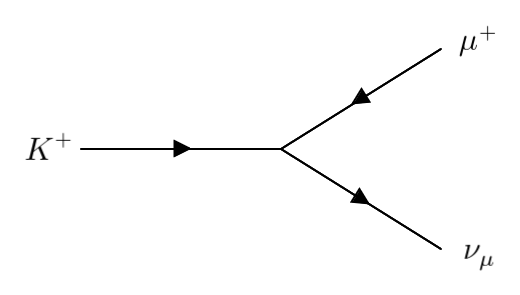
\includegraphics[width=\linewidth]{K_to_nu}
\caption{}
\label{fig:kaonnu}
\end{subfigure}
\hfill
\begin{subfigure}[h]{0.4\linewidth}
\centering    
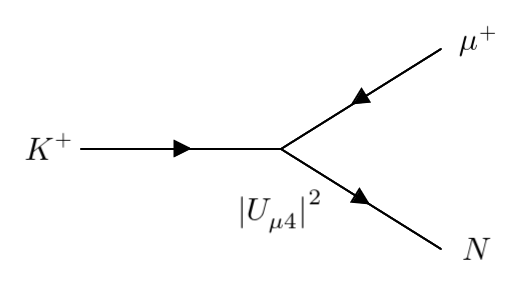
\includegraphics[width=\linewidth]{K_to_HNL}
\caption{}
\label{fig:kaonhnl}
\end{subfigure}%
%\hfill
\caption[Neutrino and Heavy Neutral Lepton Production Feynman Diagrams]
{
	Feynman diagrams of (a) $K^+ \rightarrow \mu^+ \nu_{\mu}$ and (b) $K^+ \rightarrow \mu^+ N$.% \cite{DavidePhD}.
}
\end{figure}

In general, the branching ratio $Br(m^+\rightarrow l^{+}_{\alpha}N)$ of a two-body decay of a charged meson $m^+$ into a lepton $l^{+}_{\alpha}$ ($\alpha=e,\mu,\tau$) and an HNL $N$ can be expressed in terms of the analogous branching ratio into an SM neutrino as follows \cite{HNLKelly}
\begin{equation}
	\label{eq:kaon_decay_hnl}
	Br(m^+\rightarrow l^{+}_{\alpha}N) = Br(m^+\rightarrow l^{+}_{\alpha}\nu_{\alpha})\left(\frac{|U_{\alpha 4}|^{2}}{1 - |U_{\alpha 4}|^{2}}\right)\rho_{N}\left(\frac{m^{2}_{l_{\alpha}}}{m^{2}_{m^+}}, \frac{m^{2}_{N}}{m^{2}_{m^+}} \right) 
\end{equation}
where $Br(m^+\rightarrow l^{+}_{\alpha}\nu_{\alpha})$ is the branching ratio of the charged lepton $m^+$ decaying into a lepton $l^+_{\alpha}$ and an SM neutrino $\nu_{\alpha}$, $m_{m^+}$ is the mass of the charged meson, $m_{l_{\alpha}}$ is the mass of the daughter lepton and $m_{N}$ is the mass of the daughter HNL.
The kinematic factor $\rho_{N}$ accounts for the available phase space of the daughter HNL in the decay and has the complete expansion as follows \cite{HNLKelly}

\begin{equation}
	\rho_{N}(x,y) = \frac{(x+y-(x-y)^{2})\sqrt{1+x^{2}+y^{2}-2(x+y+xy)}}{x(1-x)^{2}}
\label{eq:KinematicsFactor}
\end{equation}
where $x = m^{2}_{l_{\alpha}}/m^{2}_{m^+}$ and $y=m^{2}_{N}/m^{2}_{m^+}$.

Fig. \ref{fig:KinematicsFactor} depicts the kinematic factor $\rho_N$ of the HNL production compared to the analogous SM neutrino production as a function of the HNL mass.
Four HNL production channels that are probable at the BNB are shown: (1) $K^+ \rightarrow Ne^+$ in the dashed red line, (2) $K^+ \rightarrow N\mu^+$ in the solid pink line, (3) $\pi^+ \rightarrow Ne^
+$ in the dashed dark blue line and (4) $\pi^+ \rightarrow N\mu^+$ in the solid light blue line.  
Production channels associated with the $\tau$-flavour mixing are not shown since they are kinematically forbidden at the BNB.
The kinematic factor for each illustrated channel is constrained by the available mass after the two-body decay of the parent meson.
The upper limit of the HNL mass is therefore $m_{N} = m_{m^+} - m_{l_{\alpha}}$ ($\alpha=e,\mu$), as shown by the vertical grey lines.
Here it can be seen that the HNL production from $\pi^+$ decays limits the HNL mass to $< 140$ MeV while the HNL production from $K^+$ decays allows for the HNL mass up to 495 MeV. 
Thus, the search for HNLs presented here focuses on the HNL production channel from $K^+$ to probe mass as high as 495 MeV.

%Given the smaller masses of both a charged pion ($m_{\pi} = 140 $ MeV) and a charged kaon ($m_{K} = 494 $ MeV) compared to a tau ($m_{\tau}=1777 $ MeV), taus cannot be produced from meson decays in the BNB.
%Consequently, only electrons and muons are produced, limiting the flavours in the mixing $|U_{\alpha4}|^{2}$ to $\alpha = e, \mu$.

%Helicity Unsuppression i.e. K ->Ne and K->Nmu

%Enahancement factor??
Furthermore, the magnitude of the kinematic factor of the HNL production shown in Fig. \ref{fig:KinematicsFactor} is larger than 1 as compared to the analogous SM production.
This is because of the helicity suppression observed in mesons decaying into an SM neutrino having an opposite effect for mesons decaying into an HNL \cite{HNLKelly}.
Instead, it is helicity \textit{enhancement} due to HNLs being massive.
For the HNL production channel interested in this work, a significant enhancement is evident for the production rate of $K^+\rightarrow e^+ N$ being increased by a factor of $10^{5}$.
On the other hand, the kinematic factor of $K^+ \rightarrow \mu^+ N$ unfortunately only peaks at 4, implying a negligible enhancement in the production rate.

%The kinematic factor $\rho_{N}$ from Eq. \ref{eq:KinematicsFactor}, which also accounts for this enhancement, is plotted against the mass of HNLs in Fig. \ref{fig:KinematicsFactor}.

\begin{figure}[t] 
\centering    
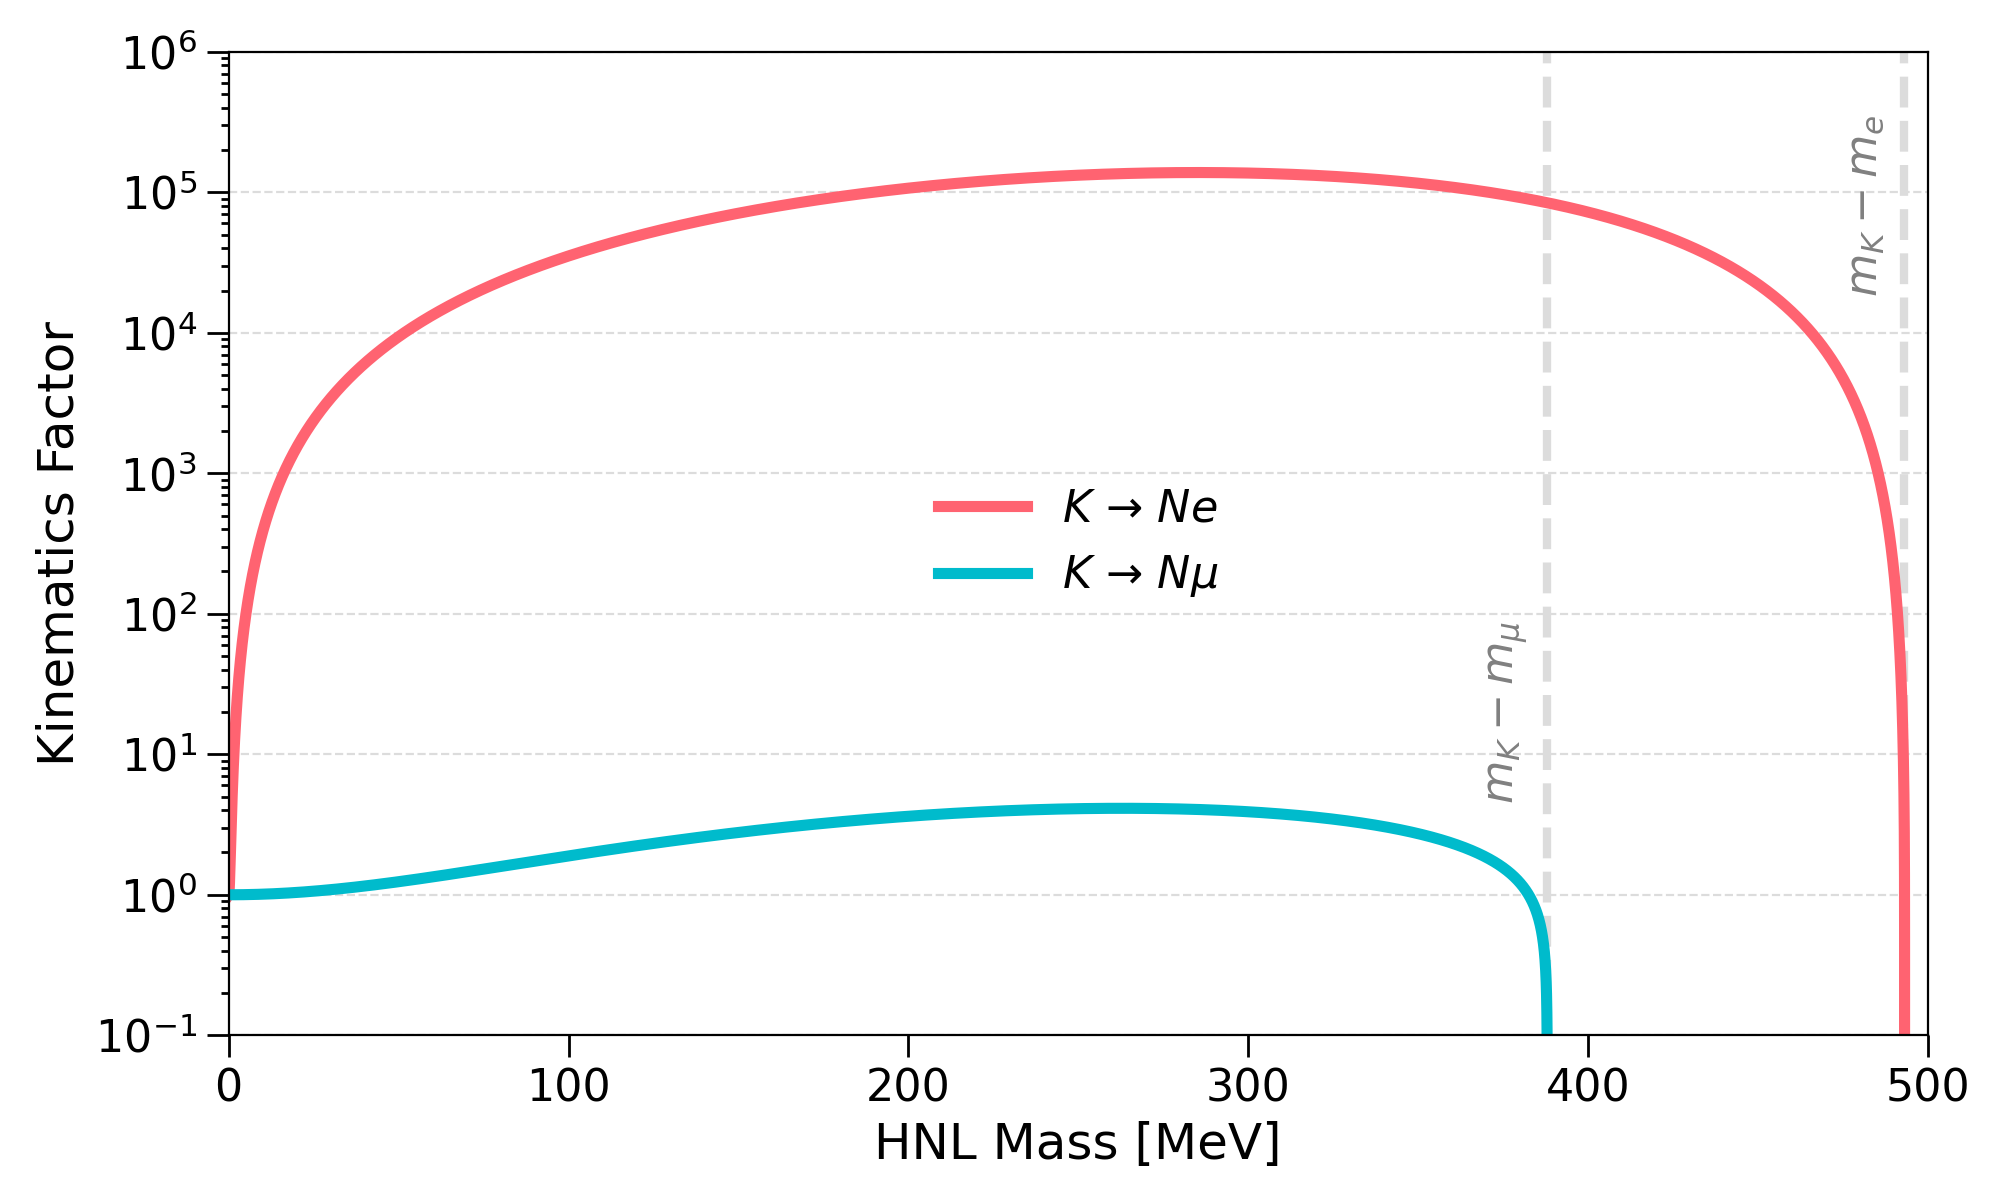
\includegraphics[width=1.0\textwidth]{kinematics_factor}
\caption[Kinematic Factor of Heavy Neutral Leptons]{
Plot showing the kinematic factor of the HNL production from meson decays as compared to the analogous SM neutrino production.
}
\label{fig:KinematicsFactor}
\end{figure}

\section{Decay Channels of Heavy Neutral Leptons}
\label{sec2Decay}

%HNLs are unstable particles and therefore decay in flight with a lifetime proportional to the mixing $|U_{\alpha4}|^{2}$ $(\alpha=e,\mu,\tau)$, 
%Since $|U_{\alpha4}|^{2}$ is the same coupling responsible for the HNL production, the observed event rate at the detector scales with $|U_{\alpha4}|^{4}$.

%DIF with coupling
For HNLs to be detected, they are hypothesised to be able to decay into SM observables \cite{HNLKelly}.
The proposed lifetime of HNLs should be sufficient so that an HNL produced from the BNB must survive long enough to reach the detector and then decay in flight.
At the mass range $< 495$ MeV, the kinematically-allowed decay channels of an HNL are as follows \cite{SBNHNL}

%Possible decay channel
\begin{equation}
\begin{split}
\label{eq:decay_channel}
	N\rightarrow e^{-}\pi^{+},\qquad 
	N\rightarrow \mu^{-}\pi^{+},\qquad
	N\rightarrow \nu \pi^{0},\qquad 
	N\rightarrow \nu \gamma,\qquad \\ 
	N\rightarrow \nu e^{-} e^{+},\qquad 
	N\rightarrow \nu \mu^{-} \mu^{+},\qquad 
	N\rightarrow \nu \mu^{-}e^{+},\qquad
	N\rightarrow \nu \nu \nu.   
\end{split}
\end{equation}
These decay channels here conserve the lepton number under the assumption that HNLs are Dirac particles with $L=+1$.
If HNLs are Majorana particles, such that the lepton number conservation is violated, then the charge conjugates for these decays that would be forbidden in the Dirac case are now allowed.

%Overall description of each BR channel

Fig. \ref{fig:branchingRatio} depicts branching ratios of decay channels shown in Eq. \ref{eq:decay_channel}, as a function of the HNL mass.
Solid lines are branching ratios via the $\mu$-flavour mixing ($[U_{e4}:U_{\mu4}:U_{\tau4}]=[0:1:0]$) and dashed lines are branching ratios via the $e$-flavour mixing ($[U_{e4}:U_{\mu4}:U_{\tau4}]=[1:0:0]$).
The branching ratios were plotted referencing decay widths from Ref. \cite {HNLBin, SBNHNL, HNLZarko}.
Decay widths of HNLs have been derived independently across various literature sources and an overview of discrepancies is summarised in Ref. \cite{HNLZarko}. 
The sources used here have been found to be in good agreement with each other.

For $m_{N} < 135$ MeV, the dominant branching ratio occurs in the channel $N\rightarrow \nu\nu\nu$ as shown by the light green lines.
However, this channel is almost unobservable since the detection of SM neutrinos relies on the already-small cross section of neutrino scattering with the detector material.
The other two channels in this mass range are $N\rightarrow \nu e^{-}e^{+}$ and $N\rightarrow \nu \gamma$, as shown by the light pink and grey lines.
The channel $N\rightarrow \nu \gamma$ is highly suppressed compared to the channel $N\rightarrow \nu e^{-}e^{+}$, and thus, the final state of $e^-e^+$ pair provides the best sensitivity within this mass range.

For $m_{N} > 135$ MeV, an HNL has sufficient mass to decay into either a neutral pion ($m_{\pi^{0}}=135$ MeV) or a charged pion ($m_{\pi^{+}}=140$ MeV). 
For the $e$-flavour mixing, the channel $N\rightarrow e^{-}\pi^{+}$ dominates over the channel $N\rightarrow \nu \pi^{0}$ across the mass range from 135 to 495 MeV, as shown by the dashed dark blue and dashed pink line respectively.
In the case of the $\mu$-flavour mixing, the leading channel within the mass range of $135 < m_{N} < 245 $ MeV is $N\rightarrow \nu \pi^{0}$ as shown by the solid pink line.
Beyond $m_{N} > 245$ MeV, equivalent to the mass of a muon and a charged pion, the dominant decay channel begins to shift to the channel $N\rightarrow \mu^{-}\pi^{+}$ as shown by the solid blue light. 
Finally, both channels $N\rightarrow \nu \mu^{-}e^{+}$ and $N\rightarrow \nu \mu^{-}\mu^{+}$ are not competitive compared to any other channels at the same mass value.  

\begin{figure}[ht!] 
\centering    
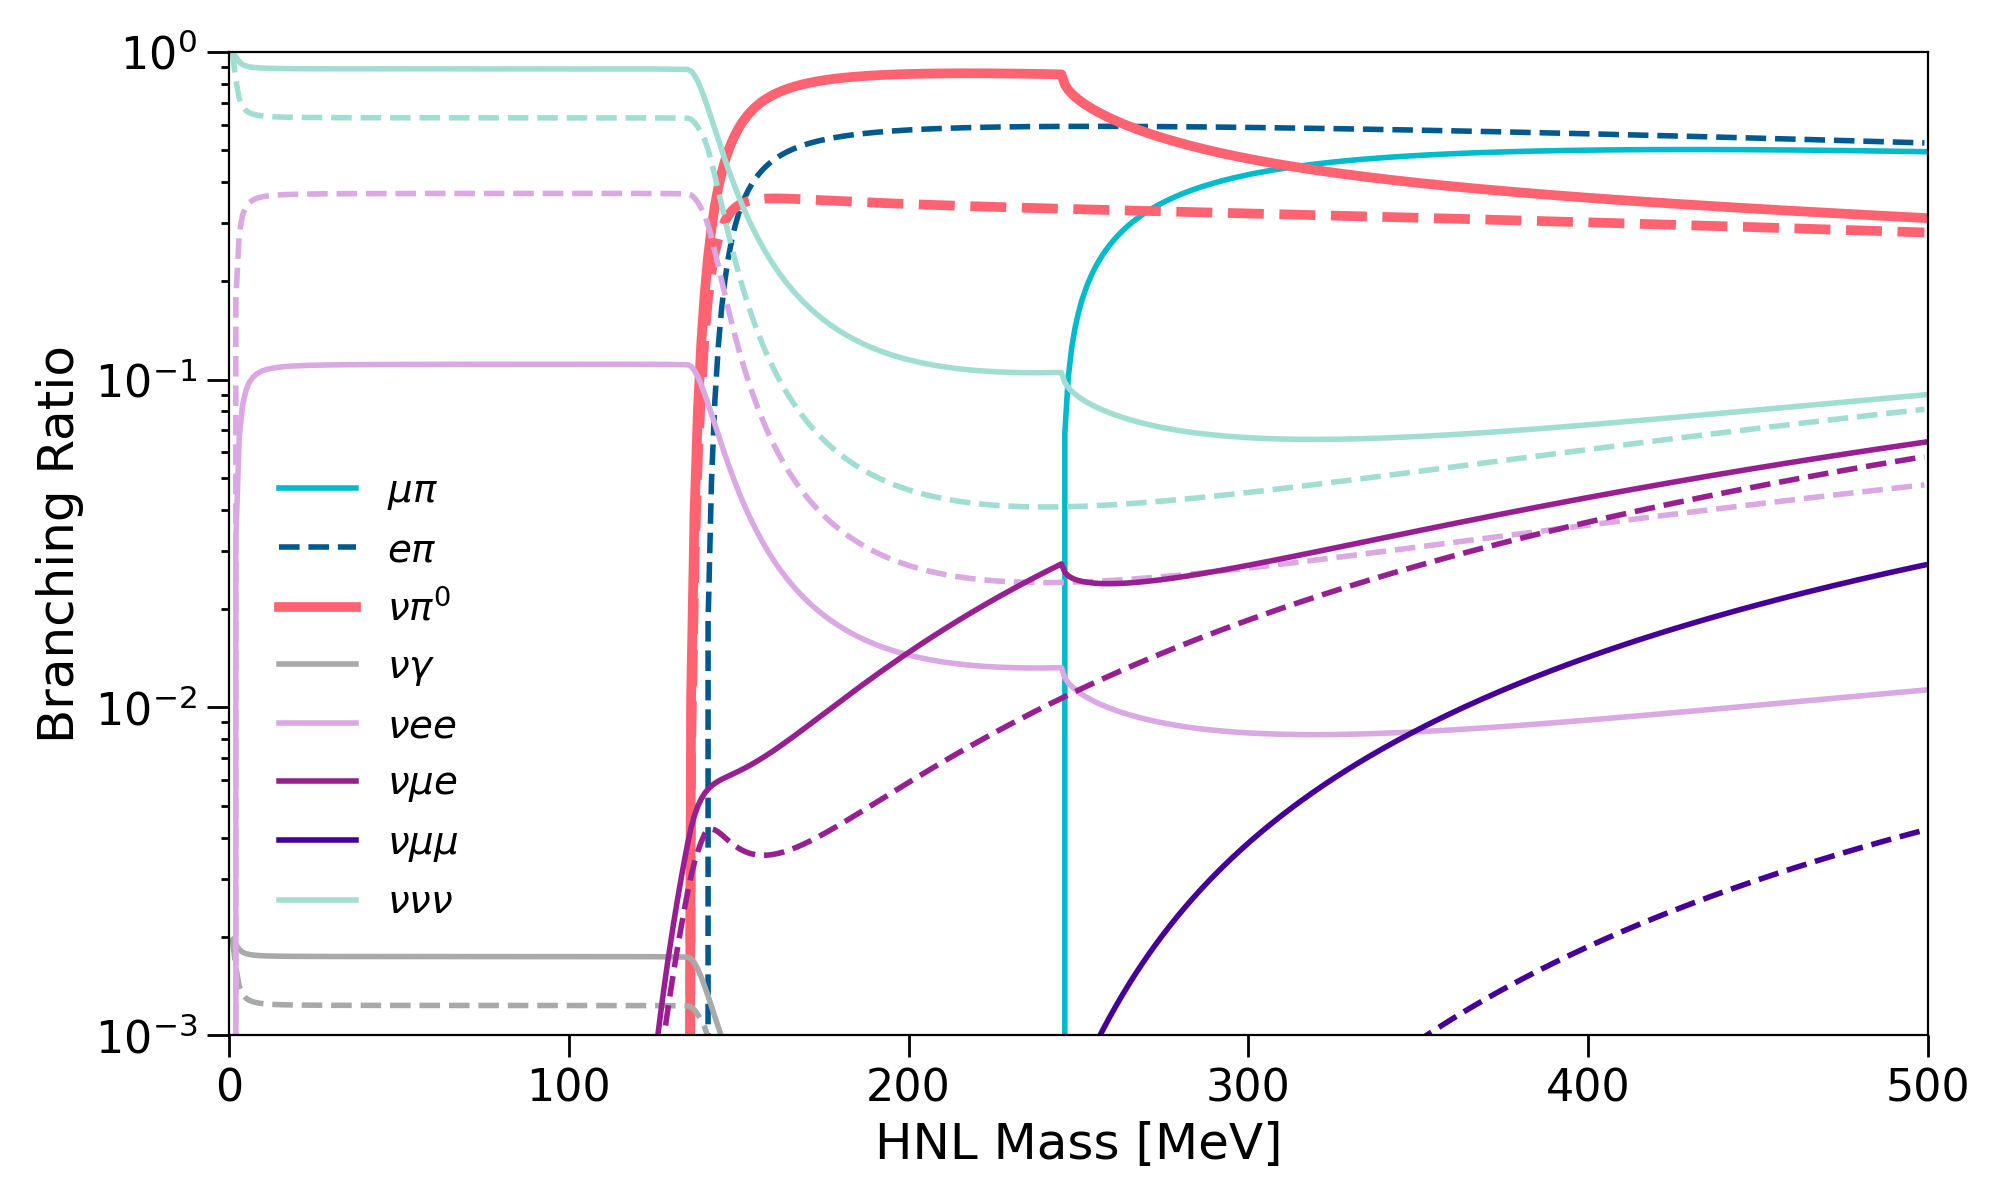
\includegraphics[width=1.0\textwidth]{branching_ratio}
\caption[Branching Ratio of Heavy Neutral Leptons]
{
Plot showing the branching ratio of probable decay channels of an HNL produced from the BNB.
}
\label{fig:branchingRatio}
\end{figure}

%This prompts a search focus on non-zero $|U_{\mu4}|^{2}$, assuming $|U_{e4}|^{2} = |U_{\tau4}|^{2} = 0$.  
%In this mass range, the primary mode of HNL production comes from  the decay of charged kaon, due to the kinematic constrains (See Sec. \ref{sec2Production}). 

Based on the assessment above it was decided in this work to focus on searching for HNLs through the decay channel $N\rightarrow\nu \pi^{0}$, which will be covered in Chapter \ref{ChapterSelect} and \ref{ChapterResult}.  
This is the leading channel of the $\mu$-flavour mixing within the mass range of $ 135 < m_{N} < 245 $ MeV.
Sensitivity in the same mass range of the $e$-flavour mixing has been extensively explored by many experiments as summarised by Ref. \cite{HNLWhitePaper}.
The decay width for the $N\rightarrow\nu \pi^{0}$ channel as taken from Ref. \cite{HNLZarko} is as follows
\begin{equation}
	\Gamma(N\rightarrow \nu \pi^{0}) = \frac{G_{F}^{2}m_{N}^{3}}{32\pi}f^{2}_{\pi}|U_{\mu4}|^{2}\left(1-\left(\frac{m_{\pi^{0}}}{m_{N}}\right)^{2}\right)^{2}
\label{eq:pi0}
\end{equation}
where $G_{F}$ is the Fermi constant, $f_{\pi}$ is the pion decay constant and $m_{\pi^{0}}$ is the mass of a neutral pion.
It is noted that the equivalent equations from Ref. \cite{SBNHNL, HNLBin} contain an additional factor of 2 in the denominator.
Eq. \ref{eq:pi0} was chosen from Ref. \cite{HNLZarko} since the source is more recently dated. 

%Decay signature in TPC
Fig. \ref{fig:HNLdecaydiagram} shows the diagram of the HNL decaying into the final state $\nu\pi^0$.
The SM neutrino is expected to leave no detectable signatures due to their very small scattering cross sections.
Meanwhile, the neutral pion is a particle made up of the superposition of the quark pair $u\overline{u}$ and $d\overline{d}$. 
The annihilation of quark and antiquark makes it a very short-lived particle with a mean lifetime of $8.52\pm0.18 \times 10^{-17}$ s \cite{PDG}.
The neutral pion decay has been measured to decay into two photons $98.823 \pm 0.034 \%$ of the time. 
Fig. \ref{fig:pi0decaydiagram} shows the Feynman diagram for the described decay.
The photon pair results in a clear signature inside a Liquid Argon Time Projection Chamber (LArTPC): two electromagnetic showers without any associated hadronic activities at the decay vertex.
This signal topology will face very challenging background separation from some SM neutrino channels also containing a $\pi^0$ in the final state.
As described in more detail in Chapter \ref{ChapterSelect}, differences in the final state kinematics from the HNL signal to the SM neutrino background enable an effective separation.

%this interaction constitutes the main background in
%Neutral current neutrino interactions that result in a neutral pion also share the same final state particles and thus, constituting the main background for this search.

%Nonetheless, . 

\begin{figure}[htbp!]
%\hfill
\begin{subfigure}[h]{0.49\linewidth}
\centering    
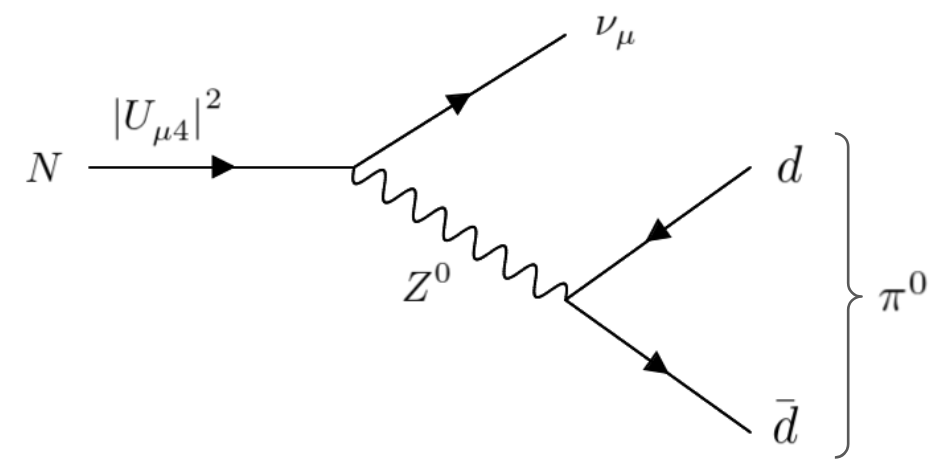
\includegraphics[width=\linewidth]{N_to_pi0_edit}
\caption{}
\label{fig:HNLdecaydiagram}
\end{subfigure}
\hfill
\begin{subfigure}[h]{0.49\linewidth}
\centering    
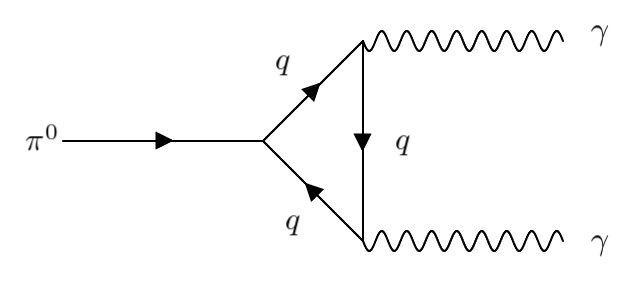
\includegraphics[width=\linewidth]{pi0_to_gam}
\caption{}
\label{fig:pi0decaydiagram}
\end{subfigure}%
%\hfill
\caption[Heavy Neutral Lepton and Neutral Pion Decay Feynman Diagrams]{
Feynman diagrams of (a) $N \rightarrow \nu \pi^0$ and (b) $\pi^0 \rightarrow \gamma\gamma$.
}
\end{figure}

%Dirac or Majorana Nature
%Dirac HNLs conserves the lepton number, while Majoranan HNLs violates the conservation and allows for forbidden decay channels    
%Majoranan HNLs violate the conservation of lepton numbers, whereas Dirac HNLs preserve it.
%Consequently, the expected event rate of Majoranan HNLs is double that of Dirac HNLs.

%Moreover, the polarisation of decay products differs between Majorana and Dirac HNLs for a neutral current process such as $\nu\pi^{0}$.

As previously discussed in Sec. \ref{sec2Production}, HNLs can be either Dirac or Majorana particles in nature.
The difference between Dirac and Majoranan HNLs is not only the lepton number conservation but also the polarisation of the decay products.
For the neutral current final state $\nu\pi^0$, Majoranan HNLs decay isotropically, whereas in the case of Dirac HNLs, the angular distribution of the daughter particles is no longer isotropic.
The helicity of the daughter neutrino determines the direction of the daughter neutral pion and the angular distributions of the two charge conjugate final states, $\nu\pi^{0}$ and $\overline{\nu}\pi^{0}$, add up to an isotropic distribution  \cite{HNLSilvia}.
As the neutrino is undetectable, the observed angular distribution of the neutral pion is expected to be insufficient to determine the Dirac or Majorana nature of HNLs.
For simplicity in this search for HNLs via the channel $\nu\pi^0$, it is therefore assumed that HNLs are Majorana particles.

\section{Previous Experimental Searches For Heavy Neutral Leptons}
\label{sec2Previous}

%Number of fermion families = Z boson decay for LH neutrinos, RH neutrinos is not constrained

%Overview of different types of searches
Searches for HNLs have been conducted by various experiments over the decades across a wide range of mass.
Oscillation experiments and precise $\beta$ decay experiments have probed HNLs in the mass range between eV and keV, neutrino beam dump experiments have targeted the MeV-scale HNLs and collider experiments have primarily explored HNLs with masses in the GeV-scale and above.
To date, no evidence of HNL existence has been found, and thus, experiments have set upper limits on the mixing $|U_{\alpha4}|^{2}$ $(\alpha=e,\mu,\tau)$.
Commonly, the contour on the experiment sensitivity is expressed in terms of the mixing $|U_{\alpha4}|^{2}$ as a function of the HNL mass.

Here, current experimental limits on HNLs around $\mathcal{O}$ (100 MeV) are presented, focusing specifically on the mass range of $ 0 < m_{N} < 265 $ MeV, which is relevant to the final states $\nu\pi^{0}$.
In this mass range, two key experimental methods are used, so-called peak searches and decay searches.
Peak searches probe only the production rate of HNLs, whereas decay searches probe both production and decay rates.
Fig. \ref{fig:sensitivity_theory} summarises the presented upper limits at 90\% confidence level (C.L.) from both experimental methods, with details on individual limit to be discussed in Sec. \ref{sec:peaksearch} and \ref{sec:decaysearch}.

\subsection{Peak Searches}
\label{sec:peaksearch}

Peak search experiments measure the energy spectrum  resulting from the decay of meson decay that would produce an HNL. 
Typically, the two-body leptonic decay of a meson is modelled as $m\rightarrow l + Missing$, where $m$ is the parent meson, a pion or a kaon, and $l$ is the daughter particle, a pion or a lepton \cite{OwenPhD}.
The \textit{missing} decay products are attributed to either HNLs or SM neutrinos.
HNLs are expected to exit the detector before decaying, whereas SM neutrinos escape the detector before interacting, serving as the primary background for this search.
Since the momenta of $m$ and $l$ are precisely measured, the missing invariant mass can therefore be derived as $m^{2}_{miss} = (P_{m} - P_{l})^{2}$, where $P_{m}$ and $P_{l}$ are the 4-momenta of the parent and daughter particle.
Given the near-zero mass of SM neutrinos, the mass of the daughter HNL can be treated as $m_{N} = m_{miss}$.
Consequently, an excess over the background at $m_{miss}$ potentially indicates the existence of HNLs.

To infer the upper limits on the mixing parameter, the flavour $\alpha$ ($\alpha =\mu,e$) of the daughter lepton determines the flavour of the mixing $|U_{\alpha4}|^2$, and the amplitude of the decay spectrum at $m_{miss}$ determines the upper limit.
Limits placed by the peak searches are insensitive to the Dirac or Majorana nature of HNLs as it does not impact the kinematics of the meson decay.
For the mixing $|U_{\mu4}|^{2}$, the most competitive limits have been established by the following experiments on the pion and kaon decay spectrum, and are plotted in Fig. \ref{fig:sensitivity_theory} as dashed lines.

\subsubsection{Pion Decay Spectrum Peak Searches}

\begin{coloritemize}
\item \textbf{SIN} (Swiss Institute for Nuclear Research) performed a peak search using stopped positive pions decay via the channel $\pi^{+} \rightarrow \mu^{+} + Missing$, with a scintillator in 1981 and a germanium detector in 1987.
The pion enabled probing HNLs within the low mass range of $\mathcal{O}$(10 MeV).
Upper limits of $|U_{\mu4}|^{2}$ were placed in the mass range 1--20 MeV at $10^{-4}$ \cite{SIN1, SIN2, SIN3}.

\item The \textbf{PIENU} collaboration at TRIUMF also searched for HNLs using stopped pions.
The most recent result in 2019 set the most stringent limits on $|U_{\mu4}|^{2}$ at $10^{-5}$ in the mass range of 15--34 MeV, extending beyond the result reported by SIN \cite{PIENU}.

\end{coloritemize}

\subsubsection{Kaon Decay Spectrum Peak Searches}

\begin{coloritemize}
\item The \textbf{KEK} collaboration conducted an experiment known as E89, which aimed to search for HNLs using the muon range spectrum resulting from stopped kaon decays during 1981--1982. 
Following this, experiment E104 in 1983 was carried out with an improved momentum resolution and background suppression.
The kaons were produced using a 0.5 GeV proton beam, and $3 \times 10^{6}$ muons from kaon decays were analysed using a magnetic spectrograph.
The E89 experiment result set limits on $|U_{\mu4}|^{2}$ between 10$^{-4}$--10$^{-6}$ within the mass range of 70--300 MeV.
Additionally, the combined results from the E89 and E104 experiments extended the sensitivity towards the lower mass range between 45--300 MeV, although these findings were unpublished at the time of writing and therefore plotted as the dotted line in Fig. \ref{fig:sensitivity_theory} \cite{KEK1, KEK2, KEK3}.

\item The \textbf{E949} collaboration at Brookhaven National Laboratory performed a kaon decay experiment using 21.5 GeV protons in 2002.
The analysis on the decays of $2 \times 10^{21}$ stopped kaons set limits on $|U_{\mu4}|^{2}$ at 10$^{-7}$--10$^{-9}$ within the mass range of 175--300 MeV \cite{E949}.

\item The \textbf{NA62} collaboration, a kaon decay experiment at the CERN super proton synchrotron, analysed $10^{8}$ stopped kaons from 400 GeV protons extracted from the synchrotron.
The first results from a data set in 2015 set upper limits on $|U_{\mu4}|^{2}$ at 10$^{-7}$--10$^{-6}$ for the HNL mass between 250--373 MeV.
Updated results using a larger dataset collected in 2016--2018 significantly improved the limits by an order of magnitude to 10$^{-8}$--10$^{-7}$, and extended the mass range to 200--384 MeV \cite{NA62A, NA62B}.
\end{coloritemize}

\subsection{Decay Searches}
\label{sec:decaysearch}

Decay searches look for decay products from HNLs.
HNLs are hypothesised to be produced outside of the detector and then decay in flight into SM observables inside the detector.
Different combinations of HNL production and decay channels yield different observed event rates of the decay products.
The flavour of the HNL production and decay channel both determine the flavour of the mixing $|U_{\alpha4}|^2$ and the observed event rate determines the upper limit on the mixing.  

Historically, decay searches have been performed in beam-dump experiments, which were designed explicitly to suppress SM background thereby enabling the search for rare decay processes.
Recently, modern neutrino oscillation experiments have emerged as competitive beam-dump experiments alongside their neutrino physics programme.
This is due to the resolution enhancement in their detection technologies that enable excellent SM background rejection, of which the Short-Baseline Near Detector is a prime example to be further detailed in this work. 
For the mixing $|U_{\mu4}|^{2}$ within the mass range of 0--265 MeV, the most competitive limits have been set by the following experiments using neutrino beams, and are plotted in Fig. \ref{fig:sensitivity_theory} as solid lines.

\begin{coloritemize}
%\item The \textbf{Super-Kamiokande} (SuperK) collaboration is the only decay search presented here that searched for HNLs from a non-beam source.
%Their dataset comprised of multi-GeV atmospheric neutrinos.
%In this case, HNLs were assumed to be produced from kaon and pion decays in atmospheric showers and consequently decay inside the SuperK detector.
%The result set a limit on $|U_{\mu4}|^{2}$ at $10^{-4}$--$10^{-7}$ within the HNL mass ranging from 70 to 386 MeV \cite{superk}.

\item The CERN \textbf{PS191} experiment in 1984 utilised an exposure of 19.2 GeV protons on a beryllium target, generating $10^{19}$ protons on target (POT).
The detector was positioned at 128 m from the target at an off-axis angle of $2.3^{\circ}$ to the beam.
The detector volume was filled with helium, which was a sparse medium to reduce background rates arising from SM neutrino interactions.
The large volume of 216 m$^3$ provided a high rate of HNL signals. 
Limits on $|U_{\mu4}|^{2}$ within the mass range of 120--350 MeV were placed at the level of 10$^{-5}$--10$^{-9}$ \cite{PS191A, PS191B}.
A re-evaluation in 2022 found the limits to be lower than the original published results \cite{PS191C}.
	
%\item The \textbf{T2K} collaboration recently searched for HNLs using the near detector ND280, located 280 m from the beam target at an off-axis angle of $2.04^{\circ}$.
%The analysis was performed on the data collected from 2010-2017, with a beam intensity of 30 GeV proton on graphite target and an exposure of $\approx 2 \times 10^{21}$ POT.
%The search was limited to the three argon gas TPC volumes, which minimised the neutrino background rate due to the low gas density.
%The results constrained the limits of $|U_{\mu4}|^{2}$ in the range of 10$^{-8}$--10$^{-9}$ for the HNL mass between 250--380 MeV \cite{T2KHNL}.
%The T2K collaboration has also presented results on $|U_{\mu4}|$ in the case where $|U_{e4}|$ and $|U_{\tau4}|$ are assumed to be non-zero and marginalised using results from other channels.

\item The \textbf{NuTeV} collaboration at Fermilab conducted HNL searches in 1996 using a high energy neutrino beam produced by protons accelerated from the Tevatron ring.
The dataset comprised an exposure of $3 \times 10^{18}$ POT with an energy of 800 GeV.
HNLs were produced from the $D$ mesons resulting from proton collisions with the target.
This enabled an exploration of the HNL mass up to 2000 MeV, surpassing any other beam-dump experiments described here.
The experiment established limits on $|U_{\mu4}|^{2}$ at the level of 10$^{-6}$--10$^{-7}$ within the mass range of 225--2000 MeV \cite{NuTeV}.

\item The \textbf{T2K} collaboration searched for HNLs using their near detector ND280 located off-axis to the beam target at an angle of $2.04^\circ$.
Only events occurring in the three gaseous TPC volumes were selected to minimise background from SM neutrinos.
A kinematic selection was performed on a dataset of $2\times10^{21}$ POT and no signals were observed.
The result constrained the mixing $|U_{\mu4}|^2$ at the level of $10^{-8}$--$10^{-9}$ in the mass range of $250$--$380$ MeV. 
The limit plotted in Fig. \ref{fig:sensitivity_theory} is a single-channel limit of $K^\pm \rightarrow N\mu^\pm$ and $N \rightarrow \mu^\pm\pi^\pm$.
A more stringent limit on $|U_{\mu4}|^2$ was also presented assuming the mixing $|U_{e4}|^2$ and $|U_{\tau4}|^2$ are non-zero.
This allows for a marginalised limit on $|U_{\mu4}|^2$ derived from other mixing results, which is not directly comparable here \cite{t2k}.

\begin{figure}[t!] 
\centering    
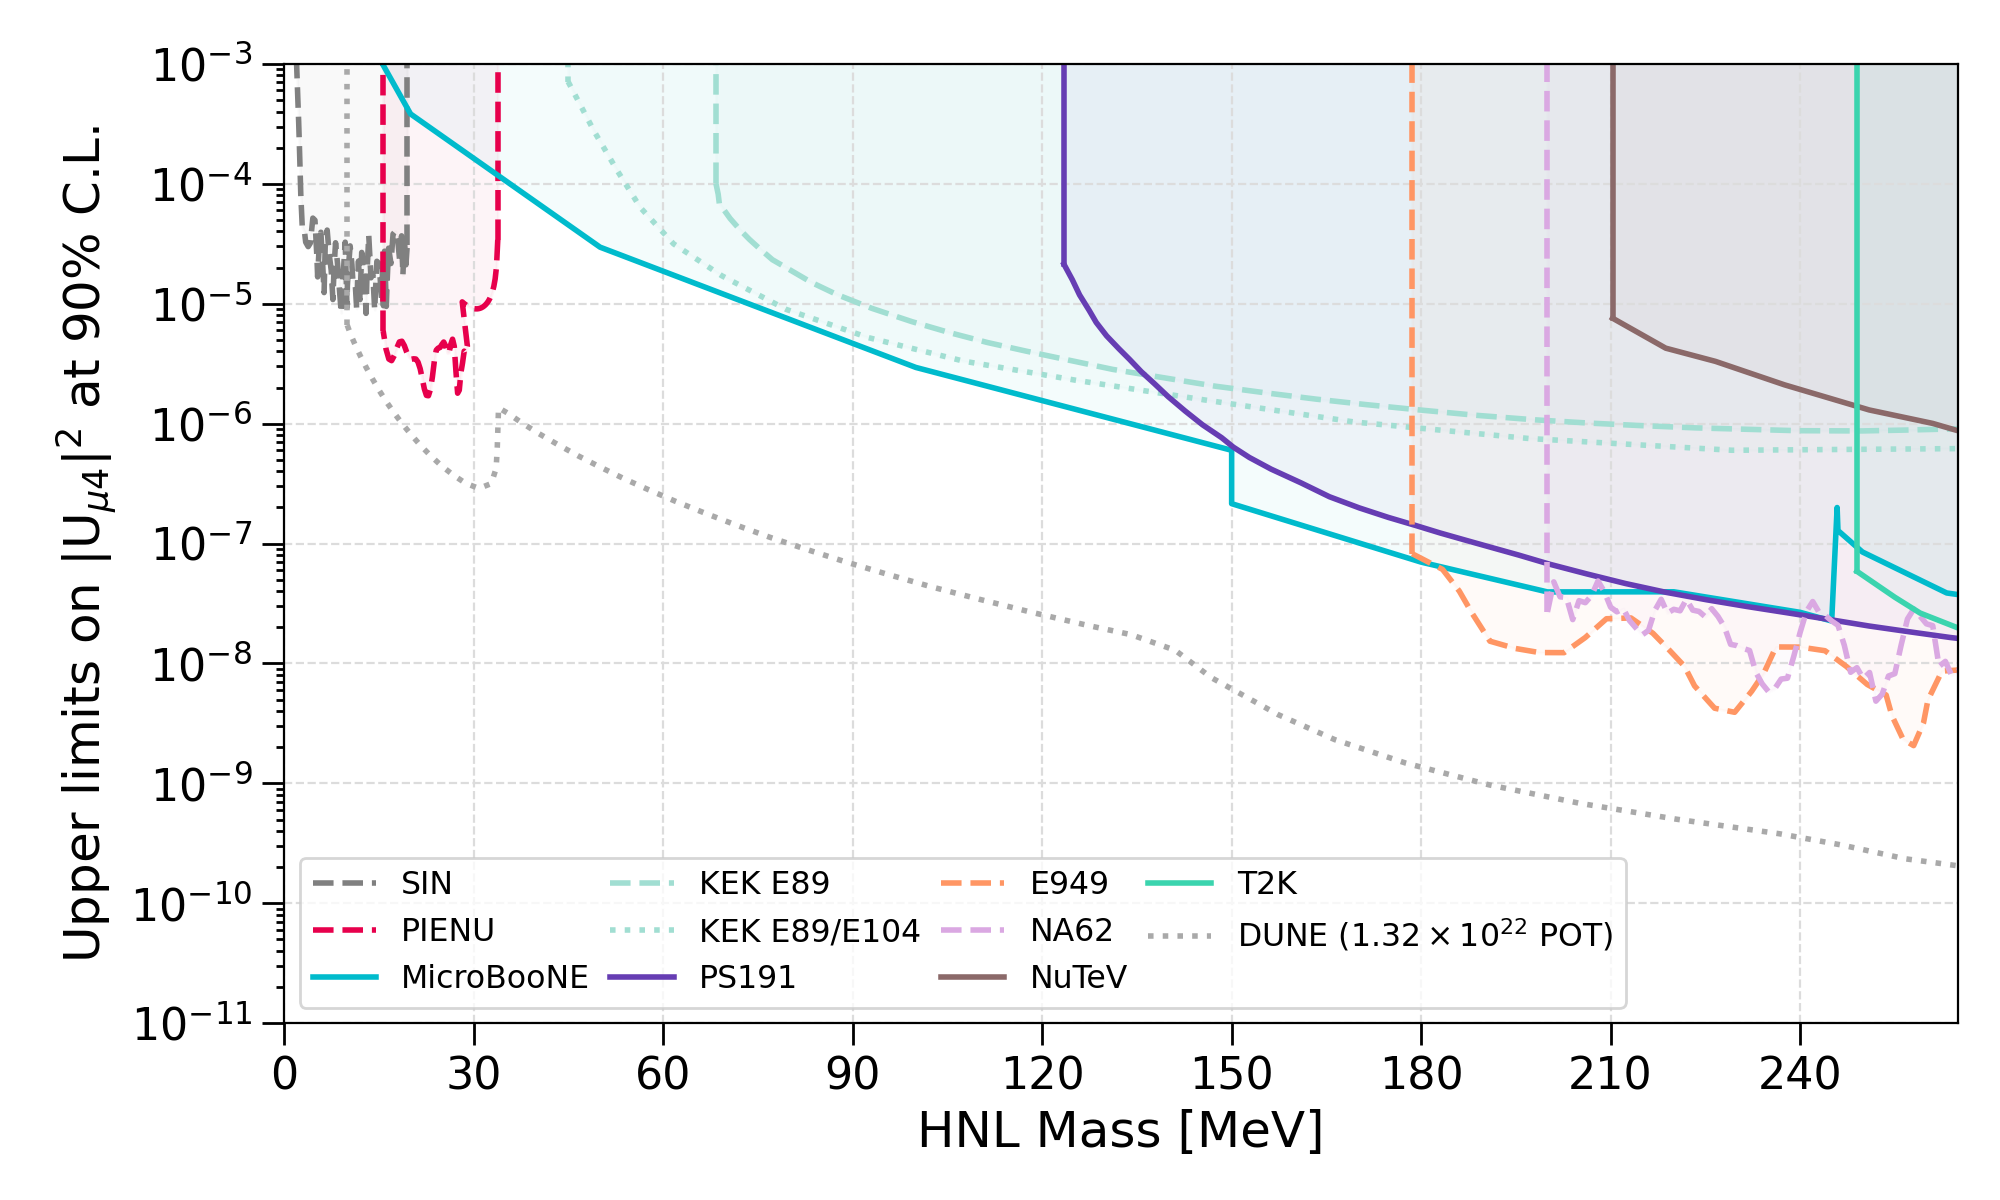
\includegraphics[width=1.0\textwidth]{sensitivity}
\caption[Experimental Upper Limits on The Mixing $|U_{\mu4}|^{2}$ of Heavy Neutral Leptons]{
Plot showing the upper limits on the mixing $|U_{\mu4}|^{2}$ at 90\% C.L. for Majoranan HNLs in the mass range of $0 < m_{N} < 265$ MeV.
}
\label{fig:sensitivity_theory}
\end{figure}

\item The \textbf{MicroBooNE} collaboration conducted a series of searches for HNLs using their LArTPC, with the first result in 2020 and subsequent results in 2022 and 2023.
The initial analysis was performed using an exposure of $2 \times 10^{20}$ POT obtained from the on-axis BNB.
A special delayed trigger was implemented to identify HNLs arriving at the detector later than SM neutrinos.
Limits on $|U_{\mu4}|^{2}$ were set at $10^{-7}$ for HNL masses spanning between 260--385 MeV.
The latter two searches focused on HNLs arising from kaons decays in the NuMI beam absorber, which arrived at the detector at an angle to SM neutrinos from the BNB.
The dataset included two runs with an exposure of $2 \times 10^{20}$ and $5.01 \times 10^{20}$ POT.
The combined results incorporated multiple HNL decay channels, probing a wide mass spectrum between 10--385 MeV.
Notably, these recent results set the most stringent limits to date on $|U_{\mu4}|^{2}$ at 10$^{-4}$--10$^{-7}$ within the mass range of 34--175 MeV, extending the findings from 2019 \cite{uboone1, uboone2, uboone3}.

\end{coloritemize}

\section{Concluding Remarks}
\label{sec2conclude}

HNLs are beyond SM particles that can provide a natural explanation not just for the mass generation of active neutrinos but also for their extreme lightness.
SBND, located only 110 m from the BNB, is capable of detecting HNLs resulting from meson decays in the beam, which then decay in flight inside the detector.
Fig. \ref{fig:sensitivity_theory} provides a summary of existing limits on the mixing $|U_{\mu4}|^2$ of HNLs in the mass range of 0--265 MeV, showing that this phase space has been well-explored by various experiments very recently.
For SBND to be competitive in this region, a high background rejection rate without comprising signal efficiency must be achieved when performing the kinematic selection.
This can be obtained by exploiting kinematic observables of HNL decay products for background rejection, including their delay compared to SM neutrinos as well as their boosted kinematics due to HNLs being massive. 
Toward this goal, novel detection technology and reconstruction techniques of SBND have demonstrated an excellent resolution in timing, spatial and calorimetry. 
The following Chapter \ref{Chapter3} and \ref{ChapterDetector} will provide an overall description of the LArTPC technology, followed by details of the detection technology at SBND.

%!TEX root = ../thesis.tex
%*******************************************************************************
%****************************** Third Chapter **********************************
%*******************************************************************************
\chapter{Physics of Liquid Argon Time Projection Chamber}
\label{Chapter3}
% **************************** Define Graphics Path **************************
\ifpdf
    \graphicspath{{Chapter3/Figs/Raster/}{Chapter3/Figs/PDF/}{Chapter3/Figs/}}
\else
    \graphicspath{{Chapter3/Figs/Vector/}{Chapter3/Figs/}}
\fi

%********************************** %Opening  **************************************

The Liquid Argon Time Projection Chamber (LArTPC) stands as a high precision detector in neutrino physics.
The detector was first proposed in 1977 by Rubbia \cite{Rubbia}, bringing together the time projection chamber technology developed by Nygren \cite{Nygren1, Nygren2} and the liquid argon ionisation chamber developed by Willis and Radeka \cite{WillisRadeka}.
LArTPC provides an excellent spatial, calorimetry and timing resolution while enabling a high neutrino interaction rate.
This novel technology remains the primary choice for many neutrino experiments at Fermilab.

%overview
The following chapter will delve into principle operations of a LArTPC.
Sec. \ref{sec3:overview} provides an overview of the design of a LArTPC and the choice of liquid argon.
In Sec. \ref{sec3:creation}, a comprehensive discussion is presented on particle interactions with the liquid argon to produce ionisation electrons and scintillation photons, which are the observables of a LArTPC.
Following that, Sec. \ref{sec3:propagation} outlines the propagation of the resultant electrons and photons through the liquid argon medium.
Finally, Sec. \ref{sec3:detection} provides an insight into the detection mechanism of the ionisation electrons and scintillation photons using wire planes and novel optical detection technologies respectively.

\newpage

%********************************** %First Section  **************************************
\section{Overview of LArTPC}
\label{sec3:overview}
%1: Introduction
The Liquid Argon Time Projection Chamber (LArTPC) is the technology of choice for Fermilab's neutrino program, due to its ability to facilitate a high rate of neutrino interactions while maintaining an exceptional spatial, calorimetry, and timing resolution. 
Moreover, the abundant availability of argon is ideal for scaling detectors to a large target mass, reaching up to tens of kilotons of liquid argon.
Notably, the Short-Baseline Neutrino (SBN) programme \cite{SBNProgram} comprises of three LArTPC experiments of sizes in the hundreds of tons, located along the Booster Neutrino Beam (BNB): the Short-Baseline Near Detector (SBND) \cite{sbnd_det}, MicroBooNE \cite{ubooneDet}, and ICARUS \cite{icarus_det}.
This novel technology will also be utilised at the upcoming long baseline Deep Underground Neutrino Experiment (DUNE), of which its far detector is composed of four LArTPCs, boasting a total volume of 70 kilotons \cite{dunefd_det}.

%2: LArTPC description and figure 
A diagram illustrating the general operation principle of a LArTPC is provided in Fig. \ref{fig:LARTPC}.
Charged particles resulting from a neutrino interaction ionise argon atoms as they traverse through the detector medium, also producing scintillation photons in the process.
A high negative voltage is applied at the cathode plane, creating an electric field under which the ionisation electrons drift towards the anode.
\begin{figure}[htbp] 
\centering    
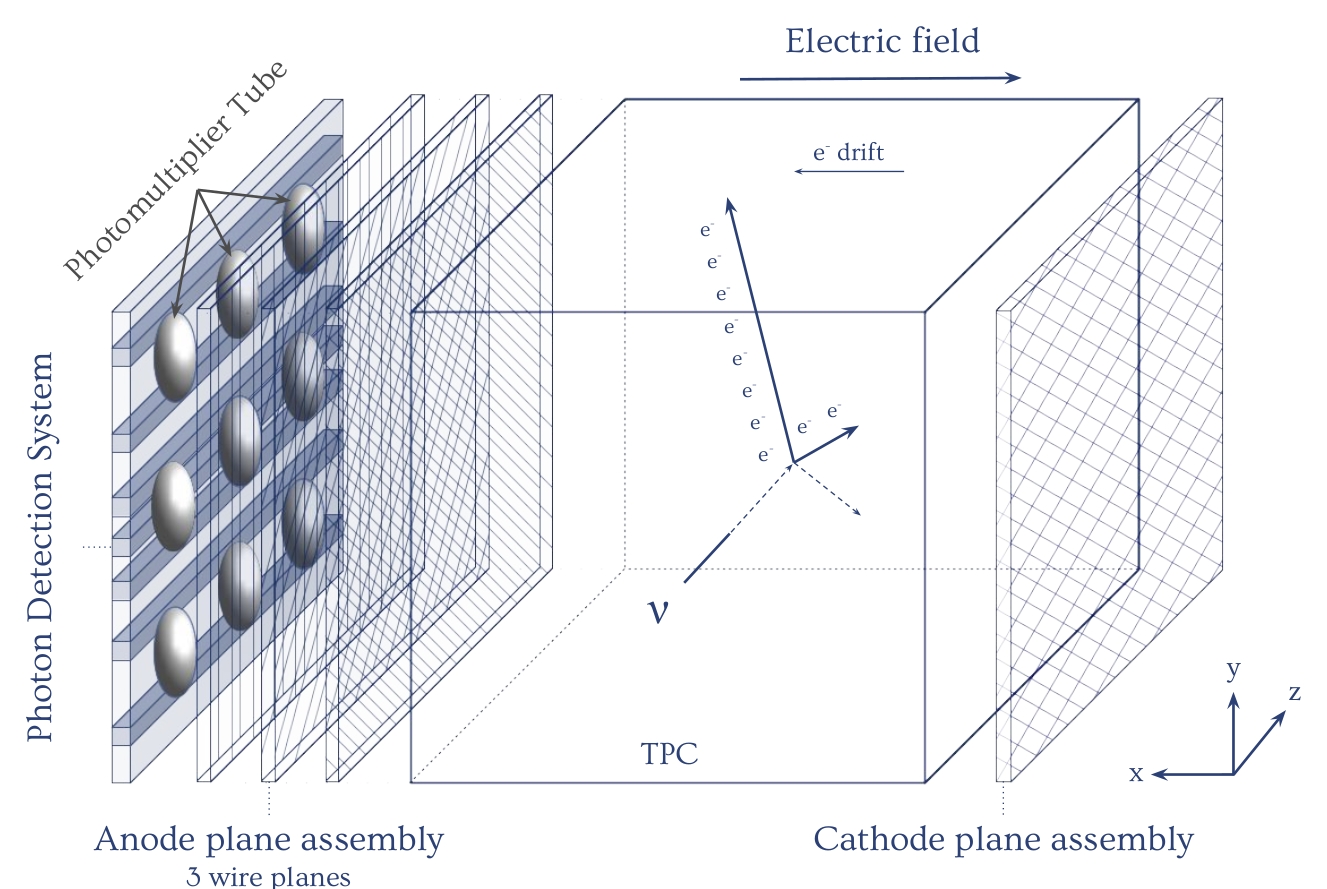
\includegraphics[width=0.65\textwidth]{LARTPC}
\caption[LARTPC]{
Illustration of a general LArTPC, depicting a cathode plane assembly on the edge of the TPC and an anode plane assembly in the opposite side along the x-direction.
Behind the wire planes at the anode is the PDS made up of 9 PMTs.   
An example neutrino interaction is shown, which produces two charged tracks (solid lines) and a neutral track (dashed line). 
The charged tracks produce ionisation electrons, which drift towards the anode in the opposite direction of the electric field. 
The neutral track does not ionise the argon atoms and thus is not directly visible in the detector. \cite{RhiannonPhD}.
}
\label{fig:LARTPC}
\end{figure}
Once arrive at the anode, the ionisation electrons induce signals on the inner wire planes and finally collected on the outermost plane.
The combination signals from these planes result in a high granularity three dimensional image of the interaction.
Since the wire planes are transparent to the scintillation photons, an additional Photon Detection System (PDS) is installed behind the wire planes, gaining additional calorimetry and precise timing information of the interaction.

%add why argon as target material
Specifically chosen for measuring neutrino cross sections, liquid argon has a high density of 1.39 gcm$^{-3}$ and a high atomic mass of 40.
The probability of neutrino interactions increases with the number of nucleons in the detector volume, and liquid argon, therefore, enables a high rate of neutrino interactions.
Furthermore, given that argon is a noble element, the energy deposited by particles traversing through the medium can only be used for ionising electrons and producing scintillation photons.
This maximises the efficiency of energy transfer into observable signals for detection.
Additionally, liquid argon has a very high electron mobility, allowing for ionisation electrons to quickly drift under an electric field.
Recent technology advancements in purifying argon has resulted in stable and ultra pure argon, which ensures that electrons can transverse the drift distance towards detection without being captured \cite{ubooneEtime}.
Consequently, liquid argon continues to stand out as an advantageous target material for neutrino experiments. 


\section{Particle Interactions in Liquid Argon}
\label{sec3:creation}

%Ionisation
\subsection{Ionisation Electrons}

%Energy loss profile
Charged particles traversing a medium, such as liquid argon, undergo energy loss via ionisation, producing electrons. 
The typical energy loss profile is illustrated in Fig. \ref{fig:BetheBloch}, specifically for a muon traversing in a copper medium; however, the underlying principle is applicable to liquid argon.
The plot depicts the stopping power, which is the energy loss per unit length divided by the density of the target medium, against the momentum of the traversing particle \cite{Passage}.
In the range of energy relevant in liquid argon, heavy particles such as muons, pions, and protons, experience energy loss as described by the Bethe-Bloch formalism.
On the other hand, for lighter and highly relativistic particles, such as > 100 MeV electrons in liquid argon, the primary mechanism for energy loss is through radiative effects.
An example depicting both of these event topologies is presented in Fig. \ref{fig:track_shower}.

\begin{figure}[htbp] 
\centering    
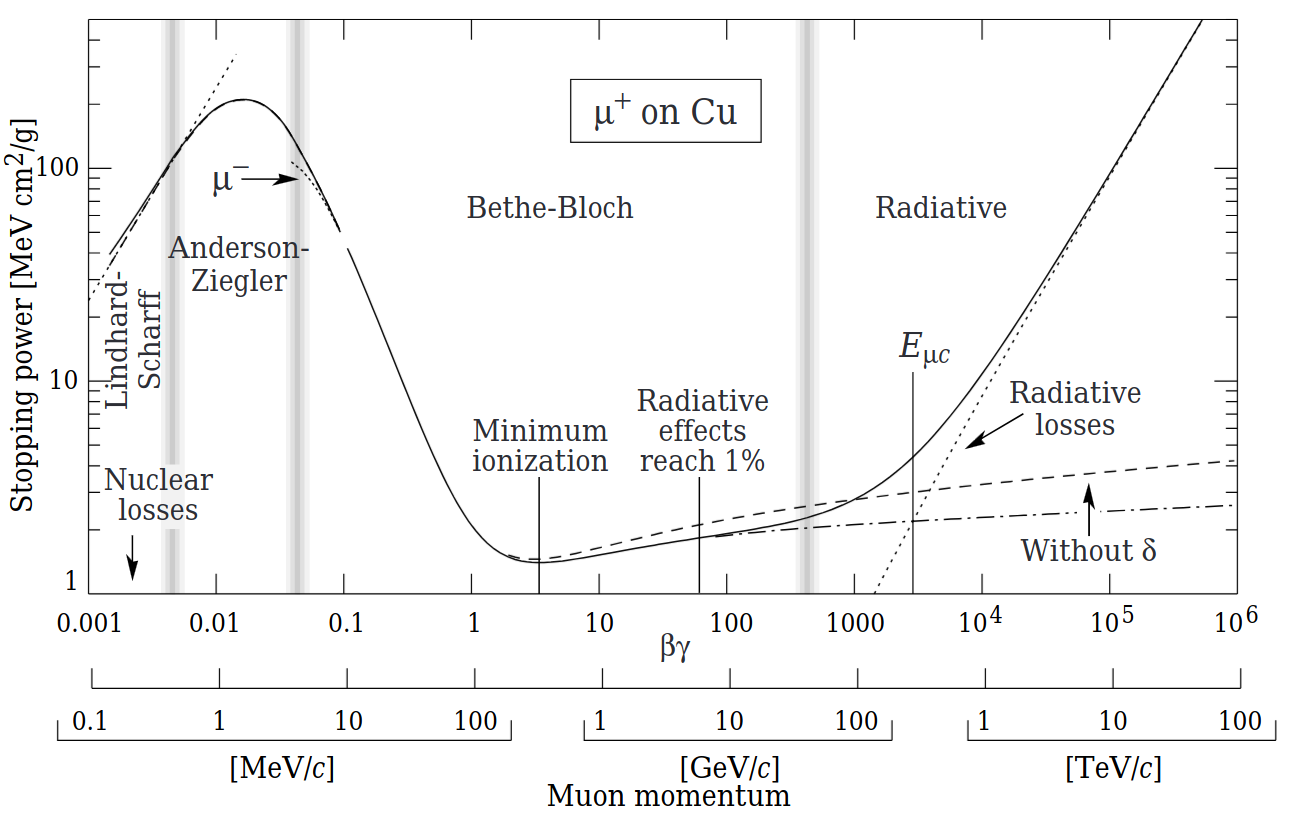
\includegraphics[width=0.85\textwidth]{BetheBloch}
\caption[BetheBloch]{
Example of particle energy loss in matter for a muon traversing a copper medium.
Energy loss for tracks is described by the Bethe-Bloch regime, followed by a rise in stopping power as the particle comes to a stop, representing the Bragg Peak.
Energy loss for showers is described by the radiative regime.
Fig. from \cite{Passage}.
}
\label{fig:BetheBloch}
%\end{figure}

%TODO: track and shower event display
\hfill
\break
%\begin{figure}[btp] 
\centering    
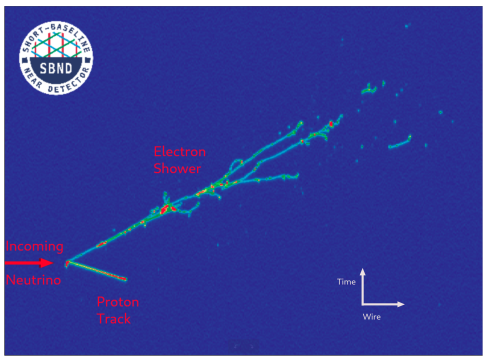
\includegraphics[width=0.6\textwidth]{temp}
\caption[track_shower]{
An event display of a charged current neutrino event, showing a track-like and a shower-like topology.
The track topology is from energy deposition of a proton, whereas the shower topology is from energy deposition of an electron interacting in liquid argon.
}
\label{fig:track_shower}
\end{figure}

%Track like
Muons, pions and protons interact electromagnetically with argon atoms as they propagate through liquid argon, primarily via Multiple Coulomb Scattering (MCS), freeing electrons along their trajectories.
These trajectories, typically following straightly lines, are referred to as \textit{tracks}.
As shown in Fig. \ref{fig:BetheBloch}, the MSC process is dependent on the momentum of the traversing particle.
Within the momentum range of 1 - 100 MeV, the energy deposited per unit length via ionisation, denoted as $dE/dx$, remains generally constant, often referred to as Minimum Ionising Particle (MIP).
In this MIP region, $dE/dx$ is described by a Landau-Gaussian Convolution. 
When the particle comes to a stop, the energy deposited arises, forming the so called Bragg peak.
The energy loss profile described here is dependent on the mass of the traversing particle, making it a valuable tool for Particle IDentification (PID) \cite{argoneut}.
This method is the most effective for protons separation from muons and pions, due to protons being significantly heavier.


%Shower like
Electrons with energy above the critical energy, which is the point at which losses due to ionisation are equal to losses from radiation, deposit energy via radiative effects \cite{uboone_gamma}.
The critical energy for electrons in liquid argon is 39 MeV.
This process typically results in cones of electromagnetic activities, commonly referred to as \textit{showers}. 
In the energy range relevant in a LArTPC, typically between 0.1 - 1 GeV, showers deposit energy over a distance of $\sim$1 m, and the shower length is logarithmic in energy.

Photons, being neutral particles, can travel some distance without ionising and before depositing energy inside the liquid argon \cite{uboone_gamma}.
This creates a gap between the interaction vertex and the start of the shower, known as the \textit{conversion gap}.
Photons can deposit energy via two interaction modes as illustrated in Fig. \ref{fig:uboone_gamma}.
At low energies, the primary process is Compton scattering, of which the radiation length is 14.1 cm.
However, at higher energies, pair production becomes the dominant effect, producing an $e^{+}e^{-}$ pair.
\begin{figure}[htp] 
\centering    
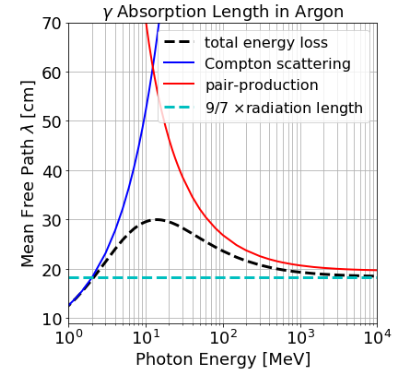
\includegraphics[width=0.40\textwidth]{uboone_gamma}
\caption[uboone_gamma]{
Plot showing the mean free path of photons traversing in liquid argon as a function of their energies.
In cyan is the conversion gap of 18.1 cm, which is 9/7 the radiation length.
Fig. from \cite{uboone_gamma}.
}
\label{fig:uboone_gamma}
\end{figure}
Both the energy loss profiles and the conversion gaps can be utilised to distinguish between electrons and photons. 


\subsection{Scintillation Photons}

%Scintillation light
Charged particles traversing liquid argon also produce scintillation photons, through two different processes, both resulting in an argon excimer ($Ar_{2}^{*}$) shown in Fig. \ref{fig:recomb_diagram}.
The first process is known as a self-trapped exciton.
This begins when the charged particle does not have sufficient energy for ionisation, and hence, it excites the argon atom upon collision instead.
The excited argon atom self-traps with another argon atom, forming an argon excimer .
The second process is known as recombination.
Ionisation in liquid argon produces a free electron and an argon ion ($Ar^{+}$).
The electron can either escape and drift towards the anode for detection, or recombine with an argon ion and an argon atom, forming an argon excimer.
The resulting argon excimer is short-lived and undergoes radiative decay into two ground-state argon atoms.
This process produces scintillation photons with a wavelength of 128 nm in the Vacuum UltraViolet (VUV) range \cite{Lariat}.

\begin{figure}[hbtp] 
\centering    
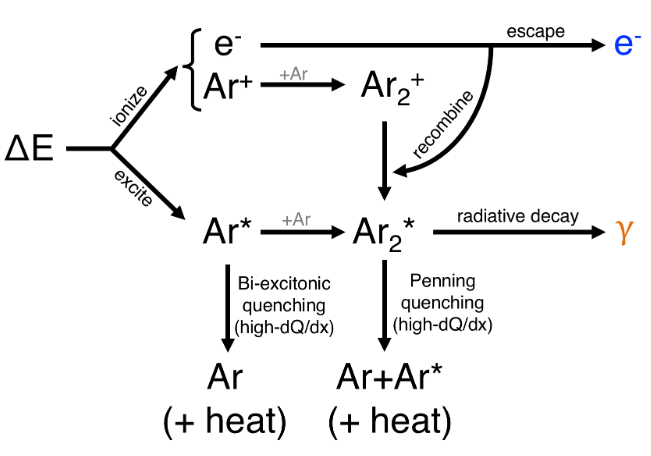
\includegraphics[width=0.6\textwidth]{recomb_diagram}
\caption[recomb_diagram]{
Diagram illustrating the production of ionisation electrons and scintillation photons from energy deposition processes in liquid argon.
Fig. from \cite{Lariat}.
}
\label{fig:recomb_diagram}
\end{figure}

The timing constant of the radiative decay depends on the excitation state.
The singlet state has a shorter mean lifetime with a decay constant $\tau_{1} \approx 6 - 7$ ns, while the triplet state has a longer mean lifetime with a decay constant $\tau_{3} \approx 1.5 - 1.6$ $\mu$s \cite{photon_lifetime}.
These are referred to as the fast (or prompt) and slow (or late) components, respectively. 
The time-dependent probability of light emission in pure liquid argon can therefore be modelled as
\begin{equation}
	l(t)=\frac{A_{1}}{\tau_{1}}\exp{\left(-\frac{t}{\tau_{1}}\right)} +\frac{A_{3}}{\tau_{3}}\exp{\left(-\frac{t}{\tau_{3}}\right)}
\end{equation}
where $A_{1}$ and $A_{3}$ are the decay amplitudes of the singlet and triplet state. 

%TODO: Add time distribution graph, see Patricks

%Quenching
Liquid argon serves as an excellent medium for producing scintillation photons, such that the light yield is as high as $\sim$40,000 photons per MeV of deposited energy in the absence of an electric field \cite{light_yield}.
In a typical electric field at 500 V/cm, as configured in SBND, the light yield decreases to $\sim$20,000 photons per MeV of deposited energy, due to free electrons being drifted before recombination can occur \cite{light_yield_Efield}.
Furthermore, high ionisation density may lead non-radiative quenching effects \cite{Lariat}.
Contaminants in liquid argon, such as oxygen and nitrogen, can absorb energy from argon excitons and excimers, without emitting any photons.
 
\subsection{Recombination}
\label{sec:recomb}
%Recombination

The electron-ion recombination, as depicted in Fig. \ref{fig:recomb_diagram}, occurs almost immediately within 1-2 ns following the ionisation process.
The electron recombination survival probability, also known as \textit{recombination factor} $R$, is defined as following 
\begin{equation}
	R=W_{ion} \cdot \frac{dE/dx}{dQ/dx}
\end{equation}
where $W_{ion} = 23.6$ eV is the energy required to ionise an argon \cite{ion_e} and $dQ/dx$ and $dE/dx$ is the charge and energy loss per unit length respectively. 
In Fig. \ref{fig:recomb_graph}, a comparison of various recombination models with a non-linear dependence on $dE/dx$ is presented.
The Birks model has been disfavoured due to spurious values at high charge density \cite{argoneut_recomb}.
The Box model is based on columnar theory around the charge deposition, and its modified version with experimentally-derived parameters measured by the Argoneut experiment, has improved agreement with data at low charge density.
The modification accounts for the presence of an electric field and local ionisation density.
\begin{figure}[thp] 
\centering    
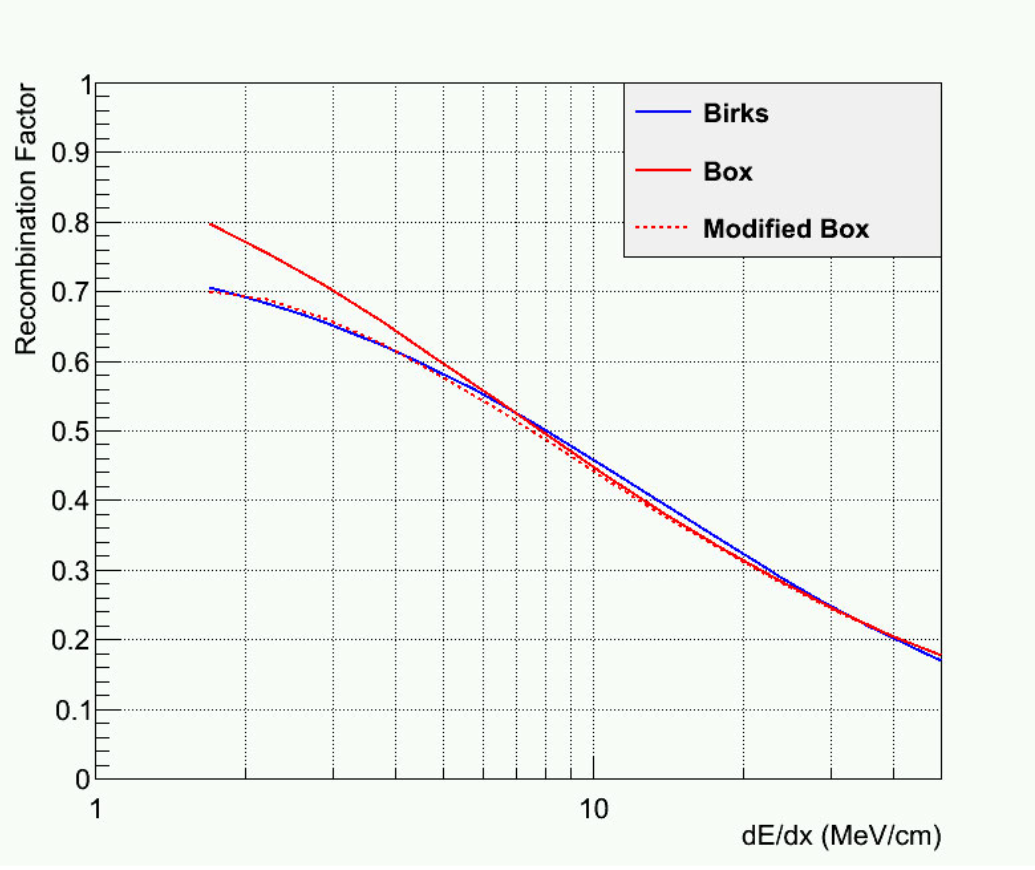
\includegraphics[width=0.6\textwidth]{recomb_graph}
\caption[recomb_graph]{
Graph showing recombination factor as a function of deposited energy density at an electric field of 500 V/cm. 
Fig. from \cite{argoneut_recomb}.
}
\label{fig:recomb_graph}
%\end{figure}
%\begin{figure}[tp] 
\hfill
\break
\break
\centering    
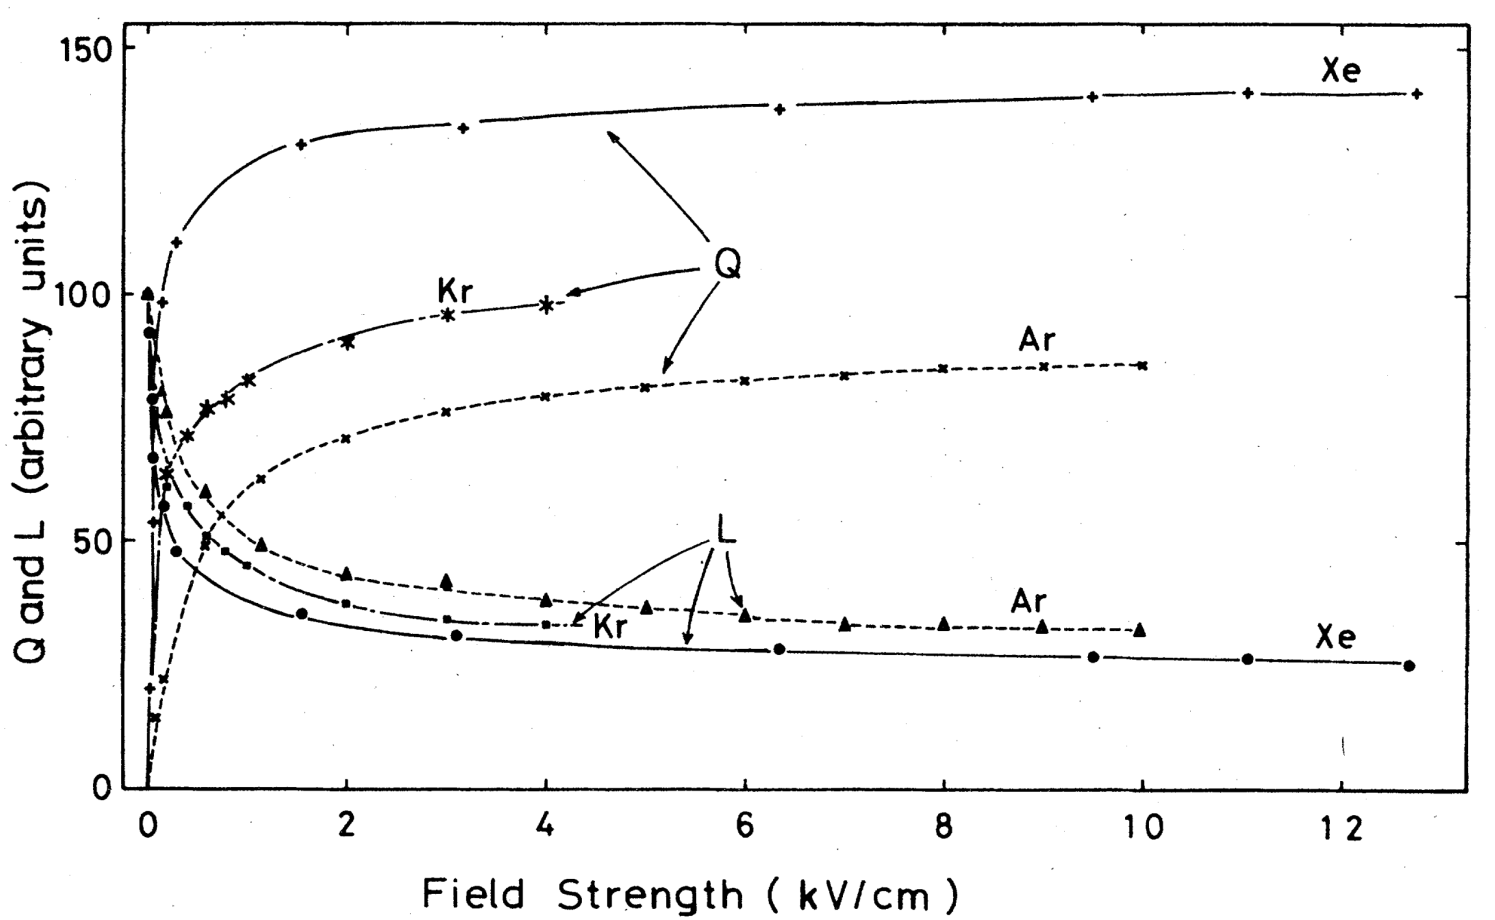
\includegraphics[width=0.7\textwidth]{QLAnti}
\caption[QLAnti]{
Charge ($Q$) and light ($L$) anti-correlation for noble elements like argon, xenon and krypton as a function of the electric field strength.
Fig. from \cite{QLAnti}.
}
\label{fig:QLAnti}
\end{figure}

%A popular model to describe this effect is the Box Model, based on columnar theory around the charge deposition \cite{box_model}. 
%The inverse Box Model equation is formulated as \cite{argoneut_recomb}
%\begin{equation}
%	\frac{dE}{dx} = \frac{1}{\beta}\left[ \exp{\left( \beta W_{ion}  \frac{dQ}{dx}\right)} -\alpha \right]
%\end{equation}
%where $\alpha$ and $\beta$ are experimentally derived parameters.
%Recombination is highly dependent on the electric field and the local charge density, which is folded into the $\beta$ parameter.
%ArgoNeuT experiment recently conducted a data-driven study on recombination in LArTPC, resulting in the ``Modified Box Model" with parameter $\alpha = 0.93$ and $\beta = 0.30 $ MeV/cm \cite{argoneut_recomb}.
%If not taken into account, the recombination can result in underestimating energy loss due to ionisation.

The dependence of recombination on the electric field leads to an anti-correlation between the charge and light yield $Q$ and $L$ respectively, such that \cite{argoneut_recomb}
\begin{gather}
	Q = N_{i}R \\ 
	L = N_{ex} + N_{i}(1 - R)
\end{gather}
where $N_{i}$ is the number of electron-ion pairs and $N_{ex}$ is the number of argon excitons.
A stronger electric field results in a higher number of ionization electrons being separated from the argon ions and drifted towards the anode for detection before recombination can occur. 
Conversely, scintillation photons are produced in the recombination process.
In the presence of an electric field, recombination decreases, leading to a reduction in light yield.
Furthermore, the recombination factor can be influenced at a local scale due to ionization density resulting from interacting particles.
Fig. \ref{fig:QLAnti} illustrates the anti-correlation between charge and light yield as a function of electric field strength for various noble elements.
The SBND detector operates with an electric field of 500 V/cm, a region where the energy deposition to ionization electrons and scintillation electrons are approximately equal \cite{QLAnti}.

%TODO: Check Gray's paper on recombination dependence of track angular
\section{Particle Propagation in Liquid Argon}
\label{sec3:propagation}

%Transportation of ionised electrons, diffusions, impurities
\subsection{Electrons Drift}
\label{sec:edrift}
\subsubsection{Diffusion}

%Electron drift under electric field
Ionised electrons that do not recombine drift towards the anodes under the effect of an electric field.
In a typical LArTPC with an electric field of 500 V/cm and a temperature of 87 K, the drift velocity of electrons is approximately 0.16 cm/$\mu$s \cite{drift_vel}.
As the electrons drift, they undergo diffusion, causing perturbations in their trajectories due to various effects, such as inelastic collisions.
Diffusion causes the shape of a cloud of electrons produced in a point like energy deposition to grow in volume while drifting.
The effects increase with respect to the drift distance, smearing both spatial and temporal resolutions.
The observed Gaussian profile $\sigma$ resulting from the response function of a charge deposition on the wire can therefore be modelled as \cite{uboone_diff} 
\begin{equation}
	\sigma^{2} (t) = \sigma^{2}_{0} + \left(\frac{2D}{v^{2}_{d}}\right)t
\end{equation}
where $\sigma_{0}$ is the initial profile without diffusion, $v_{d}$ is the drift velocity, $t$ is the drift time and $D$ is the diffusion coefficient.

Diffusion is parameterised in both the longitudinal direction $D_{L}$ and the transverse direction $D_{T}$, which are parallel and perpendicular to the drift direction respectively.
Longitudinal diffusion affects the temporal resolution, as individual electrons arrive at the wire either earlier and later relative to the electron cloud moving at the average drift velocity.
Transverse diffusion broadens the cross section of the electron cloud arriving at the original wire, causing electrons migrating to neighbouring wires.
Under the same conditions as the SBND detector, the diffusion coefficients have been measured to be $D_{L} = 7.2 $ cm$^{2}$/s and $D_T = 12.0 $ cm$^{2}$/s \cite{drift_vel}.

%TODO: Gray's paper on diffusion and track pitch

HELLO!
\cite{GrayDiffusion}

%TODO: Add how SBND measure diffusion (?)

\subsubsection{Attenuation}
%impurity: electron lifetime
Drifting electrons can be captured by electronegative impurities present in the liquid argon, most commonly oxygen and water \cite{protodune}.
This results in the attenuation of the electrons arriving at the wire, proportional to the drift distance. 
The amplitude of the electrons collected on the wire $Q_{wire}$ is typically modelled as an exponential suppression
\begin{equation}
	Q_{Wire} (t) = Q_{Dep} \cdot \exp\left(\frac{-t}{\tau}\right)
\label{eq:etime}
\end{equation}
where $Q_{Dep}$ is the original deposited charge, $t$ is the drift time and $\tau$ is the electron lifetime characterising the level of charge attenuation.
A high electron lifetime, resulting from a low level of contamination, is a critical operational factor for achieving high efficiency in energy reconstruction.
Recently reported from ProtoDUNE, which utilised the same membrane cryostat technology as SBND, the experiment measured a lifetime of $\sim$10 ms, equivalent to an oxygen purity of 3.4 ppt \cite{protodune}.
This lifetime is significantly larger than the drift time of SBND (1.25 ms), making this effect almost negligible. 

%TODO: Add how SBND measures electron lifetime and purification system (?)

\subsubsection{Space Charge Effect}
%space charge effect
Argon ions, produced as part of the ionisation process, drift towards the cathode at a slower velocity, more than five orders of magnitude slower than the electron drift velocity \cite{icarus_sce}.
Since SBND is a surface detector without an overburden, high exposure to cosmics rays leads to a high rate of ionisation.
The accumulation of slow-moving argon ions distorts the uniformity of the electric field, affecting both its intensity and direction.
This consequently impacts the charge deposition both spatially and calorimetrically.
This effect is referred to as Space Charge Effect (SCE).
The calorimetry effect arises due to the dependence of the recombination factor on the local distortion of the electric field.
The spatial effect is due to the deformation of tracks drifting in the distorted electric field as shown in Fig. \ref{fig:SCE}.
SCE impacts the track trajectories two-folds: causing bending away towards the detector edges and creating a bowed appearance towards the cathode.
\begin{figure}[htbp] 
\centering    
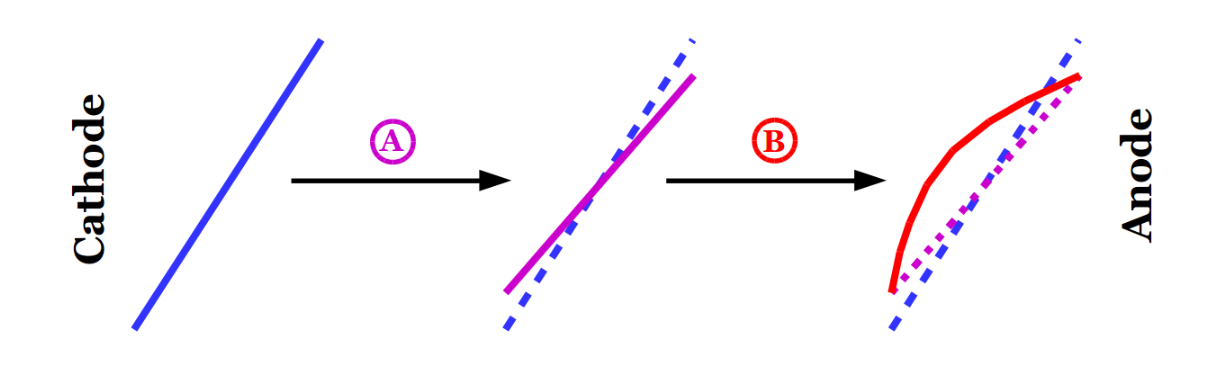
\includegraphics[width=0.8\textwidth]{SCE}
\caption[SCE]{
SCE impacts the track trajectories in two ways: causing bending away towards the detector edges, as indicated in the rotation A, and bowing towards the cathode, as indicated by transformation B.
Fig. from \cite{SCE}.
}
\label{fig:SCE}
\end{figure}
%TODO: something sounds fudgy
%Therefore, SCE worsens the spatial as well as energy resolution of a track reconstruction and consequently, particle identification.
%SBND will implement a dedicated laser calibration system \cite{}, as well as calibration using cosmics track crossing cathode and anode \cite{} to model the distorted electric field.
%Once measured, correction will be applied in the reconstruction. 

\subsection{Photons Propagation}

\subsubsection{Rayleigh Scattering}

%TODO: Check length, add group velocity/ rayleigh wavelength from Patrick's
Liquid argon is transparent to its own scintillation light, allowing emitted photons to propagate over long distances. 
As scintillation photons travel, they undergo various physical processes, including Rayleigh scattering, reflections and refractions at the boundaries of the detector material.
Rayleigh scattering, a first-order effect, involves photons elastically scattering off nuclei, altering their trajectories. 
Reflection off solid surfaces in the detector is a second-order effect. 
While these effects do not change the number of photons, they modify the paths of propagation and lengthen the travel time. 
The impact of these effects on the probability of photons reaching the PDS depends on the locations where the photons are created and their paths taken to arrive at the PDS. 
This consequently leads to a non-trivial distribution of photon arrival time at the PDS, and the travel time can range from a few to several tens of nanoseconds.
Particularly, this effect is the most impactful on the prompt component of scintillation photons.
%, which is crucial for the purpose of triggering (See Chapter \ref{}) and high-precision timing analysis (see Chapter \ref{}).
The Rayleigh scattering length $\lambda_{RS}$ for VUV photons in liquid argon has been reported to be around 50 cm \cite{rayleigh50} up to 110 cm \cite{rayleigh110}, which is comparable to the size of SBND.


\subsubsection{Absorption}
Scintillation photons can be absorbed by contaminants with a high cross-section for VUV photons, such as nitrogen \cite{photon_nitrogen} and methane \cite{photon_methane}. 
Other elements, like oxygen and water, have also been observed in commercial argon \cite{photon_commercial}. 
The total absorption of scintillation photons can be modelled as an exponential suppression of the number of photons as a function of the propagation distance, with the absorption length as a parameter (similar to Eq. \ref{eq:etime}).
The absorption rate is dependent on the Rayleigh scattering length. 
Photons with a shorter $\lambda_{RS}$ undergo longer and more indirect paths, increasing their probability of absorption before reaching the PDS.

\subsubsection{Wavelength Shifting}
\label{sec:wls}

%Scintillation photons in the VUV range are typically absorbed by detector materials without being detected. 
An enhancement method for scintillation light signals in LArTPC is wavelength shifting.
Specifically at SBND, TetraPhenyl Butadiene (TPB) is employed to shift the wavelenght of VUV photon from 128 nm to 430 nm, which falls within the visible light range.
TPB is utilised at two locations: first, it is evaporated onto the highly reflective foils located at the cathode, and second, it is coated on the optical windows of the photon detectors. 
In the former method, VUV photons arriving at the reflective foils are wavelength-shifted and reflected back towards the anode for detection.
In the latter method,  VUV photons arriving at the photon detectors are wavelength-shifted into the detectable wavelength range of the detectors.

The propagation characteristics of photons differ between the VUV and visible range.
As shown in Fig. \ref{fig:vuv_visible}, the high refractive index of liquid argon at 128 nm wavelength, approximately 1.38 \cite{lar_index}, results in a group velocity for VUV photons about twice slower than visible photons.
Moreover, the Rayleigh scattering length for VUV photons is two orders of magnitude smaller compared to visible photons.
Therefore, VUV photons are more susceptible to Rayleigh scattering and have a higher probability of absorption \cite{PatrickPhD}.
\begin{figure}[htp] 
\centering    
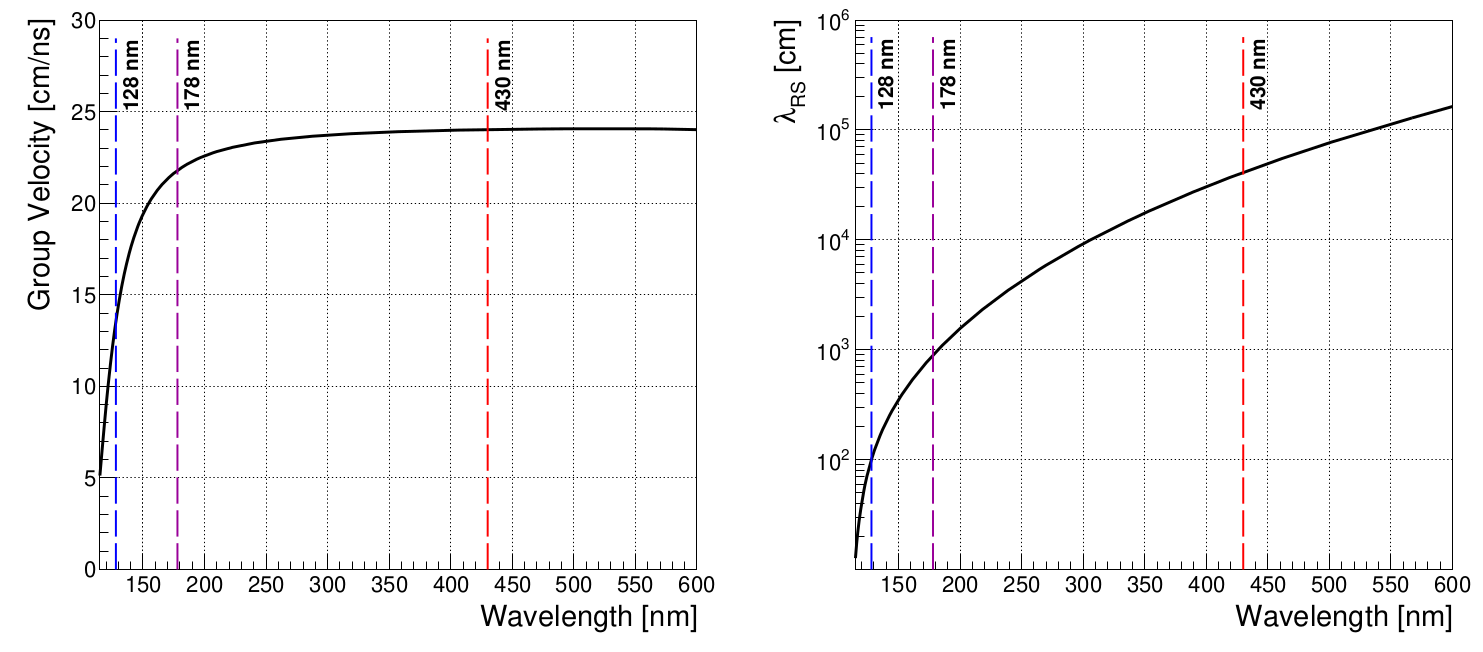
\includegraphics[width=0.85\textwidth]{vuv_visible}
\caption[vuv_visible]{
Graphs showing group velocity (left) and Rayleigh scattering (right) as a function of the wavelength of photons in liquid argon.
The lines at 128 nm, 178 nm and 430 nm are the wavelengths of scintillation photons in liquid argon, xenon-doped argon and from re-emission by wavelength-shifting by TPB. 
Fig. from \cite{PatrickPhD}.
}
\label{fig:vuv_visible}
\end{figure}
Conversely, visible photons that are reflected undergo longer propagation paths, Rayleigh scattering and propagating towards the cathode, wavelength-shifting and reflecting back the full width of the detector before reaching the photon detectors.
The spatial distribution of visible photons is more diffused and spread across a larger number of photon detectors compared to direct VUV photons \cite{PatrickPhD}.

Consequently, this leads to different arrival time and detection probability distributions for direct VUV and reflected visible photons.
The comparison of their light yield is shown in Fig. \ref{fig:light_yield_Diego} for TPB-coated and uncoated PMTs.
Closer to the anode, the light yield primarily comes from the direct VUV photons, detectable by coated PMTs.
Meanwhile, closer to the anode, and hence the reflective foils, the contribution to the light yield from reflected visible photons increased, which is detectable by both coated and uncoated PMTs.
ns.
The combined light yield from both components results in an improved overall light yield and a more uniform distribution across the drift length of the detector \cite{light_yield_Diego}.

\begin{figure}[htbp]
%TODO: Fix reference from Diego's talk to SBND PDS paper
\centering    
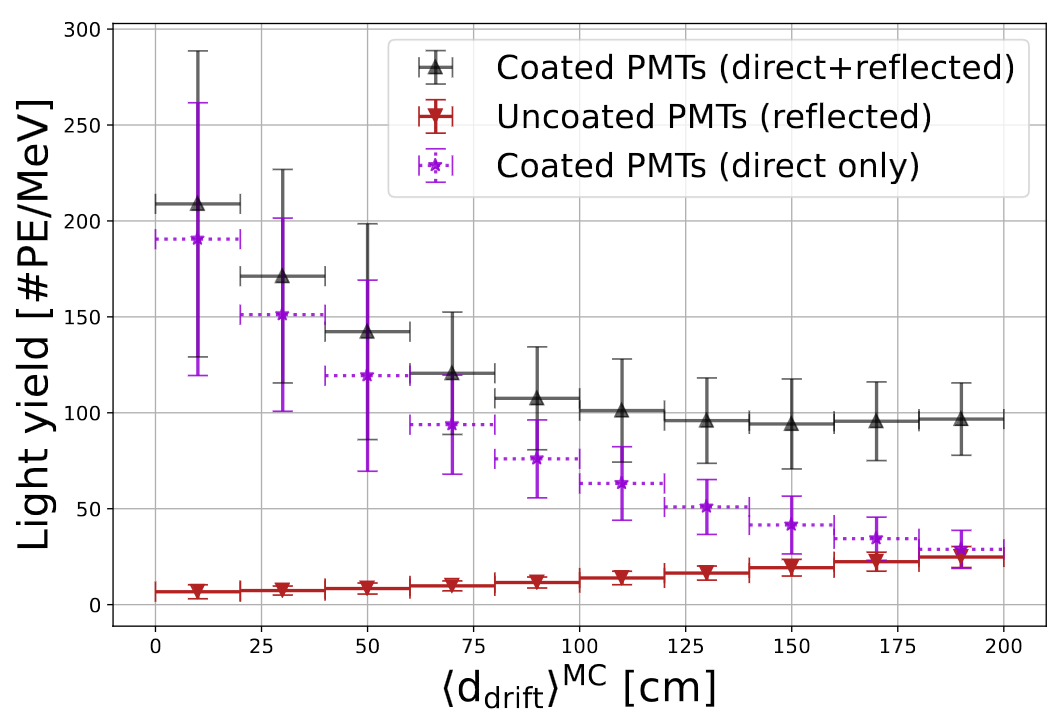
\includegraphics[width=0.55\textwidth]{light_yield_Diego}
\caption[light_yield_Diego]{
Expected light yield in SBND as a function of the mean drift distance collected by different types of PMTs.
The error bars show uncertainty due to geometrical effects of the detector.
Fig. from \cite{light_yield_Diego}.
}
\label{fig:light_yield_Diego}
\end{figure}


\section{Detection of Charge and Light}

\label{sec3:detection}

\subsection{Wire Readouts}

%TODO: add figures of signal shaping

Once arrive at the anode, the ionisation electrons induce signals on the readouts, which are typically made of three wire planes separated by a few mm as depicted in Fig. \ref{fig:LARTPC}.
A bias voltage is applied to each individual wire plane, allowing for electron transparency across the three planes.
As shown in Fig. \ref{fig:wire_current}, the drifted electrons induce bipolar signals on the two innermost planes as they pass through them; these planes are often referred to as the induction planes. 
The electrons are then collected on the outermost plane, producing a unipolar signal, and hence, this plane is commonly known as the collection plane.
The three planes are oriented 60$^{\circ}$ apart, minimising the impact of a particle travelling parallel to a wire plane.
While three-dimensional spatial reconstruction of a track requires a minimum of at least two wire planes, many modern LArTPC experiments use all three planes \cite{argoneut, icarus_det, ubooneDet, sbnd_det, protodune, dunefd_det}.
\begin{figure}[htp] 
\centering    
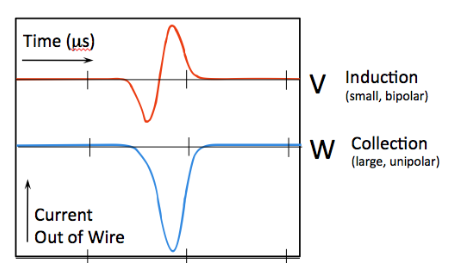
\includegraphics[width=0.57\textwidth]{wire_current}
\caption[wire_current]{
Current signals on the induction and collection wire plane, induced by a point-like charge deposition.
Fig. from \cite{argoneut}.
\hfill
\break
}
\label{fig:wire_current}
\end{figure}

The signals induced or collected on the wire planes are then shaped, amplified, and digitized by cold electronics before acquisition. 
The amount of charge collected is correlated with the energy deposited in the detector, accounting for additional corrections due to recombination and electron propagation effects as discussed in Sec. \ref{sec:recomb} and Sec. \ref{sec:edrift}. 
Finally, the spatial and calorimetry information allows for PID to be performed.


\subsection{Photomultiplier Tubes and X-ARAPUCA}

%Readout detection
Scintillation photons are detected by the Photon Detection System (PDS) located behind the wire planes, as depicted in Fig. \ref{fig:LARTPC}. 
The primary detection technology in the PDS is Photomultiplier Tubes (PMTs), which have a Quantum Efficiency (QE) of up to 30\% \cite{pmt_qe}.
However, PMTs are typically large and require sufficient volume inside the detector for installation. 
Current and future experiments are increasingly adopting Silicon Photomultipliers (SiPMs) due to their advantageous smaller size, lower power consumption, excellent signal-to-noise ratio, and a high QE of up to 40\% \cite{sipm_qe}.
The X-ARAPUCA device is a novel light collection technology utilising SiPMs, currently under development by Unicamp \cite{xarapuca} and being tested inside the SBND detector.
As shown in Fig. \ref{fig:xarapuca}, it is a light guide designed to trap light through a combination of a wavelength shifter and dichroic filters.
The dichroic filter is transparent to a narrow range of wavelengths and reflective otherwise, allowing only photons of specific wavelengths to pass through the filter and preventing their escape.
The photons are internally reflected in the trap until they are detected by the SiPMs.

\begin{figure}[htbp] 
\centering    
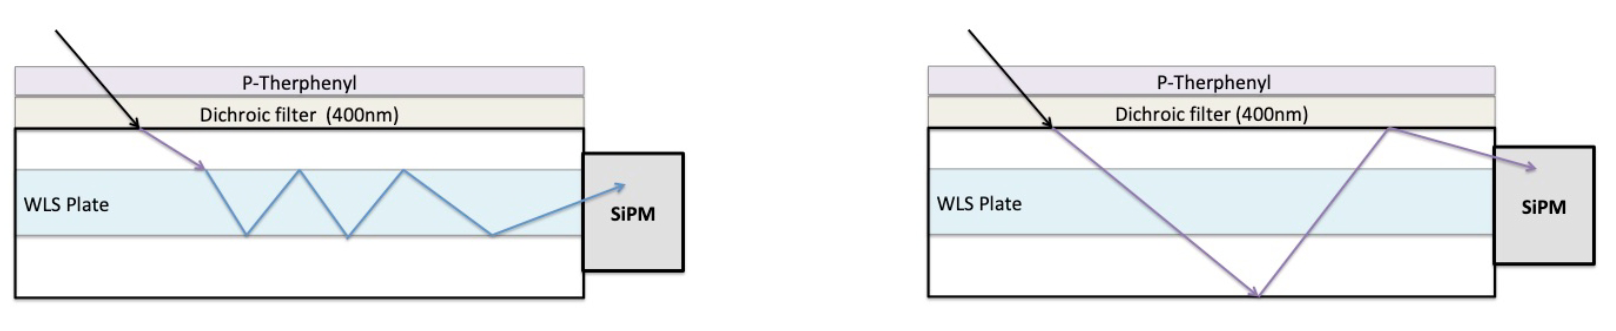
\includegraphics[width=1.0\textwidth]{xarapuca}
\caption[xarapuca]{
Diagram showing the operation principle of a X-ARAPUCA. 
The P-Therphenyl layer shifts 128 nm wavelength photons to 350 nm, allowing them to pass through the dichroic filter with a cut-off at 400 nm.
The 350 nm photons are trapped inside the reflective cavity until detected by SiPM (right).
The wavelength shifter plate converts the photons to 430 nm, trapping them by total internal reflection (left).
Fig. from \cite{xarapuca}.
\hfill
\break
}
\label{fig:xarapuca}
\end{figure}

As discussed in Sec. \ref{sec:wls}, both PMTs and X-ARAPUCAs are coated with TPB for wavelength shifting.
The re-emitted light direction is isotropic, causing coated optical detectors to suffer a 50\% reduction in efficiency due to photons emitting away from the detection surface.
TPB can also impact the detection time, as the emission of visible photons is not instantaneous.
Multiple time components of re-emitted photons from TPB have been observed, with the majority of photons re-emitted within nanoseconds and a subset re-emitted as long as a few microseconds \cite{tpb_time}.

Finally, the waveforms of the photons are digitized and acquired using a very high sampling frequency readout, ranging between 1-2 ns \cite{sbnd_det}.
This high sampling frequency gives the scintillation light signal much better timing resolution compared to the charge signal.
As a result, it provides the most precise interaction timing information available in the detector, which is particularly useful for triggering and Heavy Neutral Lepton analysis (See Chapter \ref{}).

%********************************** %First Section  **************************************
\section{Concluding Remarks}

Since the original proposal in 1977, LArTPCs have proven their potential as high precision neutrino detectors.
The understanding of particle interactions and their propagation within the detector, along with the detector's response to these particles, has significantly improved over time. 
Technological advancements in detection and readout now enable the scaling of LArTPCs from volumes of only several tons to even tens of kilotons, making them suitable for high multiplicity environments.
The next generation of LArTPCs aims to advance the field of neutrino physics, as outlined in the physics program of the SBND detector, which will be discussed in the following chapter.

%!TEX root = ../thesis.tex
%*******************************************************************************
%****************************** Third Chapter **********************************
%*******************************************************************************
\chapter{Simulation and Reconstruction}

% **************************** Define Graphics Path **************************
\ifpdf
    \graphicspath{{Chapter4/Figs/Raster/}{Chapter4/Figs/PDF/}{Chapter4/Figs/}}
\else
    \graphicspath{{Chapter4/Figs/Vector/}{Chapter4/Figs/}}
\fi

%********************************** %Opening  **************************************

Chapter 4 Opening

\newpage
%********************************** %First Section  **************************************


%!TEX root = ../thesis.tex
%*******************************************************************************
%****************************** Third Chapter **********************************
%*******************************************************************************
\chapter{Timing Performance of the Data Acquisition System}
\label{ChapterDAQ}
% **************************** Define Graphics Path **************************
\ifpdf
    \graphicspath{{Chapter5/Figs/Raster/}{Chapter5/Figs/PDF/}{Chapter5/Figs/}}
\else
    \graphicspath{{Chapter5/Figs/Vector/}{Chapter5/Figs/}}
\fi

%********************************** %Opening  **************************************
%Data Acquisition (DAQ) describes the data flow from subsystems hardware to software storage. 
%When a physics event is determined by the triggering system, the DAQ system assembles physical signals from each subsystem into an event in real-time and transports it for offline processing. 
%The DAQ system for the Short-Baseline Near Detector (SBND) must be able to handle a high data rate that arises because of the close proximity of the detector to the Booster Neutrino Beam (BNB) target, all while upholding excellent timing performance.
%Failures during the DAQ will result in meaningless physics events, and potentially irrecoverable data loss. 
%Work performed to improve the performance of the DAQ is presented, specifically on evaluating the timing information of the electronic readout for the two detection subsystems: Cosmic Ray Taggers (CRTs) and Photomultiplier Tubes (PMTs). 
%These improvements target the timing precision of each individual subsystem, as well as the timing synchronisation across multiple subsystems when running the DAQ in conjunction. 
%This is vitally important as the DAQ uses the timing information to build event with the correct signals from different subsystems.

The Data Acquisition (DAQ) system of the Short-Baseline Near Detector (SBND) plays a crucial role in building a complete physics events from various hardware subsystems using the signal timing information.
Achieving a timing precision of 1 nanosecond is a pivotal goal for the DAQ, especially important for high precision physics analysis. 
Moreover, the DAQ must be able to handle a high data rate that arises because of the close proximity of the detector to the Booster Neutrino Beam (BNB) target, all while maintaining excellent timing performance.

The work undertaken to assess the timing precision performance of the DAQ is outlined in this chapter.
An overview of the DAQ is first given in Section \ref{sec4Overview}, followed by a description of the timing reference system of the DAQ in Section \ref{sec4TimeRef}. 
The assessment of the timing performance of the Cosmic Ray Taggers (CRTs) readouts is detailed in Section \ref{sec4InternalClock}, including an evaluation of the timing resolution of the readouts and an alternative timing reconstruction employing CRT signals. 
Section \ref{sec4PMT} describes the timing performance of the Photomultiplier Tubes (PMTs) readouts, detailing on the nanosecond timing synchronisation across multiple readouts and proposing a timing correction solution to overcome the hardware limitations. 

These developments culminate in achieving the 1 nanosecond resolution and synchronisation of the CRTs and PMTs readouts in the DAQ system. 
The timing resolution of the PMTs readouts allow precise timing reconstruction of the BNB substructure, which enables identifying if an interaction occurs within a neutrino bucket. 
This sets the path way towards the high timing precision physics, such as selecting Heavy Neutral Lepton events out-of-neutrino-bucket, as discussed in Chapter \ref{ChapterSelection}. 

%********************************** %First Section  **************************************
\newpage
\section{Overview of the Data Acquisition System}
\label{sec4Overview}

%short description of daq
Data Acquisition (DAQ) is responsible for transporting data from subsystem hardware to event builder machines.
During real-time data flow, the DAQ must have the capability for event building by assembling data from each subsystem hardware into a cohesive physics event. 
Additionally, the DAQ must be able to apply complex software metrics to filter events for various data streams and data monitoring purposes.

%describe daq component
At SBND, the DAQ comprises six hardware subsystems illustrated in Fig. \ref{fig:daqOverview}.
Among these, four are the detection subsystems: the Time Projection Chamber (TPC), Photomultiplier Tubes (PMTs), X-ARAPUCAs, and Cosmic Ray Taggers (CRTs).
Each detection subsystem incorporates specialized hardware components for digitizing and reading out the physical signals. 
Moreover, two other subsystems are the Penn Trigger Board (PTB) \cite{ptb_gvs} and the SPEC-TDC. 
The PTB, as a hardware board within the SBND trigger system, is responsible to provide triggering signals to each detection subsystem independently.
The SPEC-TDC is a specialised timing mezzanine module designed specifically for timestamping purposes.
Further details about its functionality are outlined in section \ref{subsec42TimeRef}.

\begin{figure}[htbp!] 
\centering    
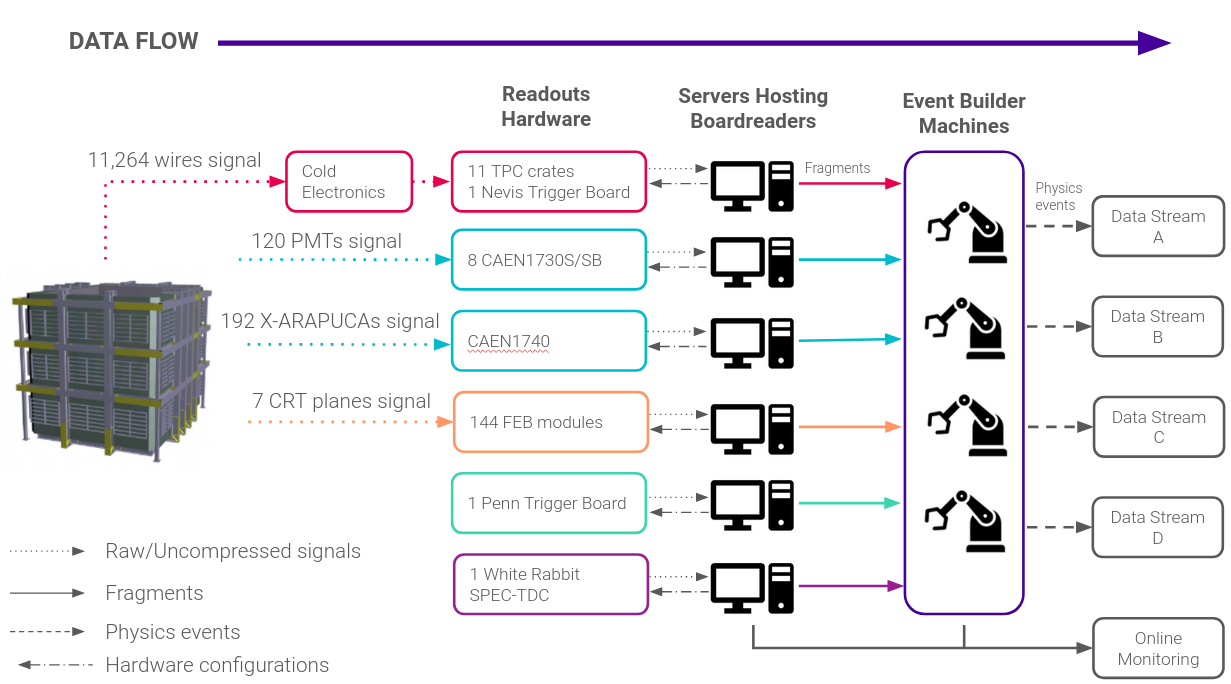
\includegraphics[width=1.0\textwidth]{DAQ_Overview}
\caption[DAQOverview]{
The DAQ system at SBND consists of six subsystems, with four dedicated to detection subsystem readouts for the TPC, CRTs, PMTs and X-ARAPUCAs, while the remaining two facilitate triggering and timing functionalities.
Each hardware component is accompanied by a corresponding software boardreader, serving as a communication bridge between the hardware and the event builder machines.
The event builders assemble a physics events and send it to different data streams for storage.
}
\label{fig:daqOverview}
\end{figure}

The DAQ software framework is provided by the \textit{artdaq Toolkit}, developed by the Real-Time Systems Engineering Department of Fermilab's Scientific Computing Division \cite{artdaq_note}.
The software acts as the backbone of the communication between the hardware components and the event builder machines.
The following section provides an overview of the DAQ workflow at SBND as illustrated in Fig. \ref{fig:daqOverview}, describing how signals are acquired from the detection hardware and subsequently digitized by boardreaders and assembled into a physics event.

%describe boardreader fragment
Within the \textit{artdaq} framework, each discrete hardware readout component has a corresponding software, known as a boardreader, facilitating communication between the readout electronics and the event builder machines.
The boardreader can send configurations directly to the hardware in one direction and retrieves data from the hardware in the opposite direction.
The data is packaged into a digitized format called a fragment as depicted in Fig. \ref{fig:fragmentDiagram}. 
The fragment class includes a header containing experiment-specific information essential for event building, an optional metadata, and a data payload storing the hardware-defined data.
A fragment is generated by the boardreader when its corresponding hardware readout receives a trigger.
The timestamp of the trigger arrival is encoded in the fragment header, which is known as the fragment timestamp.
This timestamp is the crucial value in the event building process.

\begin{figure}[htbp!] 
\centering    
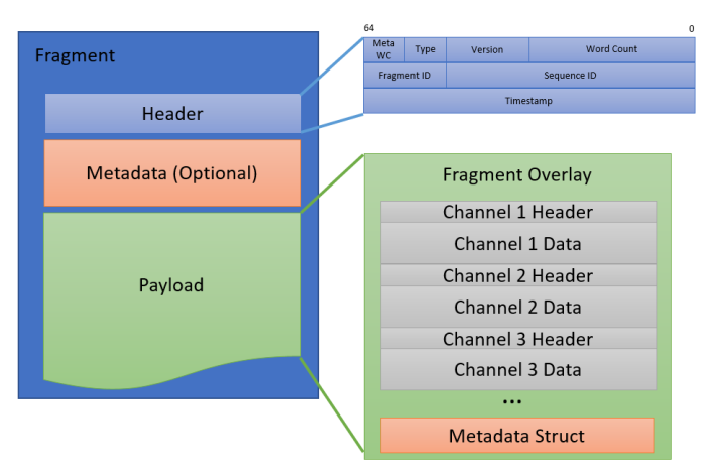
\includegraphics[width=0.6\textwidth]{Fragment_Diagram}
\caption[FragmentDiagram]{This diagram illustrates the fragment class defined by the \textit{artdaq Toolkit}. The header contains information needed for event building, of which the key information is the fragment timestamp. Optionally, the metadata structure contains hardware configurations. The payload is designated for storing data from the hardware readout, of which the data structure is pre-defined by the hardware. }
\label{fig:fragmentDiagram}
\end{figure}

%what is push/pull
Once fragments are generated, boardreaders can send them to the event builders in either one of the two configurations: push or pull. 
When operating in the push configuration, the boardreader actively sends fragments continuously at the rate at which the fragments are generated.
The sequence ID of the fragments determines the sequence ID of the built event, ensuring  that every fragment is built as a single event.
With each fragment sent, the push boardreader also creates a request message, which is multicast to all other boardreaders currently in pull mode.
This request message contains the timestamp of the push fragment. 

In contrast to the push configuration, the boardreader in the pull configuration stores the fragments in its buffer as the fragments are being generated.
These fragments are sent to the event builders only upon receiving a request message.
To determine which fragments to send, the boardreader has a configurable parameter called pull window, which specifies a time window relative to the timestamp of the request message.
The pull boardreader checks its buffer and selects the fragments with timestamps falling within this defined time window.
The selected fragments that meet the timestamp requirement are then dispatched to the event builders.
Subsequently, the event builder machines compile this set of fragments, together with one single fragment from the push boardreader that initially generated the request message, into a single event.
The sequence ID of the resulting event is determined by the push fragment.

\begin{figure}[htbp!] 
\centering    
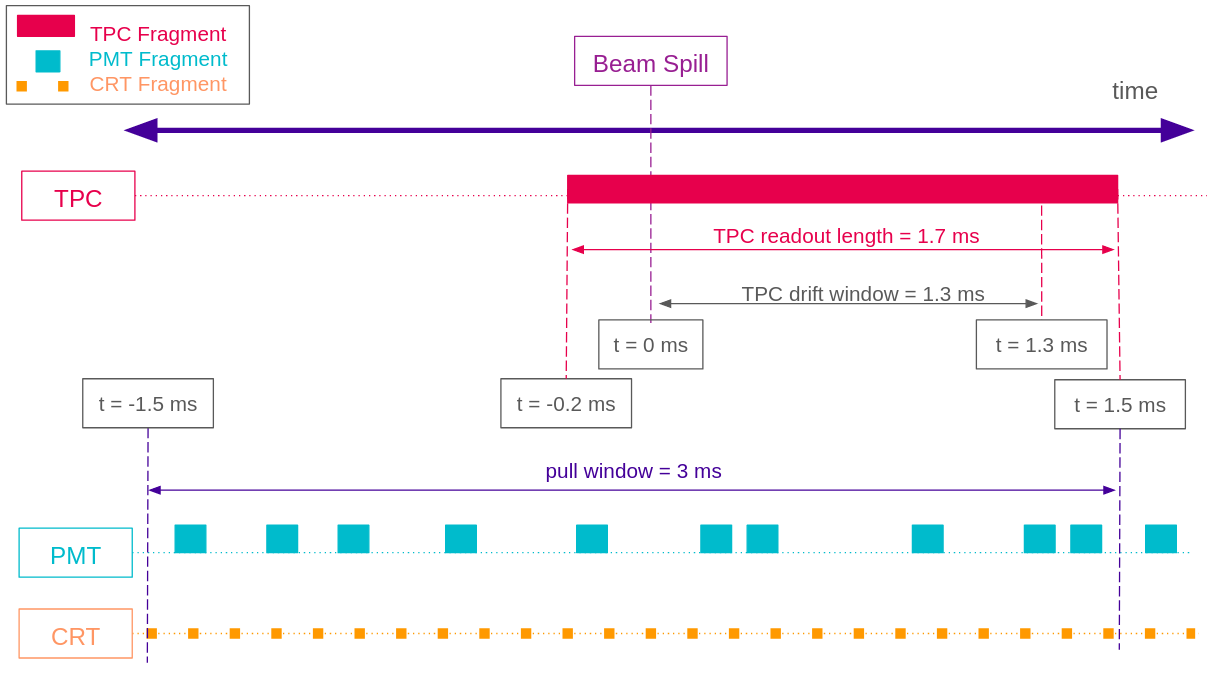
\includegraphics[width=1.0\textwidth]{SBND_Event_Structure}
\caption[SBNDEventStructure]{
This cartoon depicts a physics event structure at SBND, where the time axis is centred at 0 for when the beam spill begins. 
The event contains TPC fragments of readout length 1.7 ms to fully cover the drift window of an ionised electron from cathode to anode. 
The fragments generated by the PMTs and CRTs readouts are included 1.5 ms before and after the beam spill starts. 
The time asymmetry of the event structure is due to scintillation photon signals are produced and digitised much faster compared to electron signals.}
\label{fig:SBNDEventStructure}
\end{figure}

%describe an event structure
A physics event during at beam spill at SBND is built based on the structure shown in Fig. \ref{fig:SBNDEventStructure}, using the fragments from the three detection systems: TPC, PMTs and CRTs.
\footnote{13th November 2023: The DAQ hardware and software for the X-ARAPUCAs is under development and therefore, not be included in this thesis. }
Within this structure, there is only one push boardreader that increments the event sequence ID counter whilst the remaining boardreaders run in pull configuration.
The push boardreader is called the Nevis Trigger Board (NTB), which is a component of the hardware complex to readout the TPC data. 
The PTB sends a single Event trigger to the NTB that coincides with the start of the BNB beam spill if it determines a neutrino event occurs.
This generates a TPC fragment has a readout length of 1.7 ms, that fully covers the TPC drift length of 1.3 ms, and includes a padding of 0.2 ms before and after the drift.
The Event trigger timestamp is encoded in the NTB fragment header.

Meanwhile, the boardreaders for the PMTs and CRTs are in pull mode.
The PTB sends multiple Flash triggers to the PMTs readouts throughout the beam spill and CRTs readouts are self-triggered independently.
The fragment readout lengths from the PMTs and CRTs readouts are much shorter compared to TPC fragments, in the order of $\mu$s and ns respectively.
The pull window is defined to be 3 ms centred on the timestamp of the NTB fragment, to include PMTs and CRTs fragments generated 1.5 ms before and after the beam spill starts.
The event builders then package all the these fragments together to form a physics event.

%event asymmetry
The event structure has an asymmetry in time due to the physics characteristics of photon signals, detected by the CRTs and PMTs, and electron signals, detected by the TPC wires.
Photon signals are much faster than electron signals.
A photon produced in CRT scintillator strip takes approximate 5 ns to travel from the far end of the strip until the readouts.
A photon produced in the TPC takes maximum 15 ns to arrive at the PMTs from the scintillation location.
An ionised electron produced at the same time in the TPC takes 1.3 ms to fully drift from the cathode to the anode.
Therefore, scintillation photon signals produced during the beam spill need be digitized and readout much earlier compared to the electron signals.

%describe a data stream
After the event builder machines complete building a physics event, the resulting event can be filtered and sent to various locations for serving different downstream analysis purposes. 
This process is commonly referred to as data streaming.
The \textit{artdaq Toolkit} provides options to add customisable filtering steps in real-time, such that the event builders can apply complex software metrics based on the fragment contents of an event.
Once an event passes the filter, the event builders send it to a location defined by the filter.
If an event does not pass the filters, it will be dropped in real-time.

\begin{figure}[htbp!] 
\centering    
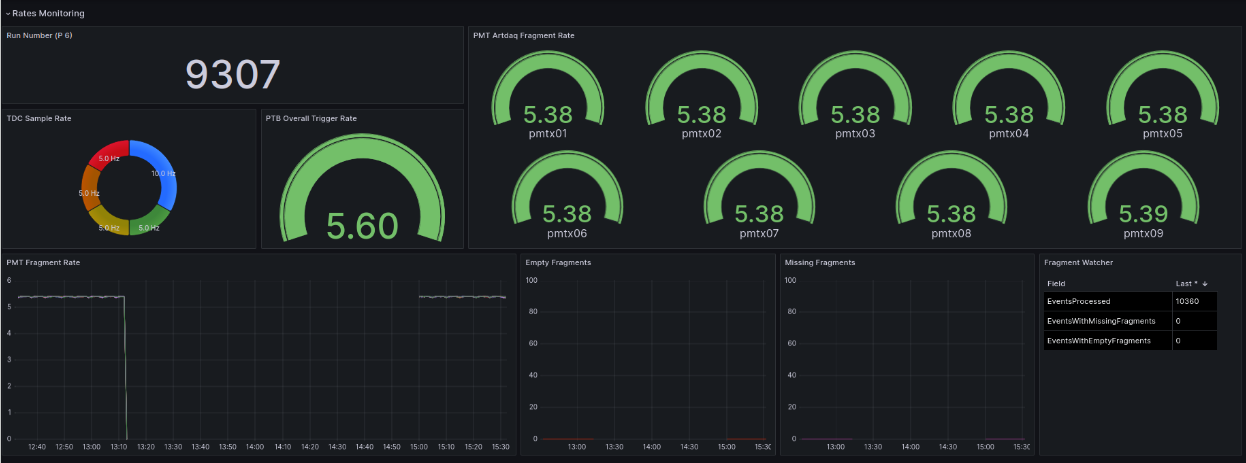
\includegraphics[width=1.0\textwidth]{Grafana}
\caption[Grafana]{
This screenshot displays a section of the Grafana monitoring website for the boardreaders of the PMT DAQ.
Some key information to quickly evaluate the status of the PMT boardreaders are shown.
For example, the fragment generation rate is expected be consistent with the trigger rate sent by the PTB whilst the empty fragment rate and the missing fragment rate stay flat at zero.
}
\label{fig:Grafana}
 \end{figure}

\begin{figure}[htbp!] 
\centering    
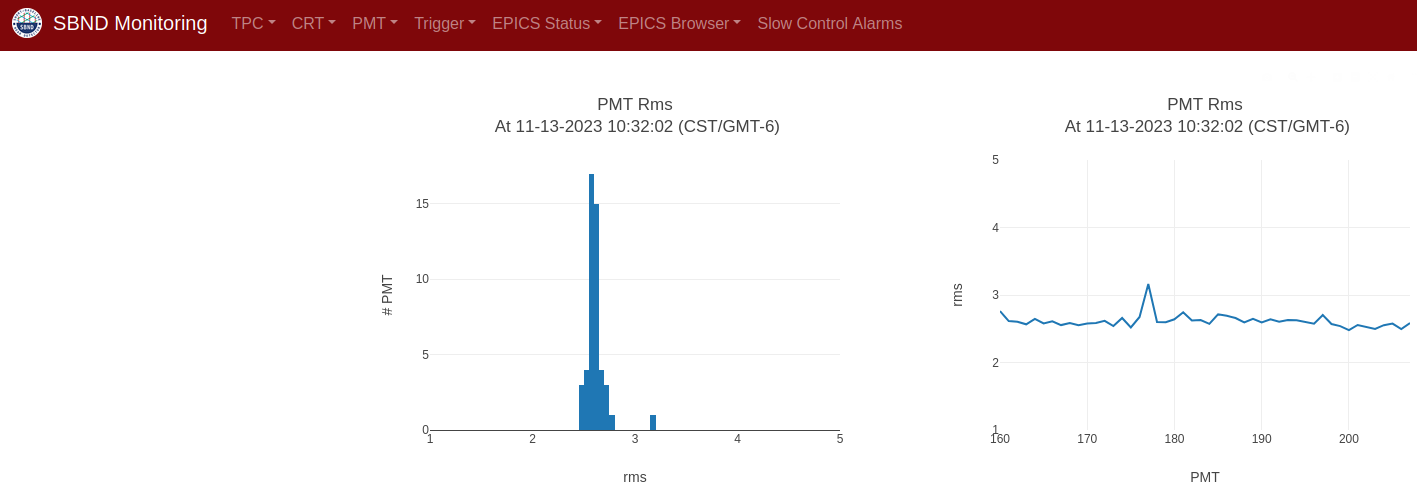
\includegraphics[width=1.0\textwidth]{Minargon}
\caption[Minargon]{
This screenshot displays a section of the Minargon monitoring website to evaluate the quality of data acquired by the PMT DAQ.
For example, a metric shown here is the waveform baseline RMS, plotted as a histogram (left) and plotted with respect to the fragment timestamp (right).
This metric provides monitoring of the baseline equalisation and stability over time.
}
\label{fig:Minargon}
\end{figure}

%data monitoring?
The \textit{artdaq Toolkit} also has a built-in process the bridges the event builder machines and online monitoring platforms.
Whilst running in real-time, fragments from boardreaders and physics events can be sent to the platforms for different monitoring purposes.
SBND currently employs two online platforms that monitors the health of the DAQ: Grafana and Minargon.
Grafana, as displayed in Fig. \ref{fig:Grafana}, provides real-time monitoring of the status of processes being run by boardreaders and event builders. 
Grafana monitoring also extends to include some status of the respective hardware component for each boardreader.
Minargon, as displayed in Fig. \ref{fig:Minargon}, provides real-time the data quality monitoring. 
This online monitoring process applies simple reconstruction and event display in order to quantitatively verify the physics characteristics of an event. 
The author has worked extensively on developing the monitoring processes for the DAQ of the PMTs on both Grafana and Minargon monitoring platforms during her PhD course. 

%********************************** %Second Section  **************************************
\section{Timing Reference System of the Data Acquisition}
\label{sec4TimeRef}

%short description of why need timing reference
The event building process of the DAQ relies entirely on timestamps from the fragment headers to construct a meaningful physics event.
Hence, it is crucial that the timestamp generated by each subsystem readout electronic is generated with a high level of precision and synchronisation.
SBND aims to achieve timing precision of the DAQ hardware and software readout components in the order of nanoseconds to fully leverage the physics capabilities.
The strategy is to utilise the White Rabbit (WR) timing system.

%description of WR timing 
The WR timing system is a collaborative project developed at the European Organisation for Nuclear Research (CERN) and is now a widely-used synchronisation solution in scientific community \cite{WR_paper}.
The WR has the capability to offer fully deterministic time transfer with sub-nanosecond accuracy over distances exceeding 80 kilometers.
The system is currently installed in both the ICARUS and SBND detector buildings.
The installation serves the dual purpose of ensuring timing precision within a single experiment as well as timing synchronisation across the two experiments. 
The application of the WR timing system at SBND for time transferring and timestamping are detailed in section \ref{subsec41TimeRef} and section \ref{subsec42TimeRef} respectively.

\subsection{Time and Frequency Transfer To Subsystems}
\label{subsec41TimeRef}

%Time Transfer Concept
The WR timing system consists of a Grandmaster WR switch that distributes time and frequency to all other WR switches within the WR network via optical fibre links.
The WR switch has dynamic calibration and thus, is a very reliable and robust delivery system.
The system ensures that the Pulse Per Second (PPS) signal, which has the frequency of 1 Hz, from all the slave WR switches in the network are aligned to the Grandmaster's PPS signal with sub-nanosecond accuracy and tens of picoseconds precision. 
Moreover, the Grandmaster WR switch installed at the SBND detector Building is connected to an atomic clock that is locked to a global navigation satellite system. 
As a result, the time and frequency distributed by the WR system are derived from the International Atomic Time (TAI) and the Coordinated Universal Time (UTC).

The Grandmaster switch currently distributes time to two independent WR switches, located at two different servers in the DAQ system.
One of the server houses several SVEC-FD modules, which are Fine Delay (FD) cards carried by Simple VME FMC Carrier (SVEC).
The SVEC-FD module is a high precision pulse generator, with 10 ps resolution and timebase accuracy of 2.5 ppm when used on a WR network.
Each module can output four independent pulses at a time.

\begin{figure}[htbp!] 
\centering    
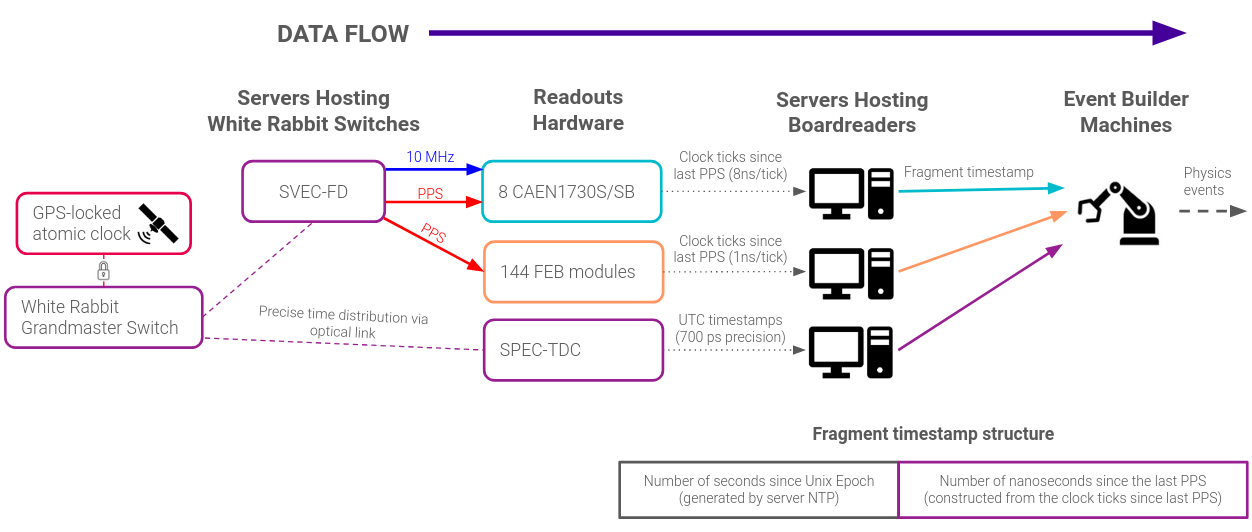
\includegraphics[width=1.0\textwidth]{time_transfer}
\caption[timeTransfer]{
This cartoon displays timing distribution from the WR Grandmaster switch to the electronic readouts for the PMTs and CRTs.
From the Grandmaster switch, the time is transferred to the SVEC-FD modules, which generates highly precise PPS signals and 10 MHz clock.
The 10 MHz clock is locked to the PPS signals such that the clock is issued on the rising edge of the PPS signal.
These frequencies are input to the electronic readouts to that produce clock ticks since the last PPS arrived.
The fragment timestamp is then generated by the boardreader using the clock ticks information, which is used by the event builders to assemble fragments into a physics event.
}
\label{fig:timeTransfer}
\end{figure}

%description of timing provided to each subsystem: PPS/ 10 MHz Clock?
The modules are used to generate clock frequencies to subsystem hardware components, which behave as the master clock that the internal clocks of the subsystem hardware can latch onto.
Since the modules are part of the WR network, the clock frequencies are synchronised with each other, and thus, so are the subsystem internal clock.
The standard clock frequency is the PPS signal and 10 MHz. 
Depends on the specification, each subsystem hardware readouts must have an input for the PPS signal, an optionally an input for the 10 MHz clock.

As illustrated in Fig. \ref{fig:timeTransfer}, this set up ensures that clock ticks generated by each electronic board is reference with respect to the last PPS arrived, and thus sharing the same time frame of reference to the PPS.
As the boardreader packages the data into fragment format, it creates the timestamp in the fragment header.
The timestamp is in UTC format and its structure consists of two parts, the second part and the nanosecond part.
The second part is the total of number of seconds since the Unix Epoch on 1st of January 1970 at UTC, which is generated by the server hosting the boardreader under the Network Time Protocol (NTP).
The nanosecond part is the number of nanosecond since the last PPS arrived, derived from the clock ticks since the PPS generated by the readout electronics.
This timestamp is subsequently used by the event builders to put the fragments together into an event.
Thus, the DAQ workflow places a vital importance on the internal clocks of each hardware readout, which are further explored in section \ref{sec4InternalClock} and section \ref{sec4PMT} for the CRTs and PMTs electronics respectively.

\subsection{Precise Timestamping}
\label{subsec42TimeRef}

%Precision Timestamp concept
%description of SPEC TDC
The Grandmaster switch is also connected to server node that hosts the SPEC-TDC module, which is short for a FMC Time to Digital Converter (TDC) carried by a Simple PCIe FMC Carrier (SPEC).
The SPEC-TDC can timestamp five input signals independently with a precision of 700 ps.
The output timestamps are in UTC standard such that it contains the last whole second in UTC format and the number of nanoseconds since the last whole second.
Thus, the timestamps are in the same time frame of reference with respect to the PPS signal.
Moreover, the SPEC-TDC also has its own boardreader so that the recorded timestamps can be built within an event, and available for downstream analysis.

% SPEC TDC 
Following Fig. \ref{fig:SPECTDC}, one application of the SPEC-TDC is to synchronise the DAQ system with respect to the beam.
This can be done by employing the SPEC-TDC to timestamp two important beam signals, that can provide status of the BNB beam.
The first one is the Booster Extraction Signal (BES), which is an early warning signalling when protons are extracted in the Booster cycles.
The second one is the Resistor Wall Monitor (RWM), which measures the instantaneous beam current onto the BNB target.
The RWM signal arrives at the SBND detector building almost simultaneously with the beam itself, and thus is used to signify when the beam arrives.
The delay between the BES and the RWM signal is approximately 333 us.
Recording the timestamps of these beam signals provides valuable tools for various monitoring purposes. 

\begin{figure}[htbp!] 
\centering    
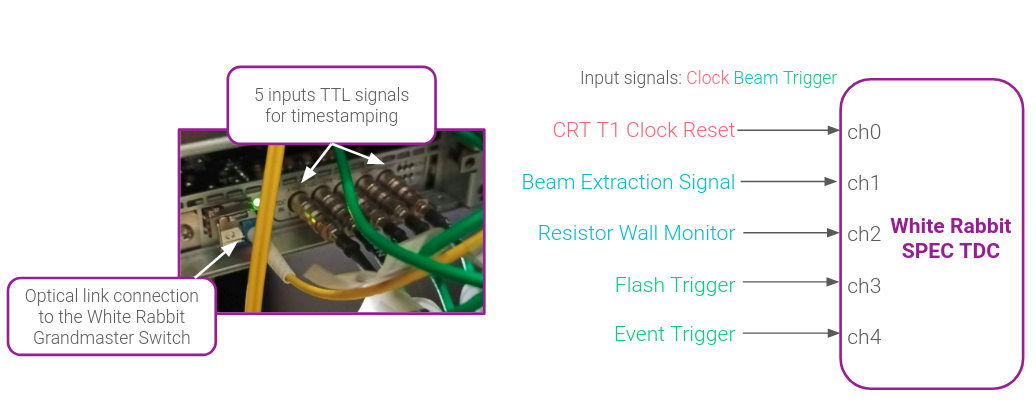
\includegraphics[width=1.0\textwidth]{SPEC_TDC}
\caption[SPECTDC]{
The photograph on the left shows the SPEC-TDC module installed at the sbnd-clk01 server.
The diagram on the right shows the input signals into the module for timestamping purposes.
}
\label{fig:SPECTDC}
\end{figure}

Additionally, the SPEC-TDC timestamps the trigger signals, which offer insights of the DAQ synchronisation with respect to the triggers. 
Referencing back to Fig. \ref{fig:daqOverview}, an event contains two types of trigger: a single Event trigger and multiple Flash triggers. 
Both types of triggers are issued relative to the beam, such that the PTB only issues triggers within the beam spill window.   
The recorded trigger timestamps can be cross referenced to the beam timestamps, and thus, enabling monitoring of the triggering synchronisation to the beam in real-time.

The last available channel of the SPEC-TDC used to record the clock reset signals for the CRT readouts. 
Upon receiving this signal, the CRT readouts reset the counters of its internal clocks.
Thus, monitoring this signal provides direct measurement of the resolution of the CRT readouts clocks.
This study was carried out by the author and is described in section \ref{sec4InternalClock}.

SPEC-TDC capabilities of high precision timestamping can be leveraged for physics application.
Recording both the timestamps of the beam and trigger signal in a single event opens up venues for various physics applications. 
One example is the characterisation of timing resolution the DAQ hardware readouts, by directly comparing the timestamps produced by the hardware against the timestamps of the SPEC-TDC given that both share the common time reference to the PPS signal.
Furthermore, it provides useful timing information for downstream analysis, for example, applying timing correction for hardware resolution and providing alternative method for event timing reconstruction. 
The SPEC-TDC applications are to be explored in the future includes nanosecond timing reconstruction, allowing for physics application such as cosmics rejection and physics searches between neutrino bucket.

The author has worked extensively on installing, testing and calibrating the SPEC-TDC over her visits at Fermilab.
The  conducted work included the hardware installations of the SPEC-TDC, by testing out two different PCIe connections on two different servers. 
One server can hold the SPEC-TDC horizontally whilst the other can hold the SPEC-TDC vertically. 
The latter was chosen due to better structural support and ventilation to host the SPEC-TDC.
The software boardreader of the SPEC-TDC also had some improvements implemented by the author, namely, better timestamp correction and higher data processing rate.
The calibration work included measuring a constant offset introduced by the SPEC-TDC hardware to be 58 ns.

%********************************** %Second Section  **************************************
\section{Timing Precision of the Cosmic Ray Tagger DAQ}
\label{sec4InternalClock}

The timing resolution of the CRT readout electronics is evaluated in the following section.
%CRT FEB
The CRT detection system consists of 7 CRT planes, and is readout by 144 Front End Board (FEB) modules \cite{crt_note}. 
A single FEB module a multifunctional board and is capable to serve 32 channels, one channel per Silicon PhotoMultiplier (SiPM). 
First it can provide a bias voltage which can be adjustable for individual SiPM as well as signal amplification and shaping.
Once the signal is shaped, the FEB can apply signal discrimination and self-triggering, such as coincidence for each pair of SiPM and coincidence across multiple FEBs.
Once the signal passes the trigger, it is digitised and timestamped with respect to the reference clock.
The data is stored in a buffer and readout via Ethernet connection.
The following section focuses on the characterisation on the timing resolution of the FEB module.

%Do I need to explain what CRT panel is made of? Or should I explain it in the detector chapter?

\subsection{Front End Board Clock}

The clock of a FEB module is a TDC unit that consists of a coarse counter of 4 ns per tick (250 MHz frequency). 
A high resolution time interpolation method is implemented within the TDC clock cycle to improve the counter to 1 ns per tick \cite{crt_clock}.
The clock resets its counter upon receiving an input reference pulse.  
The generated timestamp is the number of ticks since the clock last resets.
The FEB can also timestamp the arrival of the reference pulse and save it as special non-physics events, called clock reset event.
The timestamp of a clock reset event is essentially the counter of the clock before getting reset.

The FEB module has two internal clock counters, of which each can be reset independently via external TTL signal into LEMO connections of the module.
The first internal clock is known as the T0 clock, which is reset by the PPS signal issued by the SVEC-FD cards. 
This clock produces T0 timestamp, referencing to the PPS frame of reference.
The second internal clock is known as the T1 clock, which is reset by the BES signal\footnote{21st November 2023: At the time of writing, there is consideration to use the BES signal issued by the PTB hardware. The plan is not yet finalised}.
This signal has a higher frequency compared to the PPS signal, averaged at 5.5 Hz.
The generated T1 timestamp is expected to have a higher precision since the T1 clock is reset more frequently. 
Because of this clock system, the FEB module generates two independent timestamps, T0 and T1 with respect to the PPS and BES signal, for every recorded event.
The FEB module also records two types of clock reset event for the T0 and T1 clock.

\subsection{Evaluation of Timing Resolution}

%CRT Sharp Set Up
Over the summer of 2022, the author has travelled to Fermilab to conduct the work on evaluating the timing resolution of the FEB module.
It was conducted using a temporary set up for commissioning usage, called CRT Sharps as photographed in \ref{fig:crtSharps}.
The CRT Sharps was made of two sets of four CRT panels. 
Each set of panels was placed upstream and downstream of the SBND detector cryostat, centred on the BNB location.
The panels were readout by a total of 8 FEB modules, 4 upstream and 4 downstream.
The CRT Sharps was commissioned during the period at which the BNB beam was on. 
The triggering condition was to have signal coincidences between the upstream and downstream panels during the beam spill.
This was to ensure that CRT Sharps setup only recorded events produced by muons coming from beam neutrinos and therefore, functioned as a beam telescope.
The analysis described below used dataset recorded by the CRT Sharps during the summer and fall of 2022.

\begin{figure}[htbp!] 
\centering    
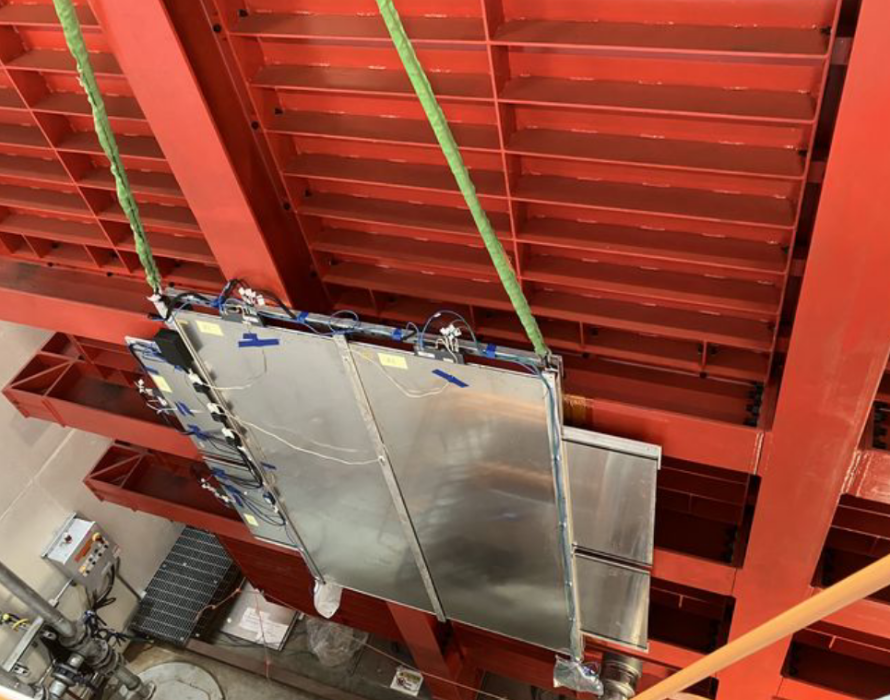
\includegraphics[width=0.6\textwidth]{crt_sharps}
\caption[crtSharps]{
The photograph shows the downstream panels of the CRT Sharps set up, hanging on the back wall of the SBND cryostat. 
The CRT Sharps was positioned precisely such that it was centred on the BNB beam.
}
\label{fig:crtSharps}
\end{figure}

%T0 Clock
%As previously described, the FEB can store the timestamps of clock reset events, which are the timestamps at which the input reference signals arrive at the FEB module.
For the T0 clock characterisation, the T0 clock reset events were of interest.
The timestamp T0 of the T0 clock reset event is the number of nanosecond since the FEB module last receives a PPS signal to reset its T0 clock.
To measure the clock variation, one can simply compare this timestamp with respect to a whole second.
An example is shown in Fig. \ref{fig:UpstreamT0StabilityCombinedBoard79} for a single FEB module numbered 79.
The T0 timestamp of the T0 clock reset event shows variation within roughly 2 ns of every second. 
The standard deviation of this timestamp distribution is the direct measurement of the T0 clock variation.
This indicates that the FEB module 79 consistently received the PPS signal to reset its T0 clock and the resolution of the T0 clock of the FEB is of the order $\mathcal{O}$(2 ns).
This measurement was repeated for other FEB modules of the CRT Sharps and the finding was consistent.

\begin{figure}[htbp!] 
\centering    
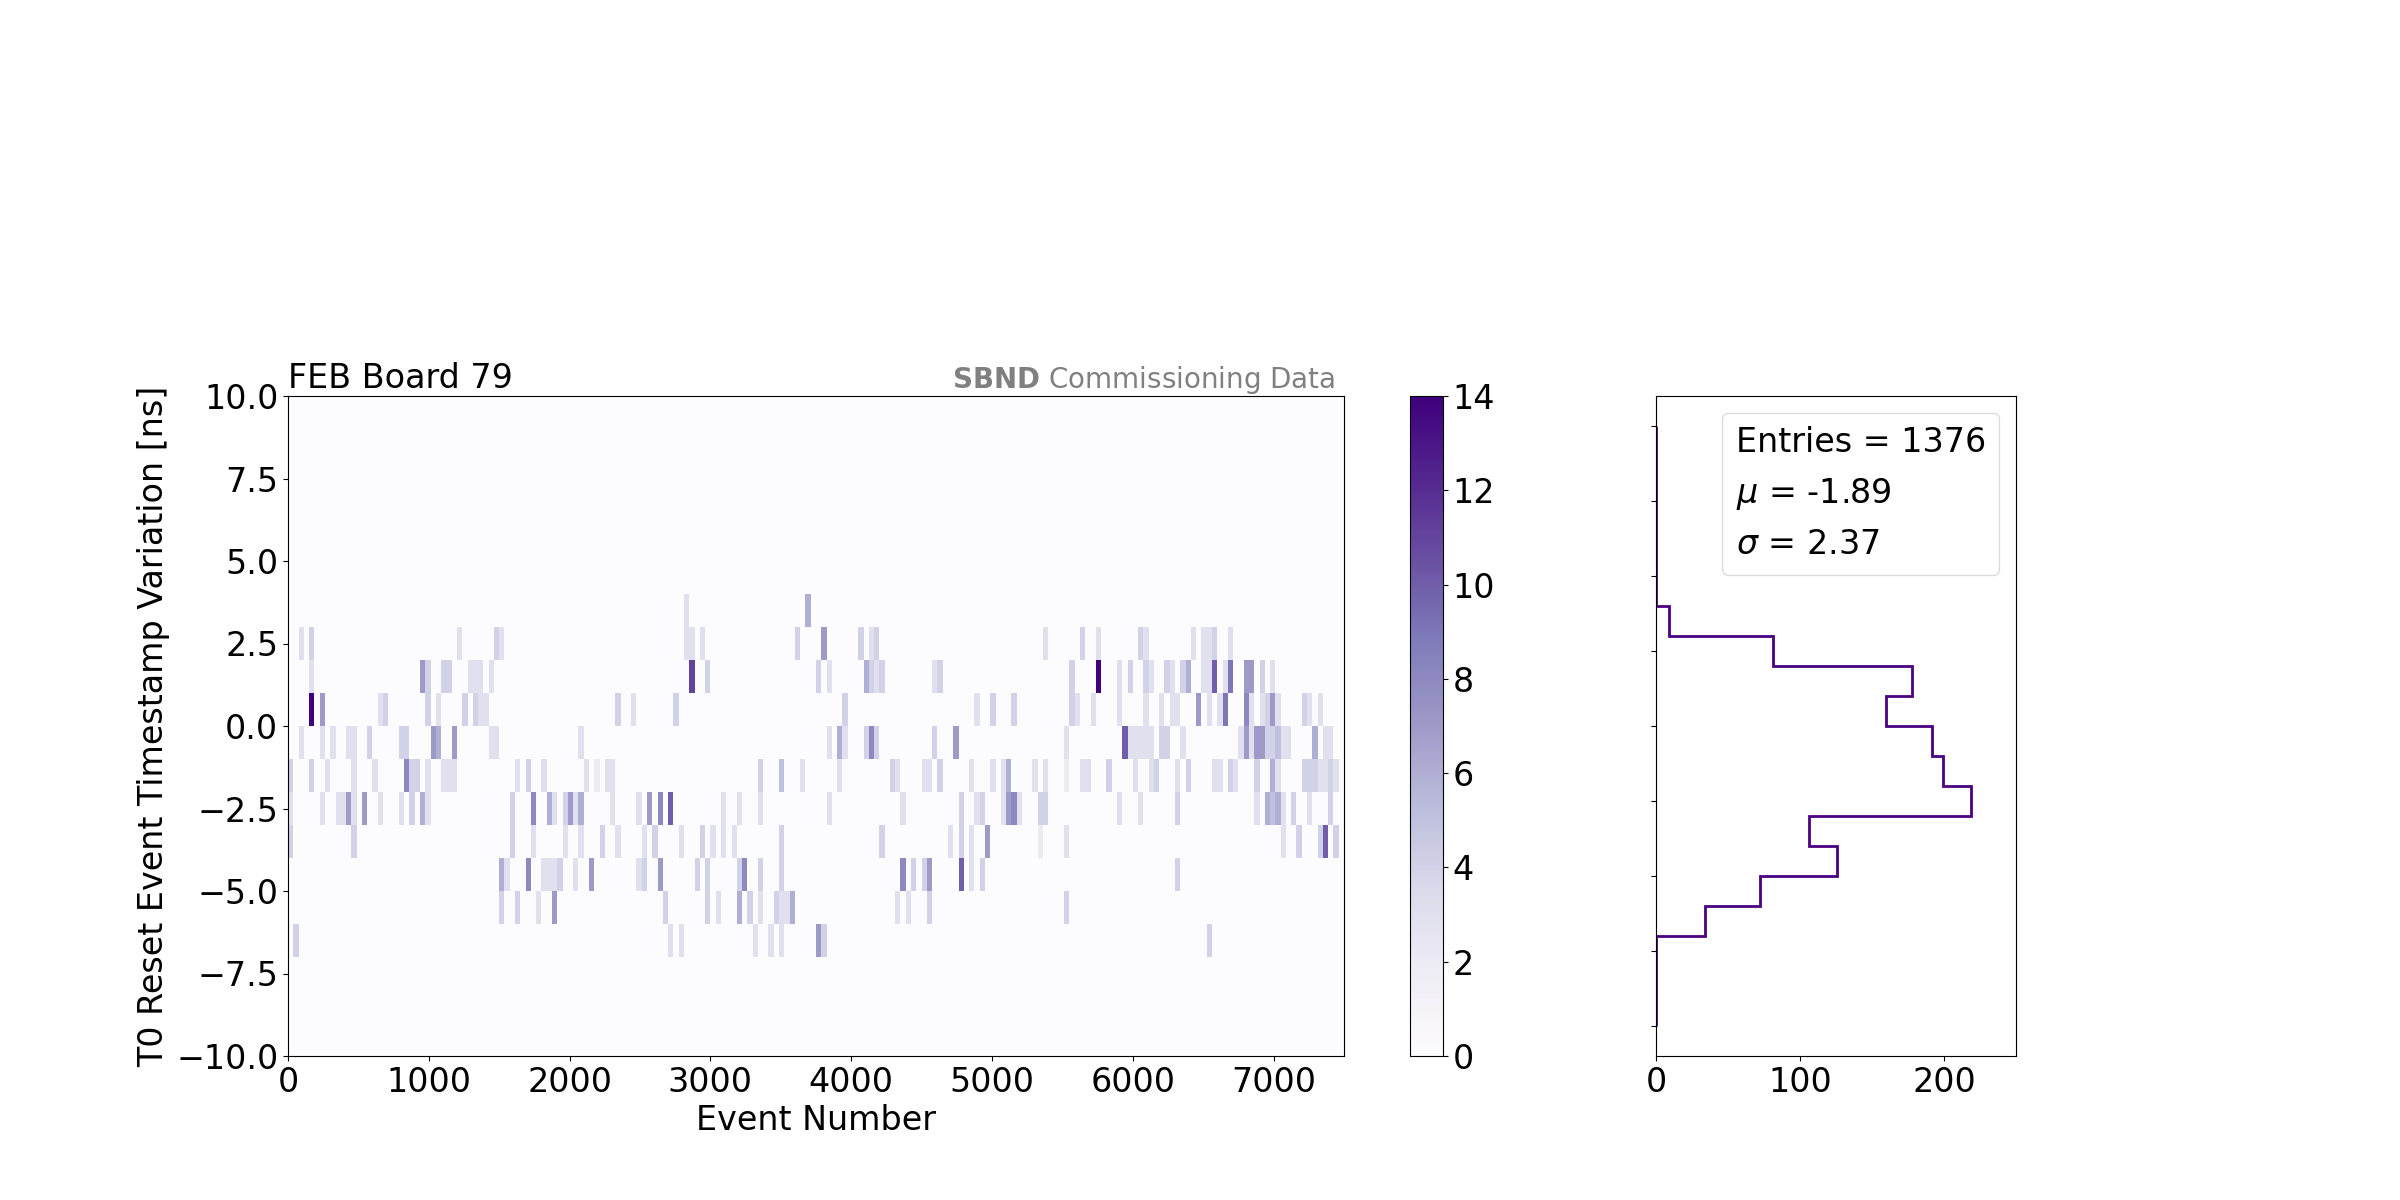
\includegraphics[width=1.0\textwidth]{upstream_T0stability_combined_board79}
\caption[UpstreamT0StabilityCombinedBoard79]{
The plots display the T0 timestamp of the T0 clock reset events with respect to a whole second. 
The timestamp variation indicates the resolution of the T0 clock, which is of the order $\mathcal{O}$(2 ns).
The left plot shows the timestamp variation with respect to the event number to check for the stability of the clock over a period time whilst the right plot is a histogram to easily check for the spread of the distribution.
}
\label{fig:UpstreamT0StabilityCombinedBoard79}
%\end{figure}

%\begin{figure}[htbp!] 
\centering    
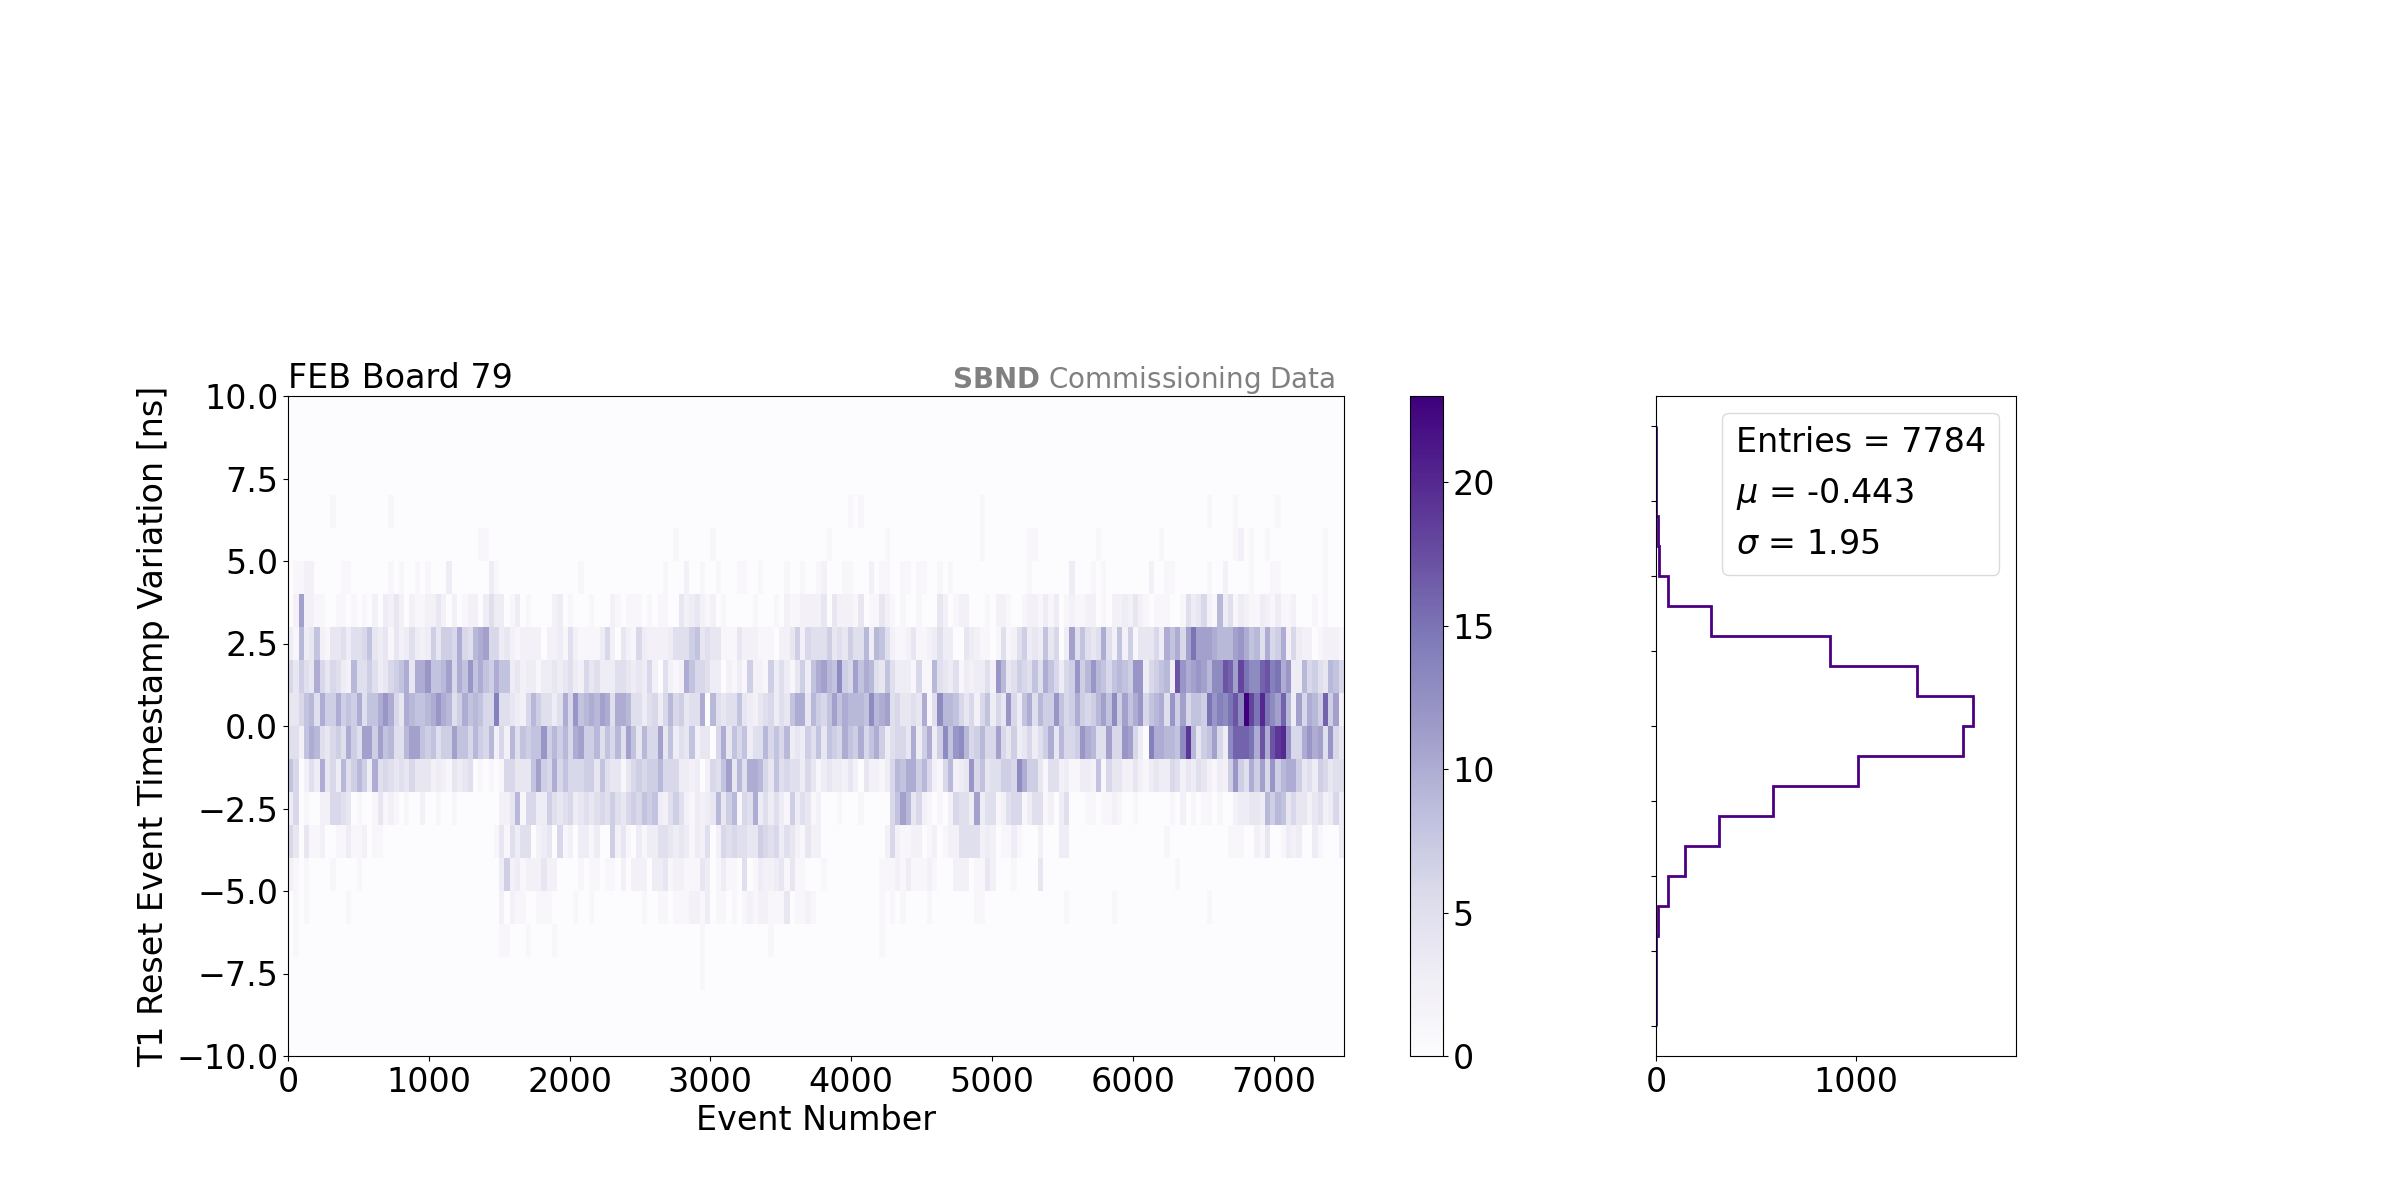
\includegraphics[width=1.0\textwidth]{upstream_T1stability_combined_board79}
\caption[UpstreamT1StabilityCombinedBoard79]{
The plots display the T0 timestamp of the T1 clock reset events, with respect to the SPEC-TDC recorded timestamp of the BES signal. 
The left plot shows that the T1 clock reset event with respect to the event number, indicating that the T1 clock was reset regularly and therefore, stable.
The right plot is a histogram of the time variation distribution, showing a standard deviation of the order $\mathcal{O}$(2 ns).
This resolution is in fact by the resolution of T0 clock given that T0 timestamps are being plotted. 
}
\label{fig:UpstreamT1StabilityCombinedBoard79}
\end{figure}

%T1 Clock 
%As shown previously, the T1 clock of the FEB module is reset by the BES signal.
Similarly for the T1 clock characterisation, the T1 clock reset events were selected and their timestamps were examined, specifically the T0 timestamps.
The timestamp variation was measured by comparing directly against the SPEC-TDC recorded timestamp of the BES signal, given that the SPEC-TDC has a higher precision than FEB internal clocks.
The cable length differences were corrected for the comparison.
%Since the SPEC-TDC is much more precise compared to the clocks of the FEB modules, comparing the T0 timestamps against the SPEC-TDC provides some insights about the clock characteristics.
The comparison is plotted in Fig. \ref{fig:UpstreamT1StabilityCombinedBoard79}, shown for a single FEB module 79.
The plot indicates that the T1 reset events arrived consistently at the FEB module and thus, its T1 clock was reset regularly.
The standard deviation of the distribution does not give direct measurement of the resolution of the T1 clock since the T0 timestamps are being examined. 
In fact, the standard deviation is smeared out by the resolution of the T0 clock, and thus, also of the order $\mathcal{O}$(2 ns).
Even though the intrinsic resolution of the T1 clock can not be directly measured, it is expected to be lower due to more frequent resets.
This measurement was also repeated for other FEB modules of the CRT Sharps and the resulting plots showed similar findings.

Moreover, the T1 clock reset events also provide an additional method to further characterise the T0 clock of the FEB module. 
This can be done by plotting the T0 timestamps variation against the T0 timestamps, as shown in Fig. \ref{fig:Board79T1Drift2d} for the FEB module numbered 79.
The plot indicates the T0 clock can drift overtime.
The T0 timestamp shows a little variation when the T0 clock counter is low, meaning that the timestamp was generated when the T0 clock recently received a PPS signal to reset.
Meanwhile, the T0 timestamp shows a larger variation when the T0 clock counter is high, meaning the timestamp was produced when T0 clock counter was close to a full second.
This illustrates that the precision of the timestamp is influenced by at which part of the cycle the clock counter is currently is in.
It is also possible that the counter can overflow and the resulting timestamps are meaningless.
When this happens, the FEB modules can flag these events and their timestamps need to be invalidated.
The clock drift behaviour is expected to be more prevalent with the T0 clocks than the T1 clocks due to lower reset frequency.

\begin{figure}[htbp!] 
\centering    
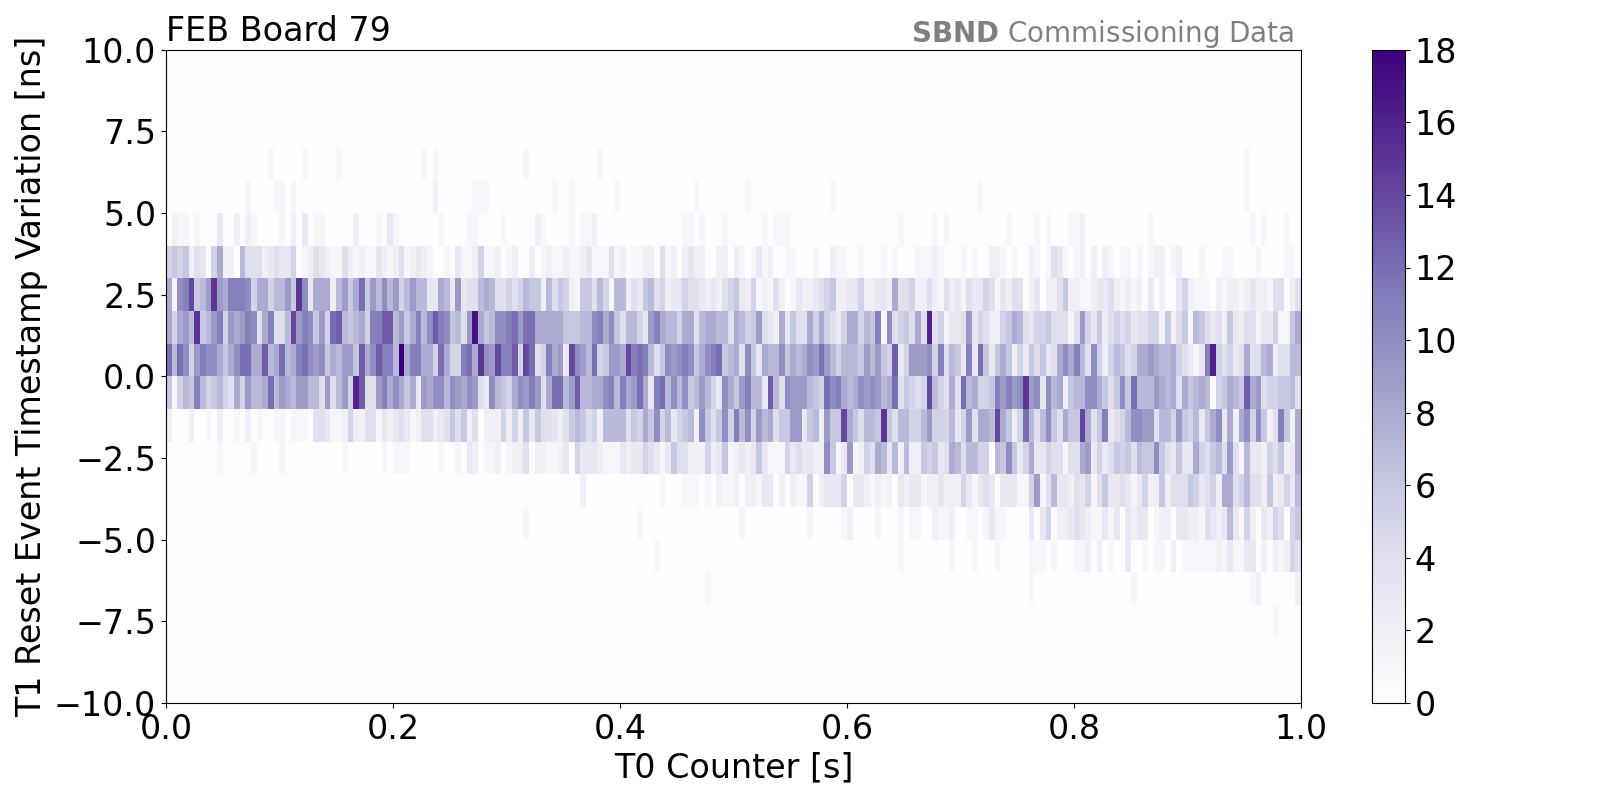
\includegraphics[width=0.70\textwidth]{board79_T1drift_2d}
\caption[Board79T1Drift2d]{
The variation of the T0 timestamp of the T1 clock reset events with respect to the SPEC-TDC recorded timestamp of the BES signal is plotted against the T0 timestamp itself.
This plot demonstrates that the T0 clock can drift such the timestamps shows a little variation at low T0 clock counter and a larger variation at high T0 clock counter.
The clock drift behaviour will be monitored in real-time during physics run to ensure clock stability.
}
\label{fig:Board79T1Drift2d}
\end{figure}

These plots are useful diagnostic tools to characterise the timing of the FEB modules: to examine whether the T0 and T1 clock resolution are stable and of the order $\mathcal{O}$(2 ns), and if the T0 clock drift can be monitored.
It is important to note that the T0 and T1 clocks of the FEB can potentially vary from run to run, and very sensitive to external noises. 
The plots have been reproduced by the CRT working group of SBND during the CRT installation periods and they will also be produced for online monitoring purposes in order to track the clock stability and resolution of the FEB modules.

\subsection{Alternative Timing Reconstruction}

%Having the SPEC-TDC also opens up opportunities for alternative timing reconstruction method. 
The following section explores how the timing information recorded by the SPEC-TDC can be used together with T0 timestamps of the FEB modules for an alternative timing reconstruction method.
The data set recorded by the CRT Sharps contained about 9000 beam events. 
The CRT 2D hit time was reconstructed from coincidental hits of 2 cross scintillator strips, and corrected for cable and propagation delay.
The CRT Hit Time T0 was reconstructed using the T0 timestamp whilst the CRT Hit T1 was reconstructed using the T1 timestamp. 
Typically, timing reconstruction from CRT data only uses the CRT Hit Time T1, whilst this following explores how the CRT Hit Time T0 can also be employed.

\begin{figure}[htbp!]
\begin{subfigure}[h]{0.49\linewidth}
\centering    
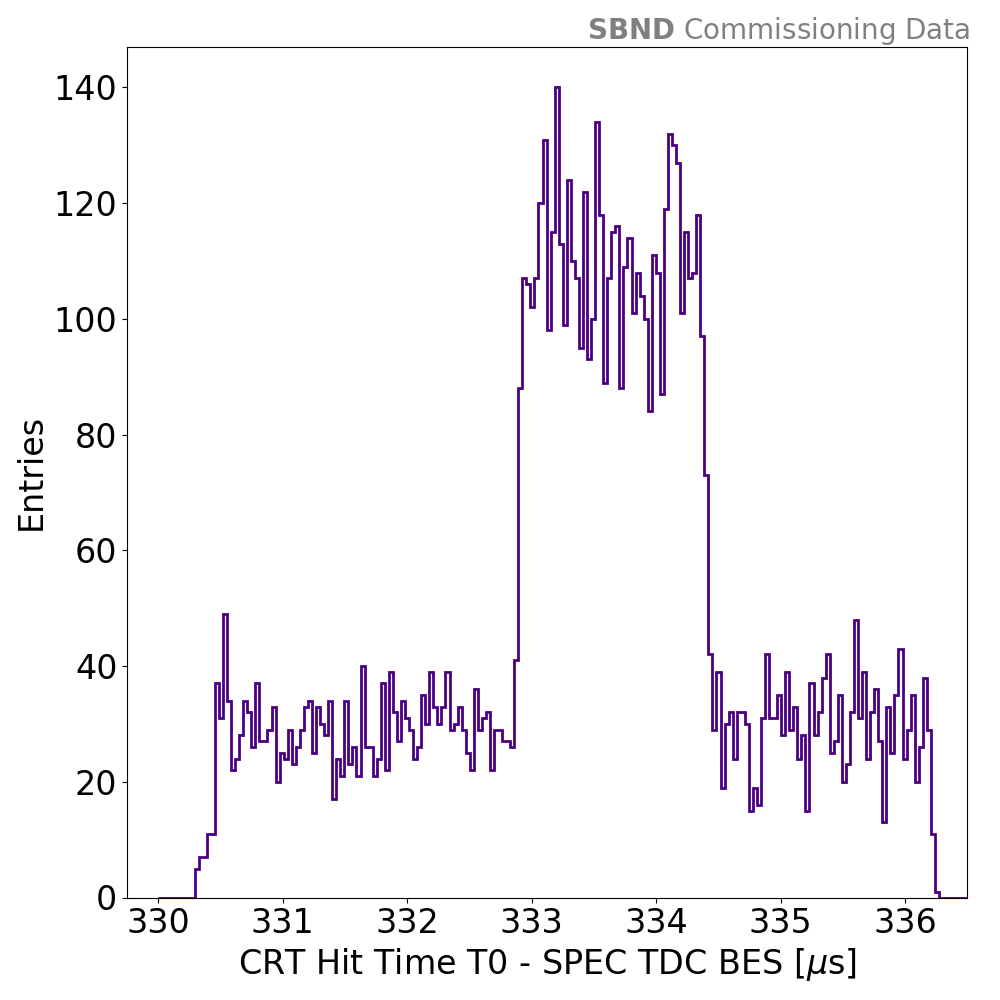
\includegraphics[width=\linewidth]{CRTT0_SPEC_TopHat}
\caption{Reconstructed using CRT Hit T0 Timestamp and SPEC-TDC Timestamp of the BES signals}
\end{subfigure}
\hfill
\begin{subfigure}[h]{0.49\linewidth}
\centering    
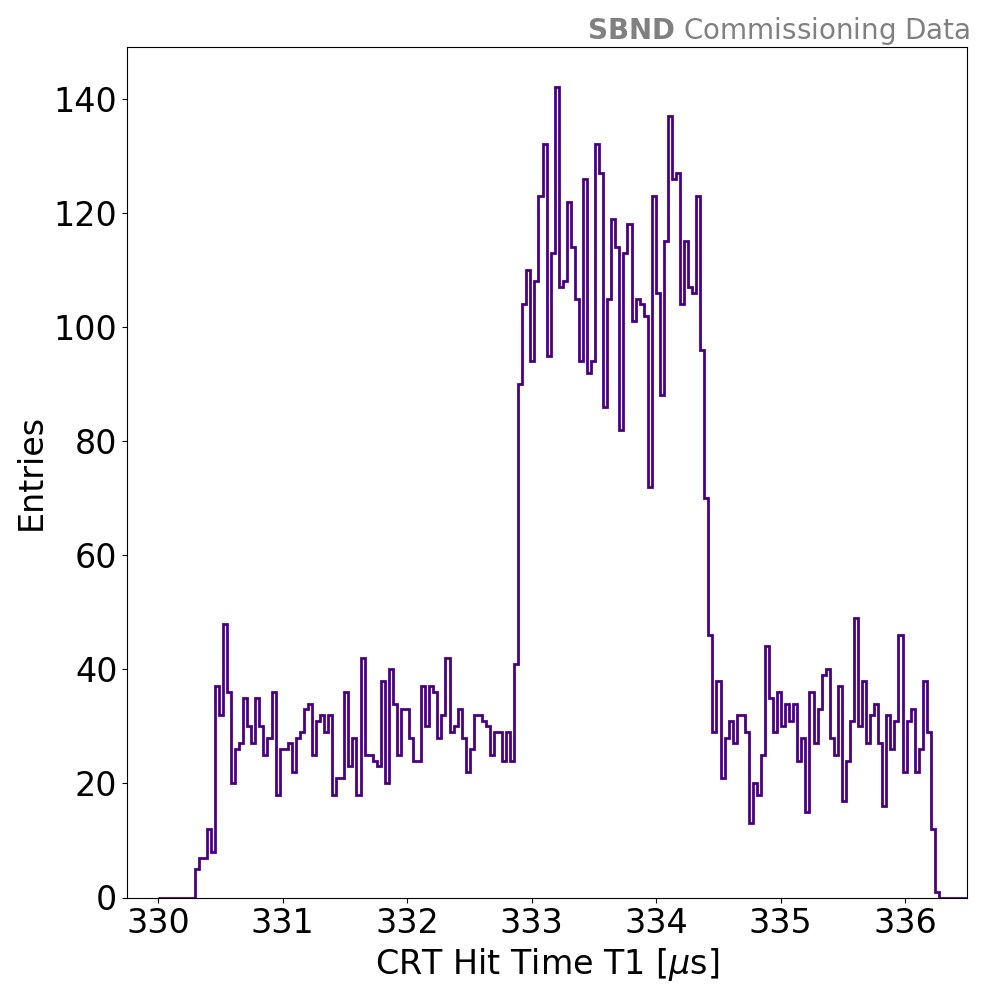
\includegraphics[width=\linewidth]{CRT_T1_TopHat}
\caption{Reconstructed using CRT Hit T1 Timestamp only}
\end{subfigure}%
\caption[topHat]{The reconstruction of the beam spill structure using CRT Hit Time T1 (left) and CRT Hit Time T0 combined with SPEC-TDC timing information (right). 
Both methods are able to reconstruct the "top hat" shape of the beam spill and show good agreement with each other.
}
\label{fig:topHat}
\end{figure}

The first timing reconstruction object is the beam spill as shown in Fig. \ref{fig:topHat} using CRT Hit Time T0 and CRT Hit Time T1 respectively.
Since the CRT Hit Time T1 is essentially the clock counter since the BES signal, the beam spill structure can be plotted directly.
The CRT Hit Time T1 plot shows that the BNB beam spill arrived 333 $\mu$s after the BES signal and lasted about 1.6 $\mu$s.
There is a clear peak at 333 $\mu$s on top of the flat distributions coming from cosmics muons, which indicates the events are indeed produced by the neutrino beam.
In the case of the CRT Hit Time T0, the frame of reference is with respect to the PPS signal, and thus, needs to be shifted relative to the beam time to reconstruct the beam spill structure.
This can be done by subtracting the BES signal timestamped the SPEC-TDC, corrected for cable lengths.
As a result, the beam spill structure can be plotted using both the CRT Hit Time T0 and the SPEC-TDC timestamps, showing a similar result.
The two reconstruction methods show good agreement with each other.
It is important to note that the beam spill structure only requires timing resolution of the order $\mathcal{O}$($\mu$s) and thus, both the CRT Hit Time T0 and T1 surpass this requirement.

\begin{figure}[htbp!]
\begin{subfigure}[h]{0.49\linewidth}
\centering    
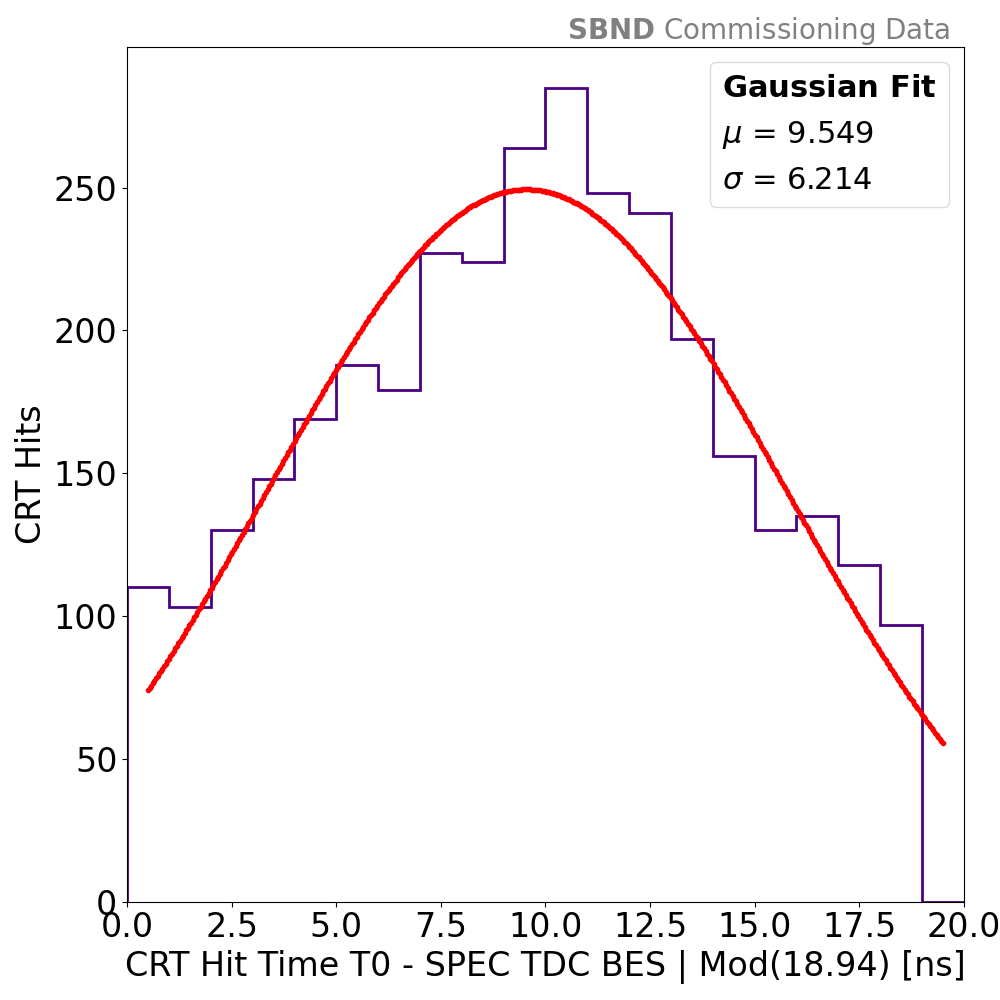
\includegraphics[width=\linewidth]{CRTT0_SPEC_Bucket}
\caption{Reconstructed using CRT Hit T0 Timestamp and SPEC-TDC Timestamp of the BES signals}
\end{subfigure}
\hfill
\begin{subfigure}[h]{0.49\linewidth}
\centering    
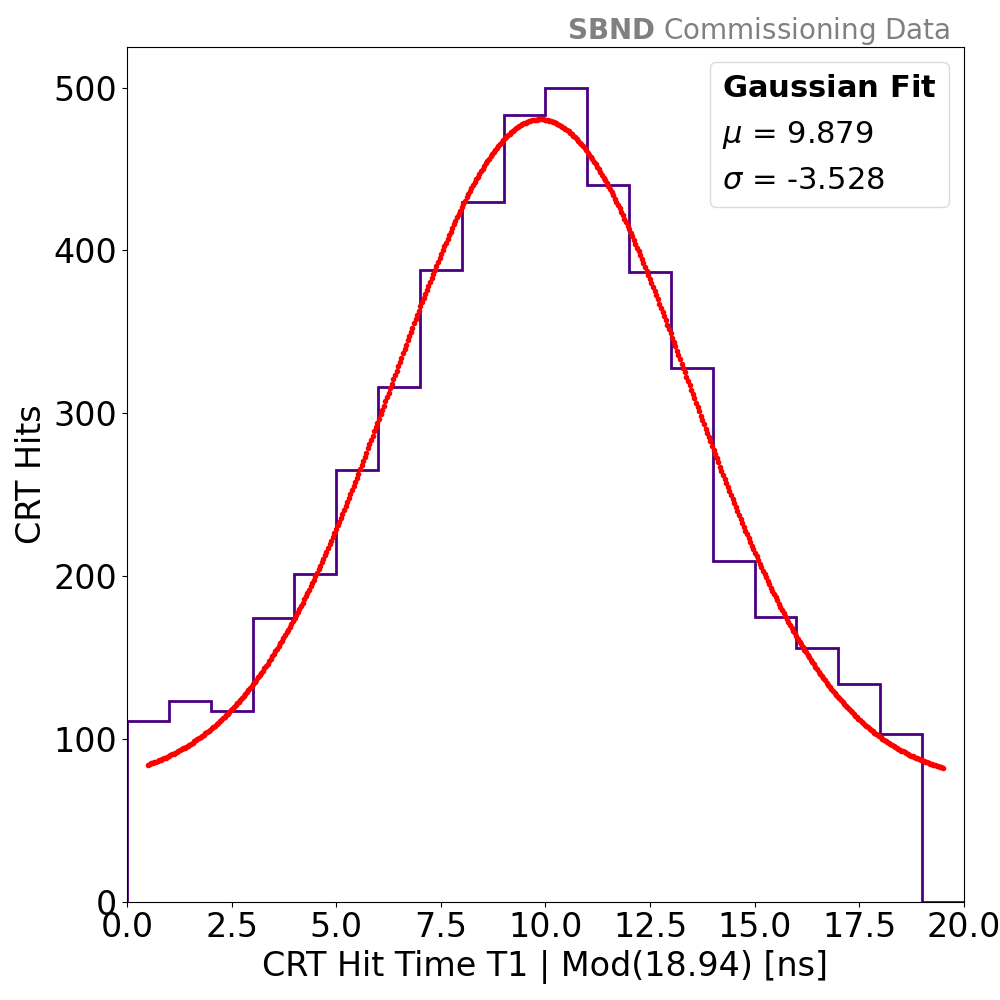
\includegraphics[width=\linewidth]{CRT_T1_Bucket}
\caption{Reconstructed using CRT Hit T1 Timestamp only}
\end{subfigure}%
\caption[beamBucket]{
}
\label{fig:beamBucket}
\end{figure}

The next step was to push the timing reconstruction further by reconstructing the substructure of the BNB beam, to determine if it is possible to resolve the beam buckets.
The BNB beam spill is made of 81 Gaussian neutrino buckets of width 1.3 ns and period of 19 ns.
Given the limited statistics of the sample to fully plot 81 buckets, the buckets were overlay on top of each other by taking the modulo of 18.94 ns of the CRT Hit Time distribution.
The period value of 18.94 ns was measured from data taken between 2017 - 2018, using CRT panels set up inside the empty SBND pit.

The resulting beam bucket plots using CRT Hit Time T1 and CRT Hit Time T0 combined with the SPEC-TDC timestamp of the BES signal are shown in Fig. \ref{fig:beamBucket}.
The CRT Hit Time T1 distribution is able to resolve the beam bucket structure precisely even with a limited statistics.
The CRT Hit Time T0 distribution can also resolve the bucket structure however with less precision. 
The Gaussian shape is more smeared out due to the intrinsic resolution of the T0 clock of the order $\mathcal{O}$(2 ns), which is larger than the width of beam bucket structure.

Whilst this alternative timing reconstruction has potential for more improvements, it shows promising outcomes at an early stage.
Specifically, this demonstrates that the CRT Hit Time T0 can be utilised for timing reconstruction purposes. 
Additionally, combining timestamps recorded by the SPEC-TDC with other hardware subsystems is a versatile tools for multiple purposes, from timing resolution characterisation to timing reconstruction.

%********************************** %Third Section  **************************************
\section{Timing Precision of the Photomultiplier Tube DAQ}
\label{sec4PMT}

%CAEN digitizer
SBND has 120 PMTs as part the Photon Detection System and they are readout by 8 CAENV1730 digitizers \cite{caen_manuals}.
The CAENV1730 digitizer is capable of recording waveforms for 16 channels independently with a sampling rate of 500 MHz.
SBND currently uses the model V1730SB which has a deeper buffer to save longer waveform as well as to handle higher data rate.
The model also offers better waveform baseline stability against temperature fluctuation.
Multiple CAEN digitizers can be synchronised to make up one complex system, such that they all behave as a single digitizer.
Thus, the following section evaluates the timing precision of CAEN digitizer by characterising the synchronisation across multiple digitizers.

\subsection{CAEN Digitizer Clock}
\label{subsec41PMT}
%clock of a single digitizer
The clock distribution of the CAEN digitizer is made up of two clock domains in the hardware: OSC-CLK and REF-CLK.
The OSC-CLK is a fixed internal oscillator that has a frequency of 50 MHz. 
This clock is responsible for handling communication between the motherboard and the mezzanines such as local bus, universal serial bus and optical link.
The REF-CLK handles sampling and triggering frequency via a clock chain.
The source of the REF-CLK can either be internal or external.
For internal mode, the REF-CLK is referenced to the OSC-CLK of frequency 50 MHz.
For external mode, the REF-CLK is fed by an external frequency via the CLK-IN connector. 

%What are the clocks
The REF-CLK is the clock of interest to ensure synchronous sampling and triggering rate, and thus the timing precision of the CAEN digitizers.
The REF-CLK frequency serves as an input to a phase-locked-loop and clock distribution device AD9510, generating three types of frequencies: the ADC sampling clock, the trigger logic clock and the output clock via the CLK-OUT connector.
The ADC sampling frequency, set as 500 MHz, handles the sampling rate of waveforms and therefore, the tick value of recorded waveforms is 2 ns. 
The trigger clock operates at 125 MHz and is responsible for handling the triggering and synchronisation logic.
For every waveform recorded, it generates a timestamp object associated with the waveform, called Trigger Time Tag (TTT)
This timestamp is equivalent to the number of ticks since the trigger clock last resets, where each tick is 8 ns.
The trigger clock is read every two clock cycles, potentially introducing fluctuations up to 16 ns.
The third clock is a frequency that is output via the CLK-OUT connector and can be propagated to another CAEN digitizer for synchronisation purpose.
This frequency is programmable, with the standard configuration set as 62.5 MHz, which the frequency value in phase with both the sampling and trigger clocks.
The AD9510 device must be programmed for a specific input frequency to the REF-CLK, to ensure that the frequencies of the sampling, the trigger and the output clock is locked in phase with the input.

%What are input to the clocks
At SBND, the CAEN digitizers are configured to use an external clock fed to the REF-CLK, such that their internal clocks are referenced to the WR timing system. 
Each CAEN Digitizer receives two external inputs: one is the PPS signal that is input into the S-IN connector, and the other is an external frequency that goes to the CLK-IN connector.
The PPS signal resets the counter of the trigger clock, such that the generated TTT value is with respect to the PPS signal.
The frequency input to the CLK-IN connector varies based on the clock synchronisation scheme. 
It can be either from the SVEC-FD modules, which make the standard 10 MHz clock, or can be from another CAEN digitizer CLK-OUT, which make the standard 62.5 MHz frequency.

%clock synchronisation
As previously stated, multiple CAEN digitizers can be synchronised. 
This can be achieved through two different clock synchronisation schemes: fan out mode or daisy chain mode as shown in Fig. \ref{fig:clockScheme}.
In fan out mode, each individual digitizer is input with the same 10 MHz clock.
The 10 MHz clock is produced by the SVEC-FD card, input to an LVDS fan out, and then into the CLK-IN connector of each digitizer.
In this configuration, every CAEN digitizer should receive identical external frequency for the REF-CLK that generates the sampling and trigger clock.
In daisy chain mode, the first digitizer in the daisy chain receives the 10 MHz clock, known as the master clock.
Its clock is then propagated to the next digitizer in the chain, known as the slave clock.
The master clock can be precisely programmed with a delay to account for cable lengths, ensuring that the master and slave clocks are in phase with each other.
The clock propagation continues from one digitizer to the next digitizer in the chain, until the last digitizer in the chain is in the same clock phase as the first digitizer in the chain.  

\begin{figure}[htbp!]
\begin{subfigure}[h]{0.49\linewidth}
\centering    
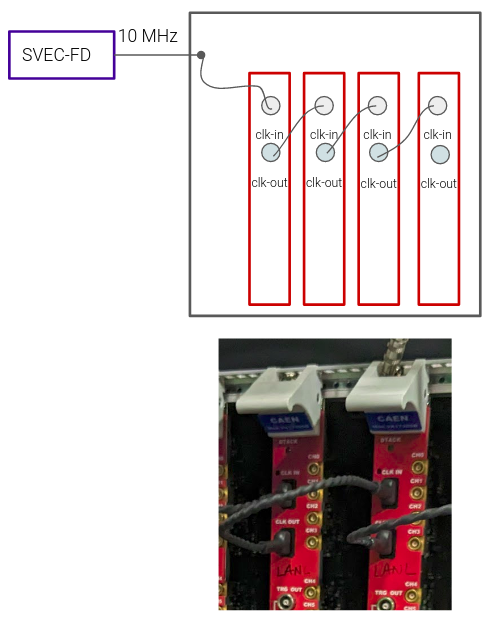
\includegraphics[width=\linewidth]{daisychain}
\caption{Daisy Chain}
\end{subfigure}
\hfill
\begin{subfigure}[h]{0.49\linewidth}
\centering    
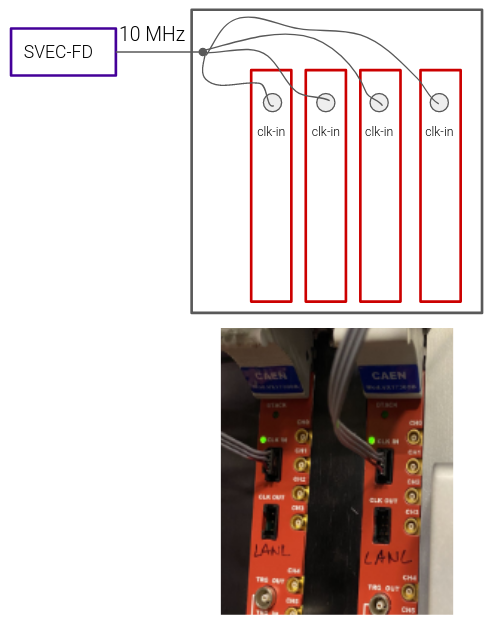
\includegraphics[width=\linewidth]{fanout}
\caption{Fan Out}
\end{subfigure}%
\caption[clockScheme]{
This diagram illustrates two different synchronisation clock schemes for the CAEN digitizers, daisy chain (left) and fan out (right).
}
\label{fig:clockScheme}
\end{figure}

\subsection{Evaluation of Timing Synchronisation}
\label{subsec42PMT}
Over the summer of 2023, the author has travelled to Fermilab for the second time to conduct the work on evaluating the timing resolution and synchronisation of the CAEN digitizers.
The first task was to determine which clock scheme to be used for physics run. 
The goal was to achieve synchronisation across all 8 CAEN digitizers and with respect the timing system of the DAQ.

%set up
The set up for the study consisted of 8 CAEN digitizers located in the same VME crate. 
Each digitizer received an identical signal into the TRG-IN connector directly from the PTB board, with the same cable length such that every digitizer was triggered simultaneously.
The trigger rate was set as 1 Hz.
To evaluate metric whether the CAEN digitizers are synchronised with each other, the timestamps of every triggered event from every digitizer should be identical with respect to each other. 

The trigger signal was also input to the SPEC-TDC for timestamping.
Timestamps of the trigger recorded by the CAEN digitizers and the SPEC-TDC can be compared against each other since both are referenced to the PPS signal.
The SPEC-TDC offers a higher level of precision compared to the CAEN digitizer.
Therefore, the comparison helps characterising the resolution of the timestamps produced the CAEN digitizer. 
This comparison also evaluates whether each CAEN digitizer is synchronised with respect to the PPS signal.

\begin{figure}[htbp!] 
\centering    
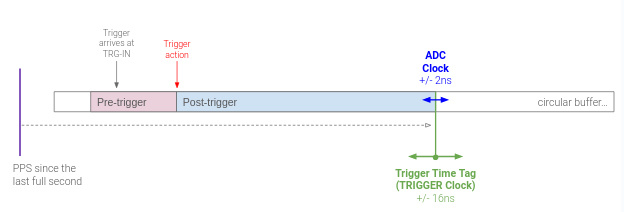
\includegraphics[width=1.0\textwidth]{TTT_diagram}
\caption[TTTDiagram]{
The diagram illustrate the how the CAEN digitizer constructs a Trigger Time Tag object upon receiving a trigger.
The timestamp embedded in the Trigger Time Tag accounts for a fixed buffer time the digitizer takes to generate the Trigger Time Tag upon receiving a trigger.
This timestamp also points the end the recorded waveform.
}
\label{fig:TTTDiagram}
\end{figure}

%CAEN Timestamp
In the previous section, the timestamps generated by the FEB module only needed adjustedment for cable lengths before being compared against the SPEC-TDC timestamps, since both the FEB modules and SPEC-TDC instantaneously generate timestamps upon receiving a trigger.
Meanwhile, the CAEN digitizer generates a timestamp object called TTT associated with every trigger, and this timestamp is not instantaneous upon the trigger arrival time, as illustrated in Fig. \ref{fig:TTTDiagram}. 
Upon receiving a trigger at the TRG-IN connector, the digitizer has a fixed buffer time before the trigger action occurs and generates a TTT.
The generated TTT also points to the end of the waveform, such that it is the timestamp value of the last tick on the waveform.
Therefore, to ensure consistency in comparing the timestamps of the CAEN digitizer and the SPEC-TDC, they need to be corrected to the same reference frame, which was chosen to be the time at which the trigger leaves the PTB front face.
If both the CAEN digitizers and the SPEC-TDC synchronised with each other, the difference in the timestamps should be 0.

\begin{figure}[htbp!]
\begin{subfigure}[h]{1.00\linewidth}
\centering    
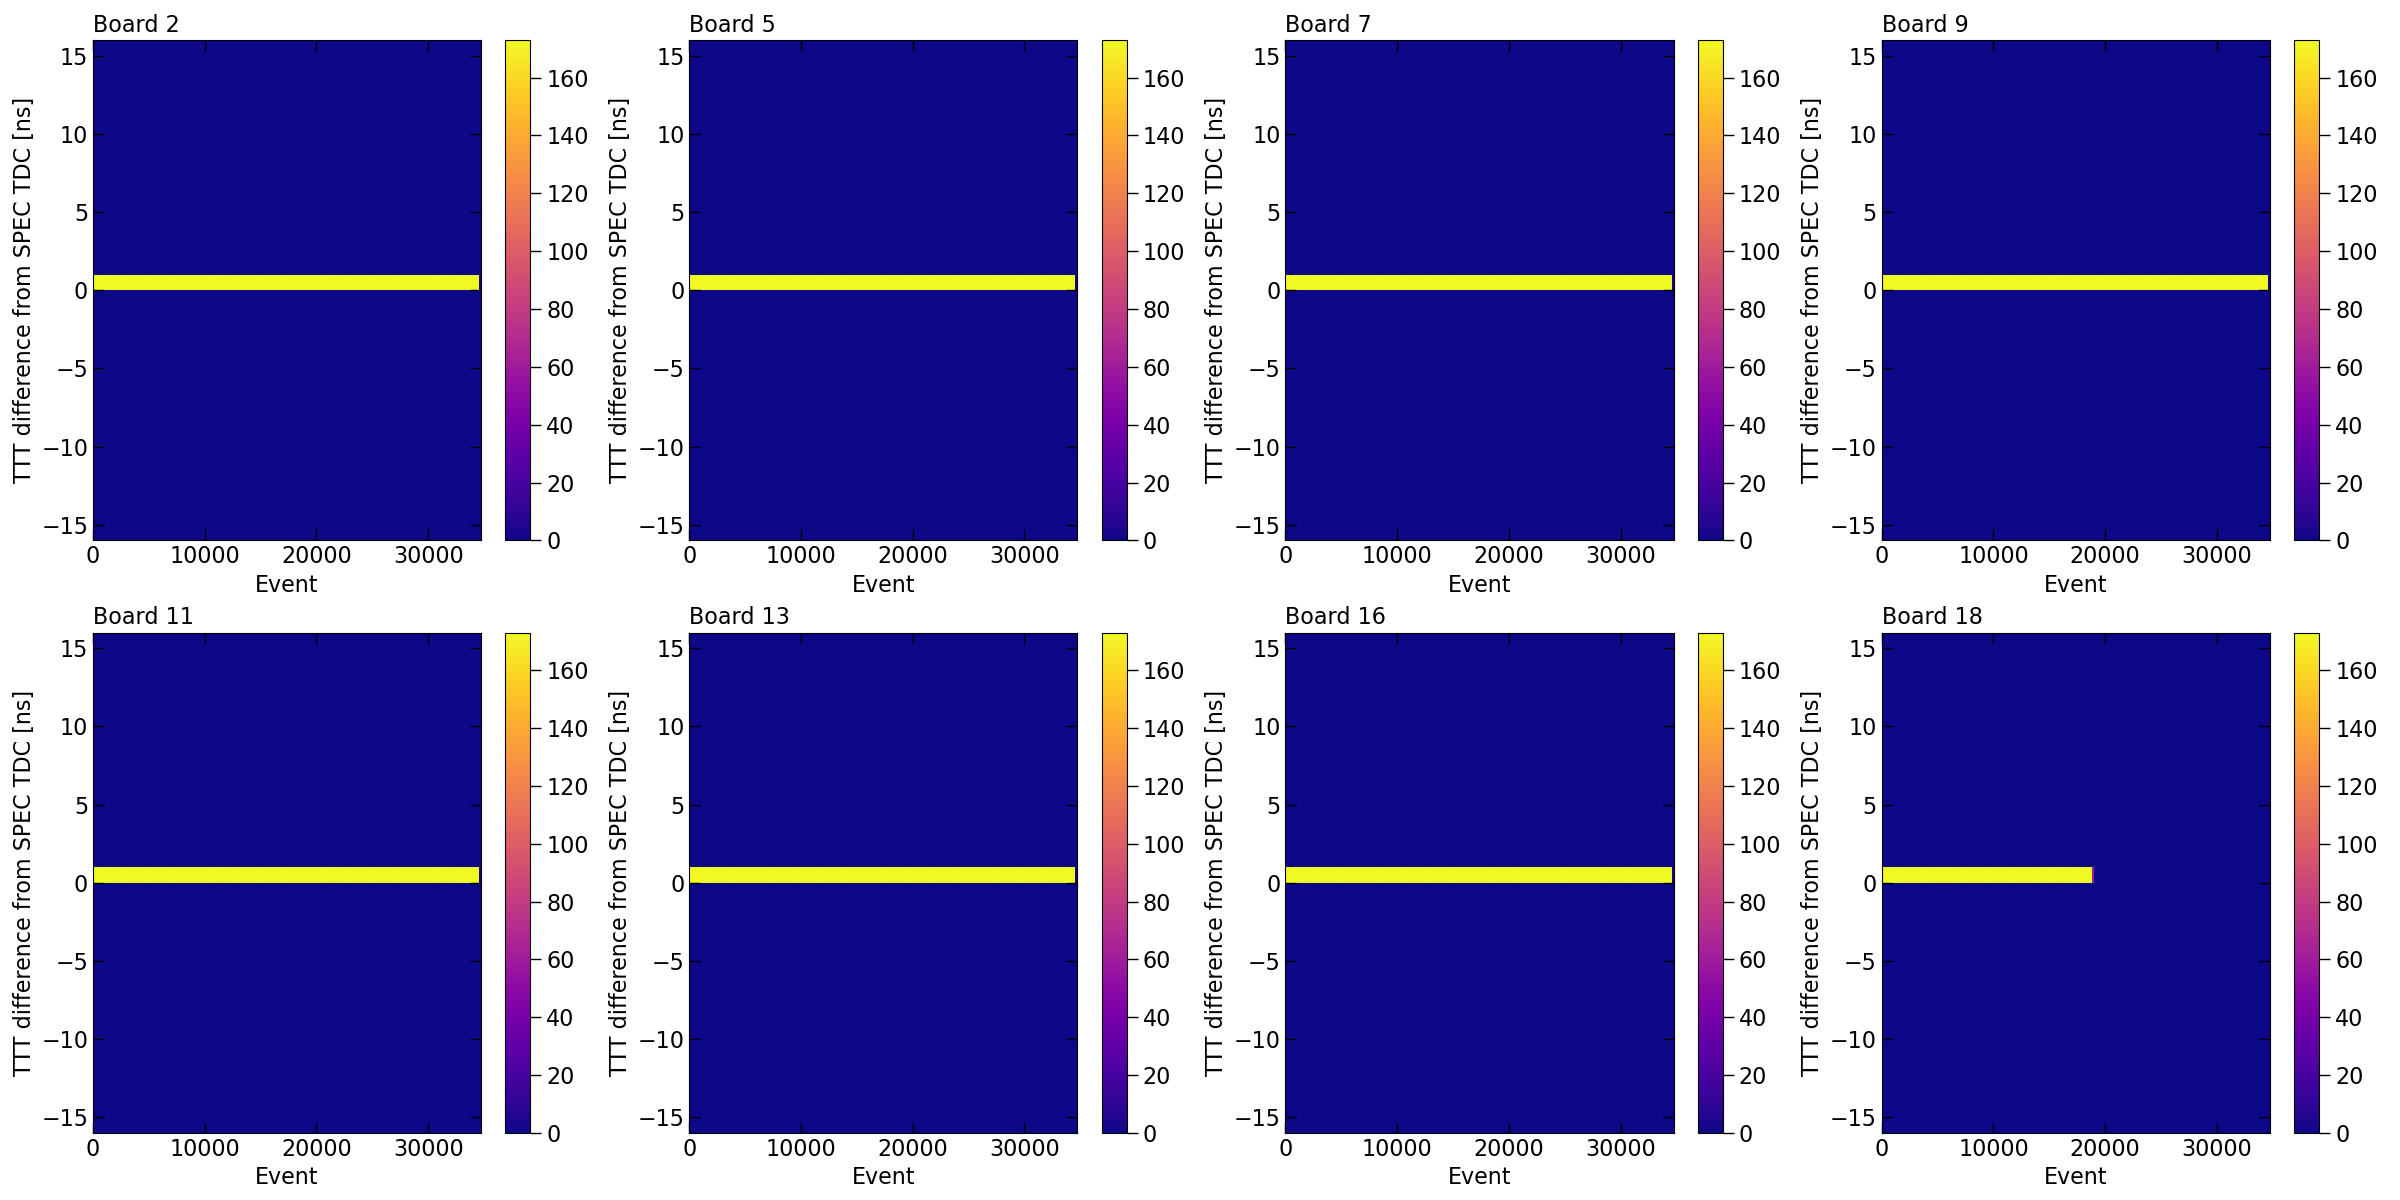
\includegraphics[width=\linewidth]{TTT_SPEC_diff_run7980}
\caption{Run7980}
\end{subfigure}
\hfill
\begin{subfigure}[h]{1.00\linewidth}
\centering    
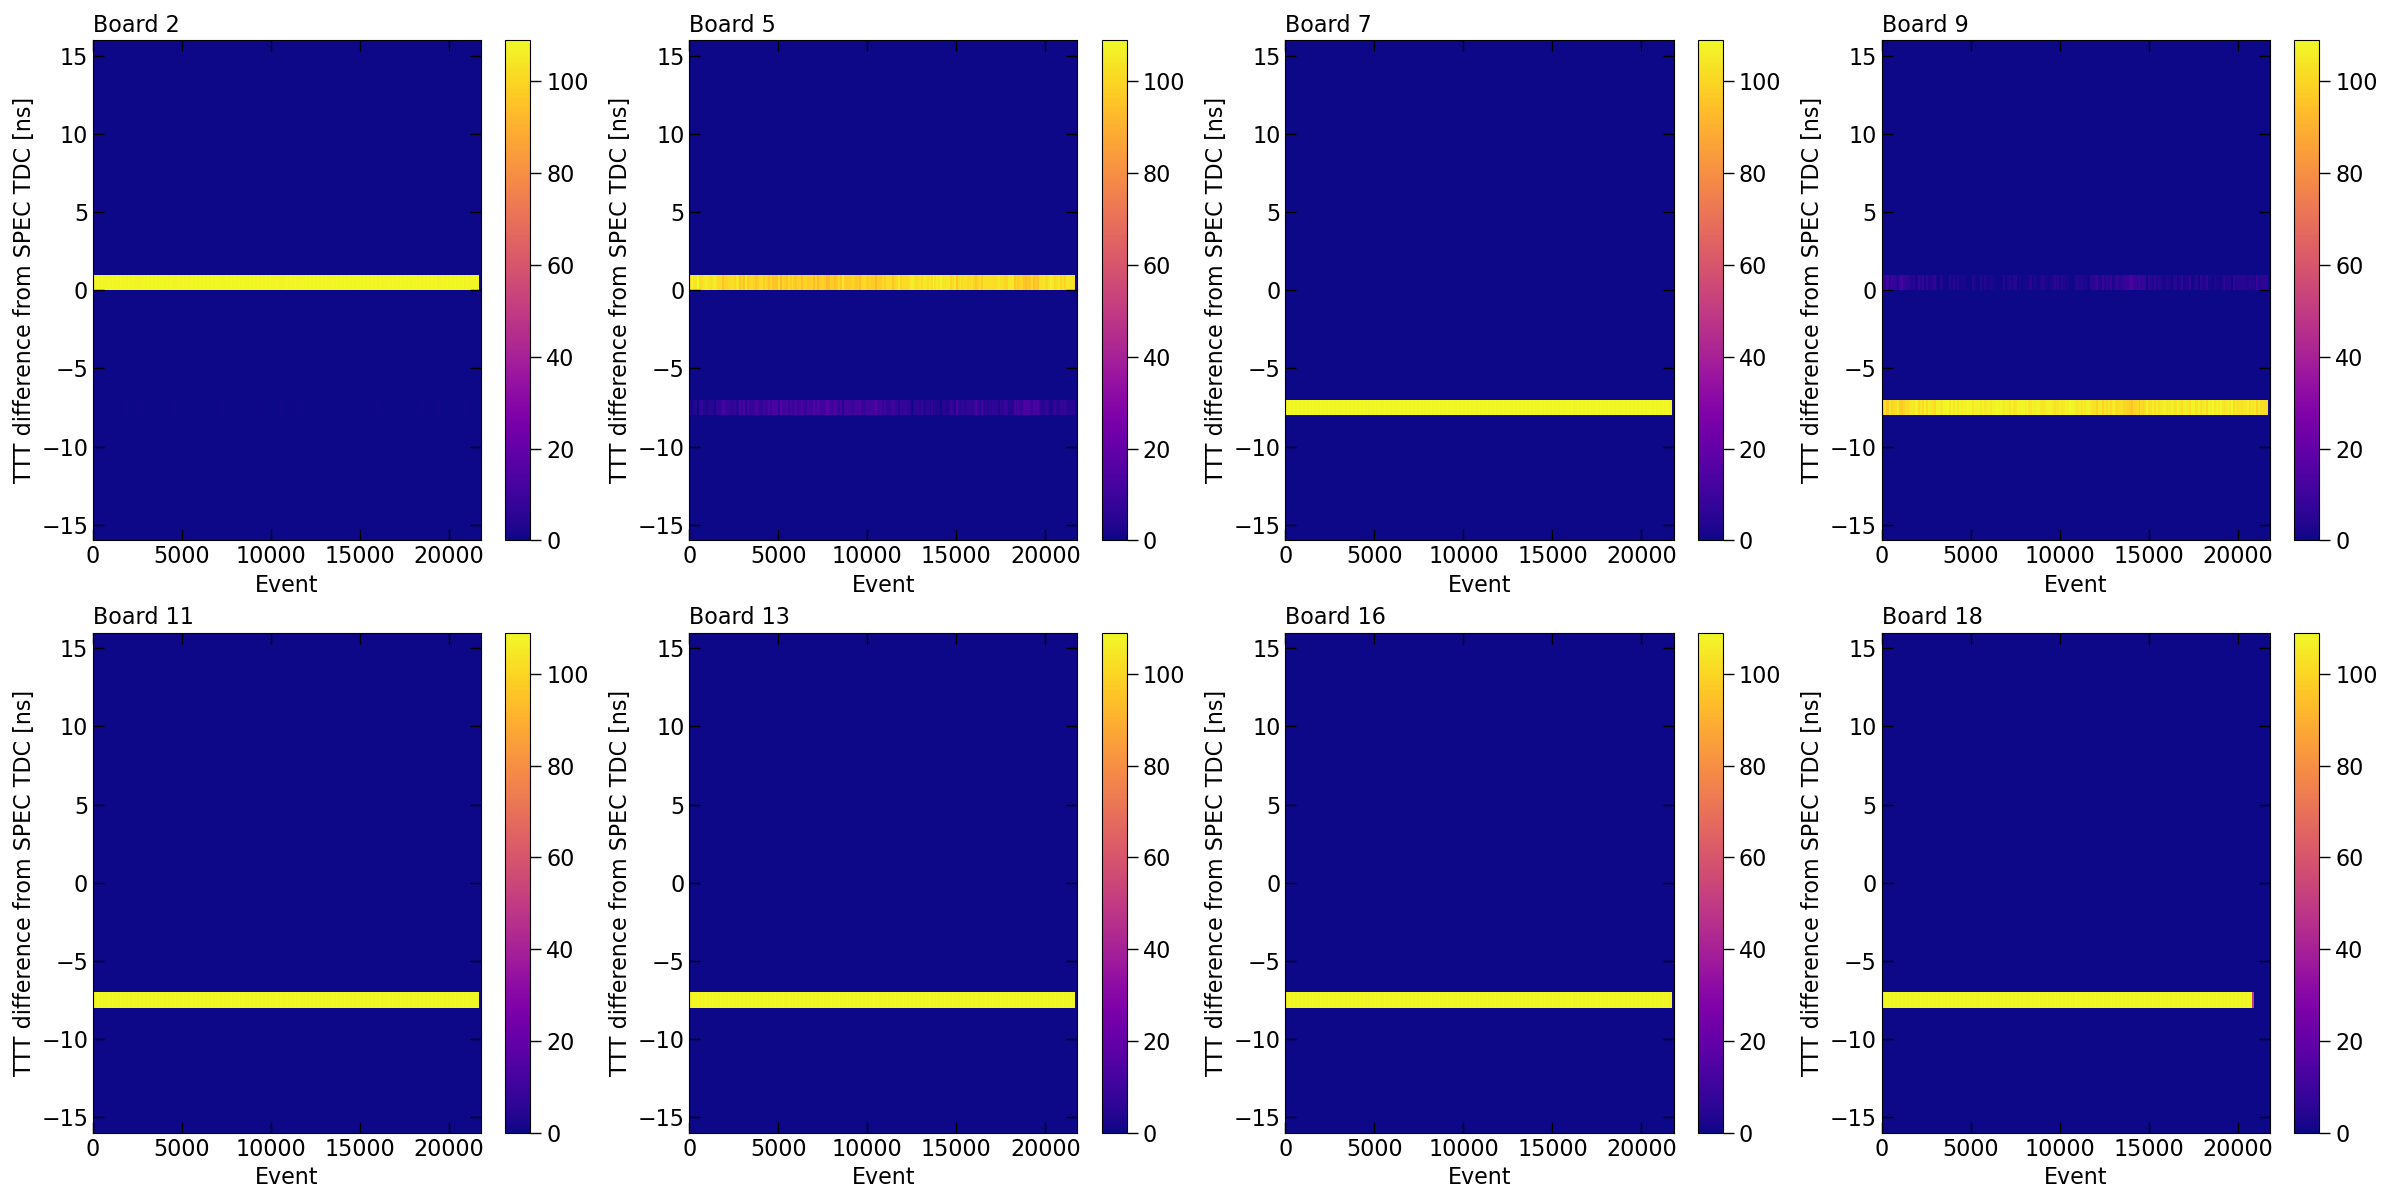
\includegraphics[width=\linewidth]{TTT_SPEC_diff_run8060}
\caption{Run 8060}
\end{subfigure}%
\caption[daisychainSPEC]{
The comparison of the timestamps produced by the CAEN digitizer against those produced by the SPEC-TDC with the CAEN digitizers employing the daisy chain clock scheme.
Run 7980 shows perfect synchronisation whilst run 8060 shows the effect of clock drifting in a daisy chain clock scheme.
}
\label{fig:daisychainSPEC}
\end{figure}

%Result from daisy chain
The daisy chain clock scheme underwent testing across multiple DAQ runs over a few days. 
An example of the results is shown in Fig. \ref{fig:daisychainSPEC} for run 7980 and run 8060.
The results for run 7980 demonstrates perfect synchronisation across all 8 CAEN digitizers, as well as synchronisation with respect to the SPEC-TDC, and thus the PPS signal.
All the timestamps agree within a single nanosecond and remain stable during the full run.
In contrast, run 8060 was taken 4 days after run 7980 and exhibited interesting effects.
Board 7 in the daisy chain drifted by 8 ns, causing all subsequent boards in the daisy chain to also drift, yet they remained synchronised with each other. 
Moreover, board 5 also shows a straddling effect, resulting in a jittering of 8 ns.
This straddling behaviour is expected since the trigger clock of CAEN digitizer is read every 2 clock cycles, introducing fluctuations twice the tick value of 8 ns.
Both these runs also show that board 18 stopped taking data a while into the DAQ run, which was found to be due to a malfunctioning temperature sensor in this CAEN digitizer.
This digitizer was sent away to the manufacturer for repair.

\begin{figure}[htbp!]
\begin{subfigure}[h]{1.00\linewidth}
\centering    
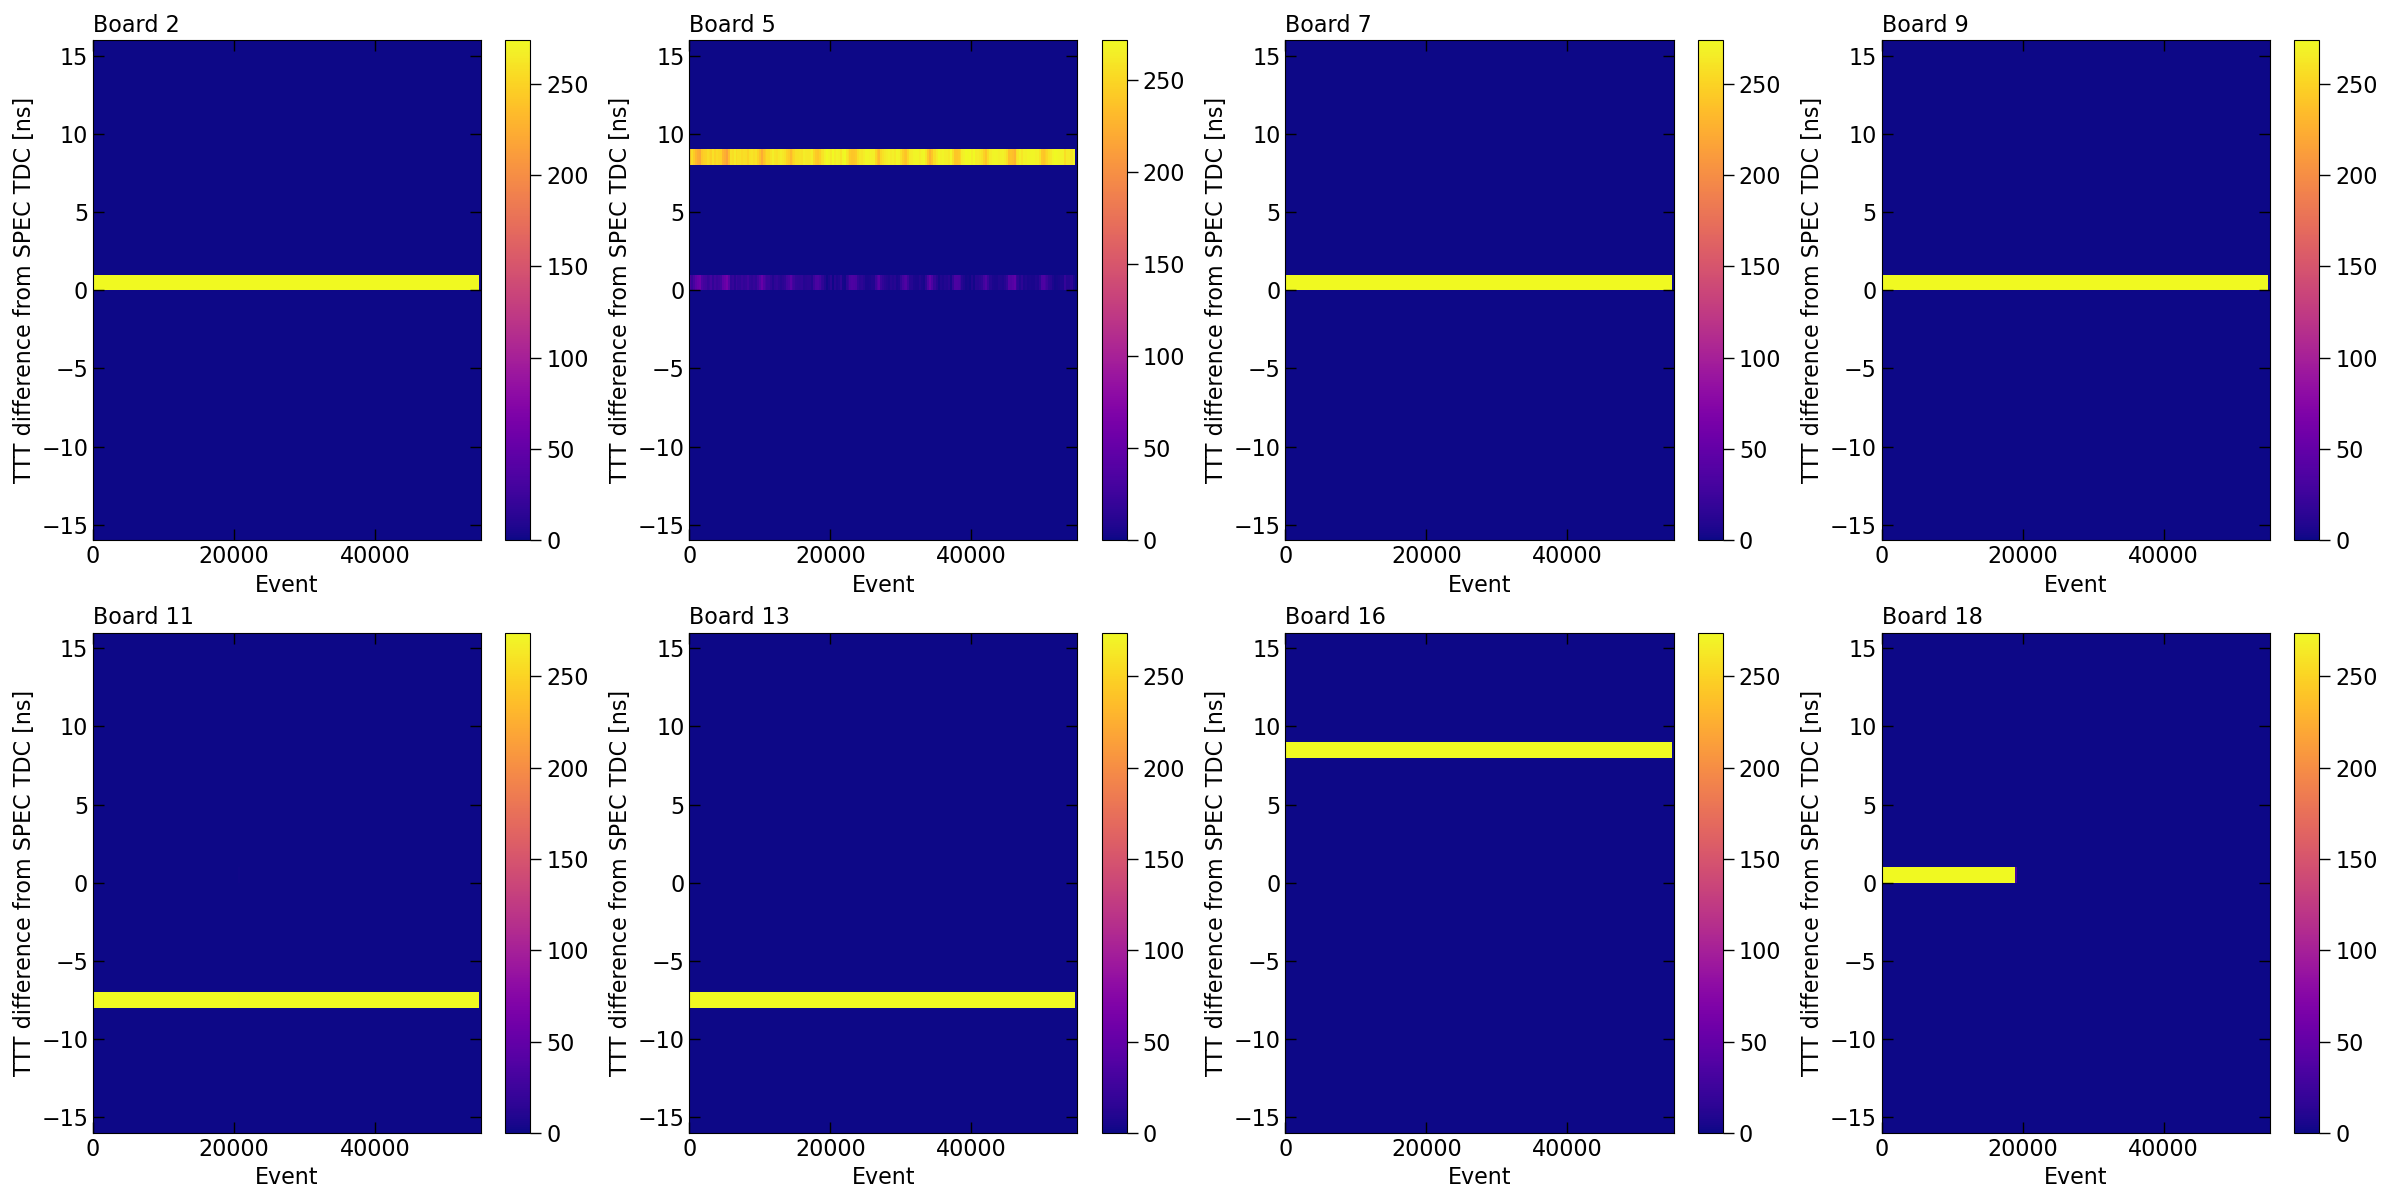
\includegraphics[width=\linewidth]{TTT_SPEC_diff_run8178}
\caption{Run8178}
\end{subfigure}
\hfill
\begin{subfigure}[h]{1.00\linewidth}
\centering    
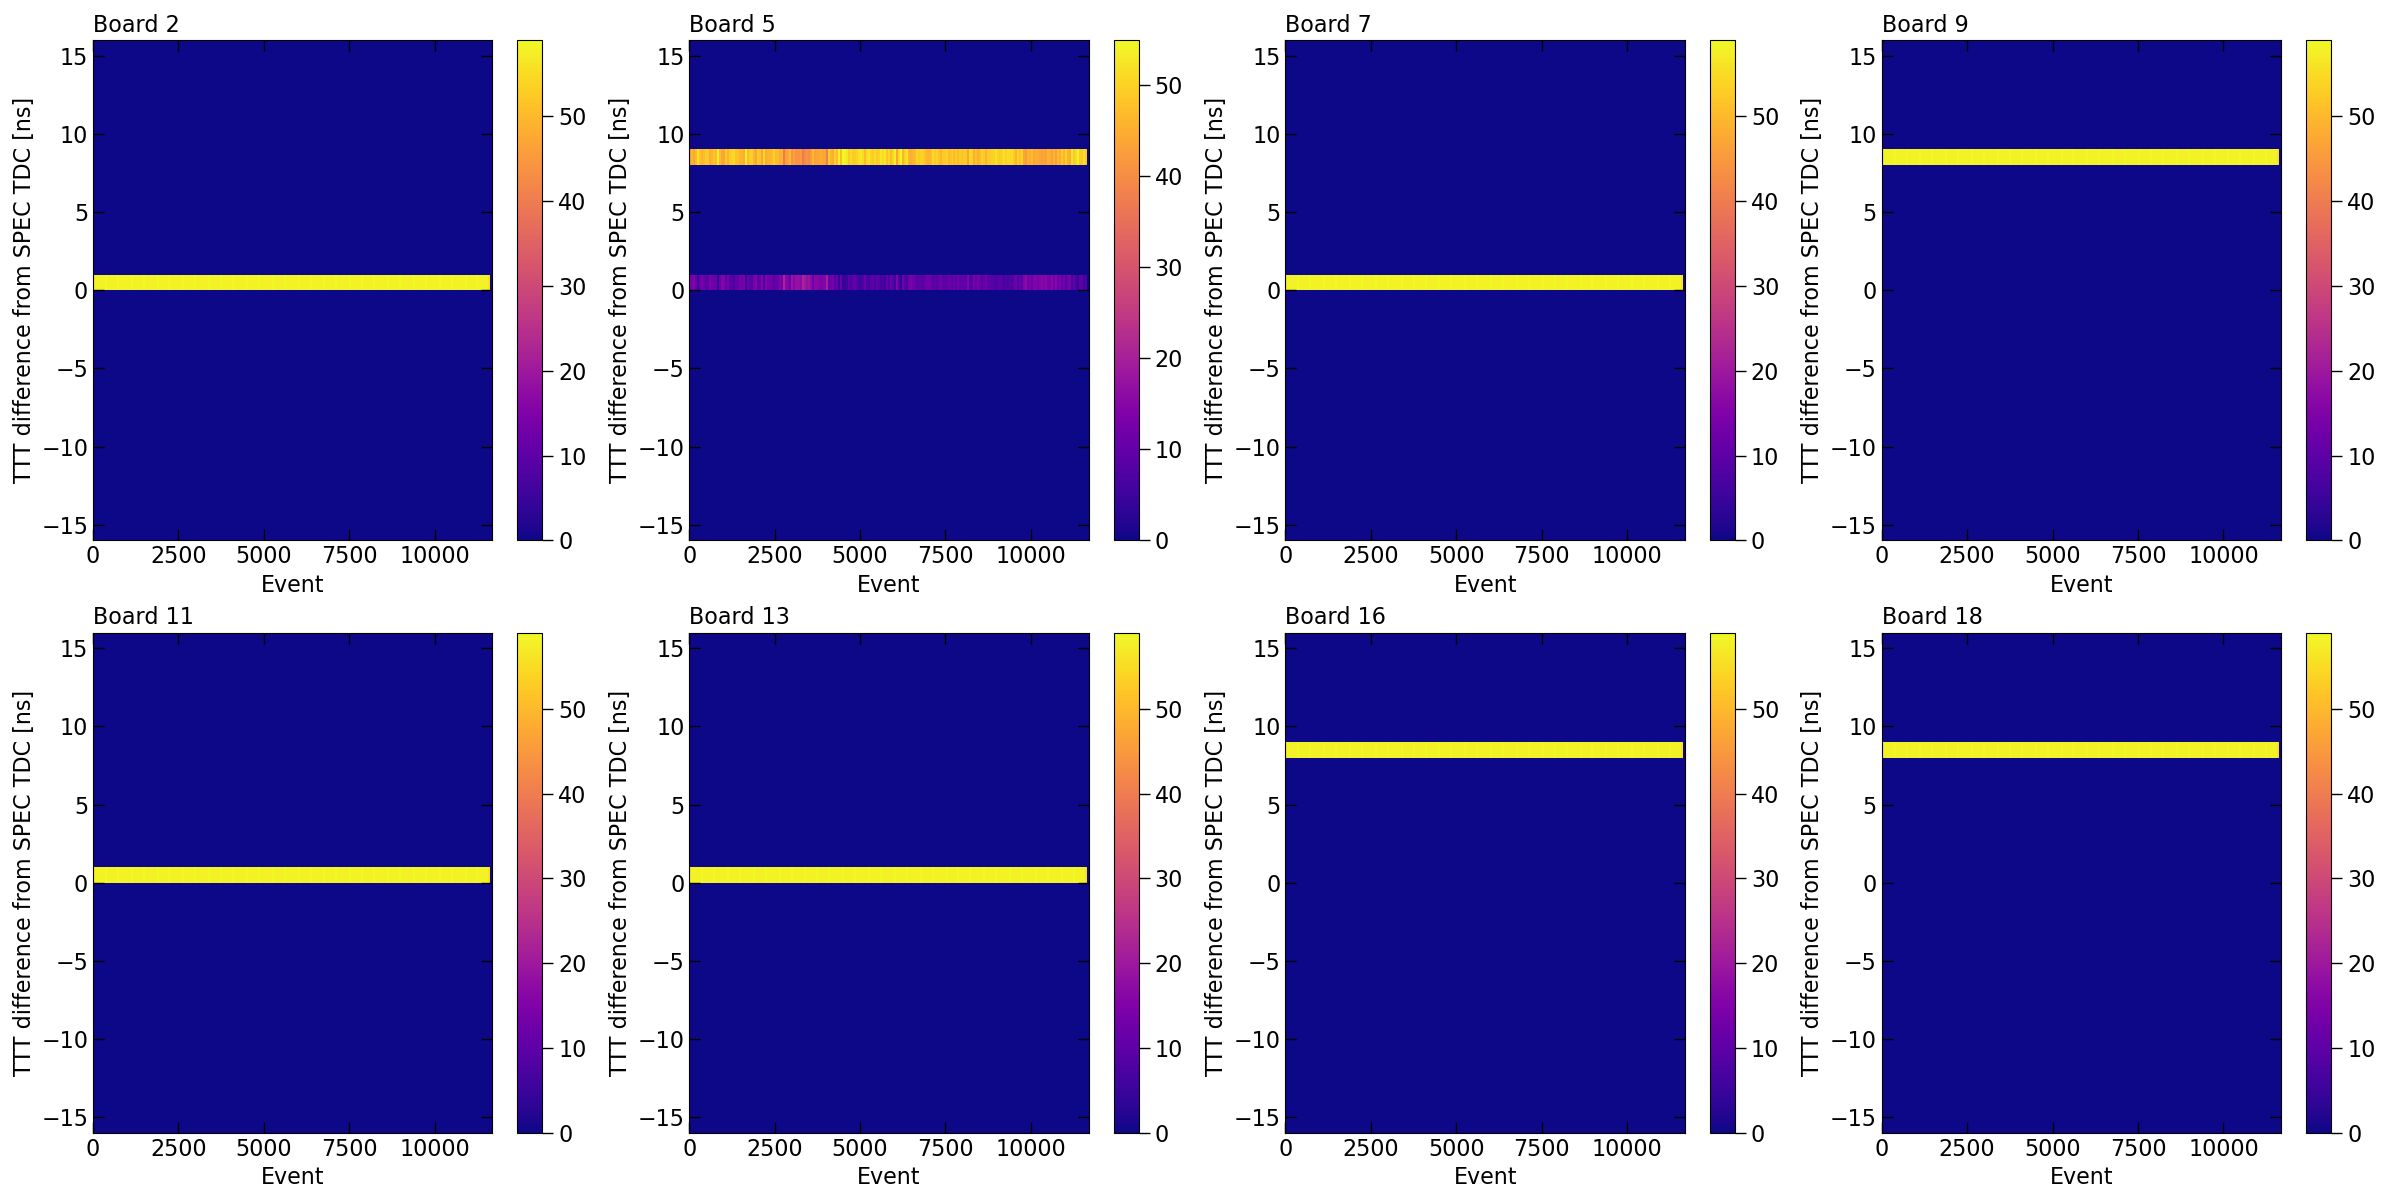
\includegraphics[width=\linewidth]{TTT_SPEC_diff_run8196}
\caption{Run 8196}
\end{subfigure}%
\caption[fanoutSPEC]{
The comparison of the timestamps produced by the CAEN digitizer against those produced by the SPEC-TDC with the CAEN digitizers employing the fan out clock scheme.
Since the input frequency of 10 MHz is not phase with the trigger clock frequency of 125 MHz, this introduces a random phase offset in timestamps across all the digitizers and different runs. 
}
\label{fig:fanoutSPEC}
\end{figure}

%Result from fan out
The same test was repeated for the fan out clock fan scheme, where multiple DAQ runs were conducted over a few days.
An example of the run results is shown in Fig. \ref{fig:fanoutSPEC} for run 8178 and run 8196.
In both of these runs, board 5 shows the same straddling effect, causing timestamps to jitter by 8 ns.
One key difference in this clock scheme is that the timestamps recorded by each CAEN digitizer varies randomly between digitizers and across different runs. 
This variation is due to the input frequency to the CLK-IN connector set at 10 MHz.
As previously explained, the trigger clock is generated by the AD9510 chip, which must be in phase with the input frequency. 
However, the trigger clock operates at a frequency of 125 MHz, while the input frequency remains at 10 MHz. 
Since these frequency values are not multiples of each other, they do not agree in phase.
To generate an out-of-phase frequency, the AD9510 chip latches onto the first rising edge of the input frequency upon the digitizer initialisation. 
Consequently, when the CAEN digitizer is initialised at the beginning of every DAQ, a random phase offset is introduced, causing the timestamps to vary from run to run.
Moreover, the 10 MHz clock is distributed in fan out scheme to every digitizer resulting in the phase offset varies randomly from one digitizer to another.

%settle for daisy chain over fan
Comparing between the two clock schemes, the daisy chain mode offers better synchronisation across the 8 CAEN digitizers compared to the fan out mode.
In the daisy chain scheme, only the first CAEN in the daisy chain receives the external 10 MHz clock.
The master clock CAEN digitizer can have a random phase offset that propagtes down the daisy chain, resulting in synchronisation across all digitizers.
However, it is important to note that the clock drift effect has been observed while testing the daisy chain scheme
Monitoring these effects during the commissioning period is necessary to understand the impacts of the clock drift."

\subsection{Clock Jittering Correction}

To further characterise the timing resolution of the CAEN digitizer, an additional test was added to understand how precisely the board digitizes the waveform.
As demonstrate in Fig. \ref{fig:TTTDiagram}, the TTT object is the timestamp of the last tick of waveform, and thus, this provides the timing information to construct the timing of the waveform.
From the manuals of the digitizer, it is indicated that the trigger clock and the ADC sampling clock are synchronised with respect to each other.
Thus, this test aimed to test whether all 8 CAEN digitizers can digitize waveform in synchronisation with each other within a nanosecond. 

\begin{figure}[htbp!] 
\centering    
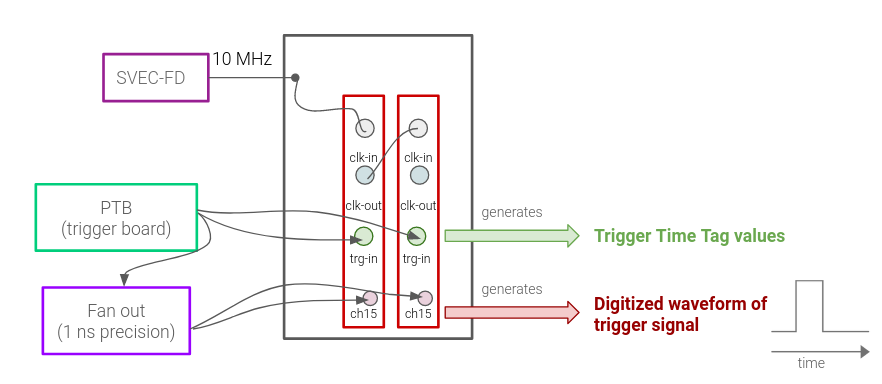
\includegraphics[width=1.0\textwidth]{digitize_ftrig}
\caption[digitizeFTRIG]{
The set up for study the synchronisation of the CAEN digitizers and their timing resolution.
In this set up, the 1 Hz trigger is produced from the PTB, and input into the TRG-IN channel of each CAEN for simultaneous triggering.
The timestamp of the trigger is embedded in the Trigger Time Tag object.
The trigger is also propagate to a fan out module, and input into channel 15 of every CAEN digitizer.
The waveform of the trigger signals is expected to be digitized simultaneously. 
}
\label{fig:digitizeFTRIG}
\end{figure}

%setup
This study used the same set up as described in the previous section.
An additional setup was to input the trigger into channel 15 of every CAEN digitizer with the same amount of cable length so that all triggers would be digitized simultaneously as shown in Fig. \ref{fig:digitizeFTRIG}.
In this configuration, the trigger would be timestamped in the TTT object, as well digitized as a waveform. 

%two different modes to compare timestamp
This set up presents two types of timestamps produced by the CAEN digitizer.
As illustrated in Fig. \ref {fig:TTTDiagram}, one timestamp is derived from the TTT value produced by the trigger clock of the CAEN digitizer.
These timestamps were examined in the synchronisation study in section \ref{subsec42PMT}.
This type of timestamp is now referred as the TTT-derived timestamp.
Given that the waveform of the trigger signal is now digitized, one can determine the rising edge of the trigger signal.
This gives a tick value on the waveform and thus, the timestamp associated to this tick which can be derived from the TTT value.
This type of timestamp is referred as the tick-derived timestamp, since this timestamp requires the knowledge of the tick position of the trigger on the waveform as well as the TTT value.
Both these timestamps are compared against the SPEC-TDC timestamps of the trigger signals, to the same reference frame at which the trigger leaves the PTB front face.
Cable length corrections were also applied.

\begin{figure}[htbp!] 
\centering    
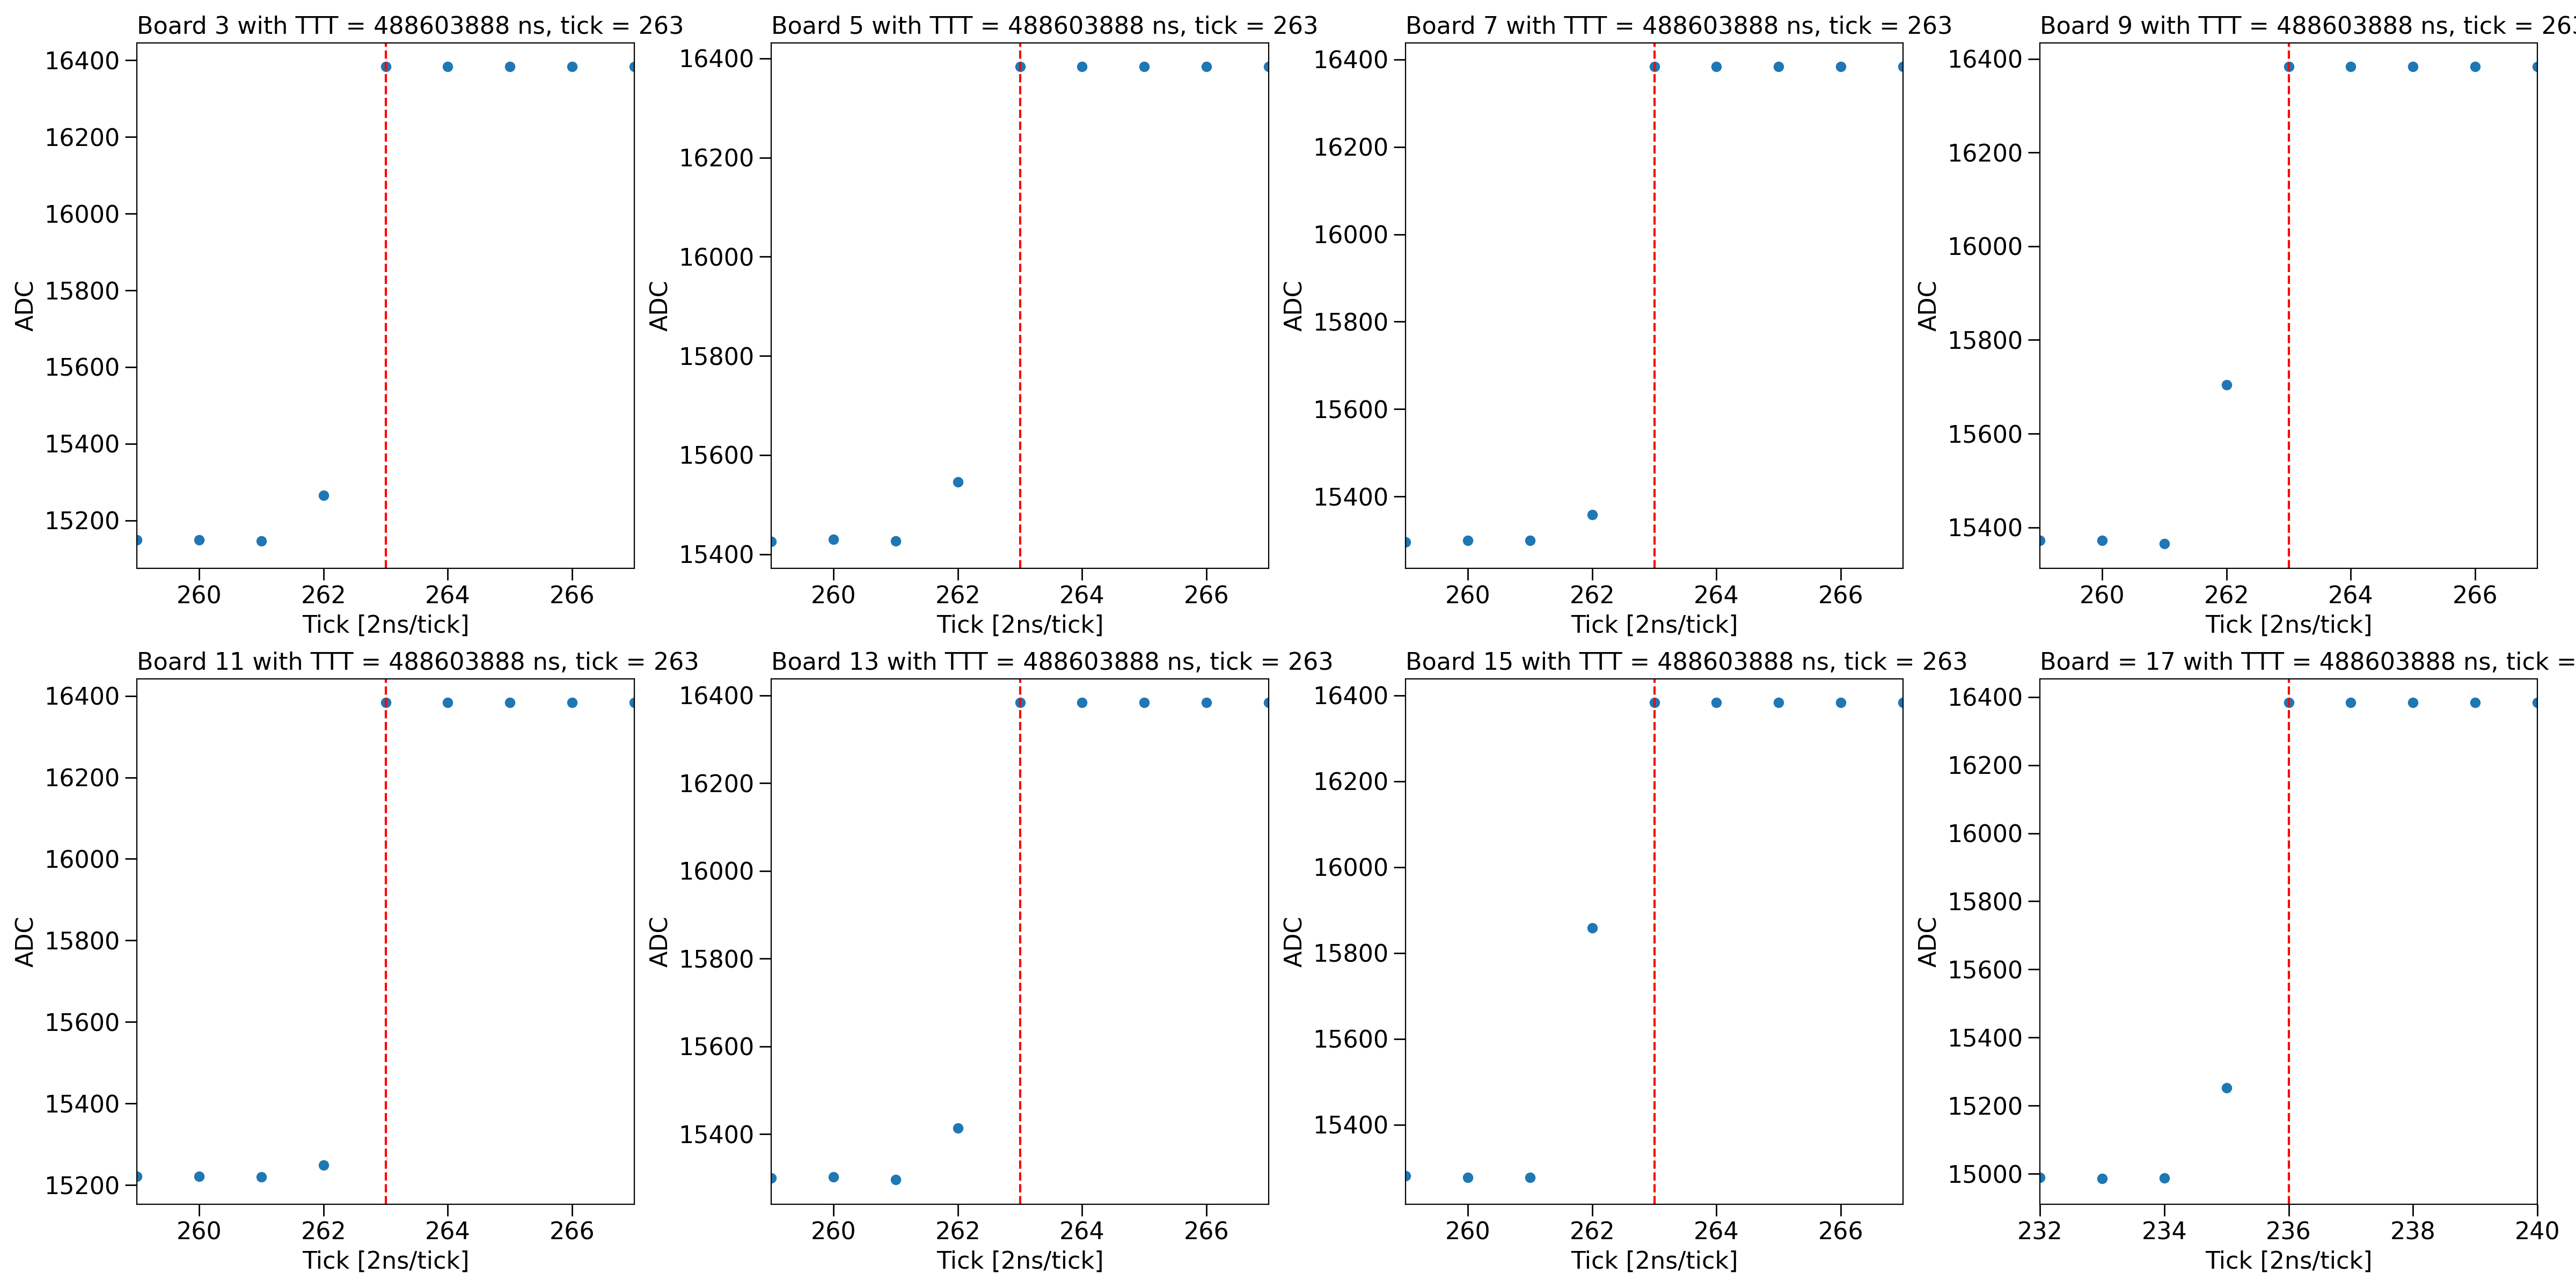
\includegraphics[width=1.0\textwidth]{daisychain_calib}
\caption[daisychainCALIB]{
After the daisy chain calibration, the waveforms of the simultaneous triggers are plotted to check for synchronisation.
The TTT values associated with the each waveform are identical, showing that the digitizers receive triggers at the same time.
The waveforms of the triggers are zoomed around the rising edge, showing the identical tick value of the rising edge, showing that all the boards also digitize the trigger at the same time.
Board 17 is an exception because it has a different firmware compared to the rest of the digitizers and digitizes the waveform slightly different.
}
\label{fig:daisychainCALIB}
\end{figure}

The daisy chain clock scheme was also re-calibrated before conducting this study.
As described in section \ref{subsec41PMT} on the overview of the CAEN digitizer clock, the clock propagation from the master clock to the slave clock needs to be delayed with a precise amount such that their clocks are exactly in phase.
This calibration process was to ensure that not only every digitizer would produce identical timestamps for simultaneous triggers, but also would digitize the trigger signals simultaneously.
The result after the process is demonstrated in Fig. \ref{fig:daisychainCALIB}, showing that every digitizer has the same timestamp and digitizes the trigger signal at the exact same tick position on the waveform.As a result, the timestamps of the tick value on the rising edge of trigger signals, or the tick-rived timestamps, are identical across all 8 CAEN digitizers.

Multiple DAQ runs were taken for this study over a period of one month.
Each run duration varied from less than an hour up to 10 hours.
The purpose of this was also to test the stability of the synchronisation of the daisy chain and its impact on the resolution of the produced timestamps.
This timing resolution study was conducted on a dataset of 30 runs.

\begin{figure}[htbp!]

\begin{subfigure}[h]{1.00\linewidth}
\centering    
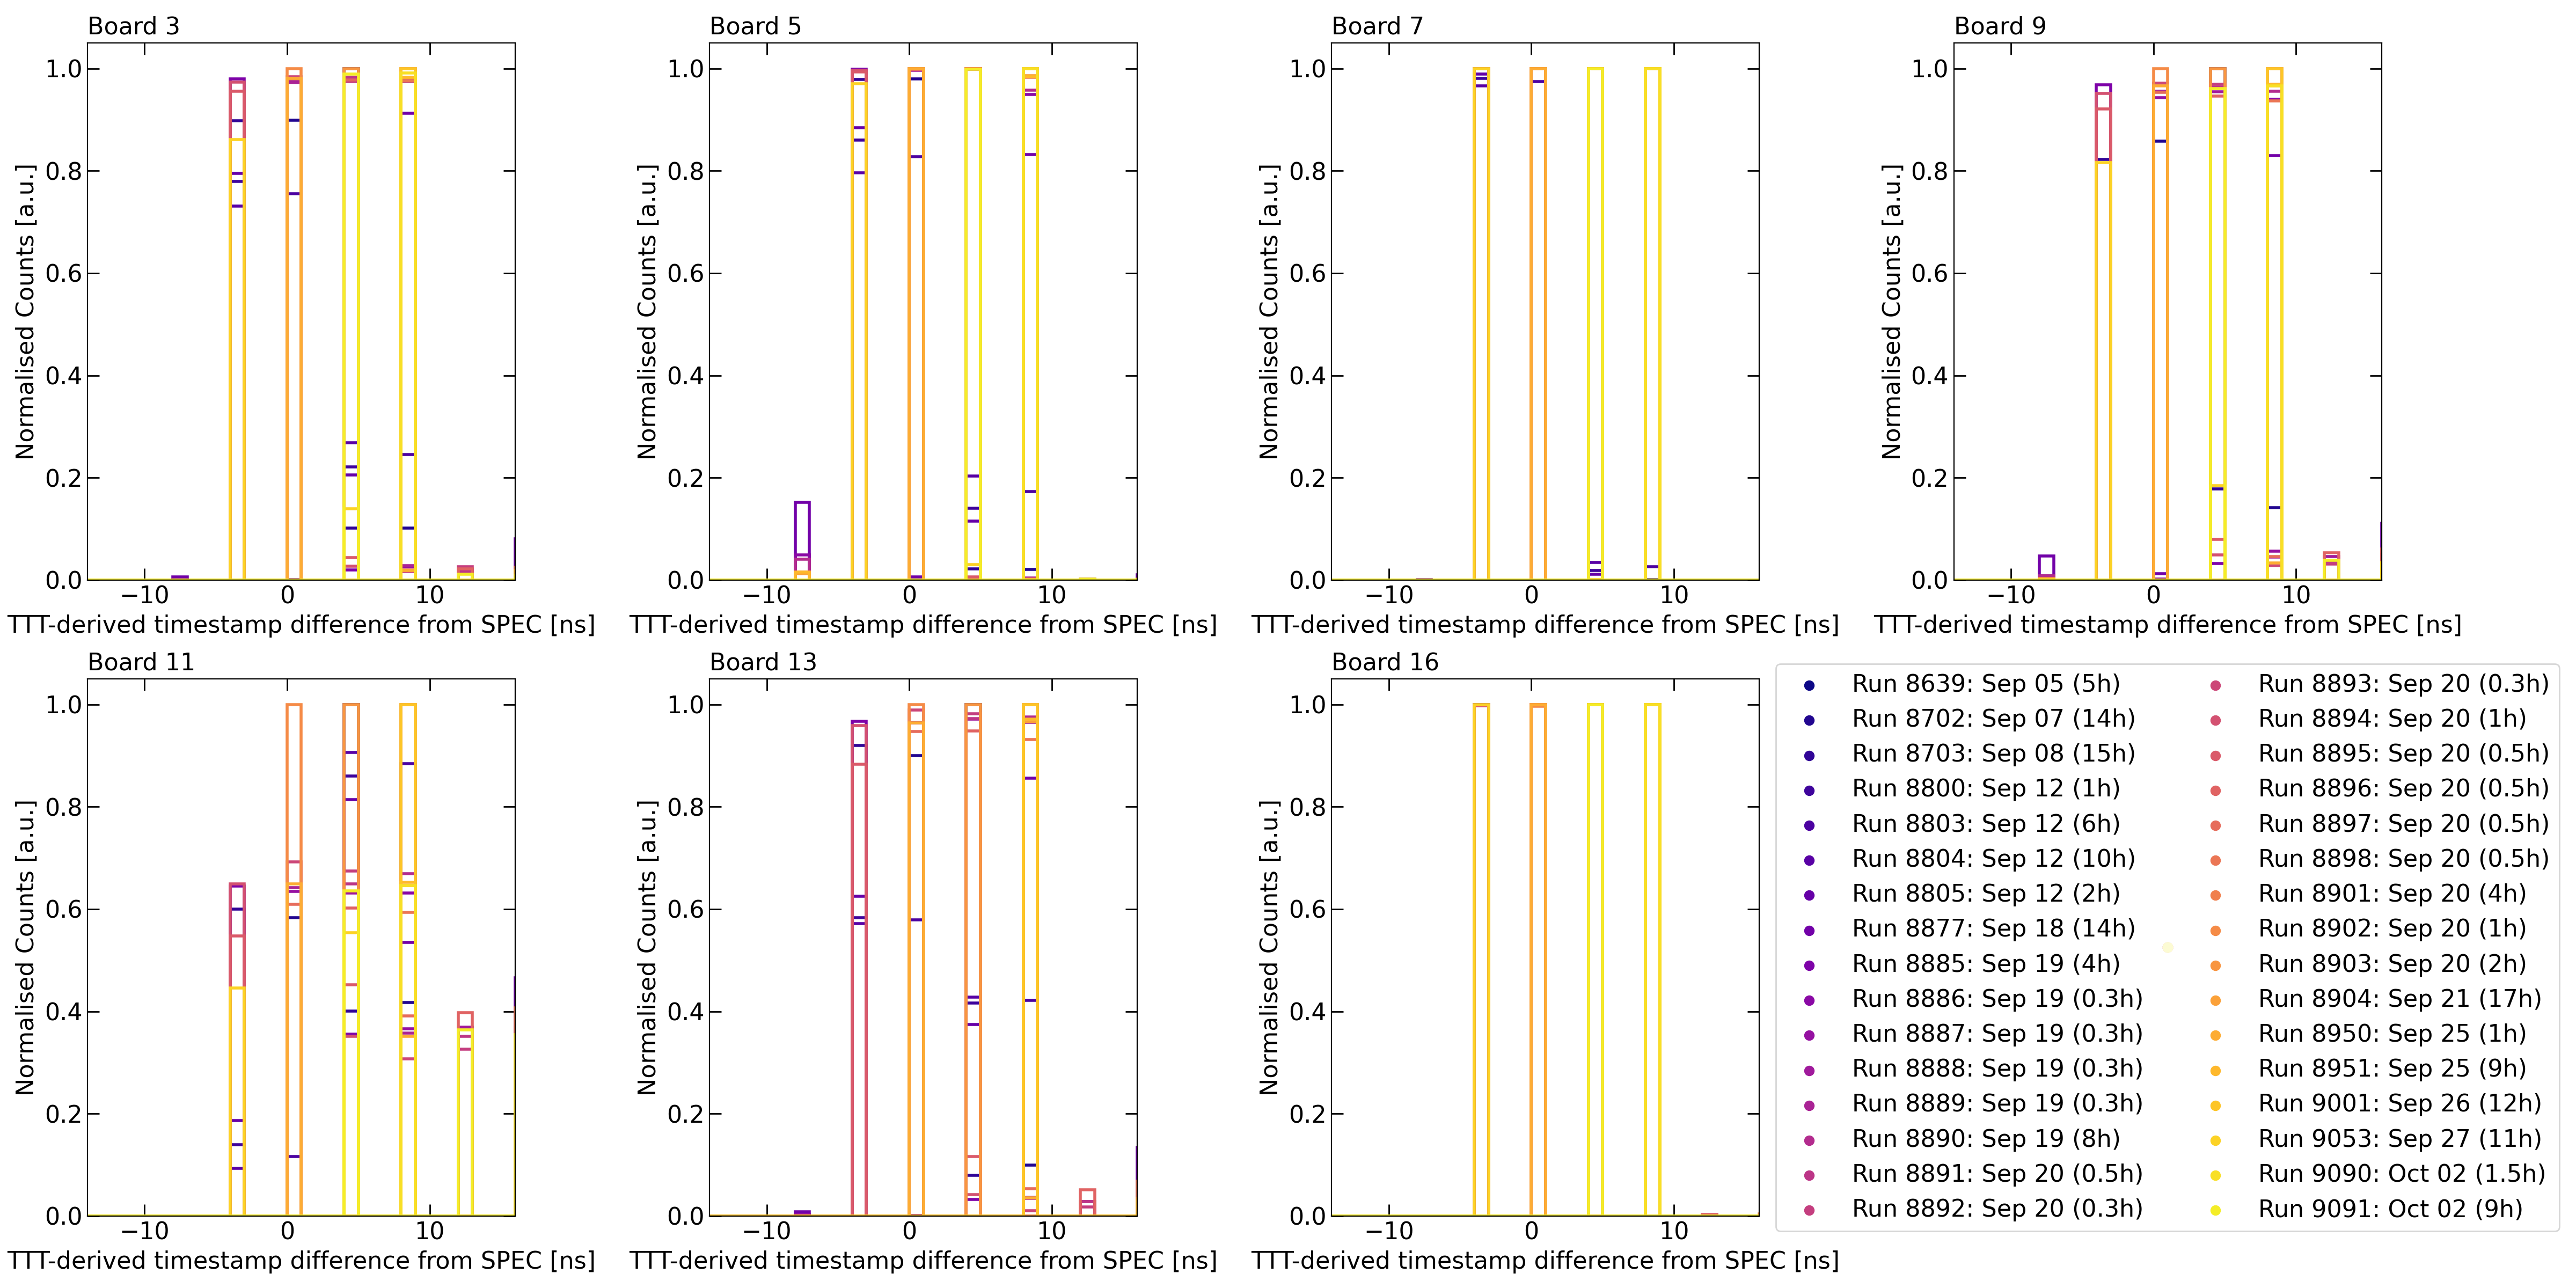
\includegraphics[width=\linewidth]{TTTts_spec}
\caption{TTT-derived timestamps}
\label{subfig:TTTts_spec}
\end{subfigure}

\hfill
\begin{subfigure}[h]{1.00\linewidth}
\centering    
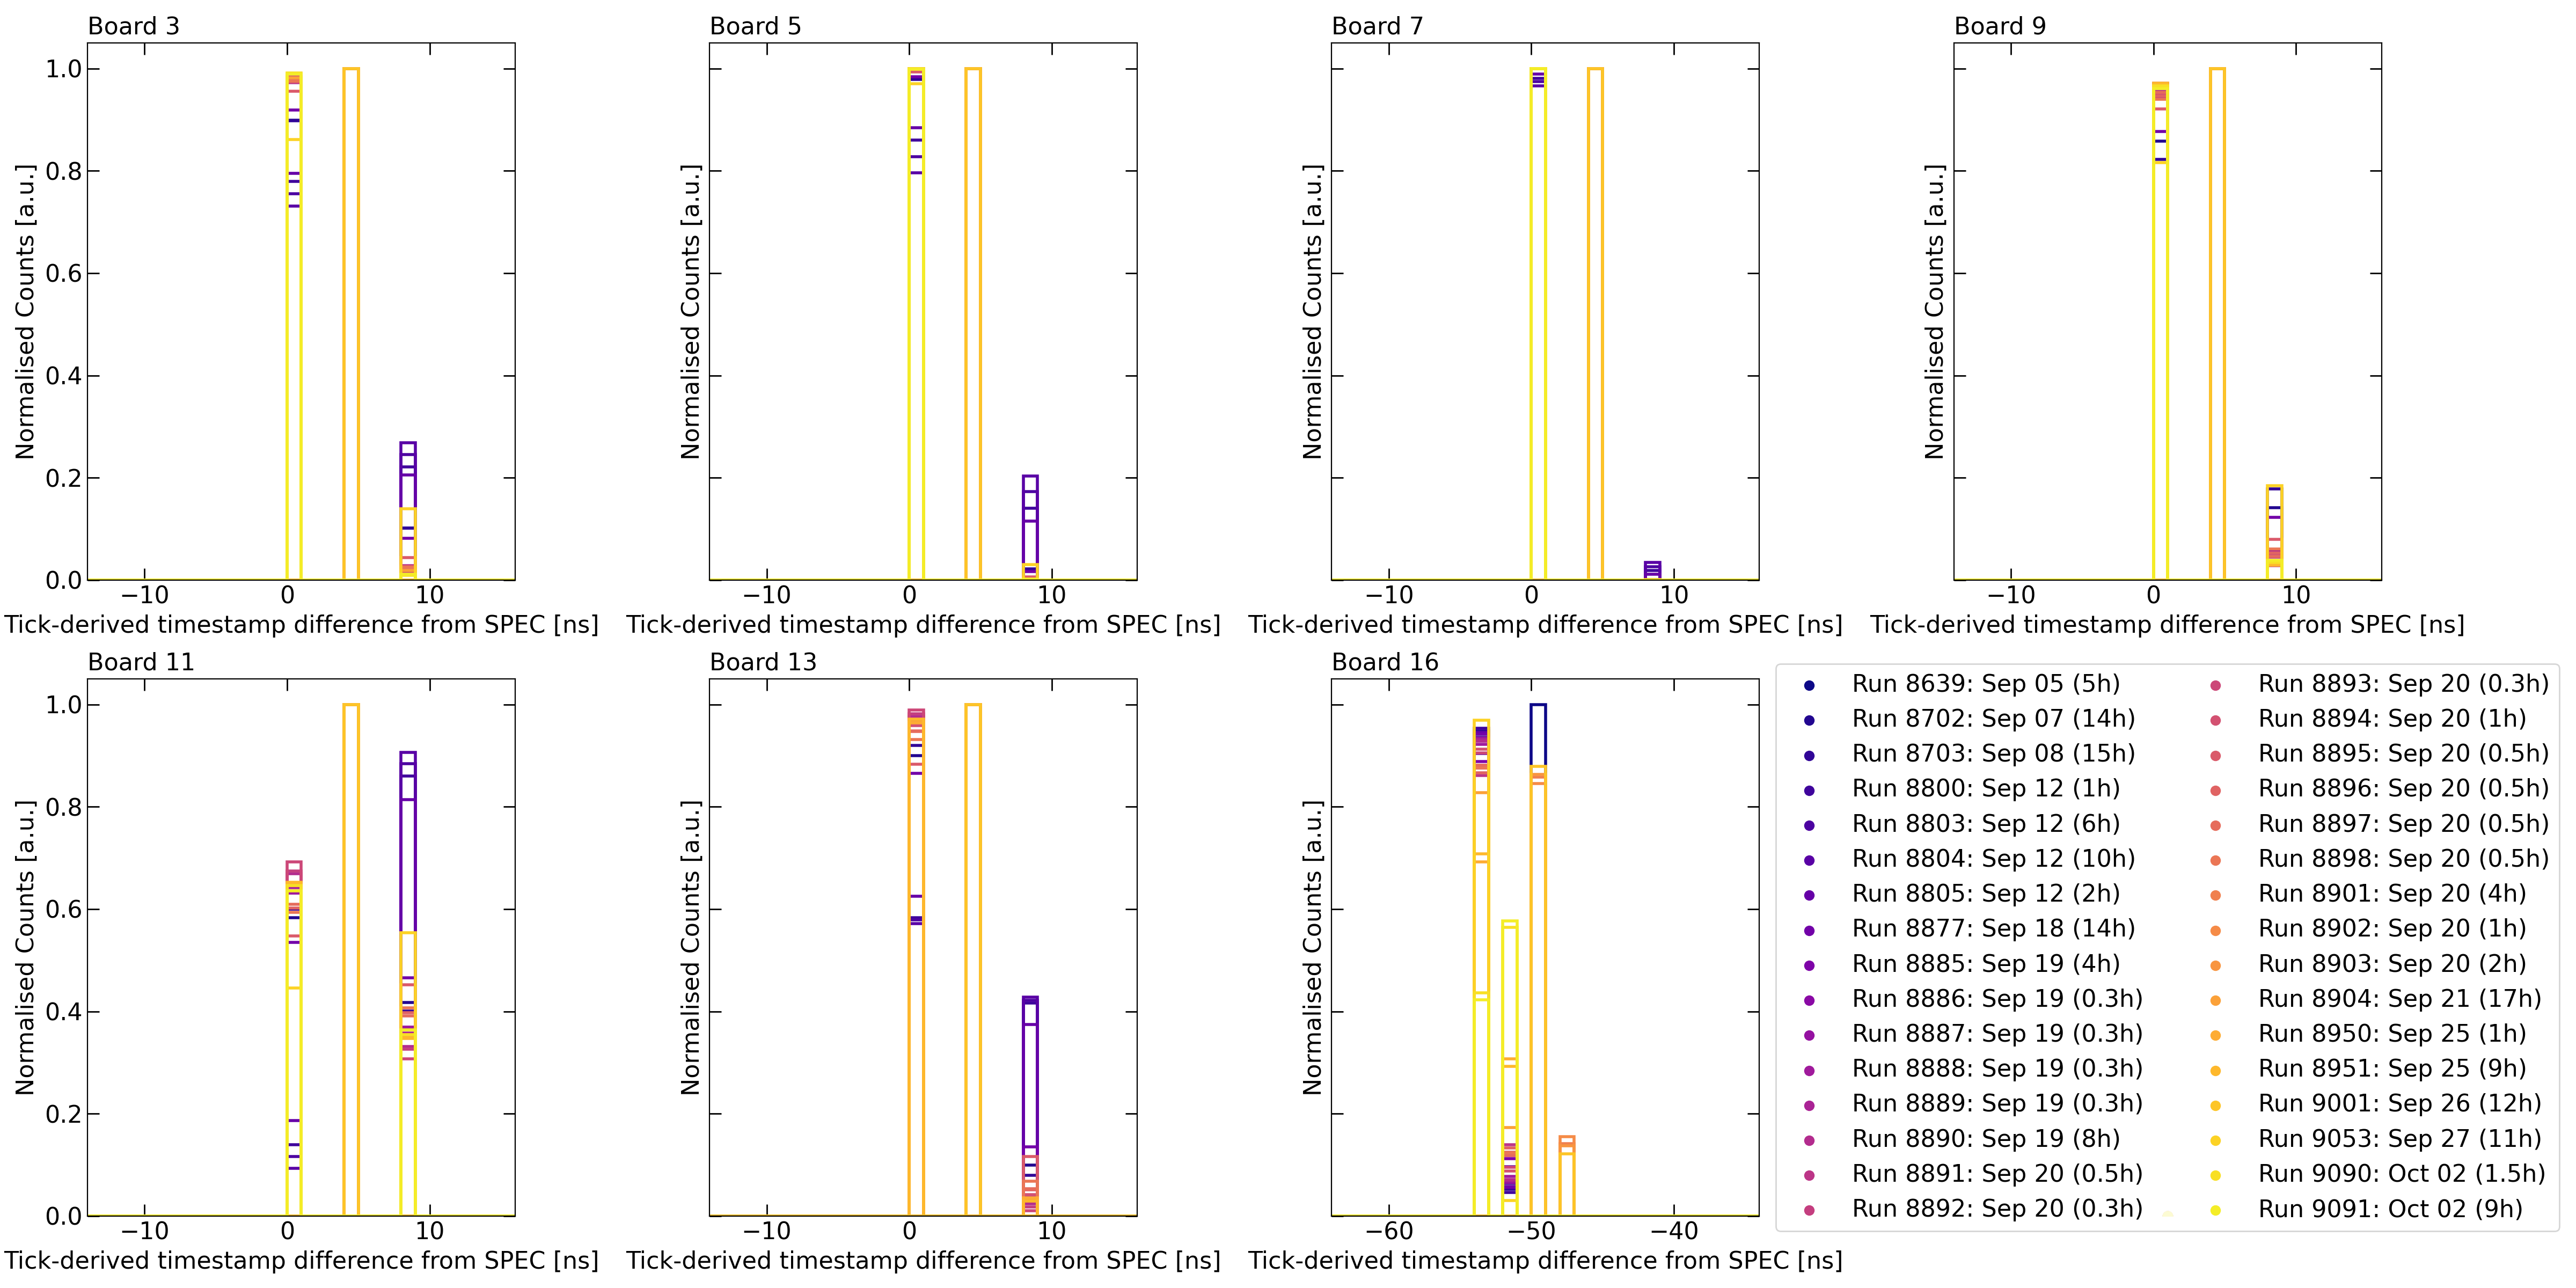
\includegraphics[width=\linewidth]{Tickts_spec}
\caption{Tick-derived timestamps}
\label{subfig:Tickts_spec}
\end{subfigure}%

\caption[TTTtsTickts]{
The two timestamps distributions generated by the CAEN digitizers, compared against the SPEC-TDC timestamps.
The TTT-derived timestamps show a large spread up to 24 ns whilst the Tick-derived timestamps show a much smaller spread of only 8 ns.
}
\end{figure}

%TTT timestamps
The TTT-derived timestamps distribution is plotted in Fig. \ref {subfig:TTTts_spec} for 7 CAEN digitizers, compared against the SPEC-TDC timestamps.
This distribution shows a large spread up to 24 ns, which indicates that TTT-derived timestamp has a variation larger than what is stated in the manuals, that the trigger clock resolution is 16 ns.
The tick-derived timestamps distribution is plotted in Fig. \ref {subfig:Tickts_spec}.
This distribution, however, shows a much small spread of only 8 ns.

To understand the differences between the two types of timestamps, the tick position of the rising edge of the trigger waveform is also plotted in Fig. \ref {fig:TickSPEC}.
The distribution shows a large spread up to 5 ticks, equivalent to 10 ns.
This illustrates that the CAEN digitizer does not consistently digitize the trigger waveform, causing variations in the tick position of the rising edge between different events, run and digitizers.
This implies that not only can the trigger clock of the CAEN digitizer jitter, but its ADC sampling clock can also fluctuate, potentially introducing additional smearing.

\begin{figure}[htbp!]
\centering    
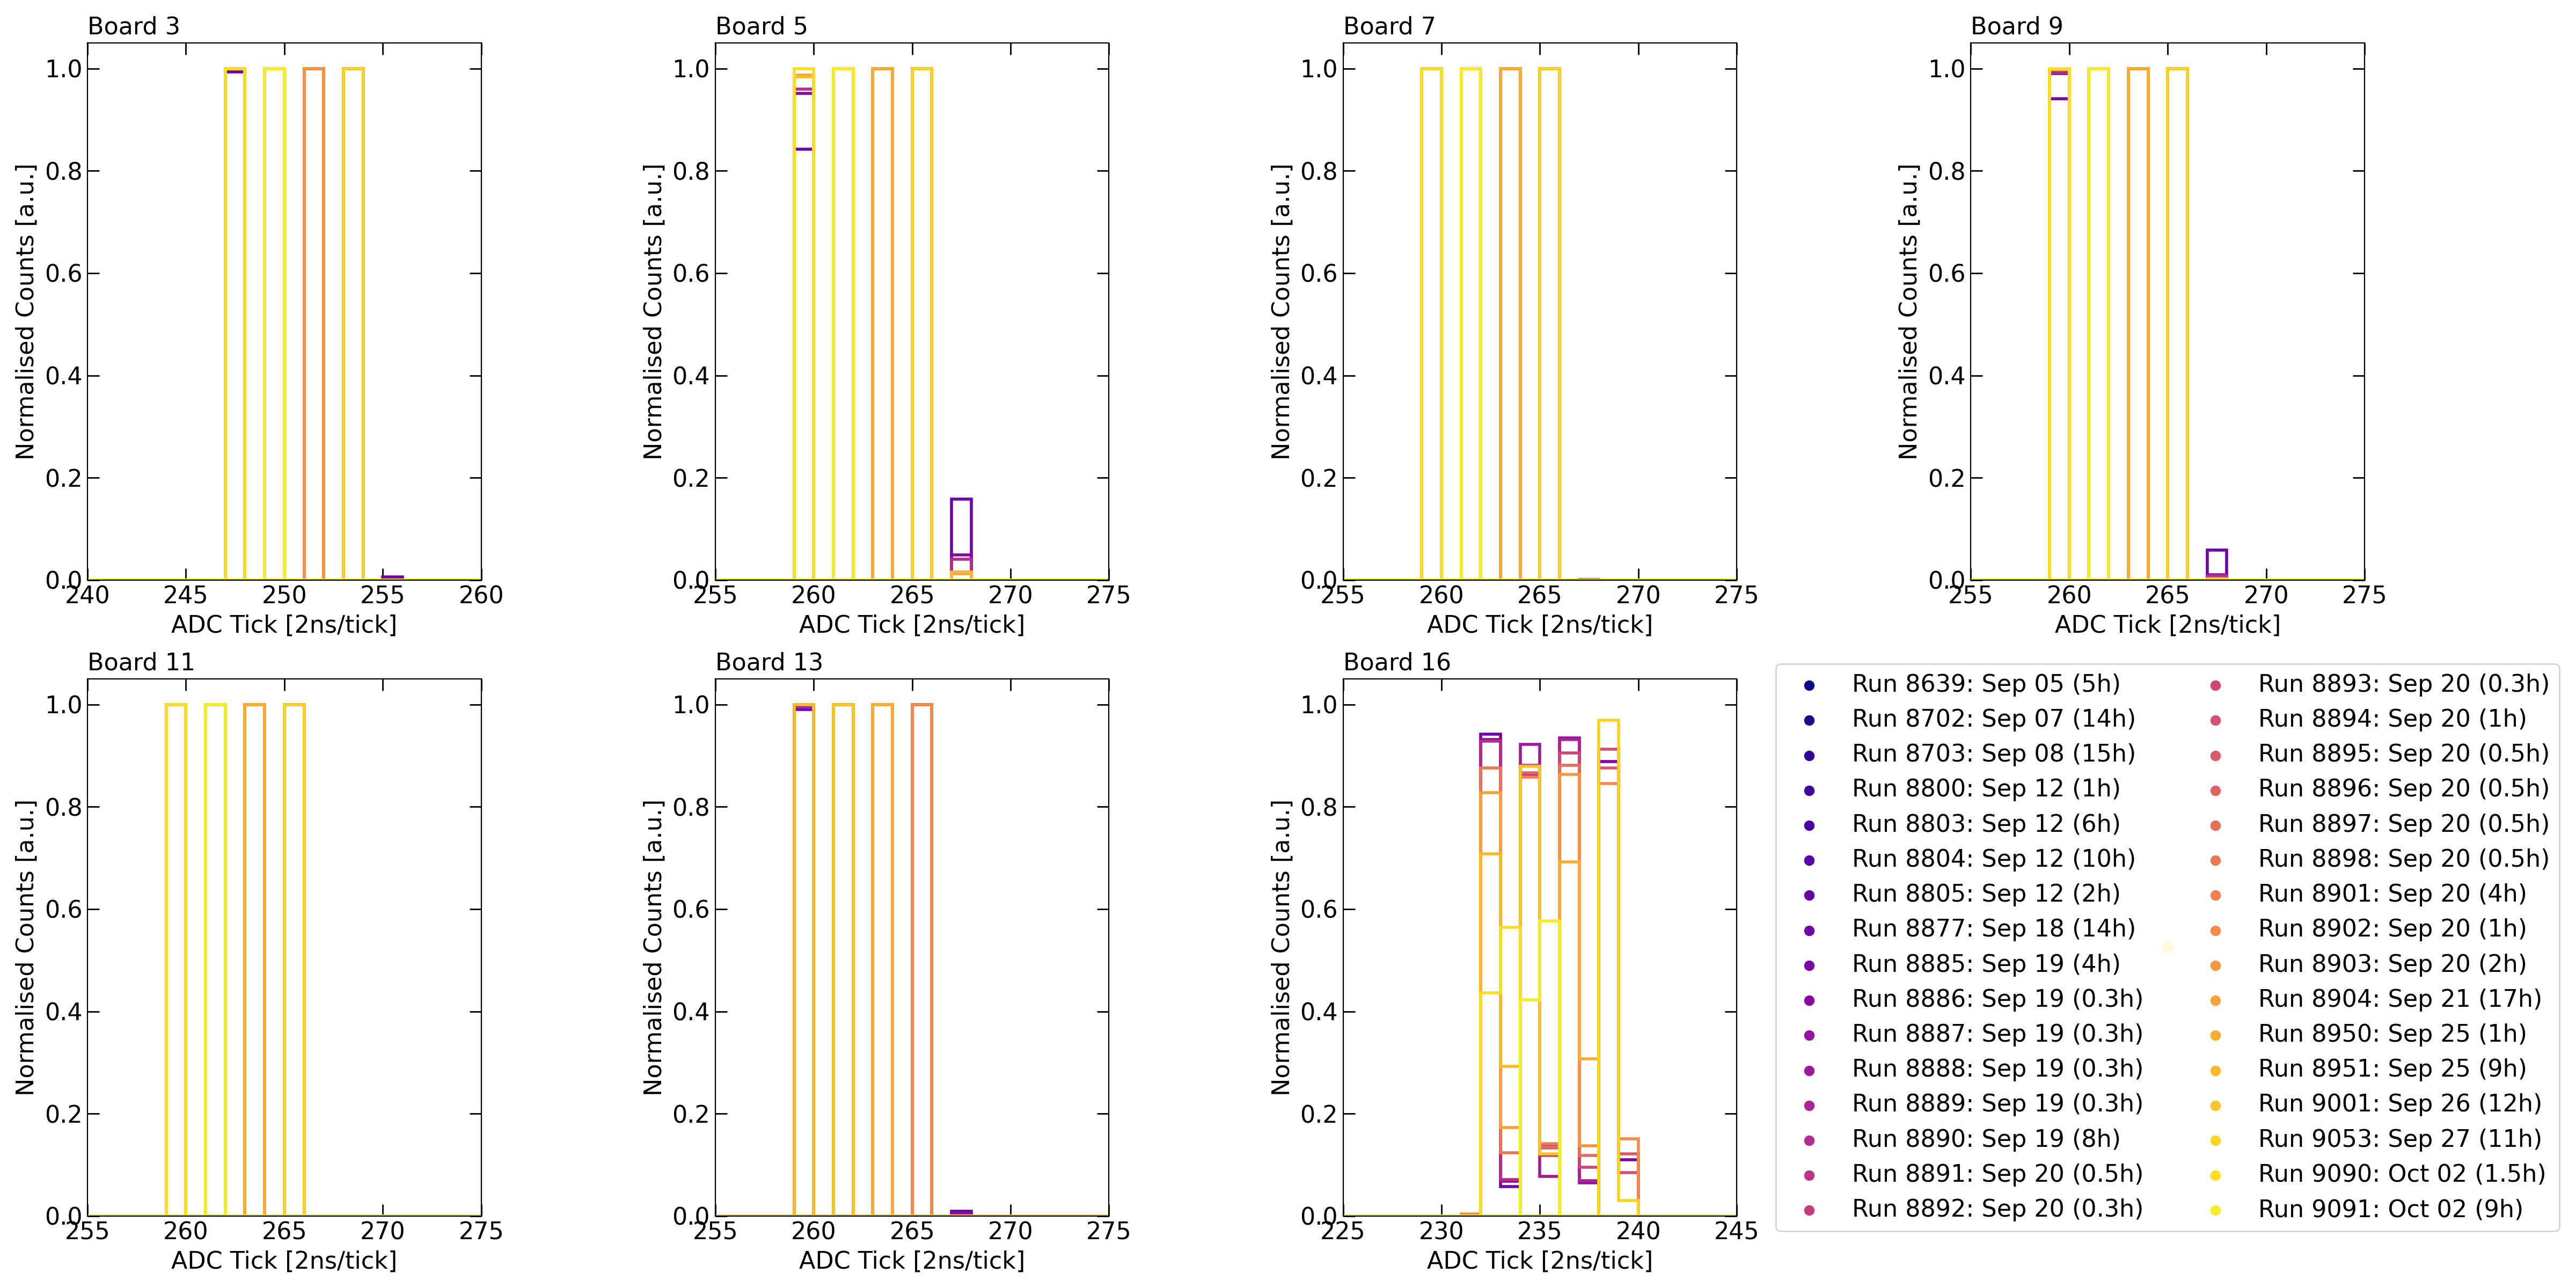
\includegraphics[width=\linewidth]{Tick_spec}
\caption[TickSPEC]{
The distribution of the tick value of the rising edge of the trigger waveforms has variation up to 5 ticks, equivalent to 10 ns. 
This demonstrates that the ADC sampling clock of the CAEN digitizer can also jitter.
}
\label{fig:TickSPEC}
\end{figure}

The CAEN manuals highlight that the trigger clock and the ADC sampling clock are correlated to each other, and this is reflected in the fact that the TTT value points to the last tick of the wave form.
The CAEN digitizer was designed on purpose to have the trigger clock in synchronised with the ADC sampling clock, so that the trigger clock can track and absorb the jittering of the ADC sampling clock.
This explains the 24 ns spread of the TTT-derived timestamps since it contains the smearing from both the trigger and the ADC sampling clocks.
Meanwhile, the tick-derived timestamps distribution shows a much smaller spread of 8 ns, since tht timestamp was produced using both the TTT value and tick value, resulting in a high level of precision.

%jittering cases
This understanding of the clock behaviour of the CAEN digitizer opens up venues for correcting for the timestamp jittering.
The tick-derived timestamp dataset were further examined in order to understand how to apply the correction to completely remove the 8 ns spread.
Three cases of jittering were identified and illustrated in Fig. \ref{subfig:jitter_before},  
The first case occurs when the ADC sample can jitter whilst the triggering clock remains stable.
This results in a different tick value of the rising edge, and introduces a tick-derived timestamp is smeared out by the ADC sampling clock tick value of 2 ns.
In the second case, the opposite situation arises such that the tick value of the rising edge is stable however the trigger clock jitters in step of 8 ns, resulting in the smearing of tick-derived timestamp by the same amount.
The last case is the combination jittering from both clocks, such that the smearing amount is a sum of the trigger and ADC sampling clock tick value, equal to 10 ns.

\begin{figure}[htbp!]

\begin{subfigure}[h]{1.00\linewidth}
\centering    
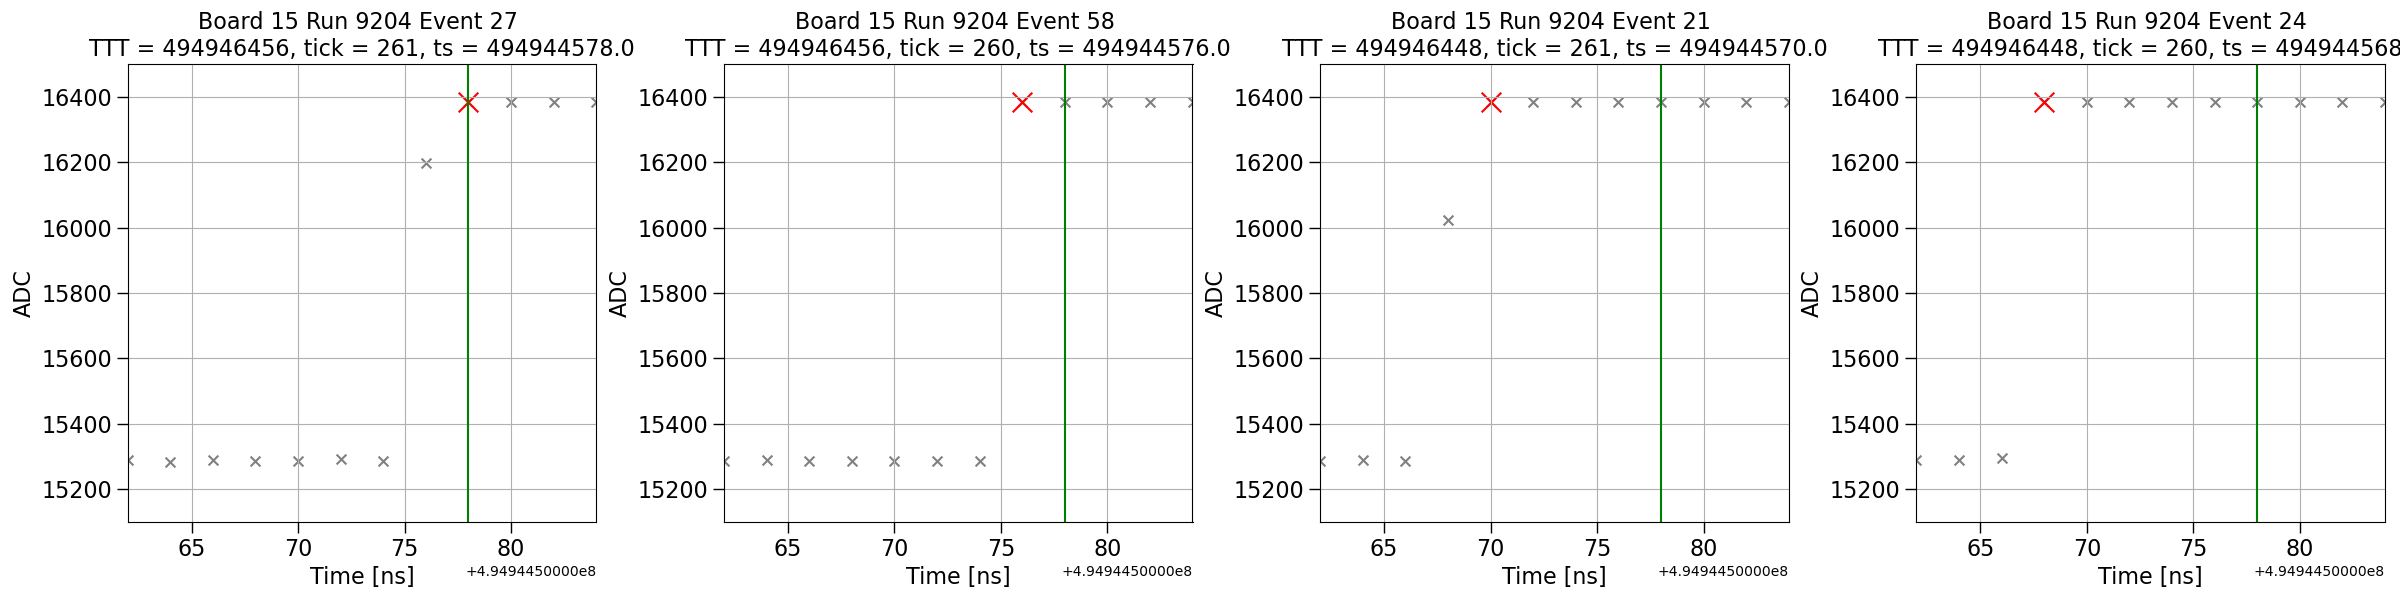
\includegraphics[width=\linewidth]{jitter_before}
\caption{Before Correction}
\label{subfig:jitter_before}
\end{subfigure}

\hfill
\begin{subfigure}[h]{1.00\linewidth}
\centering    
\includegraphics[width=\linewidth]{jitter_after}
\caption{After Correction}
\label{subfig:jitter_after}
\end{subfigure}%

\caption[jitterCorr]{
These plots show the zoomed in of the rising edge position of the trigger waveforms.
The far left plot show a synchronised event where no correction is needed for comparison.
For the rest of the plots from left to right, three cases of jittering are shown and their effects on both the TTT value and tick value of the rising edge.
The first case only contains the jittering of the ADC sampling clock, requiring a correction of 2 ns.
The second case only contains the jittering of the trigger clock, requiring a correction of 8 ns.
The third case contains the jittering from both of the clocks, thus the correction contains a combined smearing of 10 ns.
}
\label{fig:jitterCorr}
\end{figure}

\begin{figure}[htbp!]

\begin{subfigure}[h]{1.00\linewidth}
\centering    
\includegraphics[width=\linewidth]{Tickts_spec_corrEbyE}
\caption{After Correction Event By Event}
\label{subfig:Tickts_spec_corrEbyE}
\end{subfigure}

\hfill
\begin{subfigure}[h]{1.00\linewidth}
\centering    
\includegraphics[width=\linewidth]{Tickts_spec_corrRbyR}
\caption{After Correction Run by Run}
\label{subfig:Tickts_spec_corrRbyR}
\end{subfigure}%

\caption[jitterCorrEbyERbyR]{
The jittering correction to the tick-derived timestamp was applied in steps of event by event, followed by run by run.
This results in perfect synchronisation across all digitizers and with respect to the PPS signal.
Board 16 is an exception due to having different firmware. 
This jittering correction workflow still reveals the amount of correction for this board, which is -54 ns. 
An additional correction step can be taken to account for time synchronisation across digitizers with different firmwares. 
}
\label{fig:Tickts_spec_corr}
\end{figure}

%how to correct for jittering:
By digitising the trigger signal synchronously on every digitizer, the recorded waveform of the trigger provides all the necessary information to apply correction.
One can simply derive the correction amount by comparing the tick-derived timestamp of the trigger signal from one event to another, as illustrated in Fig. \ref{subfig:jitter_after}.
Once this correction is applied to all events within the same run, one can also correct for the random clock phase initialisation across multiple runs within the same CAEN digitizer.
This order of correction results in the perfect synchronisation across all events and all runs from different periods of time.
For demonstration, this correction workflow was applied to the distribution of the tick-derived timestamp previously shown in Fig. \ref{subfig:Tickts_spec}.
The correction was applied event by event followed by correction run by run as shown in Fig. \ref{fig:Tickts_spec_corr}, resulting in synchronisation across all the CAEN digitizers and also with respect to the PPS signal.

\begin{figure}[htbp!] 
\centering    
\includegraphics[width=0.6\textwidth]{pds_r0}
\caption[pdsR0]{
Photograph of the final set up for the PDS-R0 rack, which houses 8 CAEN digitizers for digitizing the PMTs, and a new addition 9th CAEN digitizers for digitizing the beam signals.
The daisy chain clock scheme is chosen, and channel 15 of every digitizer is input with the trigger signals to digitize the waveforms.
The waveform will contain necessary information for jittering correction in downstream analysis.
}
\label{fig:pdsR0}
\end{figure}

This study has resulted in a new hardware proposal by the author for physics run at SBND.
The proposal suggested to digitize the trigger signal in all channel 15 of every CAEN digitizer such that this will provide the necessary timing information for downstream jittering correction.
This new cable connection requires an additional CAEN digitizer since the original plan was to digitize beam signals in channel 15.
The new CAEN digitizer will be used solely for recording beam signals such as the BES and RWM signal.
The installation of the new hardware setup was carried out by the author during her time at Fermilab and this is photographed in Fig. \ref{fig:pdsR0}.


%********************************** %Third Section  **************************************
\section{Concluding Remarks}
\label{sec5Remarks}

The DAQ system of the SBND experiment has been outlined, detailing the overall process involved in constructing a physics event from various hardware subsystems. 
The event building process relies heavily on precise timing synchronization across these subsystems, achieved through the implementation of the WR timing system.
Each readout electronic device is synced with a PPS signal derived from the WR devices, ensuring that the timestamps of recorded events from each hardware component align with the frame of reference relative to the PPS signal.
The evaluation of the timing resolution of the readout electronics of the CRTs, which are the FEB modules, was presented. 
The timing resolution of the FEB modules was observed to be approximately 2 ns for both the T0 and T1 internal clocks.
Exploration into an alternative timing reconstruction method using timestamps from the T0 clock, combined with the SPEC-TDC, was undertaken. 
This method reconstructed the beam spill structure and substructure, demonstrating good agreement when compared to using timestamps from the T1 clock.
Additionally, an evaluation was conducted on the readout electronics for the PMTs, namely the CAEN digitizers, focusing on timing synchronization and resolution. 
The work resulted in the daisy chain clock scheme was chosen to synchronise all the digitizers within the same crate.
Furthermore, a method for jittering correction was devised by simultaneously digitising trigger waveforms in each digitizer. 
This correction method allows for absolute timing synchronization across all the CAEN digitizers as well as with the PPS signal up to resolution of 1 ns.



%!TEX root = ../thesis.tex
%*******************************************************************************
%****************************** Third Chapter **********************************
%*******************************************************************************
\chapter{Simulating SBND}
\label{ChapterSim}

% **************************** Define Graphics Path **************************
\ifpdf
    \graphicspath{{Chapter6/Figs/Raster/}{Chapter6/Figs/PDF/}{Chapter6/Figs/}}
\else
    \graphicspath{{Chapter6/Figs/Vector/}{Chapter6/Figs/}}
\fi

%********************************** %Opening  **************************************

%Modern physics experiments and MC
Many modern particle physics experiments heavily rely on simulations, of which many employ the Monte Carlo (MC) technique by random sampling from predefined distributions.
Simulation is particularly useful for an early stage experiment like SBND where the detector is not yet operational to record data.
Simulation enables studying of the physics capabilities of the detector as well as developing reconstruction and analysis tools in preparation for data.
The search for HNLs at SBND is an exploration of the detector physics capabilities in the BSM regime, given that the detector timing resolution can achieve nanosecond resolution.

The following chapter provides a detailed description of the simulation workflow at SBND to output simulated products that ideally represent real data.
The chapter begins with an overview of the workflow in Sec. \ref{sec:overview_sim}.
Meanwhile, Sec. \ref{sec:gen_mevprtl} includes the details of the generator employed to generate a signal event of HNLs and Sec. \ref{sec:gen_sm} provides the summary of the generators used to generate background events from SM neutrinos and cosmic muons.
Furthermore, details in Sec. \ref{sec:gen_response} follow the simulation of energy deposition as the particle propagates through the detector, and consequently the simulation of the detector response to the energy.
Finally, some concluding remarks are provided in Sec. \ref{sec:sim_concluding_remarks}.

\newpage

%********************************** %First Section  **************************************
\section{Overview of Simulating SBND}
\label{sec:overview_sim}

Similar to many other LArTPCs, the software framework for simulation, reconstruction and analysis of SBND is provided by the LArSoft framework \cite{larsoft}. 
The framework was built for neutrino experiments sharing the same common feature of having LArTPCs, while still allowing for detector-specific customisation. 
This enables easy sharing of software tools across many collaborations including ArgoNeuT, MicroBooNE, ICARUS, SBND and DUNE. 
For example, the generator used to simulate HNLs, to be discussed in the next section, has been developed and shared across the SBND and ICARUS collaboration.

%Describe the overall workflow
The simulation workflow of SBND under the LArSoft framework is depicted in Fig. \ref{fig:Sim_Workflow}.
The process begins with a generator to produce primary particles that enter the detector, as shown by the purple box.
The primary particles can be neutrinos, cosmic muons or BSM particles depending on the type of generator.
The propagation of the primary particle inside and outside the detector, and the resulting energy deposition is simulated using the Geant4 tool kit \cite{geant4}, as shown by the green boxes.
For interactions inside the detector, the charge and light yield are calculated from the energy deposition.
Ionisation electrons from the charge yield are propagated through the detector to the wire planes using the Wirecell tool kit \cite{wirecell}, as shown by the red boxes.
Scintillation photons from the light yield are propagated to the photodetectors using a combination of semi-analytical model and light library \cite{sbnd_pds_paper}, as shown by the blue boxes.
For interactions outside of the detector, only the energy depositions within the CRT strips are converted into light yield, as shown by the orange box.
The detector response is then simulated for each detector subsystem.
By the end of this stage, the outputs from each detection subsystem ideally represent real data.

\begin{figure}[htbp!] 
\centering    
\includegraphics[width=1.0\textwidth]{Sim_Workflow}
\caption[Sim_Workflow]{
Overview of the simulation workflow of the SBND detector.
}
\label{fig:Sim_Workflow}
\end{figure}

\section{HNL Generator: MeVPrtl}
\label{sec:gen_mevprtl}

%MeVPrtl Workflow
MeVPrtl was developed as a modular generator, allowing for easy adaptations for different beam sources and detectors, as well as a direct interface with the existing LArSoft framework.
The workflow of the MeVPrtl is broken down into 4 stages, as illustrated in Fig. \ref{fig:MeVPrtl_Workflow}.
The generator begins with taking an input of meson fluxes, representing the particles produced from a beam source.
It then simulates the meson decaying to a BSM particle.
The BSM particle is propagated to the detector and decays back into SM observables.
There are several BSM models already implemented in the MeVPrtl generator, including HNLs, Higgs portal scalars \cite{higgs_scalar} and heavy QCD axions \cite{qcd_axion}.

\begin{figure}[htbp!] 
\centering    
\includegraphics[width=1.0\textwidth]{MeVPrtl_Workflow}
\caption[MeVPrtl_Workflow]{
Overview of the workflow of the MeVPrtl generator.
}
\label{fig:MeVPrtl_Workflow}
\end{figure}

%Each stage validation
For generating HNLs coming from the BNB, the generator begins with sampling the $K^{+}$ fluxes of the BNB.
Instead of decaying into SM neutrinos, the kaons decay either in-flight or at rest into HNLs, with the branching ratio defined by Eq. \ref{eq:kaon_decay_hnl}.
The daughter HNL and lepton are simulated using the two-body decay at rest in the centre of mass frame of the parent kaon and then boosted to the parent's lab frame by Lorentz boost.
Due to HNLs having mass, HNLs have less transverse momentum than SM neutrinos and therefore are more collimated, travelling preferably to the parent kaon direction.
The Lorentz boost can flip the directions of HNLs that are emitted backwards, originating from low energy kaons \cite{DavidePhD}.
HNLs are propagated to the detector by the ray tracing method, which forces HNLs to hit the SBND detector by picking a direction that impinges the particles at the detector's front face.  
The probability of enforcing the detector intersection is also computed.
Example angular distributions in the lab frame of parent kaons and HNLs that arrive at the SBND detector are shown in Fig. \ref{fig:kaon_hnl_angle2beam}.
For plotting completeness, the plotted parent kaons have energies peaking approximately $0.5\sim1$ GeV and are evenly distributed in the angle with respect to the beam direction, as shown in Fig. \ref{fig:kaon_angle2beam}.
The resulting HNLs of mass 240 MeV and their angles to the beam direction are shown in Fig. \ref{fig:hnl_angle2beam}.
This demonstrates that the acceptance angle of the HNLs to hit the SBND detector is very small ($\theta < 5^\circ$), such that only very forward-going HNLs are most likely to intersect the detector.

\begin{figure}[htbp!]
        \centering
        \begin{subfigure}[b]{0.495\textwidth}
            \centering
            \includegraphics[width=\textwidth]{kaon_angle}
            \caption{Kaons}%
            \label{fig:kaon_angle2beam}
        \end{subfigure}
        \hfill
        \begin{subfigure}[b]{0.495\textwidth}  
            \centering 
            \includegraphics[width=\textwidth]{hnl_angle}
            \caption{HNLs}%
            \label{fig:hnl_angle2beam}
        \end{subfigure}
        \caption[kaon_hnl_angle2beam]{Example distributions of angle to the beam direction, for the parent kaons and for the resulting HNLs that arrive at the detector.}
        \label{fig:kaon_hnl_angle2beam}
\end{figure}

The resulting fluxes of HNLs arriving at the SBND detector are depicted in Fig. \ref{fig:HNL_Energy_Spectrum} for the mass range between 140 and 240 MeV.
The fluxes are normalised to the same mixing angle $|U_{\mu4}|^{2} = 1 \times 10^{-7}$ and 3 years of data taking, equivalent to $1 \times 10^{21}$ POT.
At the same mixing angle, the expected HNL rate decreases with lower mass since the branching ratio of $N \rightarrow \nu\pi^0$ decreases with lower mass, as previously shown in Fig. \ref{fig:branchingRatio}.
Since the $K^{+}$ flux peaks around 0.5 GeV and decreases at higher energy, as previously shown in Fig. \ref{fig:BNB_Meson_Flux}, the HNL fluxes also mainly concentrate in the low energy region, and substantially decrease at higher energy. 
Moreover, across the HNL mass range, there are more energetic HNLs at a lower mass than at a higher mass.
This is due to HNLs coming from a kaon decay and therefore, the lighter the HNL mass, the more kinetic energy is available.
Finally, all the HNL fluxes have a sharp peak near zero, corresponding to HNLs resulting from Kaons Decay At Rest (KDAR).

Once arrive at the detector, HNLs decays back into the SM observables.
For the $\nu\pi^{0}$ final state, the width of the decay is defined by Eq. \ref{eq:pi0}.
\begin{figure}[tbp!] 
\centering    
\includegraphics[width=0.65\textwidth]{HNL_Energy_Spectrum}
\caption[HNL_Energy_Spectrum]{
Simulated HNL fluxes for mass ranging from 140 to 240 MeV, normalised to the mixing angle $|U_{\mu4}|^{2} = 1 \times 10^{-7}$ and $1 \times 10^{21}$ POT.
}
\label{fig:HNL_Energy_Spectrum}

%\end{figure}
%\begin{figure}[bp!]

        \centering
        \begin{subfigure}[b]{0.495\textwidth}
            \centering
            \includegraphics[width=\textwidth]{pi0_energy}
            \caption{Energy Distribution}%
            %\label{fig:kaon_angle2beam}
        \end{subfigure}
        \hfill
        \begin{subfigure}[b]{0.495\textwidth}  
            \centering 
            \includegraphics[width=\textwidth]{pi0_angle2Beam}
            \caption{Angle to the Beam Direction Distribution}%
            %\label{fig:hnl_angle2beam}
        \end{subfigure}
        \caption[pi0_distribution]{Kinematic distributions for neutral pions resulting from HNLs decaying inside the SBND detector.}
        \label{fig:pi0_distribution}
\end{figure}
The kinematics of the decay products are simulated for HNLs isotropically decay in the rest frame and then boosted to the lab frame by Lorentz boost.
Since the parent HNL is very forward-going, the daughter $\pi^0$ is also forward-going, with momenta dependency on the mass of the parent HNL. 
Fig \ref{fig:pi0_distribution} shows the energy and angle to the beam distributions for the daughter $\pi^0$.
The plots are area-normalised for comparison across the mass range of the parent HNL from 140 to 240 MeV. 
The peak in the energy distribution at low energy and the peak in the angular distribution at high angle are from the $\pi^0$ coming from low energy HNLs from KDAR.
The energy distribution of the $\pi^0$ decreases as the HNL mass increases since heavier HNLs are less energetic and therefore, less energy available for the $\pi^0$.
As a result, the angle to the beam of the $\pi^0$ also widens with heavier HNLs.
However, at the heaviest HNL mass of 240 MeV considered in the search, the $\pi^0$ is still very collimated with angular distribution dominating in the region $< 30^\circ$. 
Therefore, the di-photon showers from the HNL-originated $\pi^0$ are expected to be more forward-going than those originate from SM neutrinos.

%Timing
One key motivation of the HNL search is the timing delay between HNLs compared to SM neutrinos, due to HNLs being more massive.
The total time of flight for a HNL or a SM neutrino produced from the BNB and propagates to the SBND detector is illustrated in Fig. \ref{fig:tof_beam_to_detector}.
The first component is the spill time of the protons from the Booster synchrotron, $t_{spill}$, as shown by the red arrow.
The structure of $t_{spill}$ is the beam bucket structure made up of 81 Gaussian buckets with a width of 1.308 ns and a spacing of 19 ns, which is the same for both HNLs and SM neutrinos.
Details of the beam structure was previously detailed in Sec. \ref{sec4BNB}.   

\begin{figure}[htbp!] 
\centering    
\includegraphics[width=1.0\textwidth]{tof_beam_to_detector}
\caption[tof_beam_to_detector]{
Diagram of the time of flight for a SM neutrino or a HNL, starting from the Booster synchrotron until the interaction time inside the SBND detector.
}
\label{fig:tof_beam_to_detector}
\end{figure}

The second component is the time of the secondary mesons, $t_{meson}$, as shown by the blue arrow.
This the time period from when the mesons are produced until they decay into HNLs or SM neutrinos.
This time accounts for the time the mesons travel down the decay pipe, and might interact, re-scatter or decay into other mesons.
In the case of HNLs, $t_{meson}$ is primarily the time of flight of the charged kaon $K^+$ before decaying into a HNL.
On the other hand, SM neutrinos come from a variety of parent mesons $t_{meson}$, previously listed in Fig. \ref{fig:BNB_neutrino_flux}.
In both cases, $t_{meson}$ introduces some smearing to the nanosecond-bucket structure of $t_{spill}$.

The last component is the time of flight of the SM neutrino or the HNL from the creation point to the interaction point inside the SBND detector.
In the case of SM neutrinos, since they are nearly massless, their velocity can be approximated as the speed of light. 
Then, the time of flight of the SM neutrino is  
\begin{equation}
	t_{\nu} = \frac{d_{\nu}}{c}
\end{equation}
where $d_{\nu}$ is the distance of a neutrino from the creation point to the interaction point inside the detector.
Meanwhile, HNLs are massive and therefore, travel at a velocity $v_N < c$.
The time of flight of the HNL is
\begin{equation}
	t_{N} = \frac{d_{N}}{v_N}
\end{equation}
where $d_N$ is the distance of a HNL from the creation point to the decay point inside the detector.
Additionally, since the energy of the HNL decreases with its mass, the heavier it is, the slower its velocity.
Thus, heavier HNLs arrive even later compared to lighter HNLs.

The advantage of the MeVPrtl generator is the consistency of simulating the time of flight of HNLs similar to how the GENIE generator simulates SM neutrino.
Fig. \ref{fig:full_beam} shows the arrival time of SM neutrinos and 240 MeV HNLs at the front face of the SBND detector, recovering the beam spill structure of the BNB.
The plot is area-normalised to enable the comparison between the two particles. 
Since SM neutrinos travel nearly at the speed of light, less smearing is introduced and the timing distribution shows sharp Gaussian peaks.
On the other hand, HNLs travel slower and therefore, add additional smearing and delay tails to the Gaussian peaks.
For clarity, 81 Gaussian peaks are overlaid into one by taking the modulus of 19 ns, as shown in Fig. \ref{fig:beam_modulus}.
The timing distribution of the HNLs shows a clear distinction from that of SM neutrinos, where delay tails on either side of the Gaussian peak can be seen.
Across the mass range of HNL from 140 to 240 MeV, the delay tails however do not increase significantly with mass.

\begin{figure}[htbp!] 
\centering    
\includegraphics[width=1.0\textwidth]{full_beam}
\caption[full_beam]{
Distribution of the arrival time at the front face of the SBND detector for SM neutrinos simulated by the GENIE generator and for HNLs simulated by the MeVPrtl generator. 
}
\label{fig:full_beam}
\end{figure}
\begin{figure}[htbp!] 
\centering    
\includegraphics[width=0.55\textwidth]{beam_modulus}
\caption[beam_modulus]{
Modulus of the of arrival time distribution of SM neutrinos and HNLs with mass ranging from 140 to 240 MeV. 
}
\label{fig:beam_modulus}
\end{figure}

\newpage
\section{Other SM Generators}
\label{sec:gen_sm}

\subsection{Neutrino Generator: GENIE}
\label{sec:gen_genie}

%Overview of GENIE
SM neutrino interactions are generated by the GENIE generator \cite{genie}, which provides a selection of theoretical and empirical models for different physical processes.
These models can be combined into a \textit{tune} by comparing predictions to data from neutrino and electron scattering experiments.
The SBND collaboration is planning to use a tune that was specifically developed to serve as a baseline model for the SBN and DUNE oscillation analysis.
Details for the basis of the tune can be found in Table 1 in Ref. \cite{genie_tune}, with ongoing developments on the choice of models documented in Ref. \cite{genie_tune_github}.  

%What kind of tune are being used
In general, GENIE first selects a nuclear model that describes the momenta and potential energy of the nucleon to model nuclear effects.                                                                                           
Then, the neutrino flux and the integrated cross-section model are used to compute the probability that a neutrino interaction occurs.
The differential cross-section is then used to determine the type of neutrino interaction and the kinematic range.
The neutrino interaction types include Quasi-Elastic (QE), Baryonic Resonant Scattering (RES), Coherent Scattering (COH), Deep Inelastic Scattering and $\nu$-e elastic scattering.
DIS interactions can additionally produce hadrons within the nuclei, which these hadrons can propagate through the nucleus and modify the observed kinematics.
Thus, the Final State Interaction (FSI) model is crucially important for predicting the observable topology of neutrino interactions since argon is a heavy nuclear target.

In addition to the tune, GENIE also provides a re-weighting scheme to evaluate the systematic uncertainties for a model chosen in the tune.
Due to the scarcity of neutrino interaction data, particularly for $\nu-Ar$ interactions, the uncertainties in cross-section modelling tend to be large and can hamper the capabilities of the HNL sensitivity.  
The neutrino interaction re-weighting scheme and the resulting systematics uncertainties impact on the HNL search will be discussed in detail in Sec. \ref{}.

GENIE simulates neutrino interactions occurring both inside and outside of the detector volume, with a boundary defined in Fig. \ref{fig:Rockbox_Volume}.  
All interactions occurring inside the detector volume are strictly kept, as shown by the dark blue box.
Outside of the detector, a buffer volume is defined as 5 m surrounding the detector volume, as shown by the light blue box.                       
An additional Rockbox volume is defined by extending the buffer volume backwards in the beam direction ($z$-axis) up to 15 m in front of the buffer volume, as shown by the orange box.
Both these volumes are referred to together as the \textit{Rockbox} volume in this thesis.
Neutrino interactions within this volume are kept, whose products can potentially deposit energy in the detector.
These interactions are referred to as \textit{dirt} neutrinos and constitute a significant background to the HNL search.
The background rejection of dirt neutrinos will be covered in Chapter \ref{ChapterSelect}.

\begin{figure}[htbp!] 
\centering    
\includegraphics[width=0.85\textwidth]{Rockbox_Volume}
\caption[Rockbox_Volume]{
Diagram showing the volume boundary defined by the GENIE generator to simulate neutrino interactions occurring inside and outside of the detector volume. 
}
\label{fig:Rockbox_Volume}
\end{figure}

\subsection{Cosmic Generator: CORSIKA}
\label{sec:gen_corsika}

%how corsika generator works
Cosmic interactions are simulated using the CORSIKA generator \cite{corsika}.
The generation begins with producing high energy primary particles incident in the Earth's atmosphere, of which only primary protons are kept. 
The primaries are then propagated through the atmosphere, interacting with the air to produce secondary decays until reaching the Earth's surface.
Within the SBND simulation geometry, this surface is specified to be just above the roof of the detector building.
The surviving particles are then propagated to the SBND detector.

%Why cosmic simulation is important
From a triggering perspective, there are two types of comic muons as follows 
\begin{itemize}
        \item\textbf{In-time} cosmic muons cross the detector at the same as SM neutrinos being present inside the detector, such that the muons are \textit{inside} the beam spill window. The cosmic muons produce enough light to
 induce a beam trigger.                            
        \item\textbf{Out-of-time} cosmic muons occur regardless of the trigger conditions. The muons cross the detector \textit{outside} the beam spill window but within the readout window.  
\end{itemize}
However, triggering is currently not being simulated in the workflow. 
Only the timing requirement is simulated to keep only cosmic muons occurring within the readout window.
The simulation currently does not accurately reflect the cosmic rate once factoring triggering conditions and therefore, comparison to data is necessary. 

Being a surface-level detector, it is vitally important to understand the cosmic background at SBND due to the exposure to a high cosmic rate.
Once SBND is operational, a particularly useful measurement is the rate of cosmic muons that cause a beam trigger, however, in the absence of the beam.
This is equivalent to measuring the rate of cosmic muons that produce sufficient energy inside the detector to mimic SM neutrino interactions.
This measurement allows for validation against the CORSIKA generator sampling of the cosmic topology and kinematic distribution. 
Moreover, it also provides an expected cosmic rate given a triggering condition, which can be subsequently added to the simulation workflow to better constrain the cosmic background.                   

\section{Particle Propagation and Detector Response Simulation}
\label{sec:gen_response}

\subsection{Particle Propagation Simulation}
\label{sec:gen_g4}

Once a particle is simulated inside the detector, it is propagated through the detector using the Geant4 tool kit \cite{geant4}.
Geant4 propagates the particle by each step $dx$, where the step length is randomised and capped at 0.3 mm (one order of magnitude less than the wire pitch).
At each step, physics processes are applied to the particle, such as energy deposition, interaction, decay and so on.
The step propagation also accounts for the electric field distortion caused by the space charge effect due to a high exposure to cosmic muons.
For example of the $\nu\pi^0$ final state of HNLs, the $\nu$ escapes the detector without interacting while the $\pi^0$ is simulated to decay into a di-photon shower by Geant4.
Then, Geant4 simulates the energy deposition of the resulting di-photon shower.

The main physics process for energy deposition in the detector is ionisation by charged particles.
Similarly to the theory detailed in Sec. \ref{sec3:creation}, the Geant4 tool kit simulates the ionisation process following the Bethe-Bloch formalism tuned to data \cite{geant4_ions}.
The number of ionisation electrons and scintillation photons from the deposited energy is computed using the ModBox recombination model with ArgoNeuT parameters \cite{argoneut_recomb}, and the charge-light anti-correlation from Eq. \ref{eq:Q} and \ref{eq:L}. 
Further discussion about the simulation of recombination, and the impacts of delta ray fluctuations on recombination will be detailed in the forthcoming Sec. \ref{sec7:delta}.
The result from the Geant4 tool kit is a complete set of charge and light yields along the primary particle trajectories through the detector and the hierarchy of the daughter particles produced from the primary.

\subsection{Wire Response}

The charge yield, or the number of ionisation electrons, is simulated to drift towards the wire planes by the WireCell tool kit \cite{wirecell}.
The simulation transports the electrons and introduces smearing due to detector effects for transporting electrons through liquid argon under an electric field, which is previously discussed in Sec. \ref{sec:edrift}.
This includes charge attenuation due to impurities, smearing of the electron deposition in timing and spatial dimensions due to longitudinal diffusion, transverse diffusion and space charge effect combined.

Once drifting electrons arrive at the wire planes, a convolution of the field response and the electronic response is performed.                                                                                                          
The field response describes the current induced on wires due to ionisation electrons drifting past the induction planes.                                                                                                           
The electronic response describes the amplification and shaping by pre-amplifiers of wires.                 
The response functions are in two dimensions, one dimension is in time and the other is in wire.
This is to account for the long-range charge induction effect on wire signal shapes.
A digitisation step is then applied to produce an ADC-level, time-domain waveform for each wire channel.
The waveform is parameterised by the ADC resolution, voltage range and baseline specification of the wire readouts. 
Finally, inherent electronic noise is added to the waveform to better match to observed data.
MC waveforms at this stage ideally represent real data waveforms recorded by the wire readouts.

\subsection{PDS Response}

Scintillation photons from energy deposition are simulated to propagate to to optical detectors, accounting for transport effects previously detailed in Sec. \ref{sec:photonprop} such as Rayleigh scattering and boundary effects.
The simulation uses a combination of semi-analytical model described in Ref. \cite{pds_sim}, and optical library model available in LArSoft.
The choice of which model to use depends on the location of the photon production.
The semi-analytical model is used for those produced inside the active volume of the SBND detector, whilst the optical library model is used to those originate outside of this volume.
In-depth details of the light simulation can be found in Ref. \cite{sbnd_pds_paper}.

The semi-analytical model calculates on-the-flight the geometrical aperture for each optical detector to a scintillation point, given that the emission of scintillation photons is isotropic.
The model also extends to both direct visible photons and also reflected VUV photons. 
Corrections for photon transport effects are applied to the number of photons detected by an optical detector.
However, the semi-analytical method is limited by the geometrical information and does not include scintillation outside of the detector volume, for example, cosmic muons crossing behind an optical detector can produce non-negligible photons.
Since PMTs are the primary subsystems for triggering, it is vital to consider this second-order contribution of photons for triggering studies.
The optical library stores information of the fraction of incident photons for each optical detector for a given scintillation location, which can be looked up for any detector-location pairs during simulation. 

For each type of optical detector, PMTs and X-ARAPUCAs, a respective photon detection efficiency is applied to the number of detected photons.
Then, signal amplification and digitization are simulated, converting photons into an output signal known as a single electron response.
Signal shaping such as overshoot and undershoot due to the AC circuit of the optical detectors are also simulated.
Finally, random fluctuation in the signal integral and non-linearity response at high light intensities are applied to better mimic data.
The final output is MC optical waveforms for each type of optical detector, ideally the same as data. 

\subsection{Cosmic Ray Tagger Response}

The energy deposition outside of the cryostat from the Geant4 simulation stage in Sec. \ref{sec:gen_g4} is considered if it crosses the CRT strips.
The energy is converted into the light yield within a strip and then propagated down optical fibres towards the SiPMs.
The collection efficiency per SiPM is accounted for by dividing the light yield between the fibres on either side of the strip, based on the lateral position of the energy deposition within the strip.
Propagation effects and signal attenuation are also simulated.
Finally, the electronic response is simulated for the CRT readout, by assessing if a pair of SiPMs within a strip goes above a threshold within a pre-defined coincidence window.
The MC output is in group of 32 SiPMs, consisting of a single ADC value per SiPM.

\section{Concluding Remarks}
\label{sec:sim_concluding_remarks}

The simulation framework of SBND described here shares the same purpose as with many other modern particle physics experiments, to help understand and improve the detector performance and physics capabilities.
This is done by simulating the end-to-end process from when a particle is produced, to how it deposits energy inside the detector and consequently, the detector response to the energy deposition.
The MC output of the simulation ideally mimics data, providing the foundation to perform different types of exploratory studies before SBND becomes operational.
For example, the upcoming Chapter \ref{ChapterReco} will provide a description of the reconstruction framework at SBND, of which many algorithms have been developed using MC samples.
Furthermore, the calibration studies presented in Chapter \ref{ChapterCalib} were carried out using MC samples of protons and muons to better understand particle-dependent energy deposition.
Finally, the search on HNLs presented in the two final Chapter \ref{ChapterSelect} and \ref{ChapterResult} was also performed using MC samples to explore the capability of SBND in the BSM regime.


%!TEX root = ../thesis.tex
%*******************************************************************************
%****************************** Third Chapter **********************************
%*******************************************************************************
\chapter{Reconstructing SBND}
\label{ChapterReco}

% **************************** Define Graphics Path **************************
\ifpdf
    \graphicspath{{Chapter7/Figs/Raster/}{Chapter7/Figs/PDF/}{Chapter7/Figs/}}
\else
    \graphicspath{{Chapter7/Figs/Vector/}{Chapter7/Figs/}}
\fi

%********************************** %Opening  **************************************

Reconstruction is the process of extracting physics quantities from the raw detector data.
For SBND, the goal of reconstruction is to reconstruct particles that deposit energy within the detection subsystems.
A contained particle inside the TPC might deposit energy resulting in only waveforms recorded by the TPC wire planes and the PDS, meanwhile, an exiting particle might deposit additional energy in CRT walls surrounding the TPC.
For a given particle, the TPC reconstruction can extract various quantities describing its topology, calorimetry and kinematics.
The PDS reconstruction can provide additional high resolution timing information of the particle on the top of its light calorimetry.
The CRT reconstruction can indicate if the particle is fully contained inside the detector.
As a result, the reconstruction variables from all three detection subsystems are complementary to each other and can be exploited for different analysis purposes such as cosmic rejection or particle identification.

This chapter provides a summary of the reconstruction framework at SBND.
The first Sec. \ref{sec:reco_overview} gives an overview of the reconstruction workflow for each detection subsystem. 
The following Sec. \ref{sec:reco_tpc} provides the details of the TPC reconstruction workflow from start to end.
Meanwhile, the reconstruction of the PDS and CRT subsystem are summarised in Sec. \ref{sec:reco_others}.
Furthermore, descriptions of some high-level analysis tools using the reconstruction variables collectively from each detection subsystem are included in Sec. \ref{sec:reco_ana_tools}.                 
Finally, the chapter is concluded in Sec. \ref{sec:reco_concluding_remarks} with some remarks.

\newpage

%********************************** %First Section  **************************************

\section{Overview of Reconstructing SBND}
\label{sec:reco_overview}

%Describe the overall workflow
Each detection subsystem in SBND requires a dedicated reconstruction workflow.
An overview of each workflow is illustrated in Fig. \ref{fig:Reco_Workflow}.
The TPC reconstruction workflow is shown by the red boxes.
This process begins with raw wire waveforms going through the signal processing performed by the Wirecell tool kit \cite{wirecell}.
This is followed by a hit finding algorithm to identify hits on the waveform.
Output hits are then used by the Pandora package \cite{pandora} to produce a 3D-reconstructed interaction, denoted as a \textit{slice}.
The PDS reconstruction workflow also follows a similar process to the TPC, as shown by the blue boxes.
A waveform deconvolution is first performed on raw PDS waveforms to filter noise.
Then, a hit finding algorithm identifies optical hits on the waveform and reconstruction is performed on the hits.
The equivalent output to the TPC-reconstructed interaction from the PDS reconstruction is referred to as a \textit{flash}.
Finally, the reconstruction for the CRTs is much simpler compared to the other two subsystems, consisting of only a hit finding and a reconstruction algorithm, as shown by the orange boxes.
The reconstruction variables from each detection subsystem are produced independently and can be matched together if they originate from the same interaction. 
The variables can also be combined and input into different high-level analysis tools to extract more
 complex properties of the underlying interaction. 

\begin{figure}[htbp!] 
\centering    
\includegraphics[width=1.0\textwidth]{Reco_Workflow}
\caption[Reco_Workflow]{
Overview of the reconstruction workflow of the SBND detector.
}
\label{fig:Reco_Workflow}
\end{figure}

\newpage
\section{TPC Reconstruction}
\label{sec:reco_tpc}

\subsection{TPC Signal Processing}
%Signal Processing
Signal processing is the first crucial step of TPC reconstruction, which is to deconvolve digitised raw waveforms and remove detector effects such as noise, electronics response and field response. 
At SBND, signal processing is implemented using the WireCell tool kit \cite{wirecell}.
The tool has been used by other various LArTPC experiments such as MicroBooNE and ProtoDUNE and has demonstrated excellent performance to acquire deconvolved charge by performing deconvolution in time and wire dimension over the traditional deconvolution in time dimension only. 

Fig. \ref{fig:signal_processing_steps} \cite{LynnSignal} demonstrates the step by step of the signal processing.
In grey is the true charge deposition on a wire, and in red is the corresponding raw waveform containing the signal convolved with noise, electronics response, field response and noise.
The first step in the chain is noise filtering to remove the excess and correlated noise from raw waveforms.
Then, the measured charge is deconvolved from the electronics and field response to recover the original charge deposited on the wire, as shown in orange.
The deconvolution is 2D, where response functions consider the time response of a single wire as well as the responses of neighbouring wires.
This step is particularly important for the induction planes to convert bipolar into unipolar signals, such that the integral of the waveform can be used for charge estimation.
\begin{figure}[tbp!] 
\centering    
\includegraphics[width=0.45\textwidth]{signal_processing_steps}
\caption[signal_processing_steps]{
Example demonstrating the steps of signal processing applied to a bipolar raw waveform.
Fig. from Ref. \cite{LynnSignal}.
}
\label{fig:signal_processing_steps}
%\end{figure}
%\begin{figure}[htbp!]
\vspace{1cm}
\centering    
\includegraphics[width=0.75\textwidth]{signal_processing_waveform}
\caption[signal_processing_waveform]{
Event display of a simulated neutrino event using true ionisation charges (left), raw waveforms (middle) and deconvolved waveforms (right).
Fig. from Ref. \cite{LynnSignal}.
}
\label{fig:signal_processing_waveform}
\end{figure}
Filter functions are applied subsequently to attenuate noise that is artificially amplified.
This includes high frequency filters to remove high frequency noise, whereas Gaussian or Weiner filters can be used depending on whether the signal is unipolar or bipolar.
The example shown here is a bipolar signal waveform and therefore has both Gaussian and Weiner filters applied.
Then, low frequency filters are utilised for region-of-interest finding and local baseline removal, as shown in blue.
Finally, the deconvolved waveform per wire after baseline removal is shown in purple.

Fig. \ref{fig:signal_processing_waveform} depicts event displays of a simulated neutrino event as recorded by wires on the u plane.
The left figure displays the event using true charge depositions on wires.
The middle figure shows the event using raw waveforms, whilst the right figure shows the same event using deconvolved waveforms.
Recently, the deconvolution and filtering algorithms have been optimised specifically for the SBND detector.
This is demonstrated in the right event display showing clean signals.
Two tracks and two showers can be observed, closely resemblance the true charge deposition. 

\subsection{TPC Hit Finding}

After signal processing, hit finding is performed on deconvolved waveforms to search for Gaussian-shaped pulses above a threshold.
This is done by the \texttt{GausHitFinder} module \cite{gaushitfinder} by fitting a series of Gaussians to the waveform.                                                                                  
The number of pulses is determined by the number of maxima found when differentiating the waveform, where each pulse represents a hit.                                                                   
Fig. \ref{fig:gaushit} \cite{EdPhD} demonstrates the hit finding process for a deconvolved waveform, showing four hits have been identified and fitted with a Gaussian.
Once the hits are fitted, information describing the hit is extracted and used by downstream pattern recognition and reconstruction.
The peak time represents the time at which the charge arrives at the wire, used for determining the drift position and matching hit coincidence across wire planes.
The height and the width of the Gaussian are used to calculate the integral of the pulse, representing the deposited charge on the wire, subsequently used in downstream analysis for calorimetry computation.

\begin{figure}[htbp!] 
\centering    
\includegraphics[width=0.5\textwidth]{gaushit}
\caption[gaushit]{
Diagram illustrating the hit finding algorithm performance on a single wire.
Fig. from Ref. \cite{EdPhD}.
}
\label{fig:gaushit}
\end{figure}

\subsection{Pandora Pattern Recognition}

%Pattern Recognition: Pandora
The output hits from the hit finding process are then used to perform 3D reconstruction, which is performed with the Pandora pattern recognition package\cite{pandora}.
The package was first developed for the International Linear Collider and later extended to other LArTPC experiments.
It is made up of over 100 individual algorithms, performing a specific task along the reconstruction chain.
The output from Pandora represents an interaction, containing a hierarchy of particles starting with a neutrino parent at the interaction vertex.
This reconstructed object is referred to as a \textit{slice}.

The reconstruction begins with a workflow to reconstruct cosmic-like objects that leave long tracks inside the detector.
This workflow performs a 2D clustering on each wire plane independently, followed by 3D reconstruction under the assumption that all clusters are track-like.
Then, a cosmic rejection is performed to identify if a cluster is cosmic-like or neutrino-like.
The cosmic removal at this stage is deliberately cautious such that only very unambiguous cosmic muons in nature are removed.

The remaining clusters are then input into a second workflow dedicated towards neutrino reconstruction.
This workflow begins with a slicing algorithm that divides clusters into \textit{slices}, where each slice encapsulates hits coming from a single origin, representing an interaction.
Then, 2D clustering is re-performed on each wire plane independently, however, with a new assumption that clusters can be both track-like and shower-like.
A vertexing algorithm then identifies the interaction vertex of the slice and its associated clusters.
A series of pattern matching algorithms grows the interaction out of the neutrino vertex and performs 3D reconstruction by matching 2D clusters across different planes.
The output 3D reconstructed object associated with a vertex ideally represents a \textit{particle} produced from an interaction.

At this stage, a \textit{track score} is assigned to a particle if it has a track-like or a shower-like topology, which is determined by a dedicated Boosted Decision Tree (BDT).
The development work on the track-shower separation BDT and its importance not only in the reconstruction workflow but also in the analysis workflow will be covered in the next Sec. \ref{sec:trkshwbdt}.
Both track and shower reconstruction tools are then performed on the particle. 
Finally, a hierarchy algorithm is performed to classify the hierarchy of particles in a slice, starting with a neutrino parent vertex, and other particles are children, grandchildren, etc. of the parent.                             

%Calorimetry reconstruction
The last stage of reconstruction is calorimetry computation for the output slices and their associated particles.
Both track and shower calorimetry computations first convert ADC units to charges, or number of electrons, via multiplying by a charge calibration constant.
The track calorimetry then computes the energy from the charge using the ModBox recombination formalism, factoring in the electric field distortion.
Meanwhile, the shower calorimetry reconstruction converts the measured charge to energy by multiplying it by a shower calibration constant, factoring in an averaged recombination factor. 
Once the SBND detector is operational, the calibration constants will be measured via dedicated calibration physics runs.
The charge calibration constant is expected to be computed by using a sample of the anode to cathode crossing muon tracks while the shower calibration constant can be acquired from using a standard candle of the neutral pion invariant mass \cite{uboone_gamma}.

\subsection{Track-Shower Separation Boosted Decision Tree}
\label{sec:trkshwbdt}
As previously discussed, reconstructed particles from Pandora are assigned with a track score determined by Boosted Decision Tree (BDT), which is a binary classification machine learning tool.
The track score spans between 0 and 1 such that if a particle has a very high track score close to 1, then the particle is track-like.
Otherwise, if the track score is very close to 0, then the particle is shower-like.

The track-shower BDT has become more important in the reconstruction as well as the analysis workflow due to a new reconstruction paradigm introduced by Pandora.
The traditional reconstruction approach was to perform only either track or shower reconstruction on a particle based on its track score.
Meanwhile, the new paradigm performs both track and shower reconstruction on a particle regardless of the track score.
All reconstructed particles now have two sets of reconstruction variables for track-like and shower-like.
The users have the freedom to decide which variables to use depending on their signal topology, and thus not pre-determined by Pandora.
The track score can inform on which appropriate reconstruction variables should be used for the analysis. 

The track-shower separation BDT was trained on a series of reconstruction variables and was updated to include new variables in the training.
The original BDT includes variables describing the geometrical topology of the particle such as its length, distance and direction with respect to the parent vertex, as well as calorimetry variables describing the charge distribution of the particle.
More details of the input variables and the training of the BDT can be found in Ref. \cite{EdPhD}.
The update extended beyond the original work to include a brand new set of variables describing how cone-like the charge distribution of a particle as well as a new variable describing the particle hierarchy.

The cone variables were first developed by the M. Haigh for particle identification \cite{warwick_pid}, and now imported into Pandora for reconstruction purposes.
There are three variables: (1) halo-total ratio, (2) concentration and (3) conicalness as depicted in Fig. \ref{fig:cone_variables}.
The diagrams depict the hit distribution of a hypothetical particle, where each circle represents a hit associated with a charge value and the star represents the vertex of the hit cluster.
The illustration is in 2D however the variables are computed in 3D.
The first variable is the halo-total ratio, illustrated in Fig. \ref{fig:halototalratio}.
The region outside of the Moliere radius, defined such that 90\% of the cluster energy is contained within this radius, is considered the halo region.
\begin{figure}[bp!]
        \centering
        \begin{subfigure}[b]{0.495\textwidth}
            \centering
            \includegraphics[width=\textwidth]{HaloTotalRatio}
            \caption{Halo Total Ratio}%
            \label{fig:halototalratio}
        \end{subfigure}
        \hfill
        \begin{subfigure}[b]{0.495\textwidth}  
            \centering 
            \includegraphics[width=\textwidth]{Concentration}
            \caption{Concentration}%
            \label{fig:concentration}
        \end{subfigure}
        \hfill
        \begin{subfigure}[b]{0.495\textwidth}  
            \centering 
            \includegraphics[width=\textwidth]{Conicalness}
            \caption{Conicalness}%
            \label{fig:conicalness}
        \end{subfigure}
        \caption[cone_variables]{
	Diagrams illustrating the variables describing how cone-like the charge distribution of a particle .
	}
        \label{fig:cone_variables}
\end{figure}
The hits in the halo are shown as green circles whereas any other hits are shown as grey circles.
The halo-total ratio is then defined as 
\begin{equation}
	Halo\ Total\ Ratio = \frac{Charges\ in\ The\ Halo}{Total\ Charges}
\end{equation}
The second variable is called concentration, accounting for how concentrated the charge distribution is to the centre of the cluster.
This is depicted in Fig. \ref{fig:concentration}, where each hit is assigned a colour showing how weighted it is with respect to its orthogonal distance to the cluster direction.
The closer the hit to the centre, the more weighted it is.
The concentration variable is defined as the total weighted charges divided by the total charge as following
\begin{equation}
	Concentration = \frac{\sum Charge \times Weight}{Total\ Charges}
\end{equation}
Finally, the conicalness variable examines the hit distribution at the end and the start of the cluster as depicted in Fig. \ref{fig:conicalness}. 
It is defined as the ratio between the concentration at the end of the cluster compared to at the start of the cluster
\begin{equation}
	Conincalness = \frac{Concentration\ at\ The\ End}{Concentration\ at\ The\ Start}
\end{equation}

On top of the cone variables, another new variable was introduced to the track-shower separation BDT to describe the hierarchy of the particle within the reconstructed interaction or slice.
For a given particle, the daughters originating from that particle are identified and their number of hits are counted.
The distributions of the four new variables for a track-like and shower-like particle are shown in Fig. \ref{fig:bdt_features}.
The concentration and conicalness variables display the strongest separation power between tracks and showers compared to the halo-total ratio and the number of daughter hits variables.

\begin{figure}[htbp!]
        \centering
        \begin{subfigure}[b]{0.45\textwidth}
            \centering
            \includegraphics[width=\textwidth]{Feature_Halo_Total_Ratio}
            \caption{Halo Total Ratio}%
            \label{fig:feature_halototalratio}
        \end{subfigure}
        \hfill
        \begin{subfigure}[b]{0.45\textwidth}  
            \centering 
            \includegraphics[width=\textwidth]{Feature_Concentration}
            \caption{Concentration}%
            \label{fig:feature_concentration}
        \end{subfigure}
        \hfill
        \begin{subfigure}[b]{0.45\textwidth}  
            \centering 
            \includegraphics[width=\textwidth]{Feature_Conicalness}
            \caption{Conicalness}%
            \label{fig:feature_conicalness}
        \end{subfigure}
        \hfill
        \begin{subfigure}[b]{0.45\textwidth}  
            \centering 
            \includegraphics[width=\textwidth]{Feature_Number_Of_Daughter_Hits}
            \caption{Number of Daughter Hits}%
            \label{fig:feature_nDaughterHits}
        \end{subfigure}
        \caption[bdt_features]{
	Distributions of the new variables input into the track-shower separation BDT, plotted for track-like and shower-like particles.
	}
        \label{fig:bdt_features}
\end{figure}

Fig. \ref{fig:bdt_score} shows the score distribution of the BDT retrained with the four new variables.
The left figure shows two distinct distributions in red and blue for showers and tracks respectively.
This demonstrates a good separation power of the BDT, where particles with a score less than 0.5 closely resemble showers whilst particles with a score more than 0.5 are more track-like.
The score distribution is broken down into different particle types as shown in the right figure.
The distribution is expected given that electrons and photons leave electromagnetic shower activities inside the detector whilst charged particles like muons, pions and protons leave track-like signatures. 
The updated BDT resulted in $0.1\sim2.0\%$ improvement in correctly classifying particle type as shower-like or track-like.
The track-shower separation score distribution will be used in downstream high level analysis tools, to be detailed in Sec. \ref{sec:subsystem_match}, as well as will be employed as a cut variable in the HNL selection, to be detailed in Chapter \ref{ChapterSelect}.

\begin{figure}[htbp!]
        \centering
        \includegraphics[width=\textwidth]{bdt_score}
        \caption[bdt_score]{
	Score distribution of the updated track-shower separation BDT, plotted for track-like and shower-like particles (left) and for particle type (right).
	}
        \label{fig:bdt_score}
\end{figure}

\section{Other Subsystems Reconstruction}
\label{sec:reco_others}

\subsection{PDS Reconstruction}

The reconstructions for the photodetectors, PMTs and X-ARAPUCAs, share the same steps of waveform deconvolution, hit finding and light reconstruction.
However, different algorithms and parameters settings are required for each photodetector type due to their difference in response.
More details on the PDS reconstruction at the SBND detector can be found in Ref. \cite{}.
The following focuses more on the reconstruction of PMTs which has an averaged Single Electron Response (SER) pulse peaking at $\sim 25$ ADC and a full width at half maximum of $\sim$ 10 ns.
The fast response of PMT plays the key role in the nanosecond timing resolution requirement for the HNL search.

Similarly to the signal processing in TPC reconstruction, the PMT waveform deconvolution also aims to remove noise and determine the waveform baseline.
Fig. \ref{fig:pds_reco_deconvolution} \cite{} depicts an example PMT waveform before and after the deconvolution.
The top figures shows the MC photons arrived at a given PMT in green.
The middle figure shows the simulated raw PMT waveform in blue, convolved with PMT response and noise.
The AC circuits of the PMTs lead to over/undershoots features across the waveform with respect to the baseline shown in red.
The waveform deconvolution step consists of a 1D deconvolution and an application of Gaussian filter to remove high frequency noise.
The resulting waveform is shown in orange in the bottom figure.
The bipolarity of the signals are fully removed while the integral and temporal position of the peaks are well-maintained.

\begin{figure}[tbp!]
        \centering
        \begin{subfigure}[b]{0.59\textwidth}
            \centering
            \includegraphics[width=\textwidth]{pds_reco_deconvolution}
            \caption{Waveform Deconvolution}
            \label{fig:pds_reco_deconvolution}
        \end{subfigure}
        \hfill
        \begin{subfigure}[b]{0.4\textwidth}  
            \centering 
            \includegraphics[width=\textwidth]{pds_reco_hit_finding}
            \caption{Hit Finding}
            \label{fig:pds_reco_hit_finding}
        \end{subfigure}
        \caption[pds_reco]{
	Examples 
	Both figures from Ref. \cite{}.
	}
        \label{fig:pds_reco}
\end{figure}

Then, the next step is to perform hit finding on the deconvolved PMT waveform as demonstrated in Fig. \ref{fig:pds_reco_hit_finding}.
The hit finding begins with a baseline subtraction, which is calculated using a 400 ns portion at the start and end of the deconvolved waveform, resulting in the waveform shown in orange.
Optical hits are identified by finding pulse goes above a threshold of $1/4$ the amplitude of the deconvolved SER and 3 standard deviations away from the baseline RMS.
The example shows 4 identified optical hits, with peak times denoted with red triangles.
The first optical hit contains multiple peaks merged into a single optical hit due to multiple photons arrive very closely to the PMT.
The rise time of an optical hit is then estimated as the time at which the pulse goes above 15\% of the peak  amplitude, denoted with blue stars, results in a resolution of 1.6 ns  in estimating the arrival time of the first photon contributing to the optical hit.
The integral of the optical hit are then computed to estimate the number of photoelectrons (PEs) of the hit.

After the hit finding, the light reconstruction algorithm then clusters optical hits into an \textit{optical flash}.
The length of an optical flash is set as 8 $\mu$s to account for the total light produced in an interaction, from both prompt and slow components of scintillation photons.
The clustering algorithm is based on several conditions on the calorimetry of the hits, timing distribution between hits and geometrical location of the PMTs.
The number of PEs in an optical flash is the sum of PEs of optical hits clustered in that flash, ideally represent the total light generated by an interaction. 

The start time of the optical flash represents the start time of an interaction, $t_0$, which is the key variable of the HNL search, and therefore requires great care in reconstruction.
The flash start time is the average of the rise time of optical hits in a flash for the PMTs that contribute 50\% of the prompt light in the 30 ns window of the largest PE pulse. 
Then, a correction is applied for the propagation of the photons from the scintillation position in the TPC to the PMTs, i.e. in the drift or $x$-direction.
This can done by exploiting the high density of PMTs as well as having PMTs sensitive to either or both direct and reflected light component.
As previously shown in Fig. \ref{fig:light_yield_Diego} with some discussions in Sec. \ref{sec:wls}, the arrival time distribution for the direct VUV and reflected visible photons varies with the drift distance.
For a given scintillation position, and therefore a drift position, the resulting amount of direct and visible photons can lead to a specific ratio of the two components seen by the PMTs.
And therefore, the ratio of the number of photons seen by TPB-coated PMTs to those seen by the uncoated PMTs can be used to compute the correction for the propagation effect.
The timing resolution of the flash time after propagation correction varies $\sim 2$ ns across the entire drfit distance, demonstrating the excellent capability of the PDS at SBND.

\subsection{CRT Reconstruction}

The reconstruction workflow for the CRT subsystem is the simplest compared to the TPC and the PDS procedure.
As previously detailed, the output data of the CRT readouts are in group of 32 ADC values, for a single ADC per SiPM.
The reconstruction begins with a hit finding algorithm to identify which pair of SiPM in the group of 32 goes above a threshold.
The SiPM pair determines the lateral position of a cosmic muon hit within a CRT strip.
Then, a clustering algorithm groups hits from orthogonal CRT strips of the same wall within a 50 ns window to yield 3D space points.
For each CRT space point, the timing and calorimetry information is calculated and corrected for the propagation effect due to the longitudinal distance from the hit position to to the SiPM.
The final step of the reconstruction is to match space points from multiple CRT walls to form a CRT track.
Candidate tracks are evaluated from any combinations of space points from different taggers within a 100 ns coincidence window.
The best track candidate is selected by the goodness of timing agreement and prioritising three-point tracks over two-point tracks. 
The outputs of the CRT reconstruction are both CRT space points and CRT tracks. 

%********************************** %First Section  **************************************
\section{High-Level Analysis Tools}
\label{sec:reco_ana_tools}

The reconstructed variables from each detection subsystems, slices from the TPC, flashes from the PDS, space points and tracks from the CRTs, can then be used collectively by downstream algorithms to compute useful information regarding the interaction.
The following section covers the main high-level analysis tools used in the HNL search, and the details of their usage will be discussed in Sec. \ref{}.
Firstly, Sec. \ref{sec:subsystem_match} provides the details on how variables from different detection subsystems can be matched to the same interaction.
Moreover, Sec. \ref{sec:crumbs} discusses the tools used to perform cosmic rejection, which is an abundant background due to SBND being an overground detector.
Finally, Sec. \ref{sec:razzled} illustrates the tools used for particle identification. 

\subsection{Subsystems Matching Tools}
\label{sec:subsystem_match}

The reconstructed tracks using the TPC can be matched to a space point or tracks from the CRTs to provide additional information for cosmic rejection.
An example is that a through going cosmic ray produces a long track in the TPC as well as deposit energy in the nearest CRT walls where the TPC tracks starts and ends. 
Another example is that tracks produced in the TPC deposits energy in the nearest CRT strips only when enters or exits the detector, enabling the tagging of stopping cosmic muons or exiting neutrinos.

Two types of matching are performed: (1) matching TPC track to CRT space point and (2) matching TPC track to CRT track.
The former method extrapolates the TPC track and matches with the nearest CRT space point by computing a distance of closest approach (DCA), confining the matching to a single CRT wall.
The latter method uses a compound score from the average DCA stepping along the TPC track and the angle between the TPC and CRT tracks, enabling matching a single TPC track to two or more CRT walls.
Both method uses the timing information of the CRT objects for further constraints and no duplications are in matching are allowed.

The second subsystem matching of interest is matching an interaction reconstructed using the TPC wires, a slice, to an interaction reconstructed using the PDS, a flash.
This matching is vitally important given that the flash time is the nanosecond resolution timing variable.
A flash time matched to a slice represents the start time of the interaction reconstructed in that slice, and therefore the key variable separating the showers resulting from HNL decays from other SM observables.

The matching of the TPC to the PDS is done with the module \texttt{Opt0Finder} \cite{}.
The basis of the matching is on the estimation of charge yield in a slice seen by the wires to predict the expected light yield seen by the PMTs.
For a given slice, the module first calculates the charge yield to energy to light yield in a slice based on their topology.
The track score of the particles in the slice, that assigned by the track-shower separation BDT detailed in Sec. \ref{sec:trkshwbdt}, is used here to indicate whether the particle is track-like or shower-like and therefore which appropriate calorimetry computation to use.
If the particle is track-like, the calorimetry computation uses the ModBox recombination formalism with the charge-light anti-correlation. 
Otherwise, the calorimetry computation uses a charge to light conversion by multiplying a constant.
Then, from the estimated light yield, the module constructs a hypothesis to compute the number of PE seen by each PMT by re-running the semi-analytical light library.
Finally, the hypothesis PE is compared to the actual measured PE for any given flashes through a $\chi^2$ minimisation.
The flash that is best matched to a slice is the one with lowest $\chi^2$.
At the moment, the module can only match a single optical flash to a slice.

A useful variable output from this matching process is the comparison between the hypothesis PE to the measured PE in the matched flash.
This variable is defined as Opt0 fraction as follows
\begin{equation}
\label{eq:opt0fraction}
Opt\textit{0}\ fraction = \frac{Hypothesis\ PE - Measured\ PE}{Measured PE}
\end{equation}
This indicates the level of agreement of the number of PE hypothesised from deposited charge in a slice relative to the number of PE measured in the matched flash.
If the fraction is positive, the hypothesis is overestimated, otherwise, the hypothesis is underestimated.
This variable is particularly useful in the selection of HNLs to be detailed in Sec. \ref{}, where it does not only provide calorimetry information from both the TPC and PDS but also their level of agreement.

\subsection{Cosmic Rejection Tools}
\label{sec:crumbs}

The Cosmic Rejection Using a Multi-system Boosted decision tree Score (CRUMBS) aims to exploit all three detection subsystems of SBND to reject cosmic.
This is a binary classification machine learning tools that output score whether a reconstructed slice, or an interaction, is cosmic-like or neutrino-like. 
CRUMBS takes reconstruction inputs from all three detection subsystems, TPC, PDS and CRTs that are complementary to each other, and therefore vastly reduces inefficiencies compared to using a single system.
The TPC information includes reconstructed variables treating a particle as both neutrino-like and cosmic-like, accounting for its topology distribution, geometrical location within the detector and calorimetry.
The PDS information is from the flash best matched to the slice of interest, particularly the number of PEs in the flash and the $\chi^{2}$ discriminant from the matching minimisation.
Finally, the CRT information contains the outputs from both TPC-CRT matching algorithms, accounting for the timing for the CRT space point/track and the matching score.
CRUMBS was trained using the TMVA toolkit \cite{tmva} on MC samples of neutrinos, evenly distributed between $CC\nu_{\mu}$ and $CC\nu_{e}$, and cosmic muons.
The score distribution of CRUMBS shows a significant separating power between neutrino-like signal and cosmic-like background.
Similar to the track-shower separation BDT, a cut can be placed on the score distribution to reject cosmics, with more details provided in Sec. \ref{}.

\subsection{Particle Identification Tools}
\label{sec:razzled}

The main tools for particle identification in the HNL search is called Razzled, which is a multi-classification BDT designed to identify particle type that would deposit energy inside SBND: $e$, $\gamma$, $\mu$, $\pi$ and $p$.
Razzled was also implemented using the TMVA toolkit \cite{tmva}.
The reconstruction variables input into the Razzled are only from using TPC reconstruction variables, particularly from Pandora package where track-like and shower-like reconstruction are both performed on the same particle.
There are three categories of the reconstruction variables input for training Razzled: (1) generic reconstruction variables, (2) track-like variables and (3) shower-like variables.
The generic variables describe the particle multiplicity, topology directionality and charge distribution.
Track reconstruction variables include track length, calorimetry, stopping $\chi^{2}$ ratio to identity Bragg peak, and Multiple Coulomb Scattering (MCS) for muon-pion separation.
Shower reconstruction variables include shower conversion gap, opening angle and calorimetry aiming towards photon-electron separation.
A full description of the input variables can be found in Ref. \cite{EdPhD}.
By combining a collection of variables, Razzled exploits correlation between variables, significantly improving the identification performance over traditional hand cuts.
For each reconstructed particle, Razzled BDT outputs a score for each particle type and assigns the highest particle type score to that particle.

\section{Concluding Remarks}
\label{sec:reco_concluding_remarks}

The overall reconstruction workflow of SBND has been described, outlining the reconstruction process for each detection system, TPC, PDS and CRTs.
The three detection subsystems together provides complementary information regarding the underlying reconstructed interaction, and have been used collectively by different analysis tool for different purposes.
Particularly for the HNL search, the background rejection and signal selection will be based a combination of variables and tools employing all three subsystems in order to achieve a high signal to noise ratio, as will be discussed in the forth coming Chapter \ref{ChapterSelect}.

%!TEX root = ../thesis.tex
%*******************************************************************************
%****************************** Third Chapter **********************************
%*******************************************************************************
\chapter{Conclusion}

% **************************** Define Graphics Path **************************
\ifpdf
    \graphicspath{{Chapter8/Figs/Raster/}{Chapter8/Figs/PDF/}{Chapter8/Figs/}}
\else
    \graphicspath{{Chapter8/Figs/Vector/}{Chapter8/Figs/}}
\fi


%!TEX root = ../thesis.tex
%*******************************************************************************
%****************************** Third Chapter **********************************
%*******************************************************************************
\chapter{Selecting Heavy Neutral Leptons}
\label{ChapterSelect}

% **************************** Define Graphics Path **************************
\ifpdf
    \graphicspath{{Chapter9/Figs/Raster/}{Chapter9/Figs/PDF/}{Chapter9/Figs/}}
\else
    \graphicspath{{Chapter9/Figs/Vector/}{Chapter9/Figs/}}
\fi

%********************************** %Opening  **************************************

Chapter 9 Opening

\clearpage
%********************************** %First Section  **************************************

\section{Signal and Background Definition}

A selection begins with defining the signal topology to be selected, namely $\pi^0 \rightarrow \gamma\gamma$ showers resulting from HNLs decaying inside the Fiducial Volume (FV) of the SBND detector.
The di-photon showers of HNLs result into one or more showers without any hadronic activities at vertex.
Fig. \ref{fig:hnl_evd_1shw} shows an event display of two observable distinct photon showers.  
In the case where only a single shower is reconstructed, two scenarios can happen.
The first scenario is that only a single photon shower deposits energy inside the detector while the other one escape.
The second scenario is that the di-photon showers are very boosted and forward-going.
Fig. \ref{fig:pi0_distribution} has previously shown that the angle of $\pi^0$ to the beam direction is very small $< 30^\circ$ for HNLs in the mass range of 140-260 MeV.
Thus, the resulting di-photon showers can overlap each other and the opening angle between the two showers are too small to be reconstructed as two distinct showers. 
Fig. \ref{fig:hnl_evd_2shw} shows an event display of very boosted di-photons showers, which is likely to be reconstructed as a single energetic shower.

\begin{figure}[htbp!]
	\centering
        \begin{subfigure}[b]{0.85\textwidth}  
            \centering 
            \includegraphics[width=\textwidth]{hnl_2shw}
            \caption{}%
	    \label{fig:hnl_evd_1shw}
        \end{subfigure}
        \centering
        \begin{subfigure}[b]{0.85\textwidth}   
            \centering 
            \includegraphics[width=\textwidth]{hnl_1shw}
            \caption{}%
	    \label{fig:hnl_evd_2shw}
	\end{subfigure}
        \caption{
		Event displays showing two different topologies observed from di-photon showers from HNLs. 
	}
        \label{fig:hnl_evd_select}
\end{figure}

%SM neutrino background
Given this signal topology, the first-order background topology from SM neutrino is Neutral Current interactions that produce $\pi^0$ (NC $\pi^0$).
This interaction type also produces di-photon showers without any hadronic activities at vertex.
The second-order background topology is from Charged Current electron (anti-)neutrinos (CC $\nu_e$) interactions.
This interaction type typically produces one or multiple hadrons in addition to a single shower.
However, in some scenarios, the hadrons are too low in energy to be reconstructed, resulting in a single shower topology after reconstruction.
Fig. \ref{fig:ncpi0_evd} shows an event display of the observable di-photon showers from NC $\pi^0$ interaction, which is indistinguishable from the di-photon showers from HNLs.
The key distinction separating HNL showers from these SM neutrino showers is the boosted topology of HNL showers, which is exploited for selection to be detailed in Sec. \ref{sec:hnl_shower_select}.

\begin{figure}[htbp!]
	\centering
        \includegraphics[width=0.85\textwidth]{ncpi0}
        \caption{
		Event display showing di-photon showers from NC $\pi^0$ interactions. 
	}
	\label{fig:ncpi0_evd}
\end{figure}

Moreover, SM neutrino interactions can occur outside the FV, but their products can have sufficient energy to propagate inside the FV.
For those interactions occurring outside the FV but inside the detector, they are considered Non-FV interactions.
For those interactions occurring completely outside of the detector, they are considered dirt neutrinos interactions.
As previously discussed in Sec. \ref{sec:gen_genie}, despite interacting outside of the FV, these interactions can introduce non-negligible backgrounds, especially if their daughter particles produce shower topologies. 

%Cosmic background and CCnumu
Finally, any background interactions that produce tracks are considered as low priority backgrounds since a track topology is easily distinguishable from a shower topology.
From SM neutrinos, these interactions are from Charged Current muon (anti-)neutrinos (CC $\nu_\mu$) or any Neutral Current interactions that do not produce a neutral pion (Other NC).
Track signature for protons is short stubs, whilst track signature for muons and pions, are long tracks.
Fig. \ref{fig:numu_cos_evd} shows an event display of a common observable from CC $\nu_\mu$ interactions that result into a final state of 1 muon and 1 proton.
Similarly, cosmic muons typically leave very long tracks crossing the entire detector with some iconic features such as delta-rays or Michel electrons, which are electrons from muons decay at rest.
Fig. \ref{fig:hnl_evd_2shw} (top right) and Fig. \ref{fig:numu_cos_evd} (bottom left) both show a long cosmic track with some delta-rays along the track.
Meanwhile, Fig. \ref{fig:ncpi0_evd} shows a cosmic muon comes to a stop and eventually decays into a Michel electron.

\begin{figure}[htbp!]
	\centering
        \includegraphics[width=0.85\textwidth]{1m1p_cos}
        \caption{
		Event display showing 1 muon and 1 proton track from CC $\nu_\mu$ interactions. 
	}
	\label{fig:numu_cos_evd}
\end{figure}


%********************************** %First Section  **************************************

\section{Description of MC Samples}

The selection presented in this chapter was performed on Monte Carlo (MC) samples, that were generated using the simulation framework described in Chapter \ref{ChapterSim}.
These samples were then reconstructed using the framework described in Chapter \ref{ChapterReco}.
The following section provides the description for signal and background samples.

For signal samples, HNL signals were overlay with cosmic muons occuring within the TPC readout window. 
In total, 7 samples were generated, where each sample of 60,000 signals corresponds to a mass point ranging between 140 to 260 MeV in step of 20 MeV.
The signals can be re-weighted from the nominal mixing angle $|U_{\mu4}|^{2}$ to another mixing angle $|U'_{\mu4}|^{2}$ by applying a weight as follows
\begin{equation}
    w = \left(\frac{|U_{\mu4}|^{2}}{|U'_{\mu4}|^{2}}\right)^{2}
\end{equation}

For SM neutrino background samples, three samples were produced.
The first one is a core sample entailing all SM neutrino interactions occurring inside the detector volume as well as outside the detector in the \textit{Rockbox} volume, as discussed in Sec. \ref{sec:gen_genie}.
Two additional dedicated samples of enriched NC $\pi^0$ and CC $\nu_e$ backgrounds were also generated, to improve the limited statistics of these interactions in the core sample.
The three samples were normalised to the exposure of $1 \times 10^{21}$ Protons On Target (POT) to account for 3 years on data taking.
This yield approximately $\sim331,000$ NC $\pi^0$ interactions and $\sim33,000$ CC $\nu_e$ interactions which the primary background.
Other background from CC $\nu_\mu$ and other NC interactions make a total of approximately $\sim5$ million interactions.
Meanwhile, an additional $\sim2$ million and $\sim3$ million interactions from Non-FV and dirt interactions are considered as backgrounds, although only a fraction of the might deposit energy in the detector.

Finally, a cosmic-only sample was generated to account for in-time cosmics, as discussed in Sec. \ref{sec:gen_corsika}.
This sample consists of events triggered by a cosmic-only interactions.
However, it is important to note that dedicated trigger efficiency study will be carried out to better understand the rate of in-time cosmic events once SBND is operational.
The cosmic-only sample was also normalised to the target POT, and combined with SM neutrino samples to form a single sample describing the background to the HNL signal.  

The unit of the selection relies on \textit{events}, defined by the triggering of the detector where a single event corresponds to a single trigger.
After reconstruction, each event contains \textit{slices}, a reconstruction unit created by Pandora that encapsulates all energy in the TPC from a single origin, as discussed in Sec. \ref{sec:reco_tpc}.
The equivalent reconstruction unit to a slice from the PDS reconstruction is a \textit{flash}, as discussed in Sec. \ref{sec:reco_others}.
A slice consists of a hierarchy of particles, where each can resemblance a track or a shower.
The selection presented in the forthcoming sections are performed on slices, where slices are accepted or rejected based on the series of cuts using the reconstructed information within the slice or by matching a slice to a flash.

%********************************** %First Section  **************************************

\section{Selection Motivation}

The selection workflow was developed by exploiting distinct features of HNLs, separating signal topologies from background topologies.
One previously stated feature is the boosted topology of HNL showers as depicted in Fig. \ref{fig:hnl_evd_1shw}.
Another feature is the late arrival of HNLs relative to SM neutrinos, as previously depicted in Fig. \ref{fig:beam_modulus} showing the timing distribution of the beam bucket for HNLs and SM neutrinos.
The distribution of SM neutrinos resemblance a Gaussian-shaped bucket as they travel nearly as the speed of light, whilst HNLs travel at a slower velocity and smear the Gaussian.
This is the key distribution for setting the upper limits on the mixing angle $|U_{\mu4}|^2$ of HNLs since it demonstrates the distinct shape difference between the signal and the background.
Thus, the signal-to-noise ratio varies bin-by-bin, where signal-rich bins locate at the edge of the beam bucket (or the Gaussian tails) and background-rich bins locate at the centre of the beam bucket (or the Gaussian peak).
The setting limits procedure, to be detailed in upcoming Chapter \ref{}, employs a multi-binned analysis such that the resulting sensitivity limits depends on the signal-to-noise ratio per bin.
This implies that signal-rich bins are the main factor driving the limits.
With this in mind, the following selection procedure was optimised to achieve a high signal-to-noise ratio with bins located at the edge of the beam bucket distribution.

%********************************** %First Section  **************************************

\section{Cosmic Background Removal}

\subsection{Pandora Unambiguous Cosmic Removal}

Being a surface detector, SBND is exposed to a high rate of cosmic rays, expecting $\sim 185$ million reconstructed slices from cosmics for the target POT of $1 \times 10^{21}$.
As a comparison, the expected rate of reconstructed slices from SM neutrino interactions is $\sim 11$ million slices.
The first step of the selection is cosmic rejection, targeting primarily at removing out-of-time cosmic muons.
Pandora performs an unambiguous cosmic removal early in the reconstruction chain, by reconstructing a slice as a neutrino only if the slice is identified as a non-clear cosmic, as previously described in Sec. \ref{sec:reco_tpc}. 
The selection thus begins with selecting only slices reconstructed as a neutrino as determined by Pandora.
This rejects $90 \%$ of the $\sim 185$ million slices from cosmics, leaving behind only $19.5$ million slices.
Meanwhile, only $0.6 \%$ of the reconstructed slices from HNL signals is removed, with similar reductions across other reconstructed slices from SM neutrino backgrounds.  
As previously stated, the remaining slices after this cut are reconstructed as neutrinos, and consist of a reconstructed vertex and dedicated reconstruction algorithms required by the upcoming cuts.

\subsection{Beam Spill Cut}

The second cut to remove cosmics is to consider the start time of the interaction $\t_0$, by examining the \textit{flash time}, detailed in Sec. \ref{}, matched to a slice, detailed in Sec. \ref{}.  

Only slices matched to a flash are selected, using the flash matching Opt0Finder module detailed in Sec. \ref{reco2:Opt0Finder}.
The time of the matched flash must be within the beam spill window.
In MC, the beam spill window is [0.367, 1.967] $\mu$s, with $t = 0\ \mu$s when the first POT begins.
To account for smearing due to the $z$-length of the detector and PDS reconstruction, the selection window for beam spill is widened to [0.351, 1.983] $\mu$s.
This cut is illustrated in Fig. \ref{fig:cosmic_cut_beamspill}.

\subsection{CRUMBS BDT Cut}

\subsection{Non-Fiducial Volume Cut}

%********************************** %First Section  **************************************
\section{SM Neutrinos Background Removal}

\subsection{Track Removal}

\subsection{Electron Shower Removal}

%********************************** %First Section  **************************************

\section{HNL Shower Selection}
\label{sec:hnl_shower_select}

%********************************** %First Section  **************************************
\subsection{Track-Shower BDT Cut}

\subsection{Calorimetry Cut}

\subsection{Shower Angle Cut}

\subsection{Invariant Mass Cut}

\subsection{Timing Cut}

%********************************** %First Section  **************************************

\section{Final Selection Results}

%********************************** %First Section  **************************************

\section{Truth Study On Timing Resolution Improvement}

%********************************** %First Section  **************************************

\section{Concluding Remarks}


%!TEX root = ../thesis.tex
%*******************************************************************************
%****************************** Third Chapter **********************************
%*******************************************************************************
\chapter{Setting Limits on The Mixing Angle of HNLs}
\label{ChapterResult}

% **************************** Define Graphics Path **************************
\ifpdf
    \graphicspath{{Chapter10/Figs/Raster/}{Chapter10/Figs/PDF/}{Chapter10/Figs/}}
\else
    \graphicspath{{Chapter10/Figs/Vector/}{Chapter10/Figs/}}
\fi

%********************************** %Opening  **************************************

After the selection performed on Monte Carlo (MC) samples, the analysis continues with assessing and propagating uncertainties.
This is a critical step to evaluate the statistical fluctuation due to the size of the MC samples.
Moreover, it is to understand uncertainties due to the simulated physics models not only of the BNB flux and SM neutrinos but also of the SBND detector.   
Then, the limit setting was performed using the likelihood-based hypothesis testing for exclusion limits, 
which is a common statistical procedure developed by particle physicists \cite{asymptotic_test}.
The beam bucket distribution with fully propagated uncertainties is the input of the limit setting, which exploits the exceptionally high signal-to-background ratio of bins at the edge of the distribution to achieve competitive sensitivity.

The following chapter will provide details of the analysis steps after selection to acquire the final result.
Sec. \ref{sec:uncertainty} outlines the assessment of statistical as well as systematic uncertainties. 
Following that, Sec. \ref{sec:limit_procedure} delves into the limit setting procedure.
The results of the upper limits on the mixing angle of Heavy Neutral Leptons (HNLs) are then presented in Sec. \ref{sec:result}.
Finally, Sec. \ref{sec:result_remarks} concludes the chapter with some remarks.

\clearpage

%********************************** %First Section  **************************************
\section{Uncertainty Assessment}
\label{sec:uncertainty}

Since many physics measurements to be made by SBND will heavily rely on comparing data and MC samples, it is vitally important to understand the input physics models used to simulate the MC sample.
As previously discussed in Chapter \ref{ChapterDetector} describing the detector and Chapter \ref{ChapterSim} detailing the simulation framework, many different theoretical as well as data-driven models are used to predict the incoming flux from the BNB and the SM neutrino interaction cross sections.
Each model has its own uncertainty and needs to be propagated to the final physics result.
The assessment of statistical and systematic uncertainties of signals and backgrounds is presented in this section.

\subsection{The Reweighting Method}
\label{sec:reweighting}

%describe reweighting
The impact of systematic uncertainties on a physics measurement can be assessed by simulating and reconstructing a number of different samples, referred to as \textit{universes}, each with a physics parameter tweaked within its uncertainty range.
The physics measurement is then performed in each universe in the same manner as done on the Central Value (CV) sample that does not have any parameters tweaked.
The variation of the result across universes compared to the CV sample describes the uncertainty that the tweaked parameter has on the measurement.
However, fully simulating and reconstructing a large MC sample for multiple systematic parameters can be computationally intensive, the \textit{reweighting} technique is used instead by producing a weight associated with the tweaked parameter per universe.
The weight can be applied to smear the physics result by an amount as expected by the tweaked parameter.
Or vice versa, the smeared physics result can be unweighted to recover the original result without any uncertainties from the tweaked parameter \cite{cowan_stat}.

%define weight
The reweighting technique begins with transforming a physics parameter $x$ to $x'$ as 
\begin{equation}
	x' = x \cdot f(x)
\end{equation}
where $f(x)$ describes some transformation functions as a function of $x$. 
If $f(x) = 1$, then $x'$ is equal to the unweighted $x$.
A common form of the transformation function  is a Gaussian function, where the physics parameter $x$ is thrown to $x'$ by randomly sampling from a unit Gaussian with its mean and sigma set as 1.
Another common formalism is the Delta function, where $x'$ can take only the value of 0 or 1. 

%\begin{equation}
%	x' = x \times f\left( 1 + n_\sigma \frac{\sigma_x}{x} \right)
%\end{equation}
%where $\sigma_x$ is the standard deviation of $x$ and $n_\sigma$ is the number of standard deviations to shift the parameter $x$.
%If $n_\sigma = 0$, then $x'$ is equal to the unweighted $x$.

Then, from the probability $P(x)$ describing an outcome of physics measurements parameterised by the parameter $x$, the weight $w$ can be computed as
\begin{equation}
\label{eq:prob_w}
	w = \frac{P(x')}{P(x)}
\end{equation}
The weight $w$ describes whether the probability $P(x')$ is more or less likely to occur given the transformed parameter $x'$ compared to the CV parameter $x$.
The distribution of $w$ therefore describes the Probability Density Function (PDF) of the parameter $x$.
A universe associated with a weight $w$ represents an outcome sampled from the PDF.
The weight example shown in Eq. \ref{eq:prob_w} is associated with a single physics parameter non-correlated to any other parameters, however, a weight associated with multiple correlated parameters can also be computed in the same manner.

The reweighting framework provides a quick way to compute PDFs, allowing for the assessment of the impact of systematic uncertainties without the computational expense of simulating and reconstructing the sample multiple times.
A series of universes is first simulated and weights for every interaction, whether SM neutrino or HNL, are then 
calculated from the PDFs for each universe.                                                                      
The variation of the physics results across universes is used to quantify the uncertainties of the weighted parameters on the physics measurement, of which the error propagation is formalised in Sec. \ref{sec:error_prop}.

%detector systematic
In some cases, reweighting is not applicable such as evaluating uncertainties due to detector effects.
For example, recombination, as detailed in Sec. \ref{sec7:delta}, influences not only the charge and light yield but also the charge deposition on wires non-uniformly. 
Consequently, it is non-trivial to quantify analytically the downstream impacts due to the variation in recombination parameters on the charge reconstruction by Pandora or any high level analysis tools using the reconstructed charge information.
A full simulation and reconstruction of a single universe using the varied recombination parameters is needed to fully assess the impact on the physics measurement. 
This method is commonly used for assessing detector systematic uncertainties.

\subsection{Error Propagation Formulation}
\label{sec:error_prop}

The impact of uncertainties can be evaluated by constructing the covariance matrix $V$ of a series of observations $n$.
The matrix describes the average deviation of the value in bins $i$ and $j$ from the CV away from the universe $k$, totalling $U$ universes.
The matrix is computed as follows
\begin{equation}
	V_{ij} = \frac{1}{U}\sum^{U}_{k} \left( n^n_{i} - n^{CV}_{i} \right) \left( n^n_{j} - n^{CV}_{j} \right)
\end{equation}
The diagonal term of the covariance matrix represents the variance in a given bin and the error $\sigma$ can be derived as
\begin{equation}
\label{eq:diag_cov}
	V_{ii} = \sigma^2_i
\end{equation}

Since there are multiple sources of error, as detailed in the forthcoming sections, the total covariance matrix is computed by summing the covariance matrix from each error source together, effectively adding the errors in quadrature as follows
\begin{equation}
	V^{Total}_{ij} = \sum_{Sources} V_{ij}^{Source} = V_{ij}^{Stat} + V_{ij}^{Flux} +V_{ij}^{Cross\ Section} + ...
\end{equation}
The total error is then computed from the total covariance matrix using Eq. \ref{eq:diag_cov}.
Additionally, the fractional matrix describing the relative error in each bin is computed, allowing for easy and direct comparison across bins of signal and background samples. 
\begin{equation}
	V_{ij}^{Frac} = \frac{V_{ij}}{n_i^{CV}n_j^{CV}}
\end{equation}

\subsection{Signal Uncertainty Sources}
\label{sec:signal_error}

For the HNL signal, there are four primary sources of uncertainties that will affect physics measurements by SBND: (1) statistical, (2) cosmic mis-tagging, (3) flux and (4) detector. 
The statistical uncertainty is evaluated using the number of signal slices selected after the selection presented
 in Chapter \ref{ChapterSelect}, of which the following plots show the distribution after the lenient selection.
Meanwhile, the cosmic mis-tagging uncertainty is evaluated using the number of cosmic muon slices occurring in the same readout window of HNLs.
The impact of the uncertainties due to flux modelling can be measured using the reweighting method.
The detector systematic however is not reweightable and requires a fully simulated and reconstructed MC sample for assessing uncertainties due to the detector as previously explained in Sec. \ref{sec:reweighting}.
At the time of writing, the SBND detector is not yet operational, and it is undetermined which detector parameters are impactful on physics measurements.
Thus, detector systematics are not included in the limit setting presented here but should be included in future
 iterations of this analysis.

The statistical uncertainty describes the statistical fluctuation of the MC sample.
It is computed using the number of HNL signal slices remaining after the selection binned to the beam bucket distribution.
The statistical uncertainty of each bin of the distribution is defined as follows 
\begin{equation}
\label{eq:stat_err}
\sigma_{statistics} = \sqrt{\mathrm{Number\ of\ entries\ in\ the\ bin}}
\end{equation}
The uncertainty is computed before the normalisation to the POT exposure of 3 years of data taking.
After the normalisation, the resulting statistical uncertainty is plotted in Fig. \ref{fig:hnl_stat}, showing the uncertainty is minimal across the entire distribution.
The fractional statistical uncertainty, as shown in the blue line in the bottom figure of Fig. \ref{fig:hnl_total_error}, shows that it is is well-constrained under $< 6\%$.

The cosmic mistagging uncertainty accounts for the selected slices that are cosmic rays occurring in the same readout window as HNLs.
In some cases, highly energetic cosmic rays can overlap with showers from HNLs, resulting in a pile-up of charge clusters at the same location in the detector.
Drifting electrons arriving at the same wires and at the same time can mislead the clustering process of Pandora 
during reconstruction, such that a reconstructed shower object might contain more charges from cosmic rays than HNLs.
This reconstruction failure results in several cosmic slices remaining after the selection, and therefore, is considered as the cosmic mis-tagging uncertainty.                                                                
The cosmic mistagging uncertainty is plotted in Fig. \ref{fig:hnl_mistag}, however, the uncertainty is so small that it is not visible in the plot.                                                                              
The uncertainty can be seen in the fractional format in the bottom figure of Fig. \ref{fig:hnl_error} in the gray line, demonstrating it is almost negligible at $< 1\%$. 

The flux systematic was assessed using the reweighting method.
The flux prediction and the reweighting framework for assessing the uncertainties were both developed by the MiniBooNE experiment and furthered by the MicroBooNE experiment.
The framework has now been implemented for SBND, called SBN Event Weight \cite{sbnweight_module} and intended for a consistent reweighting method across the experiments in the SBN program, including SBND, ICARUS and MicroBooNE.
%TODO: add appendix
The flux systematic uncertainties are as follows
\begin{coloritemize}
	\item \textbf{Proton Delivery}: The proton intensity on the target of the BNB is measured using two steroids, which have an uncertainty of 2\% attributed to calibration.
	\item \textbf{Production}: The number of secondary mesons produced in the BNB target has an uncertainty associated with each particle type. 
		The model predictions for $\pi^\pm$, $K^\pm$ and $K^0_L$ mesons are previously detailed in Sec. \ref{sec4BNB}.
		The main meson parent of HNLs is $K^+$, of which the production is extrapolated from the global data of $K^+$ using the Feynman Scaling to the relevant BNB energy range and further constrained by the SciBooNE's direct measurement of $K^+$ from the BNB.
	\item \textbf{Hadronic Interactions}: Hadrons produced in the target may interact with the Beryllium target elastically or inelastically, affecting the kinematics of secondary mesons and consequently, tertiary daughter particles like HNLs and neutrinos.
		The uncertainty of interaction cross sections of $p/n + Be$ and $\pi^\pm + Be$ is propagated through the flux prediction.
	\item \textbf{Horn Magnetic Field}: The magnetic field of the horn impacts the focusing of charged particles produced in the target.
		Uncertainties associated with the horn magnetic field including the current pulsed through the horn and the skin current induced on the surface of the target are computed.
\end{coloritemize}
Fig. \ref{fig:hnl_flux} shows the combined uncertainty of all the flux systematics listed here for HNLs, where the uncertainty is consistent across every bin.
The flux fractional uncertainty is plotted in the green line in the bottom figure of Fig. \ref{fig:hnl_total_error} that it is well-constrained $< 8\%$.

Finally, the top figure of Fig. \ref{fig:hnl_total_error} shows the total uncertainty combining the statistical, cosmic mis-tagging and flux uncertainties combined.
It can be seen that the uncertainty is evenly distributed across the beam bucket distribution with minimal biases in any bins. 
The total fractional uncertainty is shown in the purple line in the bottom figure of Fig. \ref{fig:hnl_total_error}, showing that it is well-constrained $< 10\%$ across the full distribution.

\begin{figure}[htbp!]
        \begin{subfigure}[b]{0.495\textwidth}   
            \centering 
            \includegraphics[width=\textwidth]{hnl_statistics_error}
            \caption{Statistical}%
            \label{fig:hnl_stat}
        \end{subfigure}
        \hfill
        \begin{subfigure}[b]{0.495\textwidth}   
            \centering 
            \includegraphics[width=\textwidth]{hnl_mistagging_error}
            \caption{Cosmic Mistagging}%
            \label{fig:hnl_mistag}
        \end{subfigure}
        \centering
        \begin{subfigure}[b]{0.495\textwidth}   
            \centering 
            \includegraphics[width=\textwidth]{hnl_flux_error}
            \caption{Flux}%
            \label{fig:hnl_flux}
        \end{subfigure}
        \caption{
	Plot showing different sources of uncertainty of HNLs.
	}
        \label{fig:hnl_error}
	\vspace{0.5cm}
%\end{figure}
%\begin{figure}[htbp!] 
\centering    
\includegraphics[width=0.5\textwidth]{hnl_error}
\caption[hnl_error]{
Plot showing the total uncertainty (top) and fractional uncertainties (bottom) of HNLs.
}
\label{fig:hnl_total_error}
\end{figure}

\subsection{Background Uncertainty Sources}
\label{sec:bkg_error}

For the background of SM neutrinos and cosmic muons, there are four primary sources of uncertainties: (1) statistical, (2) flux, (3) SM neutrino cross section and (4) detector.
The uncertainties due to statistics and flux are computed in the same manner as the uncertainty treatment of the HNL signal.
The detector systematic uncertainty is also currently not included but should be included in future work.
A new addition is the neutrino cross section uncertainty, of which the impact due to the cross section modelling 
is measured using the reweighting method.

The statistical uncertainty of the background was assessed using the number of SM neutrino and cosmic muon slices after the selection.                                                                                            
The statistical uncertainty of each bin is computed using Eq. \ref{eq:stat_err}.
The statistical uncertainty of the background is shown in Fig. \ref{fig:bkg_stat}.
It is evident that the background statistics are abundant for bins at the centre of the beam bucket however, limited for bins at the edge.
Therefore, the statistical uncertainty is better constrained for bins at the centre, while bins at the edge have 
a higher statistical fluctuation.
This is visually evident in the statistical fractional uncertainty plotted in the blue line in the bottom figure of Fig. \ref{fig:bkg_total_error}.                                                                               
For bins at the centre of the beam bucket, the statistical fractional uncertainty is constrained at $< 20\%$ while, for bins at the edge of the beam bucket distribution, particularly the first and last 4 bins, where the statistical fractional uncertainty reaches as high as $100\%$.

The flux systematic of the background was measured using the reweighting method similar to HNLs.              
One key difference in the flux systematics between the signal and the background is the uncertainties due to the secondary meson production in the BNB.                                                                           
Unlike HNLs coming from only $K^+$, SM neutrinos can result from $\pi^\pm$, $K^\pm$ and $K^0_L$ as previously plotted in Fig. \ref{fig:BNB_neutrino_flux}.
Particularly, the Sanford-Wang parametrisation for modelling the $\pi^+$ production introduces biases for NC $\pi^0$ interactions with energy < 300 MeV, which is the main background contributor.
Due to the selection requiring very high energetic showers, this bias is mitigated.
The resulting flux uncertainty of the background is plotted in Fig. \ref{fig:bkg_flux} and the flux fractional uncertainty is plotted in the green line in the bottom figure of Fig. \ref{fig:bkg_total_error}.
%TODO: check the percentage level
The flux fractional uncertainty is very well-constrained $<20 \%$ and consistent across the entire beam bucket distribution.

%TODO: add citation and add appendix
The SM neutrino cross section uncertainty was assessed using the SBN Event Weight, with systematic variable inputs from the GENIE generator.
There are two types of weights for SM neutrino interaction cross section, weights associated with a group of correlated parameters and weights associated with a single non-correlated physics parameter.
The SM neutrino systematics for a group of physics parameters are as follows
\begin{coloritemize}
\item\textbf{Charged Current Quasi-Elastic Scattering (CC-QE)}: Coefficients of the Z expansion of the axial form factor for CC-QE interactions are varied.
\item\textbf{Deep Inelastic Scattering (DIS)}: Parameters and correction factors of the Bodek-Yang model, which is used for modelling DIS cross sections, are varied. 
\item\textbf{Neutral Current Elastic Scattering (NC-EL)}: The axial mass and the strange axial vector of the dipole form factor of NC-EL interactions are varied.
\item\textbf{Neutral Current Resonant Scattering (NC-RES)}: The axial mass and the strange axial vector of the dipole form factor of NC-RES interactions are varied.
\item\textbf{Charged Current Resonant Scattering (CC-RES)}: The axial mass and the strange axial vector of the dipole form factor of CC-RES interactions are varied.
\item\textbf{Hadron Transport Interactions}: The mean free path, inelastic scattering, absorption, and pion production cross section are varied for both pions and nucleons.
\end{coloritemize}
The SM neutrino systematics for a single non-correlated physic parameter are as follows
\begin{coloritemize}
\item\textbf{Charged Current Quasi-Elastic Scattering (CC-QE)}: The shape of vector form factor, the random phase approximation and the strength of the Coulomb corrections of CC-QE interactions are varied.
\item\textbf{Meson Exchange Current Interactions (MEC)}: The decay angle and the normalisation factor of CC-MEC and NC-MEC are varied.
\item\textbf{Coherent Scattering (COH)}: Normalisation factors of NC-COH and CC-COH cross section interaction are varied.
\item\textbf{NonRES Backgrounds}: Non-resonant backgrounds are varied for CC and NC, $\nu$ and $\bar{\nu}$, neutron and proton, 1$\pi$ and 2$\pi$ for a total of 16 systematic parameters.
\item\textbf{Angular Distribution}: The angular distribution of $\gamma$ and $\pi$ are varied.
\item\textbf{Branching Fraction}: The branching fraction scale factor for resonant  decays with either a single $\gamma$ or $\pi$ are varied.
\end{coloritemize}
Fig. \ref{fig:bkg_xsec} shows the combined uncertainty of all the SM neutrino interaction cross section systematics.
Compared to statistical and flux uncertainties, the magnitude of the cross section uncertainty is significantly larger.
This is due to the primary background after selection being NC $\pi^0$, of which the cross section is not well-measured.  
Uncertainties associated with NC-COH and NC-RES scattering are the main contributors to this channel.
Moreover, a small fraction of CC $\nu_e$ interactions remains after selection and the cross section is also not well-measured.
For this channel, uncertainties associated with CC-QE scattering systematics contribute the most.
Finally, uncertainties for modelling hadron transport interactions and NonRES background of NC1$\pi$ interactions are significant contributors to the final cross section uncertainty.

The cross section fractional uncertainty is plotted in the orange line in the bottom figure of Fig. \ref{fig:bkg_total_error}.
For bins at the centre of the beam bucket distribution, it is the lowest in the entire distribution at $< 50\%$.
It increases towards the bins at the edge of the beam bucket, reaching almost $100 \%$ for very low statistics bins.
The total fractional uncertainty combining the statistical, flux and cross section uncertainty, is plotted in the purple line.
For bins at the edge of the bucket, which are the bins driving the sensitivity limits, the total uncertainty is particularly high at $> 100\%$ due to the combined contribution of the statistical and cross section uncertainties.

%TODO: Update plots to after POT AND full background
\begin{figure}[htbp!]
        \begin{subfigure}[b]{0.495\textwidth}   
            \centering 
            \includegraphics[width=\textwidth]{bkg_statistics_error}
            \caption{Statistical}%
            \label{fig:bkg_stat}
        \end{subfigure}
        \hfill
        \begin{subfigure}[b]{0.495\textwidth}   
            \centering 
            \includegraphics[width=\textwidth]{bkg_flx_error}
            \caption{Flux}%
            \label{fig:bkg_flux}
        \end{subfigure}
        \centering
        \begin{subfigure}[b]{0.495\textwidth}   
            \centering 
            \includegraphics[width=\textwidth]{bkg_xsec_error}
            \caption{SM Neutrino Cross Section}%
            \label{fig:bkg_xsec}
        \end{subfigure}
        \caption{
	Plot showing different sources of uncertainty (bottom) of backgrounds.
	}
        \label{fig:bkg_error}
	\vspace{0.5cm}
%\end{figure}
%\begin{figure}[htbp!] 
\centering    
\includegraphics[width=0.5\textwidth]{bkg_error}
\caption[bkg_error]{
Plot showing the total uncertainty (top) and fractional uncertainties (bottom) of backgrounds.
}
\label{fig:bkg_total_error}
\end{figure}
%********************************** %First Section  **************************************

\section{Limits Setting Procedure}
\label{sec:limit_procedure}

Setting the sensitivity limit employs the likelihood-based hypothesis test \cite{asymptotic_test}, of which likelihood functions are constructed using the beam bucket distribution of signals and backgrounds.
The end-to-end limit setting procedure was performed using the \texttt{pyhf} package \cite{pyhf, pyhf_joss}.
The following section will detail the hypothesis testing done under the hood of the \texttt{pyhf} package.
It begins with defining the hypotheses for exclusion limits, then constructing the likelihood-based probability distribution for each hypothesis and finally, computing the modified \textit{p}-value using the CL$_{s}$ method.
Validation of the result acquired from the \textit{pyhf} package and the construction of likelihood functions using \textit{pyhf} are also presented.

%The test statistic is based on the likelihood ratio describing the probability of the observed data under the assumption of model parameters, allowing for the construction of the null and test hypotheses on the parameters.
%The resulting \textit{p}-values from the null and test hypotheses are then used to compute a modified $p$-value using the Confidence Levels (CL$_{s}$) method \cite{CLs_Junk, CLs_Read} to set the upper limits on the mixing angle $|U_{\mu4}|^{2}$. 

\subsection{Hypothesis Definition}

The setting limit procedure employs the frequentist approach by performing hypothesis testing to quantify the level of agreement between the observed data and a given hypothesis $H$.
To exclude a signal region, the test hypothesis $H_{b}$ is defined as describing only known processes, or a background-only model.
Meanwhile, the null hypothesis $H_{s+b}$ is defined as the model including both background and signal processes.

A given hypothesis $H$ is constructed to represent the expectation value for an observable distribution, which is chosen to be the beam bucket distribution.
For a series of observations $n$, the expectation value of the $i$th bin can be constructed as 
\begin{equation}
    E[n_i] = \mu s_i + b_i    
\end{equation}
where $s_i$ and $b_i$ are the number of entries from the signal and background distributions for bin $i$.
The \textit{parameter of interest} $\mu$ determines the strength of the signal process, where $\mu = 0$ corresponds to the background-only $H_{b}$ hypothesis and $\mu = 1$ corresponds to the nominal signal $H_{s+b}$ hypothesis.
It is an unconstrained parameter and is written separately from other parameters in the hypothesis.
In the HNL search, varying the $\mu$ parameter is equivalent to varying the mixing angle $|U_{\mu4}|^{2}$.
Other parameters in the hypothesis characterising the shape of the distributions are grouped as \textit{nuisance parameters}, denoted as $\theta$.
Then, the null and test hypotheses can be formally written as
\begin{align}
    Null\ hypothesis:\ H_{s+b} = H (\mu = 1, \theta) \\
    Test\ hypothesis:\ H_{b} = H (\mu = 0, \theta)
\end{align}

\subsection{Likelihood-based Test Statistic}

To exclude the null hypothesis $H_{s+b}$ at some confidence levels, a test statistic is performed for a hypothesised $\mu$ against $H_{s+b}$ and $H_{b}$.
To construct a test statistic for a multi-binned histogram, likelihood-based functions are chosen.
The likelihood function is the product of Poisson probabilities of all bins in the histogram \cite{asymptotic_test}
\begin{equation}
\label{eq:LLH_func}
    %L(\mu, \boldsymbol{\theta}) =  \prod_{i=1}^{N} \frac{(\mu s_i + b_i)^{n_i}}{n_i!} e^{-(\mu s_i + b_i)}  \prod_{k=1}^{M} \frac{u_k^{m_k}}{m_k!}e^{-u_k}
    L(\mu, \theta) =  \prod_{i=1}^{N} \frac{(\mu s_i + b_i)^{n_i}}{n_i!} e^{-(\mu s_i + b_i)}  \prod_{\theta\in\theta} c_\theta(a_\theta|\theta)
\end{equation}
The first product describes the likelihood of the histogram $n$ with bin index $i$, which is constructed using the beam bucket distribution of HNLs as signals and SM neutrinos with cosmics as backgrounds. 
The second product is a constraint term $c_\theta(a_\theta|\theta)$ with measurement $a_\theta$ constraining the nuisance parameter $\theta$.
Individual constraint term is added for each uncertainty of the signal and background respectively, as previously discussed in Sec. \ref{sec:uncertainty}. 

For a hypothesised value of $\mu$, the profile likelihood ratio can be constructed from the likelihood function as \cite{asymptotic_test}
\begin{equation}
\label{eq:likelihood_ratio}
    \lambda(\mu) = \frac{L(\mu, \hat{\hat{\theta}}(\mu))}{L(\hat{\mu},\hat{\theta})}
\end{equation}
The numerator is the \textit{conditional} maximised likelihood for the hypothesised value $\mu$ and $\hat{\hat{\theta}}(\mu)$ is a function of $\mu$.
The denominator is the \textit{unconditional} maximised likelihood, where $\hat{\mu}$ and $\hat{\theta} = \hat{\hat{\theta}}(\hat{\mu})$ are the best fit parameters to the observed data.

A modification in the likelihood ratio is required for cases where the signal process only increases the mean event rate, such that $\mu \geq 0$.
If the observed data results in the best fit $\hat{\mu} < 0$, then the best level of agreement between the data and the prediction is forced to occur at $\hat{\mu} = 0$.
This is equivalent to the late arrival of HNLs relative to the SM neutrino beam bucket, which can only increase the event rate for bins at the edge of the beam bucket.
The profile likelihood ratio is modified as \cite{asymptotic_test}
\begin{equation}
    \Tilde{\lambda}(\mu) =
    \begin{cases}
        \frac{L(\mu, \hat{\hat{\theta}}(\mu) )}{L(0, \hat{\hat{\theta}} (0))}\ \ \ \hat{\mu} < 0 \\
        \frac{L(\mu, \hat{\hat{\theta}}(\mu) )}{L(\hat{\mu}, \hat{\theta})}\ \ \ \hat{\mu} \geq 0 \\
    \end{cases}
\end{equation}
where $\hat{\hat{\theta}} (0)$ is a function of $\mu = 0$. 

From the modified profile likelihood ratio, the test statistic for setting upper limits is defined as \cite{asymptotic_test}
\begin{equation}
    \Tilde{q}_\mu = 
    \begin{cases}
        -2\ln\Tilde{\lambda}(\mu)\ \ \ \hat{\mu} \leq \mu 
        \\
        0\ \ \ \ \ \ \ \ \ \ \  \ \ \ \ \hat{\mu} > \mu
    \end{cases}
    = 
    \begin{cases}
        -2\ln\frac{L(\mu, \hat{\hat{\theta}}(\mu) )}{L(0, \hat{\hat{\theta}} (0))}\ \ \ \hat{\mu} < 0. \\
        -2\ln\frac{L(\mu, \hat{\hat{\theta}}(\mu) )}{L(\hat{\mu}, \hat{\theta})}\ \ \ 0 \leq \hat{\mu} \leq \mu, \\
        0\ \ \ \ \ \ \ \ \ \ \ \ \ \ \ \ \ \ \ \ \hat{\mu} > \mu
    \end{cases}
\end{equation}
In the region $\hat{\mu} > \mu$, equivalent to an upward fluctuation in the data compared to the prediction, the test statistic $\Tilde{q}_\mu$ is set to 0.
For setting an upper limit, this fluctuation does not represent less incompatibility and therefore is not taken into the rejection region of the test.
A larger value of $\Tilde{q}_\mu$ corresponds to an increasing disagreement between the data and the prediction for the hypothesised $\mu$.

The distribution $f(\Tilde{q}_{\mu}|\mu^{\prime})$ of a test statistic $\Tilde{q}_\mu$ can be interpreted as a PDF.
The subscript of $\Tilde{q}$ refers to the value of $\mu$ being tested in the numerator of the likelihood ratio in Eq. \ref{eq:likelihood_ratio}. 
The second argument $\mu^{\prime}$ refers to the value of $\mu$ being assumed in the denominator of Eq. \ref{eq:likelihood_ratio}.
%As previously defined, $\mu^\prime = \hat{\mu}$ is the value that best describes the observed data.
For setting an upper limit with hypotheses testing, the PDF of interest is $\Tilde{q}_{\mu}$ under the assumption of a different strength parameter $\mu^{\prime} \neq \mu$.
Therefore, the corresponding PDFs for a test signal strength $\mu$, under the assumption of the null hypothesis $H_{s+b}$ and the test hypothesis $H_b$, are respectively as 
\begin{align}
    f(\Tilde{q}_\mu | s + b ) &= f(\Tilde{q}_\mu | \mu^{\prime} = 1 ) \\
    f(\Tilde{q}_\mu | b ) &= f(\Tilde{q}_\mu | \mu^{\prime} = 0 )
\end{align}

\subsection{The CL$_{\mathrm{s}}$ Method}

To quantify the level of significance of a test statistic, a $p$-value is computed as an integration of the $\Tilde{q}_{\mu}$ PDF, on either side of $\hat{q} = \Tilde{q}_{\mu}(\mu = \hat{\mu}) $ corresponding to the value of the test statistic for the observed data.
Typically, one might only consider the $p$-value resulting from the null hypothesis $H_{s+b}$, denoted as $p_{s+b}$, to exclude the null hypothesis.
This represents the probability of finding data more background-like under the assumption that the signal is true, often known as the probability of getting the type I error in hypothesis testing.
%If $p_{s+b} < \alpha$, the null $H_{s+b}$ hypothesis can be excluded with a confidence level of $1 - \alpha$.


%Typically, a right-sided integration represents the probability of finding data of equal or greater incompatibility with prediction under the assumption of $\mu^{\prime}$.

However, this approach does not factor in the probability of finding data under the assumption of the background-only hypothesis.
In scenarios where the test statistic is not sensitive to the prediction models, the PDFs of the $H_{s+b}$ and $H_b$ hypotheses would greatly overlap each other.
One might make the mistake of interpreting having observed data highly contaminated with background-like events as a statement on the nominal signal hypothesis \cite{CLs_Read}.
Therefore, a penalty for poor background modelling is necessary to account for how sensitive the test statistic is to the prediction model.

The CL$_s$ method is a modified frequentist method to compute a modified $p$-value.
This statistical method was developed specifically by particle physics experiments for the purpose of discovery as well as exclusion. This is a conservative approximation of the confidence level to account for poor background modelling and/or statistical fluctuations.
Using the CL$_{s}$ method, the \textit{p}-values for the hypotheses $H_{s+b}$ and $H_b$ are defined as follows \cite{asymptotic_test, CLs_Junk, CLs_Read}
\begin{align}
\label{eq:psb}
    p_{s+b} & = \int_{\hat{q}}^{\infty} f(\Tilde{q}_\mu|s+b) d\Tilde{q}_\mu \\
\label{eq:pb}
    p_{b} & = \int^{\hat{q}}_{-\infty} f(\Tilde{q}_\mu|b) d\Tilde{q}_\mu
\end{align}
$p_{s+b}$ represents the probability of finding data more background-like under the assumption of the signal+background hypothesis $H_{s+b}$.
$p_b$ represents the probability of finding data more signal-like under the assumption of the background-only hypothesis $H_b$.

The modified \textit{p}-value is then computed from the \textit{p}-value for each hypothesis as \cite{asymptotic_test, CLs_Junk, CLs_Read}
\begin{equation}
\label{eq:cls}
    CL_{s} = \frac{CL_{s+b}}{CL_b}= \frac{p_{s+b}}{1-p_b}
\end{equation}
Since $(1 - p_b)$ only varies between 0 and 1, the resulting CL$_s$ is always greater or equal to $p_{s+b}$.
Thus, the CL$_{s}$ is more conservative in quantifying the confidence level of hypothesis testing.
The confidence threshold is chosen to be 0.1, such that CL$_{s} < (1 - 0.9)$, equivalent to setting an upper limit with a confidence level of 90\%.

\subsection{Computing Test Statistic Distributions}

One way to obtain the PDF of $\Tilde{q}_\mu$ for a given hypothesis is by throwing toys (or pseudo-experiments) sampled from the observables $n$, with constrained nuisance parameters $\theta$. 
Each toy result represents a potential outcome of $\Tilde{q}_\mu$ and thus, the toy distribution represent the test statistic $\Tilde{q}_\mu$ distribution.
For a study using MC samples without having the observed data to determine $\hat{q}$, one can consider the distribution under the assumption of the background-only hypothesis $H_b$.
In this case, $\hat{q} = \hat{q}_{expected}$ represents the \textit{expectation} given the model prediction and is taken as the median of the $H_b$ test statistic distribution, equivalent to assuming the observed data is the same as the background-only prediction. 

Fig, \ref{fig:stat_toy} shows an example PDF of $\Tilde{q}_\mu$ for a test signal strength $\mu$ acquired from 4000 toys thrown.
The $\Tilde{q}_\mu$ PDF under the assumption of $H_{s+b}$ and $H_b$ is shown in green and yellow respectively.
The value $\hat{q}_{expected}$ is plotted as the dashed red line.
The area under the curve $f(\Tilde{q}_\mu | s + b )$ to the right of $\hat{q}_{expected}$ gives the median $p_{s+b}$ and the area under the curve $f(\Tilde{q}_\mu | b )$ to the left gives the median $p_{b}$.
The CL$_s$ value is then calculated to give the expected limit on the signal strength $\mu$. 
To identify which $\mu$ value results in CL$_s < 0.1$, a range of $\mu$ is considered until the desired value CL$_s$ is achieved.  
The test signal strength $\mu$ plotted here gives exactly CL$_s < 0.1$.
%Variations of 1 and 2 standard deviations from the expected CL$_s$ is then computed.
\begin{figure}[hp!] 
\centering    
\includegraphics[width=0.65\textwidth]{toy}
\caption[stat_toy]{Example of $\Tilde{q}_\mu$ distributions using the toy throwing approach.}
\label{fig:stat_toy}
\end{figure}

An alternative method to calculate the test statistic $\Tilde{q}_\mu$ and its PDF is by asymptotic approximation.
This approach assumes that $\hat{\mu}$ follows a Gaussian distribution around a mean of $\mu^{\prime}$ with a standard deviation of $\sigma$.
Via the \texttt{pyhf} package, PDFs are computed using the \texttt{HistFactory} module according to the formulae provided by Ref. \cite{asymptotic_test}.
Similar to the toy throwing approach for an MC study, $\hat{q}_{expected}$ is also taken as the median of the background-only $H_b$ test statistic distribution.
To determine CL$_s < 0.1$, \texttt{pyhf} scans over a range of $\mu$ and the best value is calculated using interpolation.

Fig. \ref{fig:stat_asymptotic} shows an example PDF of $\Tilde{q}_\mu$ computed using the asymptotic approximation.
The expected $\hat{q}_{expected}$ is plotted as the dashed red line. 
The median $p$-values under the $H_{s+b}$ and $H_b$ hypotheses are plotted as shaded green and yellow areas respectively.
The test signal strength $\mu$ shown here gives CL$_s < 0.1$.
Standard deviations of the CL$_s$ can also be computed by substituting $\mu^\prime$ with $\mu^{\prime} \pm N\sigma$, where $N\sigma$ is the number of standard deviations away from the mean $\mu^{\prime}$. 
A validation was also carried out to compare the signal strength $\mu$ resulting from the toy throwing and asymptotic approximation.
Both approaches returned $\mu$ values within 5\% of each other, showing a good agreement.

\begin{figure}[hp!] 
\centering    
\includegraphics[width=0.65\textwidth]{asymtotic}
\caption[stat_asymptotic]{Example of $\Tilde{q}_\mu$ distributions using the asymptotic approximation.}
\label{fig:stat_asymptotic}
\end{figure}

\subsection{Setting The Upper Limits}

The setting limit procedure is performed fully using the \texttt{pyhf} package, with the steps described in the previous section.
The beam bucket distribution is input into the \texttt{pyhf} package to infer the upper limit at 90\% confidence level.
The example histograms for the background-only $H_{b}$ and the signal+background $H_{s+b}$ hypothesis are as following
\begin{itemize}
    \item $H_b$: The SM neutrinos and cosmic beam bucket distribution.
    \item $H_{s+b}$: The HNL beam bucket distribution on top of the background distribution. 
\end{itemize}

These histograms are the ingredients for the first product in Eq. \ref{eq:LLH_func}.
Since the likelihood functions are products of individual bins of the histograms, one can reduce the computing time by considering only high signal-to-noise bins that contribute the most to the sensitivity when performing limit setting. 
As previously stated as the timing cut, the relevant high signal-to-noise bins are the first and last 4 bins of the beam bucket distribution, which lead to the same result as demonstrated later in Sec. \ref{sec:result}.
Appendix \ref{} and \ref{} contain the beam bucket distributions for signals and backgrounds after the lenient and stringent cut respectively, with all the uncertainties propagated for the limit setting.
Additionally, appendix \ref{} contains the smeared truth distributions under the assumption of timing reconstruction improvement as discussed in Sec. \ref{sec:truth_bucket}, also used in the same limit setting.

The uncertainties of the beam bucket distribution discussed in Sec. \ref{sec:uncertainty} are the constraints on the nuisance parameters $c_\theta(a_\theta|\theta)$ in the second product Eq. \ref{eq:LLH_func}.
Different types of constraints can take different statistical shapes, which are called \textit{modifiers} in the \texttt{pyhf} package \cite{pyhf, pyhf_joss}.
Table \ref{table:constraint} summarises the uncertainties and their corresponding modifiers of the signal and background distribution.


For the signal distribution, the assumption is that the signal rate is relatively low and expected to follow a Poisson distribution.
Similarly, the cosmic mis-tagging rate falls under the same assumption since it is proportional to the signal rate. 
Thus, the modifier for both statistical and cosmic mistagging uncertainties of the signal distribution follows a Poisson shape, treating each bin uncorrelated. 
The flux uncertainty of the signal distribution uses a Gaussian-shaped modifier instead, to enable correlation bin-wise.

For the background distribution, the statistical uncertainty needs to employ a light version of the Beeston-Barlow method \cite{BeestonBarlow} for treating statistical fluctuations due to finite statistics.
The modifier in this case follows a Gaussian shape for bins with high statistics and falls back to a Poisson shape for bins with low statistics while treating each bin uncorrelated.                                            
Moreover, the flux and SM neutrino cross section uncertainty also use a Gaussian-shapred modifier, however, with correlation bin-by-bin.

\begin{table}[htbp!]
\begin{center}
\begin{tabular}{|c| c | c | c | c |} 
\hline 
& \textbf{Uncertainty} & \textbf{Modifier} & \textbf{Sample Correlation} & \textbf{Bin Correlation}\\
\hline &&&&\\[0.1cm]

\multirow{3}{*}{\rotatebox[origin=c]{90}{\parbox[c]{1.85cm}{\centering \textbf{Signal} }}} 

& Statistical & \multicolumn{1}{c|}{Poisson} & \multicolumn{1}{c|}{False} & \multicolumn{1}{c|}{False} \\ [1ex]

& Cosmic mis-tagging & \multicolumn{1}{c|}{Poisson} & \multicolumn{1}{c|}{False} & \multicolumn{1}{c|}{False} \\ [1ex]

& Flux & \multicolumn{1}{c|}{Gaussian} & \multicolumn{1}{c|}{False} & \multicolumn{1}{c|}{True} \\ [1ex]

\hline &&&&\\[0.1cm]

\multirow{3}{*}{\rotatebox[origin=c]{90}{\parbox[c]{1.85cm}{\centering \textbf{Background} }}} 

& Statistical & \multicolumn{1}{c|}{Gaussian} & \multicolumn{1}{c|}{False} & \multicolumn{1}{c|}{False} \\ [1ex]

& Flux & \multicolumn{1}{c|}{Gaussian} & \multicolumn{1}{c|}{False} & \multicolumn{1}{c|}{True} \\ [1ex]

& SM Neutrino Cross Section & \multicolumn{1}{c|}{Gaussian} & \multicolumn{1}{c|}{False} & \multicolumn{1}{c|}{True} \\ [1ex]
\hline
\end{tabular}
\end{center}
\caption{Table summarising modifiers used to constrain uncertainties.}
\label{table:constraint}
\end{table}

For a single mass point, \texttt{pyhf} performs a scanning of signal strength $\mu$ until the desired value giving the 90\% CL is determined. 
To infer from the signal strength $\mu$ to the mixing angle $|U_{\mu4}|^{2}$, the proportionality of the  number of signals  $N_{HNL}$ to the mixing angle is employed.
The signal rate observed at the detector is proportional to the mixing angle at the HNL production as well as the mixing angle at the HNL decay, and thus, $N_{HNL} \propto |U_{\mu4}|^{4}$.
The upper limit of the mixing angle is then $\sqrt{\mu}$ multiplied by the input mixing angle $|U_{\mu4}|^{2}$.
This process is repeated across all the mass points.
%********************************** %First Section  **************************************

\section{Results}
\label{sec:result}

The following section presents the sensitivity results acquired from three different beam bucket distributions.
The first two distributions were acquired by using fully reconstructed MC samples mimicking data, of which one 
was applied with a lenient selection as shown in Fig. \ref{fig:final_relaxed} and the other one was applied with a stringent selection as shown in Fig. \ref{fig:final_strict}.
The third distribution is the smeared truth as shown in Fig. \ref{fig:final_truth}, which was constructed under the assumption of a better timing reconstruction resolving the beam bucket with a resolution of 1.73 ns.
Unlike, the reconstructed distributions with full uncertainties propagated, the smeared truth distribution does not contain any uncertainties for simplification. 
Moreover, the first and last 4 bins of every distribution are also shown to demonstrate the high signal-to-background ratio of these bins.

\begin{figure}[htbp!]
        \begin{subfigure}[b]{1.0\textwidth}
            \includegraphics[width=0.5\textwidth]{relaxed_cut}
            \includegraphics[width=0.5\textwidth]{relaxed_cut_edge}
            \caption{The Lenient Distribution}%
	    \label{fig:final_relaxed}
     	    \vspace{0.5cm}
        \end{subfigure}
        \begin{subfigure}[b]{1.0\textwidth}
            \includegraphics[width=0.5\textwidth]{strict_cut}
            \includegraphics[width=0.5\textwidth]{strict_cut_edge}
            \caption{The Stringent Distribution}%
	    \label{fig:final_strict}
       	    \vspace{0.5cm}
        \end{subfigure}
        \begin{subfigure}[b]{1.0\textwidth}
            \includegraphics[width=0.5\textwidth]{smeared_truth}
            \includegraphics[width=0.5\textwidth]{smeared_truth_edge}
            \caption{The Smeared Truth Distribution}%
	    \label{fig:final_truth}
     	    \vspace{0.5cm}
        \end{subfigure}
        \caption{
	Plots showing the beam bucket distributions used for the limit setting: the lenient (top), the stringent (middle) and the smeared truth distribution (bottom).
	}
\end{figure}

\subsection{Comparison Across Different Beam Bucket Distributions}

The sensitivity limits for Majorana HNLs are presented in Fig. \ref{fig:nupi0_reco_result}, compa
ring results from fitting the beam bucket distribution with the lenient and stringent distribution.
The expected limit is plotted as the solid black line.
The deviation band at 1 and 2$\sigma$ away from the expectation, also known as the \textit{Brazil} band, is plotted in shaded green and yellow respectively.
The lenient distribution results in a limit excluding the mixing angle $|U_{\mu4}|^2$ from $9.18 \times 10^{-7}$ to $1.35 \times 10^{-8}$ across the mass range from 140 to 260 MeV.
The stringent cut results in a more competitive limit, pushing the exclusion region of the mixing angle further from $5.37 \times 10^{-7}$ to $7.65 \times 10^{-9}$ at the same mass range.
This is due to the stringent distribution having a better signal-to-background ratio for bins at the edge of the beam bucket.
This is evident when comparing between Fig. \ref{fig:final_relaxed} and \ref{fig:final_strict}, where the signal rate is very similar across the two distributions but the background rate is much lower in the stringent than the lenient distribution.
Particularly, the first two bins of the stringent distribution are background-free, thus, driving the limit significantly.

However, the magnitude of the Brazil band of the stringent result is larger than the lenient result, indicating that the stringent result has larger uncertainties.
This is likely due to the limited statistics of the background MC samples after the stringent selection.
As can be observed from bins at the edge of the beam bucket distribution shown in Fig. \ref{fig:final_strict}, the lack of background statistics might be insufficient to describe the underlying distribution, which can lead to large statistical fluctuations.                                  
Although the stringent distribution leads to a more competitive result, a future iteration of this selection is recommended to perform on larger statistics MC samples so that the statistical uncertainty can be better constrained.

\begin{figure}[ht!]
    \centering
    \includegraphics[width=\textwidth]{sensitivity_strict_loose}
    \caption{Plots showing the expected limits and the Brazil bands on the mixing angle $|U_{\mu4}|^2$ for Majorana HNLs, for the lenient (left) and stringent distribution (right).}
    \label{fig:nupi0_reco_result}
\end{figure}

\begin{figure}[b!]
    \centering
    \includegraphics[width=\textwidth]{sensitivity_full_edge}
    \caption{Plots showing the expected limits on the mixing angle $|U_{\mu4}|^2$ for Majorana HNLs, comparing results from limit setting using the entire histogram or only the edge bins of the lenient (left) and stringent distribution (right).}
    \label{fig:nupi0_reco_full_edge}
\end{figure}

Moreover, Fig. \ref{fig:nupi0_reco_full_edge} shows the comparison between limit setting using the entire histogram and only the first and last 4 bins, which were previously referred to as the timing cut in Chapter \ref{ChapterSelect}. 
The sensitivity limits are the same for both cases.
The result demonstrates that the first and last 4 bins are the highest signal-to-background ratio bins, and therefore are the main contributor to the limits.
This provides a useful insight for future iterations of this analysis indicating the region on the beam bucket distribution should be focused on when performing the selection.
A recommendation is to focus on optimising the signal-to-background only in the edge region.
Another recommendation is to develop different selections for different regions of the bucket, capitalising on their different signal-to-background ratios.

\begin{figure}[b!]
    \centering
    \includegraphics[width=0.7\textwidth]{sensitivity_strict_loose_truth}
    \caption{Plots showing the expected limits on the mixing angle $|U_{\mu4}|^2$ for Majorana HNLs, comparing results from the lenient and stringent reconstructed distributions and the smeared truth distribution.}
    \label{fig:nupi0_reco_truth}
\end{figure}

Finally, Fig. \ref{fig:nupi0_reco_truth} shows the sensitivity limits from all three beam bucket distributions.
The result from the smeared truth distribution is significantly more competitive than the results using reconstructed distributions.
The upper limits of the smeared truth distribution range from $1.81 \times 10^{-7}$ to $2.46 \times 10^{-9}$ across the mass range of 140 - 260 MeV. 
As detailed in Sec. \ref{sec:truth_bucket}, the smeared truth distribution was produced to answe
 the hypothetical question exploring the impact on sensitivity limits due to timing resolution improvement. 
The background beam bucket distribution of the smeared truth follows a Gaussian with a sigma of 1
.73 ns as compared to $2.0$ ns of the reconstructed distribution after the lenient or stringent cut.
The result of the timing resolution improvement is evident in Fig. \ref{fig:final_truth}, particularly for bins at the edge region, where the background rate is lower while the signal rate is significantly higher in the smeared truth distribution than the reconstructed distribution.
The resulting signal-to-background ratio is therefore higher for the edge bins, resulting in a higher signal-to-noise ratio, driving the sensitivity limits more aggressively. 
This presents a positive outlook as an area for improvement for SBND to achieve more competitive results in the search for HNLs.
Particularly, this can be done with a more sophisticated timing reconstruction that can resolve the beam bucket with higher resolution $< 2$ ns.

The expected limits and the Brazil bands acquired from the three beam bucket distributions are summarised below in Table \ref{table:result}.  

\begin{table}[htbp!]
\begin{center}
	\begin{tabular}{|c| c | c | c | c | c | c|} 
\hline 
& \textbf{Mass [MeV]} & \textbf{Expected Limit} & \textbf{+1$\sigma$} & \textbf{-1$\sigma$} & \textbf{+2$\sigma$} & \textbf{-2$\sigma$}\\

\hline &&&&&& \\[-1.5ex]
\multirow{6}{*}{\rotatebox[origin=c]{90}{\parbox[c]{3.65cm}{\centering \textbf{Lenient} }}} 

& 140 & $9.18\times10^{-7}$ & $1.12\times10^{-6}$ & $7.62\times10^{-7}$ & $1.35\times10^{-6}$ & $6.51\times10^{-7}$ \\
& 160 & $1.51\times10^{-7}$ & $1.84\times10^{-7}$ & $1.25\times10^{-7}$ & $2.22\times10^{-7}$ & $1.07\times10^{-7}$ \\
& 180 & $7.00\times10^{-8}$ & $8.57\times10^{-8}$ & $5.80\times10^{-8}$ & $1.04\times10^{-7}$ & $4.95\times10^{-8}$ \\
& 200 & $4.10\times10^{-8}$ & $5.02\times10^{-8}$ & $3.40\times10^{-8}$ & $6.08\times10^{-8}$ & $2.90\times10^{-8}$ \\
& 220 & $2.61\times10^{-8}$ & $3.20\times10^{-8}$ & $2.16\times10^{-8}$ & $3.88\times10^{-8}$ & $1.84\times10^{-8}$ \\
& 240 & $1.84\times10^{-8}$ & $2.26\times10^{-8}$ & $1.53\times10^{-8}$ & $2.73\times10^{-8}$ & $1.30\times10^{-8}$ \\
& 260 & $1.35\times10^{-8}$ & $1.65\times10^{-8}$ & $1.12\times10^{-8}$ & $2.00\times10^{-8}$ & $9.55\times10^{-9}$ \\ [0.5ex]
\hline &&&&&& \\[-1.5ex]
\multirow{6}{*}{\rotatebox[origin=c]{90}{\parbox[c]{3.65cm}{\centering \textbf{Stringent} }}} 

& 140 & $5.37\times10^{-7}$ & $7.56\times10^{-7}$ & $3.80\times10^{-7}$ & $1.01\times10^{-6}$ & $2.80\times10^{-7}$ \\
& 160 & $8.53\times10^{-8}$ & $1.21\times10^{-7}$ & $6.02\times10^{-8}$ & $1.63\times10^{-7}$ & $4.43\times10^{-8}$ \\
& 180 & $3.92\times10^{-8}$ & $5.56\times10^{-8}$ & $2.76\times10^{-8}$ & $7.50\times10^{-8}$ & $2.04\times10^{-8}$ \\
& 200 & $2.25\times10^{-8}$ & $3.20\times10^{-8}$ & $1.58\times10^{-8}$ & $4.32\times10^{-8}$ & $1.17\times10^{-8}$ \\
& 220 & $1.42\times10^{-8}$ & $2.03\times10^{-8}$ & $1.00\times10^{-8}$ & $2.75\times10^{-8}$ & $7.34\times10^{-9}$ \\
& 240 & $1.04\times10^{-8}$ & $1.47\times10^{-8}$ & $7.31\times10^{-9}$ & $1.99\times10^{-8}$ & $5.39\times10^{-9}$ \\
& 260 & $7.65\times10^{-9}$ & $1.09\times10^{-8}$ & $5.39\times10^{-9}$ & $1.46\times10^{-8}$ & $3.98\times10^{-9}$ \\ [0.5ex]
\hline &&&&&& \\[-1.5ex]
\multirow{6}{*}{\rotatebox[origin=c]{90}{\parbox[c]{3.65cm}{\centering \textbf{Smeared Truth} }}} 

& 140 & $1.81\times10^{-7}$ & $2.45\times10^{-7}$ & $1.35\times10^{-7}$ & $3.21\times10^{-7}$ & $1.05\times10^{-7}$ \\
& 160 & $2.83\times10^{-8}$ & $3.84\times10^{-8}$ & $2.11\times10^{-8}$ & $5.05\times10^{-8}$ & $1.63\times10^{-8}$ \\
& 180 & $1.33\times10^{-8}$ & $1.81\times10^{-8}$ & $9.94\times10^{-9}$ & $2.38\times10^{-8}$ & $7.70\times10^{-9}$ \\
& 200 & $7.52\times10^{-9}$ & $1.02\times10^{-8}$ & $5.62\times10^{-9}$ & $1.34\times10^{-8}$ & $4.38\times10^{-9}$ \\
& 220 & $5.00\times10^{-9}$ & $6.78\times10^{-9}$ & $3.73\times10^{-9}$ & $8.90\times10^{-9}$ & $2.90\times10^{-9}$ \\
& 240 & $3.42\times10^{-9}$ & $4.65\times10^{-9}$ & $2.55\times10^{-9}$ & $6.10\times10^{-9}$ & $1.99\times10^{-9}$ \\
& 260 & $2.46\times10^{-9}$ & $3.34\times10^{-9}$ & $1.84\times10^{-9}$ & $4.39\times10^{-9}$ & $1.44\times10^{-9}$ \\ [0.5ex]
\hline
\end{tabular}
\end{center}
\caption{Table summarising results of the limits on the mixing angle $|U_{\mu4}|^2$.}
\label{table:result}
\end{table}

\subsection{Comparison With Other Experiments}

Fig. \ref{fig:sensitivity} shows the expected limits of SBND on the mixing angle $|U_{\mu4}|^2$ of Majorana HNLs, comparing against existing experimental results that were previously discussed in Sec. \ref{sec2Previous}.
For the limits acquired from the lenient and stringent distributions, as shown by the solid red and blue line respectively, they are comparable to existing limits.
The lenient limit is almost the same as the limit achieved by the MicroBooNE experiment, as shown by the solid light blue line.
On the other hand, the stringent limit is slightly more competitive than MicroBooNe, excluding a new region of the mixing angle in the mass range $< 200$ MeV.
However, in the mass range $> 200$ MeV, the phase space is already excluded by the E949 and NA62 experiments, as shown by the dashed pink and orange lines.
These two limits feature the first benchmark of SBND in this phase space of HNLs, given the current detector and reconstruction capabilities.

\begin{figure}[bp!]
    \centering
    \includegraphics[width=\textwidth]{sensitivity}
    \caption{Sensitivity contour of the upper limits on the mixing angle $|U_{\mu4}|^2$ for Majorana HNLs within the mass range of $0 < m_N < 265$ MeV, comparing the expected result from SBND against existing experimental results.}
    \label{fig:sensitivity}
\end{figure}

The limit acquired from the smeared truth distribution is the most competitive out of the three results presented here.
The result is projected to exclude a new region beyond the existing limits from the MicroBooNE, E949 and NA62 experiments.
This demonstrates the potential of the physics capability of SBND, under the assumption of an exposure of $1 \times 10^{21}$ POT and an exceptional timing reconstruction with a resolution of 1.73 ns.
The POT exposure presented here is equivalent to 3 years of physics data taking, which allows for a lot of time and opportunities to work on improving the timing reconstruction of SBND to achieve the target resolution.


%********************************** %First Section  **************************************
\section{Concluding Remarks}
\label{sec:result_remarks}

Three limits on the mixing angle $|U_{\mu4}|^2$ of Majorana HNLs are presented in this chapter to demonstrate the range of the physics capability of SBND.
The limits from the lenient and stringent beam bucket distribution demonstrate the \textit{out of the box} result of SBND, which is currently comparable to existing experimental limits.
The limit from the smeared truth distribution is the most competitive that can exclude a new region not yet explored by other experiments.
This limit also demonstrates the potential that SBND can achieve if the timing reconstruction is improved with a better timing resolution.
Although ambitious, this goal is within reach in the next couple of years given the ongoing work towards a nanosecond timing resolution at SBND, one of which was presented in Chapter \ref{ChapterDAQ} and many more to be expected in the near future.
 



%!TEX root = ../thesis.tex
%*******************************************************************************
%*********************************** First Chapter *****************************
%*******************************************************************************

\chapter{Conclusions}  %Title of the First Chapter
%\addcontentsline{toc}{chapter}{Conclusions}

%********************************** %First Section  **************************************

This thesis presents the first assessment of the physics capabilities of the Short-Baseline Near Detector (SBND) to search for Heavy Neutral Leptons (HNLs) in the mass range of 140-260 MeV.
This right-handed heavy neutrino state is motivated to provide a mechanism to generate mass for the left-handed SM neutrinos.
HNLs can be produced from the Booster Neutrino Beam (BNB) from meson decays and subsequently decay into SM observables inside SBND. 
Due to having relatively large masses, the two exploitable features of HNLs are their boosted topologies and late arrival compared to SM neutrinos.
Particularly, the late arrival of HNLs can be observed as an excess in the tails of the Gaussian-shaped neutrino beam bucket.
The bucket structure can be reconstructed using the arrival time with a resolution $\mathcal{O}$(2 ns) from PMT signals, as part of the Photon Detection System (PDS).

Towards this goal of achieving nanosecond resolution, the timing performance of readout electronics in the Data Acquisition (DAQ) was evaluated.
An overview of the White Rabbit timing system was given, including the description of the SPEC-TDC as a precise timestamping device with a resolution of 700 ps to record important signals, including beam arrivals and triggers.
This additional timing information enables many high precision physics analyses.
For instance, the SPEC-TDC was used to perform the timing characterisation of the readout electronics of the Cosmic Ray Taggers (CRTs), of which their clock resolutions were determined to be $\mathcal{O}$(2 ns).
Moreover, the SPEC-TDC was used to assess the timing synchronisation of the readout electronics of the PDS.
This resulted in a clock scheme and a correction method to synchronise multiple digitisers, which are vitally important since PMT signals are the ingredients for the timing reconstruction.

Two selection workflows were additionally developed to identify di-photon showers resulting from HNLs while rejecting backgrounds from SM neutrinos and cosmic muons.
One selection is more lenient while the other is more stringent in rejecting backgrounds more aggressively.
Both selections result in a background efficiency of the same magnitude $\mathcal{O}(10^{-4})$ while still maintaining the signal efficiency at $\sim$30\%.
If only bins at the edge of the arrival time distribution are considered, equivalent to the so-called \textit{timing cut}, the background efficiency decreases by two orders of magnitude to $\mathcal{O}(10^{-6})$ while the signal efficiency only reduces to 10\%. 
The timing cut demonstrates the importance of the edge bins having an exceptionally high signal-to-background ratio, which is the driving factor for a competitive sensitivity.
This motivates an assessment of the detector performance under the assumption of an improved in timing reconstruction, resulting in an additional arrival time distribution by smearing true variables.

Building upon the selection previously discussed, setting upper limits on the coupling $|U_{\mu4}|^2$ of HNLs at the confidence level of 90\% was performed on three sets of arrival time distributions after selection on MC samples: (1) lenient, (2) stringent and (3) smeared truth.  
It was found that the stringent distribution results in a more competitive limit than the lenient distribution due to having background-free bins, however, the stringent limit suffers large statistical fluctuations.
These two limits were found to probe the phase space already explored by the MicroBooNE \cite{uboone1, uboone2, uboone3}, NA62 \cite{NA62A, NA62B} and E949 \cite{E949} experiments.
However, they are the first benchmark of the current physics capability of SBND in the search for HNLs.
Moreover, it was demonstrated that the edge bins of the distribution are the key bins that drive the upper limits.   
The smeared true distribution led to the most competitive limits out of the three, surpassing existing results from other experiments.  

The first iteration of searching for HNLs at SBND identifies areas for improvements to be taken as the next steps.
The most important focus should be on improving reconstructing timing and showers.
The results of the smeared true distribution motivate the need for a resolution improvement when reconstructing the arrival time distribution.
This can be achieved by developing a more sophisticated timing reconstruction method as well as incorporating timing information of beam and trigger arrivals recorded by the SPEC-TDC as presented in 
Chapter \ref{ChapterDAQ}.
Moreover, as discussed in Chapter \ref{ChapterSelect}, improving the reconstruction of shower topology and energy will help identify the boosted features of showers resulting from HNLs.
These improvements will not only be beneficial towards the HNL search but many other analyses at SBND.
For example, the timing improvement is applicable for analyses examining the Gaussian tails of the beam bucket, either to look for a new signal or to reject cosmic backgrounds.
On the other hand, the shower improvement is useful to any analyses containing showers in the final states.
These goals are certainly within reach in the next three years of operation for SBND.

%outlook
The search for HNLs at SBND will help improve the sensitivity of HNLs in the mass region of tens to hundreds MeV, with an expected time scale of 2024-2027.
In the near future, the landscape of the coupling $|U_{\mu4}|^2$ illustrated in Fig. \ref{fig:sensitivity} will expect minimal changes until the DUNE experiment comes online in the 2030s-2040s \cite{HNLSilvia, HNLPresentFuture}.
For the projected 12 years of operation, the $1.32 \times 10^{22}$ POT collected by DUNE will provide immense statistics to set competitive upper limits extending beyond existing results in this mass range.
In the case where a discovery of HNLs is made, this will lead to the next steps to understand the properties of HNLs.
Particularly, for neutrino beam experiments like SBND and DUNE, being able to detect and identify the final states of HNLS can help determine the possibility of lepton number violation and thus, the 
Dirac and Majorana nature of HNLs.
Their existence can provide solutions to outstanding questions in particle physics, including the mass mechanism of neutrinos, the nature of dark matter and the observed matter-antimatter asymmetry.


% ********************************** Back Matter *******************************
% Backmatter should be commented out, if you are using appendices after References
%\backmatter

% ********************************** Bibliography ******************************
\begin{spacing}{0.9}

% To use the conventional natbib style referencing
% Bibliography style previews: http://nodonn.tipido.net/bibstyle.php
% Reference styles: http://sites.stat.psu.edu/~surajit/present/bib.htm

%\bibliographystyle{apalike}
%\bibliographystyle{unsrt} % Use for unsorted references  
%\bibliographystyle{plainnat} % use this to have URLs listed in References
\cleardoublepage

%\bibliography{References/references.bib} % Path to your References.bib file

% If you would like to use BibLaTeX for your references, pass `custombib' as
% an option in the document class. The location of 'reference.bib' should be
% specified in the preamble.tex file in the custombib section.
% Comment out the lines related to natbib above and uncomment the following line.

\printbibliography[heading=bibintoc, title={References}]


\end{spacing}

% ********************************** Appendices ********************************

\begin{appendices} % Using appendices environment for more functunality


%%!TEX root = ../thesis.tex
% ******************************* Thesis Appendix B ********************************

\chapter{Hardware Triggering At SBND} 
\label{appendix_hardware_trigger}
\ifpdf
    \graphicspath{{Appendix1/Figs/Raster/}{Appendix1/Figs/PDF/}{Appendix1/Figs/}}
\else
    \graphicspath{{Appendix1/Figs/Vector/}{Appendix1/Figs/}}
\fi

The hardware triggering at SBND was previously discussed in Chapter \ref{ChapterDetector} Sec. \ref{sec:sbnd_trigger}.
Here a detailed description of the trigger signal distribution is provided.
Fig. \ref{fig:SBND_Trigger} depicts the flow chart of signal inputs and outputs to and from the PTB, shown as the pink box, across different subsystems.  
The PTB receives the beam signal from the beam subsystem, shown as the green box.
The beam signal denoted as \textit{early warning} informs the PTB about the status of the BNB beam, indicating whether the beam has arrived at the detector hall.
Also shown by the green box is the White Rabbit timing subsystem that distributes the Pulse Per Second (PPS) and 10 MHz clock signals to the PTB and other subsystems to maintain synchronisation.
The White Rabbit timing, as part of the triggering and DAQ, was be discussed in detail in Chapter \ref{ChapterDAQ}.

From the detection subsystems, the input signals to the PTB are from PMTs and CRTs.
The PMTs provide information regarding the energy deposited inside the detector and whether its magnitude and location are consistent with a neutrino-induced event.
The readouts of the PMTs are CAENV1730SB digitizers, shown as the light blue boxes.
Each digitizer sends a \textit{majority trigger} directly to the PTB if its channels cross a threshold.
In addition, the number of channels above a threshold from the digitizers, denoted as \textit{board sums}, are directed to the Master Trigger Card Analog (MTC/A), shown as the red box.    
The MTC/A performs a simple logic gate calculation to determine the number of PMT pairs above a threshold, denoted as \textit{threshold crossing}, informing the PMT signal intensity and location.
This signal from the MTC/A is input directly to the PTB.  
On the other hand, signals from the CRTs for triggering are much simpler.
Coincident hits from any CRT walls, shown by the purple box, form \textit{CRT triggers}, which are input straight to the PTB.

Once a trigger is formed, the PTB sends the trigger signals to subsequent readout subsystems to acquire the event, shown as the pink arrows leaving the PTB in Fig. \ref{fig:SBND_Trigger}.
An event contains two types of trigger signals: a single Event Trigger (ETRIG) and multiple Flash Triggers (FTRIGs).
The ETRIG is issued to the TPC readout, shown as the orange box labelled Nevis Trigger Board (Nevis TB) to acquire waveforms from the wire planes.
The FTRIGs are issued to the readouts of the PDS, shown as the light and dark blue boxes, to capture waveforms from the optical detectors.

An additional usage of the PTB is that it can output clock signals for some of the readout electronics.
For the Nevis Trigger Board (TB) of the TPC readouts, it sends a PPS signal that is locked to the PPS signal that it receives from the White Rabbit timing system.
This is depicted as the light pink arrow leaving the PTB to the Nevis TB.
Moreover, the PTB sends a T1 Reset to CRT readouts shown as the pink arrows leaving the PTB to CRT, of which the CRT T1 clock was detailed in Sec. \ref{sec4InternalClock}.
The T1 Reset signal here is locked to the early warning signal from the beam system with some added delay so that it occurs some time \textit{before} when the beam spill begins.
Originally, the T1 Reset signal to the CRT readouts was the BES signal from the beam system, which occurred \textit{right} when a beam spill begins.
Resetting the T1 clock enforces some dead time on CRT readouts.
Therefore, the T1 Reset signal was switched from the beam system to the PTB to have dead time outside of the beam spill window.  

\begin{figure}[hb!] 
\centering    
\includegraphics[width=1.0\textwidth]{SBND_Trigger}
\caption[Hardware Triggering Flow Chart]{
Flow chart showing the signal flow of the hardware triggering \cite{ptb_gvs}.
}
\label{fig:SBND_Trigger}
\end{figure}

%%!TEX root = ../thesis.tex
% ******************************* Thesis Appendix A ****************************
\chapter{Data Streaming At SBND} 
\label{appendix_data_stream}
\ifpdf
    \graphicspath{{Appendix2/Figs/Raster/}{Appendix2/Figs/PDF/}{Appendix2/Figs/}}
\else
    \graphicspath{{Appendix2/Figs/Vector/}{Appendix2/Figs/}}
\fi

The data streaming as the final step of the Data Acquisition (DAQ) at SBND was previously summarised in Chapter \ref{ChapterDetector} Sec.  \ref{sec4DAQOverview}.
Details of the data streaming process is detailed here.
%describe a data stream
After the event builder machines complete building a physics event, the resulting event can be filtered and sent to various storage locations for different analysis purposes, commonly referred to as data streaming.
The artdaq Toolkit provides options to incorporate customisable filtering steps in real time. 
This allows the event builders to apply complex software metrics based on the fragment contents of an event. 
Once an event successfully passes through the filter, the event builders send it to a location defined by the filter for storage. 
However, if an event fails to pass the filters, it will be discarded during data taking.

%data monitoring?
The artdaq Toolkit also includes a built-in process for streaming data between event builder machines and online monitoring platforms.
While operating in real time, fragments from boardreaders and physics events can be transmitted to these platforms for various monitoring purposes. 
SBND currently employs two online platforms: (1) Grafana and (2) Minargon.

Grafana provides real time monitoring of the health status of DAQ processes. 
A section of the Grafana website is displayed in Fig. \ref{fig:Grafana} for the boardreaders of PMTs.
In the top left panel, the run number and a dial indicating the trigger rate issued by the PTB at 5.60 Hz are shown. 
The right panels display 9 dials, corresponding to 9 CAEN digitizers, showing the PMT fragment rates sent by the digitizers to the event builders, which is in good agreement with the trigger rate.
The bottom left graph illustrates the PMT fragment rates as a function of time. 
The bottom middle and right graphs depict the rates of empty and missing PMT fragments as a function of time, which remain flat at zero, indicating a healthy DAQ state.

On the other hand, Minargon provides monitoring of the quality of data acquired by the DAQ. 
This online monitoring process applies simple reconstruction and event display to quantitatively verify the physics characteristics of an event. 
An example metric is displayed in Fig. \ref{fig:Minargon}, which shows the root mean square of a PMT waveform baseline as a histogram in the left plot and as a function of time in the right plot.
This metric helps monitor the baseline equalisation and stability over time.

\begin{figure}[ht!] 
\centering    
\includegraphics[width=1.0\textwidth]{Grafana}
\caption[Grafana Online Monitoring Web Page]{
Web page showing a section of Grafana for monitoring the health of PMT DAQ.
}
\label{fig:Grafana}
\vspace{0.5cm}
%\end{figure}
%\begin{figure}[htbp!] 
\centering    
\includegraphics[width=1.0\textwidth]{Minargon}
\caption[Minargon Online Monitoring Web Page]{
Web page showing a section of Minargon for monitoring the root mean square of a PMT waveform baseline.
}
\label{fig:Minargon}
\end{figure}




\end{appendices}

% *************************************** Index ********************************
%\printthesisindex % If index is present

\end{document}
